\documentclass[twoside]{book}

% Packages required by doxygen
\usepackage{calc}
\usepackage{doxygen}
\usepackage{graphicx}
\usepackage[utf8]{inputenc}
\usepackage{makeidx}
\usepackage{multicol}
\usepackage{multirow}
\usepackage{textcomp}
\usepackage[table]{xcolor}

% Font selection
\usepackage[T1]{fontenc}
\usepackage{mathptmx}
\usepackage[scaled=.90]{helvet}
\usepackage{courier}
\usepackage{amssymb}
\usepackage{sectsty}
\renewcommand{\familydefault}{\sfdefault}
\allsectionsfont{%
  \fontseries{bc}\selectfont%
  \color{darkgray}%
}
\renewcommand{\DoxyLabelFont}{%
  \fontseries{bc}\selectfont%
  \color{darkgray}%
}

% Page & text layout
\usepackage{geometry}
\geometry{%
  a4paper,%
  top=2.5cm,%
  bottom=2.5cm,%
  left=2.5cm,%
  right=2.5cm%
}
\tolerance=750
\hfuzz=15pt
\hbadness=750
\setlength{\emergencystretch}{15pt}
\setlength{\parindent}{0cm}
\setlength{\parskip}{0.2cm}
\makeatletter
\renewcommand{\paragraph}{%
  \@startsection{paragraph}{4}{0ex}{-1.0ex}{1.0ex}{%
    \normalfont\normalsize\bfseries\SS@parafont%
  }%
}
\renewcommand{\subparagraph}{%
  \@startsection{subparagraph}{5}{0ex}{-1.0ex}{1.0ex}{%
    \normalfont\normalsize\bfseries\SS@subparafont%
  }%
}
\makeatother

% Headers & footers
\usepackage{fancyhdr}
\pagestyle{fancyplain}
\fancyhead[LE]{\fancyplain{}{\bfseries\thepage}}
\fancyhead[CE]{\fancyplain{}{}}
\fancyhead[RE]{\fancyplain{}{\bfseries\leftmark}}
\fancyhead[LO]{\fancyplain{}{\bfseries\rightmark}}
\fancyhead[CO]{\fancyplain{}{}}
\fancyhead[RO]{\fancyplain{}{\bfseries\thepage}}
\fancyfoot[LE]{\fancyplain{}{}}
\fancyfoot[CE]{\fancyplain{}{}}
\fancyfoot[RE]{\fancyplain{}{\bfseries\scriptsize Generated on Wed May 1 2019 14\-:47\-:41 for Tomato by Doxygen }}
\fancyfoot[LO]{\fancyplain{}{\bfseries\scriptsize Generated on Wed May 1 2019 14\-:47\-:41 for Tomato by Doxygen }}
\fancyfoot[CO]{\fancyplain{}{}}
\fancyfoot[RO]{\fancyplain{}{}}
\renewcommand{\footrulewidth}{0.4pt}
\renewcommand{\chaptermark}[1]{%
  \markboth{#1}{}%
}
\renewcommand{\sectionmark}[1]{%
  \markright{\thesection\ #1}%
}

% Indices & bibliography
\usepackage{natbib}
\usepackage[titles]{tocloft}
\setcounter{tocdepth}{3}
\setcounter{secnumdepth}{5}
\makeindex

% Hyperlinks (required, but should be loaded last)
\usepackage{ifpdf}
\ifpdf
  \usepackage[pdftex,pagebackref=true]{hyperref}
\else
  \usepackage[ps2pdf,pagebackref=true]{hyperref}
\fi
\hypersetup{%
  colorlinks=true,%
  linkcolor=blue,%
  citecolor=blue,%
  unicode%
}

% Custom commands
\newcommand{\clearemptydoublepage}{%
  \newpage{\pagestyle{empty}\cleardoublepage}%
}


%===== C O N T E N T S =====

\begin{document}

% Titlepage & ToC
\hypersetup{pageanchor=false}
\pagenumbering{roman}
\begin{titlepage}
\vspace*{7cm}
\begin{center}%
{\Large Tomato }\\
\vspace*{1cm}
{\large Generated by Doxygen 1.8.6}\\
\vspace*{0.5cm}
{\small Wed May 1 2019 14:47:41}\\
\end{center}
\end{titlepage}
\clearemptydoublepage
\tableofcontents
\clearemptydoublepage
\pagenumbering{arabic}
\hypersetup{pageanchor=true}

%--- Begin generated contents ---
\chapter{Different results from the configurations\-:}
\label{md_notepad}
\hypertarget{md_notepad}{}
\subsection*{Different results from the configurations}

parameter\-\_\-to\-\_\-map\-: T1\-\_\-\-S\-H\-M\-O\-L\-L\-I functions\-\_\-type\-: {\bfseries Functions\-Basic/\-Functions\-Shmolli} fitting\-\_\-method\-: Lev\-Mar\-Vnl max\-\_\-function\-\_\-evals\-: 4000 f\-Tolerance\-: 1e-\/12 sign\-\_\-calc\-\_\-method\-: Mag\-Phase start\-\_\-point\-\_\-calc\-\_\-method\-: Default

Functions\-Basic\-: 10s and seemingly correct results Functions\-Shmolli\-: 2.\-2s and wrong results

parameter\-\_\-to\-\_\-map\-: T1\-\_\-\-S\-H\-M\-O\-L\-L\-I functions\-\_\-type\-: Functions\-Shmolli fitting\-\_\-method\-: Lev\-Mar\-Vnl max\-\_\-function\-\_\-evals\-: 4000 f\-Tolerance\-: 1e-\/12 sign\-\_\-calc\-\_\-method\-: Mag\-Phase start\-\_\-point\-\_\-calc\-\_\-method\-: {\bfseries Default/\-Start\-Point\-S\-H\-M\-O\-L\-L\-I}

Default\-: 2.\-2s and wrong results Start\-Point\-S\-H\-M\-O\-L\-L\-I\-: 10s and seemingly correct results

\subsection*{5 vs 7 samples}

5 samples are calculated way slower. Maybe playing with fmax and max\-Iter would reduce the time? 
\chapter{Tomato}
\label{md__r_e_a_d_m_e}
\hypertarget{md__r_e_a_d_m_e}{}
A library to calculate parametric maps in M\-R\-I. It contains Sh\-M\-O\-L\-L\-I implementation as in \href{https://jcmr-online.biomedcentral.com/articles/10.1186/1532-429X-12-69}{\tt this article}. {\bfseries Github} repository can be found \href{https://github.com/MRKonrad/tomato}{\tt here}. {\bfseries Documentation} in doxygen can be found \href{https://mrkonrad.github.io/tomato/html}{\tt here}.

\begin{TabularC}{2}
\hline
\rowcolor{lightgray}{\bf System }&\PBS\centering {\bf Status  }\\\cline{1-2}
\href{https://zenodo.org/badge/latestdoi/142749215}{\tt D\-O\-I} &\PBS\centering \href{https://zenodo.org/badge/latestdoi/142749215}{\tt !\mbox{[}D\-O\-I\mbox{]}\mbox{[}zenodo\-\_\-badge\mbox{]}} \\\cline{1-2}
\href{https://travis-ci.org/MRKonrad/tomato}{\tt O\-S\-X/\-Linux build -\/ Travis} &\PBS\centering \href{https://travis-ci.org/MRKonrad/tomato}{\tt !\mbox{[}Travis (.org)\mbox{]}\mbox{[}travis\-\_\-badge\mbox{]}} \\\cline{1-2}
\href{https://ci.appveyor.com/project/MRKonrad/tomato}{\tt Windows build -\/ App\-Veyor} &\PBS\centering \href{https://ci.appveyor.com/project/MRKonrad/tomato}{\tt !\mbox{[}App\-Veyor\mbox{]}\mbox{[}appveyor\-\_\-badge\mbox{]}} \\\cline{1-2}
\href{https://www.codacy.com/app/MRKonrad/tomato?utm_source=github.com&amp;utm_medium=referral&amp;utm_content=MRKonrad/tomato&amp;utm_campaign=Badge_Grade}{\tt Code quality -\/ Codacy} &\PBS\centering \href{https://www.codacy.com/app/MRKonrad/tomato?utm_source=github.com&amp;utm_medium=referral&amp;utm_content=MRKonrad/tomato&amp;utm_campaign=Badge_Grade}{\tt !\mbox{[}Codacy Badge\mbox{]}\mbox{[}codacy\-\_\-badge\mbox{]}} \\\cline{1-2}
\href{https://codecov.io/gh/MRKonrad/tomato}{\tt Test coverage -\/ Codecov} &\PBS\centering \href{https://codecov.io/gh/MRKonrad/tomato}{\tt !\mbox{[}codecov\mbox{]}\mbox{[}codecov\-\_\-badge\mbox{]}} \\\cline{1-2}
\href{https://github.com/MRKonrad/tomato/releases}{\tt Downloads} &\PBS\centering \href{https://github.com/MRKonrad/tomato/releases}{\tt !\mbox{[}Git\-Hub Releases (by Release)\mbox{]}\mbox{[}downloads\-\_\-badge\mbox{]}} \\\cline{1-2}
\end{TabularC}


\section*{Tutorial}

\href{https://www.youtube.com/watch?v=0tzNZNiZh18}{\tt !\mbox{[}Tomato tutorial\mbox{]}(https\-://img.\-youtube.\-com/vi/0tz\-N\-Z\-Ni\-Zh18/0.\-jpg)}

\subsection*{Tomato and Numerical Recipes}

{\bfseries Important} Original Sh\-M\-O\-L\-L\-I (and based on it Tomato) uses code based on Numerical Recipes book. Due to Numerical Recipes licence I cannot share this part of the code online. Please contact me if you would like to use this part of the code. To make up for this limitation we provide a number of alternative fitting procedures.

\section*{Troubleshooting}


\begin{DoxyItemize}
\item missing msvcp140.\-dll Download \href{https://www.microsoft.com/en-us/download/details.aspx?id=48145}{\tt https\-://www.\-microsoft.\-com/en-\/us/download/details.\-aspx?id=48145} as suggested in \href{https://stackoverflow.com/questions/32998902/msvcp140-dll-missing}{\tt https\-://stackoverflow.\-com/questions/32998902/msvcp140-\/dll-\/missing}
\end{DoxyItemize}

\section*{Software Requirements Specification}


\begin{DoxyEnumerate}
\item Calculate Sh\-M\-O\-L\-L\-I with exactly the same results as these from the previous implementation.
\item A\-P\-I for easily choosing
\begin{DoxyItemize}
\item a map calculation algorithm,
\item a fitting algorithm,
\item a model function and corresponding energy function.
\end{DoxyItemize}
\item Compatibility with\-:
\begin{DoxyItemize}
\item main operating systems (Windows, Mac\-O\-S, Linux),
\item C++98 (to include the library in older code).
\end{DoxyItemize}
\item Handling D\-I\-C\-O\-M files.
\item Fast calculation.
\item Easily interfaced to calculation environments M\-A\-T\-L\-A\-B, I\-D\-L and Python.
\end{DoxyEnumerate}

\section*{Coding style}


\begin{DoxyItemize}
\item Underscore ({\ttfamily \-\_\-variable}) means a class member variable.
\item C++98 does not allow me to use constructor delegation. I am using methods like {\ttfamily set\-All\-Pointers\-To\-Null()} to make up for it.
\item Order of methods in a class definition\-:
\begin{DoxyItemize}
\item functional (calculation, helpers etc)
\item getters/setters
\item disp()
\item constructors/destructors
\end{DoxyItemize}
\item In {\bfseries copy constructors} copy primitive types, set all pointers to zero.
\end{DoxyItemize}

\section*{Notes}


\begin{DoxyItemize}
\item {\bfseries Continuous integration} was tested \href{https://github.com/MRKonrad/ContinousIntegrationPlayground}{\tt in this repo}.
\item {\bfseries Gitmodules}\-: after {\ttfamily git clone} run {\ttfamily git submodule update -\/-\/init -\/-\/recursive} to get the submodules code.
\item It would be nice to follow https\-://github.com/isocpp/\-Cpp\-Core\-Guidelines/blob/master/\-Cpp\-Core\-Guidelines.\-md \char`\"{}\-Cpp\-Core\-Guidlines\char`\"{} as far as C++98 allows.
\item Maybe I can write a script for github releases with \href{https://developer.github.com/v3/repos/releases/#create-a-release}{\tt github releases R\-E\-S\-T api} and \href{http://www.codingpedia.org/ama/how-to-test-a-rest-api-from-command-line-with-curl/#12_HEAD_requests}{\tt curl R\-E\-S\-T api}?
\end{DoxyItemize}

\section*{T\-O\-D\-O\-:}


\begin{DoxyItemize}
\item output S\-N\-R maps
\item make sure S\-N\-R and n\-Amoeba\-Calls is the same as in Shmolli
\item fix download\-I\-T\-K\-\_\-linux\-\_\-osx
\item seperate projects for building tomato dependencies (done for lmfit)
\item possibly I could make all Functions\-T1 object static 
\end{DoxyItemize}
\chapter{Hierarchical Index}
\section{Class Hierarchy}
This inheritance list is sorted roughly, but not completely, alphabetically\-:\begin{DoxyCompactList}
\item \contentsline{section}{Ox\-:\-:Calculator\-T1$<$ Measure\-Type $>$}{\pageref{class_ox_1_1_calculator_t1}}{}
\begin{DoxyCompactList}
\item \contentsline{section}{Ox\-:\-:Calculator\-T1\-Molli$<$ Measure\-Type $>$}{\pageref{class_ox_1_1_calculator_t1_molli}}{}
\end{DoxyCompactList}
\item \contentsline{section}{Ox\-:\-:Calculator\-T1\-Results$<$ Measure\-Type $>$}{\pageref{struct_ox_1_1_calculator_t1_results}}{}
\item \contentsline{section}{Ox\-:\-:Factory\-Of\-Calculators$<$ T\-Y\-P\-E $>$}{\pageref{class_ox_1_1_factory_of_calculators}}{}
\item \contentsline{section}{Ox\-:\-:Factory\-Of\-Fitters$<$ T\-Y\-P\-E $>$}{\pageref{class_ox_1_1_factory_of_fitters}}{}
\item \contentsline{section}{Ox\-:\-:Factory\-Of\-Functions$<$ T\-Y\-P\-E $>$}{\pageref{class_ox_1_1_factory_of_functions}}{}
\item \contentsline{section}{Ox\-:\-:Factory\-Of\-Sign\-Calculators$<$ T\-Y\-P\-E $>$}{\pageref{class_ox_1_1_factory_of_sign_calculators}}{}
\item \contentsline{section}{Ox\-:\-:Factory\-Of\-Start\-Point\-Calculators$<$ T\-Y\-P\-E $>$}{\pageref{class_ox_1_1_factory_of_start_point_calculators}}{}
\item \contentsline{section}{Ox\-:\-:Fitter$<$ Measure\-Type $>$}{\pageref{class_ox_1_1_fitter}}{}
\item \contentsline{section}{Ox\-:\-:Functions\-T1$<$ Measure\-Type $>$}{\pageref{class_ox_1_1_functions_t1}}{}
\begin{DoxyCompactList}
\item \contentsline{section}{Ox\-:\-:Functions\-T1\-Three\-Param$<$ Measure\-Type $>$}{\pageref{class_ox_1_1_functions_t1_three_param}}{}
\item \contentsline{section}{Ox\-:\-:Functions\-T1\-Two\-Param$<$ Measure\-Type $>$}{\pageref{class_ox_1_1_functions_t1_two_param}}{}
\end{DoxyCompactList}
\item \contentsline{section}{Functions\-T1\-Three\-Params}{\pageref{class_functions_t1_three_params}}{}
\item \contentsline{section}{Functions\-T1\-Two\-Params}{\pageref{class_functions_t1_two_params}}{}
\item \contentsline{section}{Ox\-:\-:Image\-Calculator\-T1$<$ Measure\-Type $>$}{\pageref{class_ox_1_1_image_calculator_t1}}{}
\item \contentsline{section}{K\-W\-Util}{\pageref{class_k_w_util}}{}
\item \contentsline{section}{Ox\-:\-:Sign\-Calculator$<$ Measure\-Type $>$}{\pageref{class_ox_1_1_sign_calculator}}{}
\begin{DoxyCompactList}
\item \contentsline{section}{Ox\-:\-:Sign\-Calculator\-No\-Sign$<$ Measure\-Type $>$}{\pageref{class_ox_1_1_sign_calculator_no_sign}}{}
\item \contentsline{section}{Ox\-:\-:Sign\-Calculator\-Real\-Imag$<$ Measure\-Type $>$}{\pageref{class_ox_1_1_sign_calculator_real_imag}}{}
\end{DoxyCompactList}
\item \contentsline{section}{Ox\-:\-:Start\-Point\-Calculator$<$ Measure\-Type $>$}{\pageref{class_ox_1_1_start_point_calculator}}{}
\begin{DoxyCompactList}
\item \contentsline{section}{Ox\-:\-:Start\-Point\-Calculator\-Default2\-Dims$<$ Measure\-Type $>$}{\pageref{class_ox_1_1_start_point_calculator_default2_dims}}{}
\item \contentsline{section}{Ox\-:\-:Start\-Point\-Calculator\-Default3\-Dims$<$ Measure\-Type $>$}{\pageref{class_ox_1_1_start_point_calculator_default3_dims}}{}
\end{DoxyCompactList}
\item \contentsline{section}{Ox\-:\-:Test\-Data$<$ Measure\-Type $>$}{\pageref{class_ox_1_1_test_data}}{}
\item \contentsline{section}{Ox\-:\-:Test\-Image$<$ Measure\-Type $>$}{\pageref{class_ox_1_1_test_image}}{}
\item \contentsline{section}{Ox\-:\-:Tomato\-Options$<$ T\-Y\-P\-E $>$}{\pageref{struct_ox_1_1_tomato_options}}{}
\end{DoxyCompactList}

\chapter{Class Index}
\section{Class List}
Here are the classes, structs, unions and interfaces with brief descriptions\-:\begin{DoxyCompactList}
\item\contentsline{section}{\hyperlink{class_ox_1_1_calculator}{Ox\-::\-Calculator$<$ Measure\-Type $>$} }{\pageref{class_ox_1_1_calculator}}{}
\item\contentsline{section}{\hyperlink{class_calculator_t1}{Calculator\-T1} }{\pageref{class_calculator_t1}}{}
\item\contentsline{section}{\hyperlink{class_ox_1_1_calculator_t1_molli}{Ox\-::\-Calculator\-T1\-Molli$<$ Measure\-Type $>$} }{\pageref{class_ox_1_1_calculator_t1_molli}}{}
\item\contentsline{section}{\hyperlink{class_ox_1_1_calculator_t1_shmolli}{Ox\-::\-Calculator\-T1\-Shmolli$<$ Measure\-Type $>$} }{\pageref{class_ox_1_1_calculator_t1_shmolli}}{}
\item\contentsline{section}{\hyperlink{class_ox_1_1_calculator_t2}{Ox\-::\-Calculator\-T2$<$ Measure\-Type $>$} }{\pageref{class_ox_1_1_calculator_t2}}{}
\item\contentsline{section}{\hyperlink{class_ox_1_1_factory_of_calculators}{Ox\-::\-Factory\-Of\-Calculators$<$ T\-Y\-P\-E $>$} }{\pageref{class_ox_1_1_factory_of_calculators}}{}
\item\contentsline{section}{\hyperlink{class_ox_1_1_factory_of_fitters}{Ox\-::\-Factory\-Of\-Fitters$<$ T\-Y\-P\-E $>$} }{\pageref{class_ox_1_1_factory_of_fitters}}{}
\item\contentsline{section}{\hyperlink{class_ox_1_1_factory_of_models}{Ox\-::\-Factory\-Of\-Models$<$ T\-Y\-P\-E $>$} }{\pageref{class_ox_1_1_factory_of_models}}{}
\item\contentsline{section}{\hyperlink{class_ox_1_1_factory_of_sign_calculators}{Ox\-::\-Factory\-Of\-Sign\-Calculators$<$ T\-Y\-P\-E $>$} }{\pageref{class_ox_1_1_factory_of_sign_calculators}}{}
\item\contentsline{section}{\hyperlink{class_ox_1_1_factory_of_start_point_calculators}{Ox\-::\-Factory\-Of\-Start\-Point\-Calculators$<$ T\-Y\-P\-E $>$} }{\pageref{class_ox_1_1_factory_of_start_point_calculators}}{}
\item\contentsline{section}{\hyperlink{class_ox_1_1_fitter}{Ox\-::\-Fitter$<$ Measure\-Type $>$} }{\pageref{class_ox_1_1_fitter}}{}
\item\contentsline{section}{\hyperlink{class_ox_1_1_image_calculator_t1}{Ox\-::\-Image\-Calculator\-T1$<$ Measure\-Type $>$} }{\pageref{class_ox_1_1_image_calculator_t1}}{}
\item\contentsline{section}{\hyperlink{class_k_w_util}{K\-W\-Util} }{\pageref{class_k_w_util}}{}
\item\contentsline{section}{\hyperlink{class_ox_1_1_model}{Ox\-::\-Model$<$ Measure\-Type $>$} \\*Container for a model function, cost function and Least-\/\-Squares function. And derivatives }{\pageref{class_ox_1_1_model}}{}
\item\contentsline{section}{\hyperlink{class_ox_1_1_model_t1_shmolli}{Ox\-::\-Model\-T1\-Shmolli$<$ Measure\-Type $>$} \\*Container for a Calculator\-Shmolli model function $ A-B\exp(t/T_1^*) $, cost function and Least-\/\-Squares function and derivatives }{\pageref{class_ox_1_1_model_t1_shmolli}}{}
\item\contentsline{section}{\hyperlink{class_ox_1_1_model_t1_three_param}{Ox\-::\-Model\-T1\-Three\-Param$<$ Measure\-Type $>$} \\*Container for a Three\-Param model function $ A-B\exp(t/T_1^*) $, cost function and Least-\/\-Squares function and derivatives }{\pageref{class_ox_1_1_model_t1_three_param}}{}
\item\contentsline{section}{\hyperlink{class_ox_1_1_model_t1_two_param}{Ox\-::\-Model\-T1\-Two\-Param$<$ Measure\-Type $>$} \\*Container for a Two\-Param model function $ A(1 - exp( -time / T1 )) $, cost function and Least-\/\-Squares function and derivatives }{\pageref{class_ox_1_1_model_t1_two_param}}{}
\item\contentsline{section}{\hyperlink{class_ox_1_1_model_t2_three_param}{Ox\-::\-Model\-T2\-Three\-Param$<$ Measure\-Type $>$} \\*Container for a Three\-Param model function $ A + B\exp(t/T_2) $, cost function and Least-\/\-Squares function and derivatives }{\pageref{class_ox_1_1_model_t2_three_param}}{}
\item\contentsline{section}{\hyperlink{class_ox_calculator_t1_shmolli}{Ox\-Calculator\-T1\-Shmolli} }{\pageref{class_ox_calculator_t1_shmolli}}{}
\item\contentsline{section}{\hyperlink{class_ox_1_1_sign_calculator}{Ox\-::\-Sign\-Calculator$<$ Measure\-Type $>$} }{\pageref{class_ox_1_1_sign_calculator}}{}
\item\contentsline{section}{\hyperlink{class_ox_1_1_sign_calculator_no_sign}{Ox\-::\-Sign\-Calculator\-No\-Sign$<$ Measure\-Type $>$} }{\pageref{class_ox_1_1_sign_calculator_no_sign}}{}
\item\contentsline{section}{\hyperlink{class_ox_1_1_sign_calculator_real_imag}{Ox\-::\-Sign\-Calculator\-Real\-Imag$<$ Measure\-Type $>$} }{\pageref{class_ox_1_1_sign_calculator_real_imag}}{}
\item\contentsline{section}{\hyperlink{class_ox_1_1_sign_calculator_shmolli}{Ox\-::\-Sign\-Calculator\-Shmolli$<$ Measure\-Type $>$} }{\pageref{class_ox_1_1_sign_calculator_shmolli}}{}
\item\contentsline{section}{\hyperlink{class_ox_1_1_start_point_calculator}{Ox\-::\-Start\-Point\-Calculator$<$ Measure\-Type $>$} }{\pageref{class_ox_1_1_start_point_calculator}}{}
\item\contentsline{section}{\hyperlink{class_ox_1_1_start_point_calculator_basic}{Ox\-::\-Start\-Point\-Calculator\-Basic$<$ Measure\-Type $>$} }{\pageref{class_ox_1_1_start_point_calculator_basic}}{}
\item\contentsline{section}{\hyperlink{class_ox_1_1_start_point_calculator_shmolli}{Ox\-::\-Start\-Point\-Calculator\-Shmolli$<$ Measure\-Type $>$} }{\pageref{class_ox_1_1_start_point_calculator_shmolli}}{}
\item\contentsline{section}{\hyperlink{class_ox_1_1_test_data}{Ox\-::\-Test\-Data$<$ Measure\-Type $>$} }{\pageref{class_ox_1_1_test_data}}{}
\item\contentsline{section}{\hyperlink{class_ox_1_1_test_image}{Ox\-::\-Test\-Image$<$ Measure\-Type $>$} }{\pageref{class_ox_1_1_test_image}}{}
\item\contentsline{section}{\hyperlink{struct_ox_1_1_tomato_options}{Ox\-::\-Tomato\-Options$<$ T\-Y\-P\-E $>$} }{\pageref{struct_ox_1_1_tomato_options}}{}
\end{DoxyCompactList}

\chapter{File Index}
\section{File List}
Here is a list of all documented files with brief descriptions\-:\begin{DoxyCompactList}
\item\contentsline{section}{app/\hyperlink{main_8cpp}{main.\-cpp} }{\pageref{main_8cpp}}{}
\item\contentsline{section}{app/\hyperlink{_ox_factory_of_calculators_8h}{Ox\-Factory\-Of\-Calculators.\-h} }{\pageref{_ox_factory_of_calculators_8h}}{}
\item\contentsline{section}{app/\hyperlink{_ox_factory_of_fitters_8h}{Ox\-Factory\-Of\-Fitters.\-h} }{\pageref{_ox_factory_of_fitters_8h}}{}
\item\contentsline{section}{app/\hyperlink{_ox_factory_of_functions_8h}{Ox\-Factory\-Of\-Functions.\-h} }{\pageref{_ox_factory_of_functions_8h}}{}
\item\contentsline{section}{app/\hyperlink{_ox_factory_of_sign_calculators_8h}{Ox\-Factory\-Of\-Sign\-Calculators.\-h} }{\pageref{_ox_factory_of_sign_calculators_8h}}{}
\item\contentsline{section}{app/\hyperlink{_ox_factory_of_start_point_calculators_8h}{Ox\-Factory\-Of\-Start\-Point\-Calculators.\-h} }{\pageref{_ox_factory_of_start_point_calculators_8h}}{}
\item\contentsline{section}{app/\hyperlink{_ox_original_shmolli_dicom_reader_8h}{Ox\-Original\-Shmolli\-Dicom\-Reader.\-h} }{\pageref{_ox_original_shmolli_dicom_reader_8h}}{}
\item\contentsline{section}{app/\hyperlink{_ox_original_shmolli_dicom_reader_8hxx}{Ox\-Original\-Shmolli\-Dicom\-Reader.\-hxx} }{\pageref{_ox_original_shmolli_dicom_reader_8hxx}}{}
\item\contentsline{section}{app/\hyperlink{_tomato_8h}{Tomato.\-h} }{\pageref{_tomato_8h}}{}
\item\contentsline{section}{app/{\bfseries Tomato.\-hxx} }{\pageref{_tomato_8hxx}}{}
\item\contentsline{section}{app/{\bfseries Tomato\-\_\-export.\-hxx} }{\pageref{_tomato__export_8hxx}}{}
\item\contentsline{section}{app/\hyperlink{_tomato_options_8h}{Tomato\-Options.\-h} }{\pageref{_tomato_options_8h}}{}
\item\contentsline{section}{lib/\hyperlink{itk_calculator_t1_image_filter_8h}{itk\-Calculator\-T1\-Image\-Filter.\-h} }{\pageref{itk_calculator_t1_image_filter_8h}}{}
\item\contentsline{section}{lib/\hyperlink{itk_calculator_t1_image_filter_8hxx}{itk\-Calculator\-T1\-Image\-Filter.\-hxx} }{\pageref{itk_calculator_t1_image_filter_8hxx}}{}
\item\contentsline{section}{lib/{\bfseries itk\-Colorbar2\-D\-Image\-Filter.\-h} }{\pageref{itk_colorbar2_d_image_filter_8h}}{}
\item\contentsline{section}{lib/{\bfseries itk\-N\-Shmolli\-Samples\-Used\-To123\-Image\-Filter.\-h} }{\pageref{itk_n_shmolli_samples_used_to123_image_filter_8h}}{}
\item\contentsline{section}{lib/{\bfseries itk\-Read\-Directory\-Filter.\-h} }{\pageref{itk_read_directory_filter_8h}}{}
\item\contentsline{section}{lib/{\bfseries itk\-Read\-File\-List\-Filter.\-h} }{\pageref{itk_read_file_list_filter_8h}}{}
\item\contentsline{section}{lib/{\bfseries itk\-Sort\-Inv\-Times\-Image\-Filter.\-h} }{\pageref{itk_sort_inv_times_image_filter_8h}}{}
\item\contentsline{section}{lib/{\bfseries K\-W\-Util.\-h} }{\pageref{_k_w_util_8h}}{}
\item\contentsline{section}{lib/{\bfseries K\-W\-Util.\-hxx} }{\pageref{_k_w_util_8hxx}}{}
\item\contentsline{section}{lib/\hyperlink{_k_w_util_yaml_8h}{K\-W\-Util\-Yaml.\-h} }{\pageref{_k_w_util_yaml_8h}}{}
\item\contentsline{section}{lib/{\bfseries Ox\-Calculator\-Results.\-h} }{\pageref{_ox_calculator_results_8h}}{}
\item\contentsline{section}{lib/{\bfseries Ox\-Calculator\-T1.\-h} }{\pageref{_ox_calculator_t1_8h}}{}
\item\contentsline{section}{lib/{\bfseries Ox\-Calculator\-T1.\-hxx} }{\pageref{_ox_calculator_t1_8hxx}}{}
\item\contentsline{section}{lib/\hyperlink{_ox_calculator_t1_molli_8h}{Ox\-Calculator\-T1\-Molli.\-h} }{\pageref{_ox_calculator_t1_molli_8h}}{}
\item\contentsline{section}{lib/\hyperlink{_ox_calculator_t1_molli_8hxx}{Ox\-Calculator\-T1\-Molli.\-hxx} }{\pageref{_ox_calculator_t1_molli_8hxx}}{}
\item\contentsline{section}{lib/\hyperlink{_ox_fitter_8h}{Ox\-Fitter.\-h} }{\pageref{_ox_fitter_8h}}{}
\item\contentsline{section}{lib/\hyperlink{_ox_fitter_amoeba_nr2_8h}{Ox\-Fitter\-Amoeba\-Nr2.\-h} }{\pageref{_ox_fitter_amoeba_nr2_8h}}{}
\item\contentsline{section}{lib/\hyperlink{_ox_fitter_amoeba_vnl_8h}{Ox\-Fitter\-Amoeba\-Vnl.\-h} }{\pageref{_ox_fitter_amoeba_vnl_8h}}{}
\item\contentsline{section}{lib/\hyperlink{_ox_fitter_levenberg_marquardt_lmfit_8h}{Ox\-Fitter\-Levenberg\-Marquardt\-Lmfit.\-h} }{\pageref{_ox_fitter_levenberg_marquardt_lmfit_8h}}{}
\item\contentsline{section}{lib/\hyperlink{_ox_fitter_levenberg_marquardt_vnl_8h}{Ox\-Fitter\-Levenberg\-Marquardt\-Vnl.\-h} }{\pageref{_ox_fitter_levenberg_marquardt_vnl_8h}}{}
\item\contentsline{section}{lib/\hyperlink{_ox_functions_t1_8h}{Ox\-Functions\-T1.\-h} }{\pageref{_ox_functions_t1_8h}}{}
\item\contentsline{section}{lib/\hyperlink{_ox_functions_t1_adapter_lmfit_least_squares_8h}{Ox\-Functions\-T1\-Adapter\-Lmfit\-Least\-Squares.\-h} }{\pageref{_ox_functions_t1_adapter_lmfit_least_squares_8h}}{}
\item\contentsline{section}{lib/\hyperlink{_ox_functions_t1_adapter_vnl_cost_8h}{Ox\-Functions\-T1\-Adapter\-Vnl\-Cost.\-h} }{\pageref{_ox_functions_t1_adapter_vnl_cost_8h}}{}
\item\contentsline{section}{lib/\hyperlink{_ox_functions_t1_adapter_vnl_least_squares_8h}{Ox\-Functions\-T1\-Adapter\-Vnl\-Least\-Squares.\-h} }{\pageref{_ox_functions_t1_adapter_vnl_least_squares_8h}}{}
\item\contentsline{section}{lib/{\bfseries Ox\-Functions\-T1\-Three\-Param.\-h} }{\pageref{_ox_functions_t1_three_param_8h}}{}
\item\contentsline{section}{lib/{\bfseries Ox\-Functions\-T1\-Three\-Param.\-hxx} }{\pageref{_ox_functions_t1_three_param_8hxx}}{}
\item\contentsline{section}{lib/{\bfseries Ox\-Functions\-T1\-Two\-Param.\-h} }{\pageref{_ox_functions_t1_two_param_8h}}{}
\item\contentsline{section}{lib/{\bfseries Ox\-Functions\-T1\-Two\-Param.\-hxx} }{\pageref{_ox_functions_t1_two_param_8hxx}}{}
\item\contentsline{section}{lib/{\bfseries Ox\-Image\-Calculator\-T1.\-h} }{\pageref{_ox_image_calculator_t1_8h}}{}
\item\contentsline{section}{lib/{\bfseries Ox\-Image\-Calculator\-T1.\-hxx} }{\pageref{_ox_image_calculator_t1_8hxx}}{}
\item\contentsline{section}{lib/\hyperlink{_ox_sign_calculator_8h}{Ox\-Sign\-Calculator.\-h} }{\pageref{_ox_sign_calculator_8h}}{}
\item\contentsline{section}{lib/\hyperlink{_ox_sign_calculator_no_sign_8h}{Ox\-Sign\-Calculator\-No\-Sign.\-h} }{\pageref{_ox_sign_calculator_no_sign_8h}}{}
\item\contentsline{section}{lib/\hyperlink{_ox_sign_calculator_real_imag_8h}{Ox\-Sign\-Calculator\-Real\-Imag.\-h} }{\pageref{_ox_sign_calculator_real_imag_8h}}{}
\item\contentsline{section}{lib/\hyperlink{_ox_start_point_calculator_8h}{Ox\-Start\-Point\-Calculator.\-h} }{\pageref{_ox_start_point_calculator_8h}}{}
\item\contentsline{section}{lib/\hyperlink{_ox_start_point_calculator_default3_dims_8h}{Ox\-Start\-Point\-Calculator\-Default3\-Dims.\-h} }{\pageref{_ox_start_point_calculator_default3_dims_8h}}{}
\item\contentsline{section}{lib/\hyperlink{_tomato_api_8cpp}{Tomato\-Api.\-cpp} }{\pageref{_tomato_api_8cpp}}{}
\item\contentsline{section}{lib/\hyperlink{_tomato_api_8h}{Tomato\-Api.\-h} }{\pageref{_tomato_api_8h}}{}
\item\contentsline{section}{lib/\hyperlink{_tomato_colormap_8cpp}{Tomato\-Colormap.\-cpp} }{\pageref{_tomato_colormap_8cpp}}{}
\item\contentsline{section}{lib/\hyperlink{_tomato_colormap_8h}{Tomato\-Colormap.\-h} }{\pageref{_tomato_colormap_8h}}{}
\item\contentsline{section}{lib/\hyperlink{_tomato_parser_8h}{Tomato\-Parser.\-h} }{\pageref{_tomato_parser_8h}}{}
\item\contentsline{section}{lib/\hyperlink{_tomato_parser_8hxx}{Tomato\-Parser.\-hxx} }{\pageref{_tomato_parser_8hxx}}{}
\item\contentsline{section}{tests/\hyperlink{itk_pipeline___calculator_shmolli__test_8cpp}{itk\-Pipeline\-\_\-\-Calculator\-Shmolli\-\_\-test.\-cpp} }{\pageref{itk_pipeline___calculator_shmolli__test_8cpp}}{}
\item\contentsline{section}{tests/\hyperlink{itk_pipeline__test_8cpp}{itk\-Pipeline\-\_\-test.\-cpp} }{\pageref{itk_pipeline__test_8cpp}}{}
\item\contentsline{section}{tests/\hyperlink{itk_sort_inv_times_image_filter__test_8cpp}{itk\-Sort\-Inv\-Times\-Image\-Filter\-\_\-test.\-cpp} }{\pageref{itk_sort_inv_times_image_filter__test_8cpp}}{}
\item\contentsline{section}{tests/\hyperlink{_k_w_util__test_8cpp}{K\-W\-Util\-\_\-test.\-cpp} }{\pageref{_k_w_util__test_8cpp}}{}
\item\contentsline{section}{tests/\hyperlink{lmfit__test_8cpp}{lmfit\-\_\-test.\-cpp} }{\pageref{lmfit__test_8cpp}}{}
\item\contentsline{section}{tests/\hyperlink{_ox_calculator_t1_molli__test_8cpp}{Ox\-Calculator\-T1\-Molli\-\_\-test.\-cpp} }{\pageref{_ox_calculator_t1_molli__test_8cpp}}{}
\item\contentsline{section}{tests/\hyperlink{_ox_calculator_t1_shmolli__test_8cpp}{Ox\-Calculator\-T1\-Shmolli\-\_\-test.\-cpp} }{\pageref{_ox_calculator_t1_shmolli__test_8cpp}}{}
\item\contentsline{section}{tests/\hyperlink{_ox_calculator_t1_shmolli_original__test_8cpp}{Ox\-Calculator\-T1\-Shmolli\-Original\-\_\-test.\-cpp} }{\pageref{_ox_calculator_t1_shmolli_original__test_8cpp}}{}
\item\contentsline{section}{tests/\hyperlink{_ox_fitter_amoeba_private_nr2__test_8cpp}{Ox\-Fitter\-Amoeba\-Private\-Nr2\-\_\-test.\-cpp} }{\pageref{_ox_fitter_amoeba_private_nr2__test_8cpp}}{}
\item\contentsline{section}{tests/\hyperlink{_ox_fitter_amoeba_vnl__test_8cpp}{Ox\-Fitter\-Amoeba\-Vnl\-\_\-test.\-cpp} }{\pageref{_ox_fitter_amoeba_vnl__test_8cpp}}{}
\item\contentsline{section}{tests/\hyperlink{_ox_fitter_levenberg_marquardt_lmfit__test_8cpp}{Ox\-Fitter\-Levenberg\-Marquardt\-Lmfit\-\_\-test.\-cpp} }{\pageref{_ox_fitter_levenberg_marquardt_lmfit__test_8cpp}}{}
\item\contentsline{section}{tests/\hyperlink{_ox_fitter_levenberg_marquardt_vnl__test_8cpp}{Ox\-Fitter\-Levenberg\-Marquardt\-Vnl\-\_\-test.\-cpp} }{\pageref{_ox_fitter_levenberg_marquardt_vnl__test_8cpp}}{}
\item\contentsline{section}{tests/\hyperlink{_ox_functions_t1_adapter_vnl_cost__test_8cpp}{Ox\-Functions\-T1\-Adapter\-Vnl\-Cost\-\_\-test.\-cpp} }{\pageref{_ox_functions_t1_adapter_vnl_cost__test_8cpp}}{}
\item\contentsline{section}{tests/\hyperlink{_ox_functions_t1_adapter_vnl_least_squares__test_8cpp}{Ox\-Functions\-T1\-Adapter\-Vnl\-Least\-Squares\-\_\-test.\-cpp} }{\pageref{_ox_functions_t1_adapter_vnl_least_squares__test_8cpp}}{}
\item\contentsline{section}{tests/\hyperlink{_ox_image_calculator_t1__test_8cpp}{Ox\-Image\-Calculator\-T1\-\_\-test.\-cpp} }{\pageref{_ox_image_calculator_t1__test_8cpp}}{}
\item\contentsline{section}{tests/\hyperlink{_ox_sign_calculator_real_imag__test_8cpp}{Ox\-Sign\-Calculator\-Real\-Imag\-\_\-test.\-cpp} }{\pageref{_ox_sign_calculator_real_imag__test_8cpp}}{}
\item\contentsline{section}{tests/\hyperlink{_ox_sign_calculator_shmolli__test_8cpp}{Ox\-Sign\-Calculator\-Shmolli\-\_\-test.\-cpp} }{\pageref{_ox_sign_calculator_shmolli__test_8cpp}}{}
\item\contentsline{section}{tests/\hyperlink{_ox_start_point_calculator_default3_dims__test_8cpp}{Ox\-Start\-Point\-Calculator\-Default3\-Dims\-\_\-test.\-cpp} }{\pageref{_ox_start_point_calculator_default3_dims__test_8cpp}}{}
\item\contentsline{section}{tests/\hyperlink{_ox_start_point_calculator_shmolli__test_8cpp}{Ox\-Start\-Point\-Calculator\-Shmolli\-\_\-test.\-cpp} }{\pageref{_ox_start_point_calculator_shmolli__test_8cpp}}{}
\item\contentsline{section}{tests/\hyperlink{_ox_test_data_8h}{Ox\-Test\-Data.\-h} }{\pageref{_ox_test_data_8h}}{}
\item\contentsline{section}{tests/\hyperlink{_ox_test_data_8hxx}{Ox\-Test\-Data.\-hxx} }{\pageref{_ox_test_data_8hxx}}{}
\item\contentsline{section}{tests/\hyperlink{_ox_test_data__test_8cpp}{Ox\-Test\-Data\-\_\-test.\-cpp} }{\pageref{_ox_test_data__test_8cpp}}{}
\item\contentsline{section}{tests/\hyperlink{_ox_test_image_8h}{Ox\-Test\-Image.\-h} }{\pageref{_ox_test_image_8h}}{}
\item\contentsline{section}{tests/\hyperlink{_ox_test_image_8hxx}{Ox\-Test\-Image.\-hxx} }{\pageref{_ox_test_image_8hxx}}{}
\item\contentsline{section}{tests/{\bfseries Ox\-Test\-Itk\-Images\-Factory.\-h} }{\pageref{_ox_test_itk_images_factory_8h}}{}
\item\contentsline{section}{tests/{\bfseries Ox\-Test\-Itk\-Images\-Factory.\-hxx} }{\pageref{_ox_test_itk_images_factory_8hxx}}{}
\item\contentsline{section}{tests/\hyperlink{_tomato__same_as_shmolli__test_8cpp}{Tomato\-\_\-same\-As\-Shmolli\-\_\-test.\-cpp} }{\pageref{_tomato__same_as_shmolli__test_8cpp}}{}
\item\contentsline{section}{tests/\hyperlink{_tomato__test_8cpp}{Tomato\-\_\-test.\-cpp} }{\pageref{_tomato__test_8cpp}}{}
\item\contentsline{section}{tests/\hyperlink{_tomato_parser__test_8cpp}{Tomato\-Parser\-\_\-test.\-cpp} }{\pageref{_tomato_parser__test_8cpp}}{}
\end{DoxyCompactList}

\chapter{Class Documentation}
\hypertarget{class_ox_1_1_calculator_t1}{\section{Ox\-:\-:Calculator\-T1$<$ Measure\-Type $>$ Class Template Reference}
\label{class_ox_1_1_calculator_t1}\index{Ox\-::\-Calculator\-T1$<$ Measure\-Type $>$@{Ox\-::\-Calculator\-T1$<$ Measure\-Type $>$}}
}


{\ttfamily \#include $<$Ox\-Calculator\-T1.\-h$>$}



Inheritance diagram for Ox\-:\-:Calculator\-T1$<$ Measure\-Type $>$\-:
\nopagebreak
\begin{figure}[H]
\begin{center}
\leavevmode
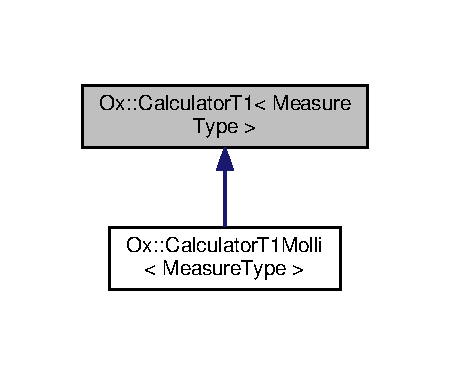
\includegraphics[width=216pt]{class_ox_1_1_calculator_t1__inherit__graph}
\end{center}
\end{figure}
\subsection*{Public Member Functions}
\begin{DoxyCompactItemize}
\item 
virtual int \hyperlink{class_ox_1_1_calculator_t1_af8b7d97caa1f197c937942c8ebc5ae7b}{prepare\-To\-Calculate} ()
\item 
virtual int \hyperlink{class_ox_1_1_calculator_t1_ab8d5ec3f03e070ca11d3accb59a92299}{calculate} ()=0
\item 
\hyperlink{class_ox_1_1_functions_t1}{Functions\-T1}$<$ Measure\-Type $>$ $\ast$ \hyperlink{class_ox_1_1_calculator_t1_a34cee88c8f78b6486ebbfc910559717b}{get\-Functions\-T1} () const 
\item 
\hyperlink{class_ox_1_1_fitter}{Fitter}$<$ Measure\-Type $>$ $\ast$ \hyperlink{class_ox_1_1_calculator_t1_a57f0218fb065b685f4ed5f80051517bd}{get\-Fitter} () const 
\item 
\hyperlink{class_ox_1_1_start_point_calculator}{Start\-Point\-Calculator}\\*
$<$ Measure\-Type $>$ $\ast$ \hyperlink{class_ox_1_1_calculator_t1_a2ee52aac70f34defc99373d5f9f1ed8a}{get\-Start\-Point\-Calculator} () const 
\item 
\hyperlink{class_ox_1_1_sign_calculator}{Sign\-Calculator}$<$ Measure\-Type $>$ $\ast$ \hyperlink{class_ox_1_1_calculator_t1_affc80bde70a6f44f2474e9e0606ba3e0}{get\-Sign\-Calculator} () const 
\item 
const Measure\-Type $\ast$ \hyperlink{class_ox_1_1_calculator_t1_a7179ab384f0ff7f9bf28dc492672da00}{get\-Inv\-Times} () const 
\item 
\hypertarget{class_ox_1_1_calculator_t1_ae892db0c62023dcafbfe6cc2d7877919}{const Measure\-Type $\ast$ {\bfseries get\-Echo\-Times} () const }\label{class_ox_1_1_calculator_t1_ae892db0c62023dcafbfe6cc2d7877919}

\item 
\hypertarget{class_ox_1_1_calculator_t1_aaa68c32a3bba3f994cf00f5c41551952}{const Measure\-Type $\ast$ {\bfseries get\-Rep\-Times} () const }\label{class_ox_1_1_calculator_t1_aaa68c32a3bba3f994cf00f5c41551952}

\item 
\hypertarget{class_ox_1_1_calculator_t1_ac75dbb9b03f6350c19c1551c2bd4bf47}{const Measure\-Type $\ast$ {\bfseries get\-Rel\-Acq\-Times} () const }\label{class_ox_1_1_calculator_t1_ac75dbb9b03f6350c19c1551c2bd4bf47}

\item 
const Measure\-Type $\ast$ \hyperlink{class_ox_1_1_calculator_t1_a7a8fbda407b35212f781640e7cee9f2c}{get\-Sig\-Mag} () const 
\item 
const Measure\-Type $\ast$ \hyperlink{class_ox_1_1_calculator_t1_a1208138a5257482a5f3acc308f3bfd5a}{get\-Sig\-Pha} () const 
\item 
\hypertarget{class_ox_1_1_calculator_t1_a7048aabe616f4ab4b0746d07b38acfa5}{Measure\-Type $\ast$ {\bfseries get\-Signal} () const }\label{class_ox_1_1_calculator_t1_a7048aabe616f4ab4b0746d07b38acfa5}

\item 
\hypertarget{class_ox_1_1_calculator_t1_a1fb7d7a8ab324b807447a5757d8e20f9}{Measure\-Type $\ast$ {\bfseries get\-Signs} () const }\label{class_ox_1_1_calculator_t1_a1fb7d7a8ab324b807447a5757d8e20f9}

\item 
\hypertarget{class_ox_1_1_calculator_t1_a4d430a63b313f8ae1197a27842e87d47}{Measure\-Type $\ast$ {\bfseries get\-Start\-Point} ()}\label{class_ox_1_1_calculator_t1_a4d430a63b313f8ae1197a27842e87d47}

\item 
\hypertarget{class_ox_1_1_calculator_t1_a55406cd104fb7d67925ece789161e2c9}{const \hyperlink{struct_ox_1_1_calculator_t1_results}{Calculator\-T1\-Results}\\*
$<$ Measure\-Type $>$ {\bfseries get\-Results} () const }\label{class_ox_1_1_calculator_t1_a55406cd104fb7d67925ece789161e2c9}

\item 
\hypertarget{class_ox_1_1_calculator_t1_a3b66db06485b8031bcface5524d8c081}{Measure\-Type {\bfseries get\-Mean\-Cut\-Off} () const }\label{class_ox_1_1_calculator_t1_a3b66db06485b8031bcface5524d8c081}

\item 
int \hyperlink{class_ox_1_1_calculator_t1_a8a11b3b6c0dcbc461c11dc55600d7992}{get\-N\-Samples} () const 
\item 
int \hyperlink{class_ox_1_1_calculator_t1_a7523942a79b9ee44b2b5d81d5836b54d}{get\-N\-Dims} () const 
\item 
\hypertarget{class_ox_1_1_calculator_t1_a88e23f6ffa2903dc14a6133a90203f02}{void {\bfseries set\-Functions\-T1} (\hyperlink{class_ox_1_1_functions_t1}{Functions\-T1}$<$ Measure\-Type $>$ $\ast$\-\_\-\-Functions\-T1)}\label{class_ox_1_1_calculator_t1_a88e23f6ffa2903dc14a6133a90203f02}

\item 
\hypertarget{class_ox_1_1_calculator_t1_a106746ffcc08288c933c4dc210589f35}{void {\bfseries set\-Fitter} (\hyperlink{class_ox_1_1_fitter}{Fitter}$<$ Measure\-Type $>$ $\ast$\-\_\-\-Fitter)}\label{class_ox_1_1_calculator_t1_a106746ffcc08288c933c4dc210589f35}

\item 
\hypertarget{class_ox_1_1_calculator_t1_ae043a486f1db48e46a3e011e4a3d76b3}{void {\bfseries set\-Sign\-Calculator} (\hyperlink{class_ox_1_1_sign_calculator}{Sign\-Calculator}$<$ Measure\-Type $>$ $\ast$\-\_\-\-Sign\-Calculator)}\label{class_ox_1_1_calculator_t1_ae043a486f1db48e46a3e011e4a3d76b3}

\item 
\hypertarget{class_ox_1_1_calculator_t1_a89628a47da5bf7baddcd87f687613096}{void {\bfseries set\-Start\-Point\-Calculator} (\hyperlink{class_ox_1_1_start_point_calculator}{Start\-Point\-Calculator}$<$ Measure\-Type $>$ $\ast$\-\_\-\-Start\-Point\-Calculator)}\label{class_ox_1_1_calculator_t1_a89628a47da5bf7baddcd87f687613096}

\item 
\hypertarget{class_ox_1_1_calculator_t1_a102f4865fc2424e6f30bcbd5bf3580f3}{virtual void {\bfseries set\-Inv\-Times} (const Measure\-Type $\ast$\-\_\-\-Inv\-Times)}\label{class_ox_1_1_calculator_t1_a102f4865fc2424e6f30bcbd5bf3580f3}

\item 
\hypertarget{class_ox_1_1_calculator_t1_a4d0327b2105ef6b99cfacb5d37075a5a}{virtual void {\bfseries set\-Sig\-Mag} (const Measure\-Type $\ast$\-\_\-\-Sig\-Mag)}\label{class_ox_1_1_calculator_t1_a4d0327b2105ef6b99cfacb5d37075a5a}

\item 
\hypertarget{class_ox_1_1_calculator_t1_a81b313cfacfd8880e39c0e2cd87c912c}{virtual void {\bfseries set\-Sig\-Pha} (const Measure\-Type $\ast$\-\_\-\-Sig\-Pha)}\label{class_ox_1_1_calculator_t1_a81b313cfacfd8880e39c0e2cd87c912c}

\item 
\hypertarget{class_ox_1_1_calculator_t1_a08da2ecf1ea83b83854fbe09a03de839}{virtual void {\bfseries set\-Mean\-Cut\-Off} (Measure\-Type \-\_\-\-Mean\-Cut\-Off)}\label{class_ox_1_1_calculator_t1_a08da2ecf1ea83b83854fbe09a03de839}

\item 
virtual void \hyperlink{class_ox_1_1_calculator_t1_af5d84e582c3793ebe168f24245f04de1}{set\-N\-Samples} (int \-\_\-n\-Samples)
\item 
virtual void \hyperlink{class_ox_1_1_calculator_t1_abe8decf5aba8ba0de2b6ca76ec9c1386}{set\-N\-Dims} (int \-\_\-n\-Dims)
\item 
\hypertarget{class_ox_1_1_calculator_t1_ab820a5163966ce07d7be7f323ead23ae}{void \hyperlink{class_ox_1_1_calculator_t1_ab820a5163966ce07d7be7f323ead23ae}{disp} ()}\label{class_ox_1_1_calculator_t1_ab820a5163966ce07d7be7f323ead23ae}

\begin{DoxyCompactList}\small\item\em show me your \hyperlink{class_ox_1_1_functions_t1}{Functions\-T1} \end{DoxyCompactList}\item 
\hypertarget{class_ox_1_1_calculator_t1_a11f02c5b0ae3f9b0f8a74044a170ee18}{void \hyperlink{class_ox_1_1_calculator_t1_a11f02c5b0ae3f9b0f8a74044a170ee18}{set\-All\-Pointers\-To\-Null} ()}\label{class_ox_1_1_calculator_t1_a11f02c5b0ae3f9b0f8a74044a170ee18}

\begin{DoxyCompactList}\small\item\em set all the pointers to zero \end{DoxyCompactList}\item 
\hypertarget{class_ox_1_1_calculator_t1_aee286228db734cdd8c6c0686b85fa938}{\hyperlink{class_ox_1_1_calculator_t1_aee286228db734cdd8c6c0686b85fa938}{Calculator\-T1} ()}\label{class_ox_1_1_calculator_t1_aee286228db734cdd8c6c0686b85fa938}

\begin{DoxyCompactList}\small\item\em constructor \end{DoxyCompactList}\item 
\hypertarget{class_ox_1_1_calculator_t1_a125d297d484d10d33b8cbe796b7a60c8}{\hyperlink{class_ox_1_1_calculator_t1_a125d297d484d10d33b8cbe796b7a60c8}{Calculator\-T1} (const \hyperlink{class_ox_1_1_calculator_t1}{Calculator\-T1} \&old)}\label{class_ox_1_1_calculator_t1_a125d297d484d10d33b8cbe796b7a60c8}

\begin{DoxyCompactList}\small\item\em copy constructor \end{DoxyCompactList}\item 
virtual \hyperlink{class_ox_1_1_calculator_t1}{Calculator\-T1}\\*
$<$ Measure\-Type $>$ $\ast$ \hyperlink{class_ox_1_1_calculator_t1_a0db8102b4dad27368667e6ec89c6e4f3}{new\-By\-Cloning} ()=0
\item 
\hypertarget{class_ox_1_1_calculator_t1_af5d360f92d3c1b1c2f4241e528451f2e}{virtual \hyperlink{class_ox_1_1_calculator_t1_af5d360f92d3c1b1c2f4241e528451f2e}{$\sim$\-Calculator\-T1} ()}\label{class_ox_1_1_calculator_t1_af5d360f92d3c1b1c2f4241e528451f2e}

\begin{DoxyCompactList}\small\item\em do not forget about the virtual destructor, see \href{https://stackoverflow.com/questions/461203/when-to-use-virtual-destructors}{\tt https\-://stackoverflow.\-com/questions/461203/when-\/to-\/use-\/virtual-\/destructors} \end{DoxyCompactList}\end{DoxyCompactItemize}
\subsection*{Protected Attributes}
\begin{DoxyCompactItemize}
\item 
\hypertarget{class_ox_1_1_calculator_t1_afa4db4321ca3013a14bcbafbf2d6413a}{\hyperlink{struct_ox_1_1_calculator_t1_results}{Calculator\-T1\-Results}$<$ Measure\-Type $>$ {\bfseries \-\_\-\-Results}}\label{class_ox_1_1_calculator_t1_afa4db4321ca3013a14bcbafbf2d6413a}

\item 
\hypertarget{class_ox_1_1_calculator_t1_a3ad93308f17209680d93b727a90a23ee}{\hyperlink{class_ox_1_1_functions_t1}{Functions\-T1}$<$ Measure\-Type $>$ $\ast$ {\bfseries \-\_\-\-Functions\-T1}}\label{class_ox_1_1_calculator_t1_a3ad93308f17209680d93b727a90a23ee}

\item 
\hypertarget{class_ox_1_1_calculator_t1_a4863afe5f79555d5c6c31f6726d18578}{\hyperlink{class_ox_1_1_fitter}{Fitter}$<$ Measure\-Type $>$ $\ast$ {\bfseries \-\_\-\-Fitter}}\label{class_ox_1_1_calculator_t1_a4863afe5f79555d5c6c31f6726d18578}

\item 
\hypertarget{class_ox_1_1_calculator_t1_a6408fb35f4aeb4793bef57b491f8fa89}{\hyperlink{class_ox_1_1_sign_calculator}{Sign\-Calculator}$<$ Measure\-Type $>$ $\ast$ {\bfseries \-\_\-\-Sign\-Calculator}}\label{class_ox_1_1_calculator_t1_a6408fb35f4aeb4793bef57b491f8fa89}

\item 
\hypertarget{class_ox_1_1_calculator_t1_a6487bcc203c83566702a12a382ebe97f}{\hyperlink{class_ox_1_1_start_point_calculator}{Start\-Point\-Calculator}\\*
$<$ Measure\-Type $>$ $\ast$ {\bfseries \-\_\-\-Start\-Point\-Calculator}}\label{class_ox_1_1_calculator_t1_a6487bcc203c83566702a12a382ebe97f}

\item 
\hypertarget{class_ox_1_1_calculator_t1_ad97a2f1d28c9ffb68b9aa1f50bf85553}{const Measure\-Type $\ast$ {\bfseries \-\_\-\-Inv\-Times}}\label{class_ox_1_1_calculator_t1_ad97a2f1d28c9ffb68b9aa1f50bf85553}

\item 
\hypertarget{class_ox_1_1_calculator_t1_ab8d0c95f394ec1c5c0d765ae2c89df71}{const Measure\-Type $\ast$ {\bfseries \-\_\-\-Echo\-Times}}\label{class_ox_1_1_calculator_t1_ab8d0c95f394ec1c5c0d765ae2c89df71}

\item 
\hypertarget{class_ox_1_1_calculator_t1_a3ca64a023adf3ab3770907057e5ae430}{const Measure\-Type $\ast$ {\bfseries \-\_\-\-Rep\-Times}}\label{class_ox_1_1_calculator_t1_a3ca64a023adf3ab3770907057e5ae430}

\item 
\hypertarget{class_ox_1_1_calculator_t1_ad4831b39c7c92ec666ed9c493edf86db}{const Measure\-Type $\ast$ {\bfseries \-\_\-\-Rel\-Acq\-Times}}\label{class_ox_1_1_calculator_t1_ad4831b39c7c92ec666ed9c493edf86db}

\item 
\hypertarget{class_ox_1_1_calculator_t1_ac900082bed7219ecabb490b2c9049c4b}{const Measure\-Type $\ast$ {\bfseries \-\_\-\-Sig\-Mag}}\label{class_ox_1_1_calculator_t1_ac900082bed7219ecabb490b2c9049c4b}

\item 
\hypertarget{class_ox_1_1_calculator_t1_accb0c7f216c13789a8406d8f588f3280}{const Measure\-Type $\ast$ {\bfseries \-\_\-\-Sig\-Pha}}\label{class_ox_1_1_calculator_t1_accb0c7f216c13789a8406d8f588f3280}

\item 
\hypertarget{class_ox_1_1_calculator_t1_ae3a82567e3036dfa970c35e542ea0efc}{Measure\-Type $\ast$ {\bfseries \-\_\-\-Signal}}\label{class_ox_1_1_calculator_t1_ae3a82567e3036dfa970c35e542ea0efc}

\item 
\hypertarget{class_ox_1_1_calculator_t1_ae770bf1df65f217e264bc680e4376d09}{Measure\-Type $\ast$ {\bfseries \-\_\-\-Signs}}\label{class_ox_1_1_calculator_t1_ae770bf1df65f217e264bc680e4376d09}

\item 
\hypertarget{class_ox_1_1_calculator_t1_add1647551932c3bce7dc8a58fa445251}{Measure\-Type $\ast$ {\bfseries \-\_\-\-Start\-Point}}\label{class_ox_1_1_calculator_t1_add1647551932c3bce7dc8a58fa445251}

\item 
\hypertarget{class_ox_1_1_calculator_t1_a77afa72c6add367c72871e4662bf1325}{int {\bfseries \-\_\-n\-Samples}}\label{class_ox_1_1_calculator_t1_a77afa72c6add367c72871e4662bf1325}

\item 
\hypertarget{class_ox_1_1_calculator_t1_a8ca448ebef97ec9e98b7fd955dfcc132}{int {\bfseries \-\_\-n\-Dims}}\label{class_ox_1_1_calculator_t1_a8ca448ebef97ec9e98b7fd955dfcc132}

\item 
\hypertarget{class_ox_1_1_calculator_t1_a091c2674b79e1c0374637eff90e2becb}{Measure\-Type {\bfseries \-\_\-\-Mean\-Cut\-Off}}\label{class_ox_1_1_calculator_t1_a091c2674b79e1c0374637eff90e2becb}

\end{DoxyCompactItemize}
\subsection*{Static Protected Attributes}
\begin{DoxyCompactItemize}
\item 
\hypertarget{class_ox_1_1_calculator_t1_ab72a428970df42c8a0c1cc4120a45338}{static const int {\bfseries M\-A\-X\-\_\-\-T1\-\_\-\-T\-R\-E\-S\-H\-O\-L\-D} = 4000}\label{class_ox_1_1_calculator_t1_ab72a428970df42c8a0c1cc4120a45338}

\end{DoxyCompactItemize}


\subsection{Detailed Description}
\subsubsection*{template$<$typename Measure\-Type$>$class Ox\-::\-Calculator\-T1$<$ Measure\-Type $>$}


\begin{DoxyTemplParams}{Template Parameters}
{\em Measure\-Type} & \\
\hline
\end{DoxyTemplParams}


\subsection{Member Function Documentation}
\hypertarget{class_ox_1_1_calculator_t1_ab8d5ec3f03e070ca11d3accb59a92299}{\index{Ox\-::\-Calculator\-T1@{Ox\-::\-Calculator\-T1}!calculate@{calculate}}
\index{calculate@{calculate}!Ox::CalculatorT1@{Ox\-::\-Calculator\-T1}}
\subsubsection[{calculate}]{\setlength{\rightskip}{0pt plus 5cm}template$<$typename Measure\-Type$>$ virtual int {\bf Ox\-::\-Calculator\-T1}$<$ Measure\-Type $>$\-::calculate (
\begin{DoxyParamCaption}
{}
\end{DoxyParamCaption}
)\hspace{0.3cm}{\ttfamily [pure virtual]}}}\label{class_ox_1_1_calculator_t1_ab8d5ec3f03e070ca11d3accb59a92299}
the most important function of this class \begin{DoxyReturn}{Returns}
success/failure 
\end{DoxyReturn}


Implemented in \hyperlink{class_ox_1_1_calculator_t1_shmolli_ac689ebbf27f95f6fa2559cc13a824db0}{Ox\-::\-Calculator\-T1\-Shmolli$<$ Measure\-Type $>$}, and \hyperlink{class_ox_1_1_calculator_t1_molli_a6f15bc9c026305248c927d62748903bf}{Ox\-::\-Calculator\-T1\-Molli$<$ Measure\-Type $>$}.

\hypertarget{class_ox_1_1_calculator_t1_a57f0218fb065b685f4ed5f80051517bd}{\index{Ox\-::\-Calculator\-T1@{Ox\-::\-Calculator\-T1}!get\-Fitter@{get\-Fitter}}
\index{get\-Fitter@{get\-Fitter}!Ox::CalculatorT1@{Ox\-::\-Calculator\-T1}}
\subsubsection[{get\-Fitter}]{\setlength{\rightskip}{0pt plus 5cm}template$<$typename Measure\-Type $>$ {\bf Fitter}$<$ Measure\-Type $>$ $\ast$ {\bf Ox\-::\-Calculator\-T1}$<$ Measure\-Type $>$\-::get\-Fitter (
\begin{DoxyParamCaption}
{}
\end{DoxyParamCaption}
) const}}\label{class_ox_1_1_calculator_t1_a57f0218fb065b685f4ed5f80051517bd}
/throw exception if \-\_\-\-Fitter == 0 \begin{DoxyReturn}{Returns}

\end{DoxyReturn}
\hypertarget{class_ox_1_1_calculator_t1_a34cee88c8f78b6486ebbfc910559717b}{\index{Ox\-::\-Calculator\-T1@{Ox\-::\-Calculator\-T1}!get\-Functions\-T1@{get\-Functions\-T1}}
\index{get\-Functions\-T1@{get\-Functions\-T1}!Ox::CalculatorT1@{Ox\-::\-Calculator\-T1}}
\subsubsection[{get\-Functions\-T1}]{\setlength{\rightskip}{0pt plus 5cm}template$<$typename Measure\-Type $>$ {\bf Functions\-T1}$<$ Measure\-Type $>$ $\ast$ {\bf Ox\-::\-Calculator\-T1}$<$ Measure\-Type $>$\-::get\-Functions\-T1 (
\begin{DoxyParamCaption}
{}
\end{DoxyParamCaption}
) const}}\label{class_ox_1_1_calculator_t1_a34cee88c8f78b6486ebbfc910559717b}
/throw exception if \-\_\-\-Functions\-T1 == 0 \begin{DoxyReturn}{Returns}

\end{DoxyReturn}
\hypertarget{class_ox_1_1_calculator_t1_a7179ab384f0ff7f9bf28dc492672da00}{\index{Ox\-::\-Calculator\-T1@{Ox\-::\-Calculator\-T1}!get\-Inv\-Times@{get\-Inv\-Times}}
\index{get\-Inv\-Times@{get\-Inv\-Times}!Ox::CalculatorT1@{Ox\-::\-Calculator\-T1}}
\subsubsection[{get\-Inv\-Times}]{\setlength{\rightskip}{0pt plus 5cm}template$<$typename Measure\-Type $>$ const Measure\-Type $\ast$ {\bf Ox\-::\-Calculator\-T1}$<$ Measure\-Type $>$\-::get\-Inv\-Times (
\begin{DoxyParamCaption}
{}
\end{DoxyParamCaption}
) const}}\label{class_ox_1_1_calculator_t1_a7179ab384f0ff7f9bf28dc492672da00}
/throw exception if \-\_\-\-Inv\-Times == 0 \begin{DoxyReturn}{Returns}

\end{DoxyReturn}
\hypertarget{class_ox_1_1_calculator_t1_a7523942a79b9ee44b2b5d81d5836b54d}{\index{Ox\-::\-Calculator\-T1@{Ox\-::\-Calculator\-T1}!get\-N\-Dims@{get\-N\-Dims}}
\index{get\-N\-Dims@{get\-N\-Dims}!Ox::CalculatorT1@{Ox\-::\-Calculator\-T1}}
\subsubsection[{get\-N\-Dims}]{\setlength{\rightskip}{0pt plus 5cm}template$<$typename Measure\-Type $>$ int {\bf Ox\-::\-Calculator\-T1}$<$ Measure\-Type $>$\-::get\-N\-Dims (
\begin{DoxyParamCaption}
{}
\end{DoxyParamCaption}
) const}}\label{class_ox_1_1_calculator_t1_a7523942a79b9ee44b2b5d81d5836b54d}
/throw exception if \-\_\-n\-Dims == 0 \begin{DoxyReturn}{Returns}

\end{DoxyReturn}
\hypertarget{class_ox_1_1_calculator_t1_a8a11b3b6c0dcbc461c11dc55600d7992}{\index{Ox\-::\-Calculator\-T1@{Ox\-::\-Calculator\-T1}!get\-N\-Samples@{get\-N\-Samples}}
\index{get\-N\-Samples@{get\-N\-Samples}!Ox::CalculatorT1@{Ox\-::\-Calculator\-T1}}
\subsubsection[{get\-N\-Samples}]{\setlength{\rightskip}{0pt plus 5cm}template$<$typename Measure\-Type $>$ int {\bf Ox\-::\-Calculator\-T1}$<$ Measure\-Type $>$\-::get\-N\-Samples (
\begin{DoxyParamCaption}
{}
\end{DoxyParamCaption}
) const}}\label{class_ox_1_1_calculator_t1_a8a11b3b6c0dcbc461c11dc55600d7992}
/throw exception if \-\_\-n\-Samples == 0 \begin{DoxyReturn}{Returns}

\end{DoxyReturn}
\hypertarget{class_ox_1_1_calculator_t1_a7a8fbda407b35212f781640e7cee9f2c}{\index{Ox\-::\-Calculator\-T1@{Ox\-::\-Calculator\-T1}!get\-Sig\-Mag@{get\-Sig\-Mag}}
\index{get\-Sig\-Mag@{get\-Sig\-Mag}!Ox::CalculatorT1@{Ox\-::\-Calculator\-T1}}
\subsubsection[{get\-Sig\-Mag}]{\setlength{\rightskip}{0pt plus 5cm}template$<$typename Measure\-Type $>$ const Measure\-Type $\ast$ {\bf Ox\-::\-Calculator\-T1}$<$ Measure\-Type $>$\-::get\-Sig\-Mag (
\begin{DoxyParamCaption}
{}
\end{DoxyParamCaption}
) const}}\label{class_ox_1_1_calculator_t1_a7a8fbda407b35212f781640e7cee9f2c}
/throw exception if \-\_\-\-Sig\-Mag == 0 \begin{DoxyReturn}{Returns}

\end{DoxyReturn}
\hypertarget{class_ox_1_1_calculator_t1_affc80bde70a6f44f2474e9e0606ba3e0}{\index{Ox\-::\-Calculator\-T1@{Ox\-::\-Calculator\-T1}!get\-Sign\-Calculator@{get\-Sign\-Calculator}}
\index{get\-Sign\-Calculator@{get\-Sign\-Calculator}!Ox::CalculatorT1@{Ox\-::\-Calculator\-T1}}
\subsubsection[{get\-Sign\-Calculator}]{\setlength{\rightskip}{0pt plus 5cm}template$<$typename Measure\-Type $>$ {\bf Sign\-Calculator}$<$ Measure\-Type $>$ $\ast$ {\bf Ox\-::\-Calculator\-T1}$<$ Measure\-Type $>$\-::get\-Sign\-Calculator (
\begin{DoxyParamCaption}
{}
\end{DoxyParamCaption}
) const}}\label{class_ox_1_1_calculator_t1_affc80bde70a6f44f2474e9e0606ba3e0}
/throw exception if \-\_\-\-Sign\-Calculator == 0 \begin{DoxyReturn}{Returns}

\end{DoxyReturn}
\hypertarget{class_ox_1_1_calculator_t1_a1208138a5257482a5f3acc308f3bfd5a}{\index{Ox\-::\-Calculator\-T1@{Ox\-::\-Calculator\-T1}!get\-Sig\-Pha@{get\-Sig\-Pha}}
\index{get\-Sig\-Pha@{get\-Sig\-Pha}!Ox::CalculatorT1@{Ox\-::\-Calculator\-T1}}
\subsubsection[{get\-Sig\-Pha}]{\setlength{\rightskip}{0pt plus 5cm}template$<$typename Measure\-Type $>$ const Measure\-Type $\ast$ {\bf Ox\-::\-Calculator\-T1}$<$ Measure\-Type $>$\-::get\-Sig\-Pha (
\begin{DoxyParamCaption}
{}
\end{DoxyParamCaption}
) const}}\label{class_ox_1_1_calculator_t1_a1208138a5257482a5f3acc308f3bfd5a}
does not have to be set \begin{DoxyReturn}{Returns}
Sig\-Pha pointer, can be 0 (N\-U\-L\-L) 
\end{DoxyReturn}
\hypertarget{class_ox_1_1_calculator_t1_a2ee52aac70f34defc99373d5f9f1ed8a}{\index{Ox\-::\-Calculator\-T1@{Ox\-::\-Calculator\-T1}!get\-Start\-Point\-Calculator@{get\-Start\-Point\-Calculator}}
\index{get\-Start\-Point\-Calculator@{get\-Start\-Point\-Calculator}!Ox::CalculatorT1@{Ox\-::\-Calculator\-T1}}
\subsubsection[{get\-Start\-Point\-Calculator}]{\setlength{\rightskip}{0pt plus 5cm}template$<$typename Measure\-Type $>$ {\bf Start\-Point\-Calculator}$<$ Measure\-Type $>$ $\ast$ {\bf Ox\-::\-Calculator\-T1}$<$ Measure\-Type $>$\-::get\-Start\-Point\-Calculator (
\begin{DoxyParamCaption}
{}
\end{DoxyParamCaption}
) const}}\label{class_ox_1_1_calculator_t1_a2ee52aac70f34defc99373d5f9f1ed8a}
/throw exception if \-\_\-\-Start\-Point\-Calculator == 0 \begin{DoxyReturn}{Returns}

\end{DoxyReturn}
\hypertarget{class_ox_1_1_calculator_t1_a0db8102b4dad27368667e6ec89c6e4f3}{\index{Ox\-::\-Calculator\-T1@{Ox\-::\-Calculator\-T1}!new\-By\-Cloning@{new\-By\-Cloning}}
\index{new\-By\-Cloning@{new\-By\-Cloning}!Ox::CalculatorT1@{Ox\-::\-Calculator\-T1}}
\subsubsection[{new\-By\-Cloning}]{\setlength{\rightskip}{0pt plus 5cm}template$<$typename Measure\-Type$>$ virtual {\bf Calculator\-T1}$<$Measure\-Type$>$$\ast$ {\bf Ox\-::\-Calculator\-T1}$<$ Measure\-Type $>$\-::new\-By\-Cloning (
\begin{DoxyParamCaption}
{}
\end{DoxyParamCaption}
)\hspace{0.3cm}{\ttfamily [pure virtual]}}}\label{class_ox_1_1_calculator_t1_a0db8102b4dad27368667e6ec89c6e4f3}
cloning \begin{DoxyReturn}{Returns}

\end{DoxyReturn}


Implemented in \hyperlink{class_ox_1_1_calculator_t1_molli_ae0fde362fbe16c4c40dee96330b4a676}{Ox\-::\-Calculator\-T1\-Molli$<$ Measure\-Type $>$}, and \hyperlink{class_ox_1_1_calculator_t1_shmolli_a5fa5fd5685a5566e605a1ee93569ac29}{Ox\-::\-Calculator\-T1\-Shmolli$<$ Measure\-Type $>$}.

\hypertarget{class_ox_1_1_calculator_t1_af8b7d97caa1f197c937942c8ebc5ae7b}{\index{Ox\-::\-Calculator\-T1@{Ox\-::\-Calculator\-T1}!prepare\-To\-Calculate@{prepare\-To\-Calculate}}
\index{prepare\-To\-Calculate@{prepare\-To\-Calculate}!Ox::CalculatorT1@{Ox\-::\-Calculator\-T1}}
\subsubsection[{prepare\-To\-Calculate}]{\setlength{\rightskip}{0pt plus 5cm}template$<$typename Measure\-Type $>$ int {\bf Ox\-::\-Calculator\-T1}$<$ Measure\-Type $>$\-::prepare\-To\-Calculate (
\begin{DoxyParamCaption}
{}
\end{DoxyParamCaption}
)\hspace{0.3cm}{\ttfamily [virtual]}}}\label{class_ox_1_1_calculator_t1_af8b7d97caa1f197c937942c8ebc5ae7b}
do all the checks and prepare to do the calculation, for example calc signal/signs and \-\_\-\-T\-R\-Raverage\-H\-B \begin{DoxyReturn}{Returns}
success/failure 
\end{DoxyReturn}


Reimplemented in \hyperlink{class_ox_1_1_calculator_t1_shmolli_a6464c63f20ecd9de842d722e5d9d2866}{Ox\-::\-Calculator\-T1\-Shmolli$<$ Measure\-Type $>$}.

\hypertarget{class_ox_1_1_calculator_t1_abe8decf5aba8ba0de2b6ca76ec9c1386}{\index{Ox\-::\-Calculator\-T1@{Ox\-::\-Calculator\-T1}!set\-N\-Dims@{set\-N\-Dims}}
\index{set\-N\-Dims@{set\-N\-Dims}!Ox::CalculatorT1@{Ox\-::\-Calculator\-T1}}
\subsubsection[{set\-N\-Dims}]{\setlength{\rightskip}{0pt plus 5cm}template$<$typename Measure\-Type $>$ void {\bf Ox\-::\-Calculator\-T1}$<$ Measure\-Type $>$\-::set\-N\-Dims (
\begin{DoxyParamCaption}
\item[{int}]{\-\_\-n\-Dims}
\end{DoxyParamCaption}
)\hspace{0.3cm}{\ttfamily [virtual]}}}\label{class_ox_1_1_calculator_t1_abe8decf5aba8ba0de2b6ca76ec9c1386}
\-\_\-\-Start\-Point is allocated here!!! 
\begin{DoxyParams}{Parameters}
{\em \-\_\-n\-Dims} & \\
\hline
\end{DoxyParams}
\hypertarget{class_ox_1_1_calculator_t1_af5d84e582c3793ebe168f24245f04de1}{\index{Ox\-::\-Calculator\-T1@{Ox\-::\-Calculator\-T1}!set\-N\-Samples@{set\-N\-Samples}}
\index{set\-N\-Samples@{set\-N\-Samples}!Ox::CalculatorT1@{Ox\-::\-Calculator\-T1}}
\subsubsection[{set\-N\-Samples}]{\setlength{\rightskip}{0pt plus 5cm}template$<$typename Measure\-Type $>$ void {\bf Ox\-::\-Calculator\-T1}$<$ Measure\-Type $>$\-::set\-N\-Samples (
\begin{DoxyParamCaption}
\item[{int}]{\-\_\-n\-Samples}
\end{DoxyParamCaption}
)\hspace{0.3cm}{\ttfamily [virtual]}}}\label{class_ox_1_1_calculator_t1_af5d84e582c3793ebe168f24245f04de1}
\-\_\-\-Signal and \-\_\-\-Signs are allocated here!!! 
\begin{DoxyParams}{Parameters}
{\em \-\_\-n\-Samples} & \\
\hline
\end{DoxyParams}


The documentation for this class was generated from the following files\-:\begin{DoxyCompactItemize}
\item 
lib/Ox\-Calculator\-T1.\-h\item 
lib/Ox\-Calculator\-T1.\-hxx\end{DoxyCompactItemize}

\hypertarget{class_ox_1_1_calculator_t1_molli}{\section{Ox\-:\-:Calculator\-T1\-Molli$<$ Measure\-Type $>$ Class Template Reference}
\label{class_ox_1_1_calculator_t1_molli}\index{Ox\-::\-Calculator\-T1\-Molli$<$ Measure\-Type $>$@{Ox\-::\-Calculator\-T1\-Molli$<$ Measure\-Type $>$}}
}


{\ttfamily \#include $<$Ox\-Calculator\-T1\-Molli.\-h$>$}



Inheritance diagram for Ox\-:\-:Calculator\-T1\-Molli$<$ Measure\-Type $>$\-:
\nopagebreak
\begin{figure}[H]
\begin{center}
\leavevmode
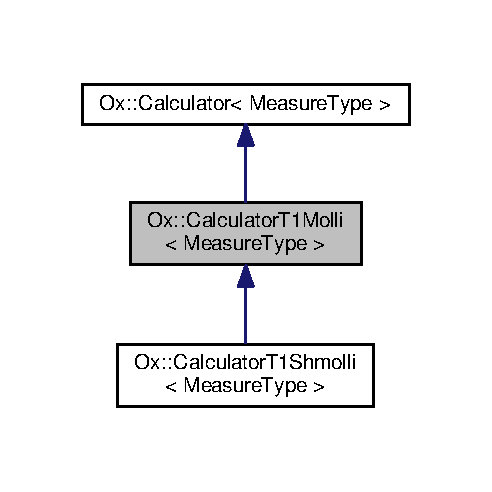
\includegraphics[width=216pt]{class_ox_1_1_calculator_t1_molli__inherit__graph}
\end{center}
\end{figure}


Collaboration diagram for Ox\-:\-:Calculator\-T1\-Molli$<$ Measure\-Type $>$\-:
\nopagebreak
\begin{figure}[H]
\begin{center}
\leavevmode
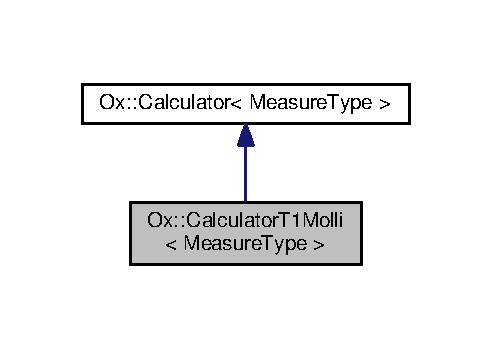
\includegraphics[width=216pt]{class_ox_1_1_calculator_t1_molli__coll__graph}
\end{center}
\end{figure}
\subsection*{Public Member Functions}
\begin{DoxyCompactItemize}
\item 
virtual int \hyperlink{class_ox_1_1_calculator_t1_molli_a6f15bc9c026305248c927d62748903bf}{calculate} ()
\item 
virtual \hyperlink{struct_ox_1_1_calculator_t1_results}{Calculator\-T1\-Results}\\*
$<$ Measure\-Type $>$ \hyperlink{class_ox_1_1_calculator_t1_molli_a9cb84f5e8680e1bf6c3543846fc90c4d}{calculate\-Molli} (int n\-Samples, const Measure\-Type $\ast$inv\-Times, Measure\-Type $\ast$signal, Measure\-Type $\ast$signs)
\item 
Measure\-Type \hyperlink{class_ox_1_1_calculator_t1_molli_a9c9238dd8a96e06d3e0a96810377b90b}{calculate\-R2\-Abs\-From\-Model} (int n\-Samples, const Measure\-Type $\ast$inv\-Times, const Measure\-Type $\ast$signal, const Measure\-Type $\ast$parameters)
\item 
int \hyperlink{class_ox_1_1_calculator_t1_molli_a030582bca754a7b81febfae53fe0c10c}{calculate\-Covariance\-Matrix} (const Measure\-Type $\ast$parameters, Measure\-Type $\ast$covariance\-Matrix)
\item 
int \hyperlink{class_ox_1_1_calculator_t1_molli_aec374fc512aa3b109138f0c16c53a171}{calculate\-Inv\-Covariance\-Matrix} (const Measure\-Type $\ast$inv\-Times, const Measure\-Type $\ast$residuals, const Measure\-Type $\ast$parameters, Measure\-Type $\ast$inv\-Covariance\-Matrix)
\item 
bool \hyperlink{class_ox_1_1_calculator_t1_molli_a06d8579492ee063b129b489e638333be}{get\-Do\-Calculate\-S\-D\-Map} () const 
\item 
void \hyperlink{class_ox_1_1_calculator_t1_molli_a65a51dcadaafdefc576201de535f8810}{set\-Do\-Calculate\-S\-D\-Map} (bool \-\_\-\-Do\-Calculate\-S\-D\-Map)
\item 
\hyperlink{class_ox_1_1_calculator_t1_molli_ab1892de078822ea106fcaebcf81047be}{Calculator\-T1\-Molli} ()
\item 
virtual \hyperlink{class_ox_1_1_calculator_t1}{Calculator\-T1}\\*
$<$ Measure\-Type $>$ $\ast$ \hyperlink{class_ox_1_1_calculator_t1_molli_ae0fde362fbe16c4c40dee96330b4a676}{new\-By\-Cloning} ()
\end{DoxyCompactItemize}
\subsection*{Protected Attributes}
\begin{DoxyCompactItemize}
\item 
\hypertarget{class_ox_1_1_calculator_t1_molli_adb4f50cdf9dabf4890b4d28194d0522b}{double {\bfseries Max\-T\-I\-For\-Sign\-Invert}}\label{class_ox_1_1_calculator_t1_molli_adb4f50cdf9dabf4890b4d28194d0522b}

\item 
\hypertarget{class_ox_1_1_calculator_t1_molli_adbe23b503f5695ff35734d2c20972277}{bool {\bfseries \-\_\-\-Do\-Calculate\-S\-D\-Map}}\label{class_ox_1_1_calculator_t1_molli_adbe23b503f5695ff35734d2c20972277}

\end{DoxyCompactItemize}
\subsection*{Additional Inherited Members}


\subsection{Detailed Description}
\subsubsection*{template$<$typename Measure\-Type$>$class Ox\-::\-Calculator\-T1\-Molli$<$ Measure\-Type $>$}


\begin{DoxyTemplParams}{Template Parameters}
{\em Measure\-Type} & \\
\hline
\end{DoxyTemplParams}


\subsection{Constructor \& Destructor Documentation}
\hypertarget{class_ox_1_1_calculator_t1_molli_ab1892de078822ea106fcaebcf81047be}{\index{Ox\-::\-Calculator\-T1\-Molli@{Ox\-::\-Calculator\-T1\-Molli}!Calculator\-T1\-Molli@{Calculator\-T1\-Molli}}
\index{Calculator\-T1\-Molli@{Calculator\-T1\-Molli}!Ox::CalculatorT1Molli@{Ox\-::\-Calculator\-T1\-Molli}}
\subsubsection[{Calculator\-T1\-Molli}]{\setlength{\rightskip}{0pt plus 5cm}template$<$typename Measure\-Type$>$ {\bf Ox\-::\-Calculator\-T1\-Molli}$<$ Measure\-Type $>$\-::{\bf Calculator\-T1\-Molli} (
\begin{DoxyParamCaption}
{}
\end{DoxyParamCaption}
)\hspace{0.3cm}{\ttfamily [inline]}}}\label{class_ox_1_1_calculator_t1_molli_ab1892de078822ea106fcaebcf81047be}
constructor 

\subsection{Member Function Documentation}
\hypertarget{class_ox_1_1_calculator_t1_molli_a6f15bc9c026305248c927d62748903bf}{\index{Ox\-::\-Calculator\-T1\-Molli@{Ox\-::\-Calculator\-T1\-Molli}!calculate@{calculate}}
\index{calculate@{calculate}!Ox::CalculatorT1Molli@{Ox\-::\-Calculator\-T1\-Molli}}
\subsubsection[{calculate}]{\setlength{\rightskip}{0pt plus 5cm}template$<$typename Measure\-Type $>$ int {\bf Ox\-::\-Calculator\-T1\-Molli}$<$ Measure\-Type $>$\-::calculate (
\begin{DoxyParamCaption}
{}
\end{DoxyParamCaption}
)\hspace{0.3cm}{\ttfamily [virtual]}}}\label{class_ox_1_1_calculator_t1_molli_a6f15bc9c026305248c927d62748903bf}
calling \hyperlink{class_ox_1_1_calculator_t1_molli_a9cb84f5e8680e1bf6c3543846fc90c4d}{calculate\-Molli(int n\-Samples, const Measure\-Type$\ast$ inv\-Times, Measure\-Type$\ast$ signal, Measure\-Type$\ast$ signs)} \begin{DoxyReturn}{Returns}
success/failure 
\end{DoxyReturn}


Implements \hyperlink{class_ox_1_1_calculator_t1_ab8d5ec3f03e070ca11d3accb59a92299}{Ox\-::\-Calculator\-T1$<$ Measure\-Type $>$}.



Reimplemented in \hyperlink{class_ox_1_1_calculator_t1_shmolli_ac689ebbf27f95f6fa2559cc13a824db0}{Ox\-::\-Calculator\-T1\-Shmolli$<$ Measure\-Type $>$}.

\hypertarget{class_ox_1_1_calculator_t1_molli_a030582bca754a7b81febfae53fe0c10c}{\index{Ox\-::\-Calculator\-T1\-Molli@{Ox\-::\-Calculator\-T1\-Molli}!calculate\-Covariance\-Matrix@{calculate\-Covariance\-Matrix}}
\index{calculate\-Covariance\-Matrix@{calculate\-Covariance\-Matrix}!Ox::CalculatorT1Molli@{Ox\-::\-Calculator\-T1\-Molli}}
\subsubsection[{calculate\-Covariance\-Matrix}]{\setlength{\rightskip}{0pt plus 5cm}template$<$typename Measure\-Type $>$ int {\bf Ox\-::\-Calculator\-T1\-Molli}$<$ Measure\-Type $>$\-::calculate\-Covariance\-Matrix (
\begin{DoxyParamCaption}
\item[{const Measure\-Type $\ast$}]{parameters, }
\item[{Measure\-Type $\ast$}]{covariance\-Matrix}
\end{DoxyParamCaption}
)}}\label{class_ox_1_1_calculator_t1_molli_a030582bca754a7b81febfae53fe0c10c}
calculate covariance matrix needed for S\-D estimation 
\begin{DoxyParams}{Parameters}
{\em parameters} & \\
\hline
{\em covariance\-Matrix} & \\
\hline
\end{DoxyParams}
\begin{DoxyReturn}{Returns}

\end{DoxyReturn}
\hypertarget{class_ox_1_1_calculator_t1_molli_aec374fc512aa3b109138f0c16c53a171}{\index{Ox\-::\-Calculator\-T1\-Molli@{Ox\-::\-Calculator\-T1\-Molli}!calculate\-Inv\-Covariance\-Matrix@{calculate\-Inv\-Covariance\-Matrix}}
\index{calculate\-Inv\-Covariance\-Matrix@{calculate\-Inv\-Covariance\-Matrix}!Ox::CalculatorT1Molli@{Ox\-::\-Calculator\-T1\-Molli}}
\subsubsection[{calculate\-Inv\-Covariance\-Matrix}]{\setlength{\rightskip}{0pt plus 5cm}template$<$typename Measure\-Type $>$ int {\bf Ox\-::\-Calculator\-T1\-Molli}$<$ Measure\-Type $>$\-::calculate\-Inv\-Covariance\-Matrix (
\begin{DoxyParamCaption}
\item[{const Measure\-Type $\ast$}]{inv\-Times, }
\item[{const Measure\-Type $\ast$}]{residuals, }
\item[{const Measure\-Type $\ast$}]{parameters, }
\item[{Measure\-Type $\ast$}]{inv\-Covariance\-Matrix}
\end{DoxyParamCaption}
)}}\label{class_ox_1_1_calculator_t1_molli_aec374fc512aa3b109138f0c16c53a171}
calculate inverse covariance matrix needed for S\-D estimation 
\begin{DoxyParams}{Parameters}
{\em inv\-Times} & \\
\hline
{\em residuals} & \\
\hline
{\em parameters} & \\
\hline
{\em inv\-Covariance\-Matrix} & \\
\hline
\end{DoxyParams}
\begin{DoxyReturn}{Returns}

\end{DoxyReturn}
\hypertarget{class_ox_1_1_calculator_t1_molli_a9cb84f5e8680e1bf6c3543846fc90c4d}{\index{Ox\-::\-Calculator\-T1\-Molli@{Ox\-::\-Calculator\-T1\-Molli}!calculate\-Molli@{calculate\-Molli}}
\index{calculate\-Molli@{calculate\-Molli}!Ox::CalculatorT1Molli@{Ox\-::\-Calculator\-T1\-Molli}}
\subsubsection[{calculate\-Molli}]{\setlength{\rightskip}{0pt plus 5cm}template$<$typename Measure\-Type $>$ {\bf Calculator\-T1\-Results}$<$ Measure\-Type $>$ {\bf Ox\-::\-Calculator\-T1\-Molli}$<$ Measure\-Type $>$\-::calculate\-Molli (
\begin{DoxyParamCaption}
\item[{int}]{n\-Samples, }
\item[{const Measure\-Type $\ast$}]{inv\-Times, }
\item[{Measure\-Type $\ast$}]{signal, }
\item[{Measure\-Type $\ast$}]{signs}
\end{DoxyParamCaption}
)\hspace{0.3cm}{\ttfamily [virtual]}}}\label{class_ox_1_1_calculator_t1_molli_a9cb84f5e8680e1bf6c3543846fc90c4d}
The most important function of this class It has all the input parameters so that I can call it from the shmolli class 
\begin{DoxyParams}{Parameters}
{\em n\-Samples} & \\
\hline
{\em inv\-Times} & \\
\hline
{\em signal} & \\
\hline
{\em signs} & \\
\hline
\end{DoxyParams}
\begin{DoxyReturn}{Returns}
success/failure 
\end{DoxyReturn}
\hypertarget{class_ox_1_1_calculator_t1_molli_a9c9238dd8a96e06d3e0a96810377b90b}{\index{Ox\-::\-Calculator\-T1\-Molli@{Ox\-::\-Calculator\-T1\-Molli}!calculate\-R2\-Abs\-From\-Model@{calculate\-R2\-Abs\-From\-Model}}
\index{calculate\-R2\-Abs\-From\-Model@{calculate\-R2\-Abs\-From\-Model}!Ox::CalculatorT1Molli@{Ox\-::\-Calculator\-T1\-Molli}}
\subsubsection[{calculate\-R2\-Abs\-From\-Model}]{\setlength{\rightskip}{0pt plus 5cm}template$<$typename Measure\-Type $>$ Measure\-Type {\bf Ox\-::\-Calculator\-T1\-Molli}$<$ Measure\-Type $>$\-::calculate\-R2\-Abs\-From\-Model (
\begin{DoxyParamCaption}
\item[{int}]{n\-Samples, }
\item[{const Measure\-Type $\ast$}]{inv\-Times, }
\item[{const Measure\-Type $\ast$}]{signal, }
\item[{const Measure\-Type $\ast$}]{parameters}
\end{DoxyParamCaption}
)}}\label{class_ox_1_1_calculator_t1_molli_a9c9238dd8a96e06d3e0a96810377b90b}
Calculate goodness of fit map 
\begin{DoxyParams}{Parameters}
{\em n\-Samples} & \\
\hline
{\em inv\-Times} & \\
\hline
{\em signal} & \\
\hline
{\em parameters} & \\
\hline
\end{DoxyParams}
\begin{DoxyReturn}{Returns}

\end{DoxyReturn}
\hypertarget{class_ox_1_1_calculator_t1_molli_a06d8579492ee063b129b489e638333be}{\index{Ox\-::\-Calculator\-T1\-Molli@{Ox\-::\-Calculator\-T1\-Molli}!get\-Do\-Calculate\-S\-D\-Map@{get\-Do\-Calculate\-S\-D\-Map}}
\index{get\-Do\-Calculate\-S\-D\-Map@{get\-Do\-Calculate\-S\-D\-Map}!Ox::CalculatorT1Molli@{Ox\-::\-Calculator\-T1\-Molli}}
\subsubsection[{get\-Do\-Calculate\-S\-D\-Map}]{\setlength{\rightskip}{0pt plus 5cm}template$<$typename Measure\-Type $>$ bool {\bf Ox\-::\-Calculator\-T1\-Molli}$<$ Measure\-Type $>$\-::get\-Do\-Calculate\-S\-D\-Map (
\begin{DoxyParamCaption}
{}
\end{DoxyParamCaption}
) const}}\label{class_ox_1_1_calculator_t1_molli_a06d8579492ee063b129b489e638333be}
\begin{DoxyReturn}{Returns}

\end{DoxyReturn}
\hypertarget{class_ox_1_1_calculator_t1_molli_ae0fde362fbe16c4c40dee96330b4a676}{\index{Ox\-::\-Calculator\-T1\-Molli@{Ox\-::\-Calculator\-T1\-Molli}!new\-By\-Cloning@{new\-By\-Cloning}}
\index{new\-By\-Cloning@{new\-By\-Cloning}!Ox::CalculatorT1Molli@{Ox\-::\-Calculator\-T1\-Molli}}
\subsubsection[{new\-By\-Cloning}]{\setlength{\rightskip}{0pt plus 5cm}template$<$typename Measure\-Type$>$ virtual {\bf Calculator\-T1}$<$Measure\-Type$>$$\ast$ {\bf Ox\-::\-Calculator\-T1\-Molli}$<$ Measure\-Type $>$\-::new\-By\-Cloning (
\begin{DoxyParamCaption}
{}
\end{DoxyParamCaption}
)\hspace{0.3cm}{\ttfamily [inline]}, {\ttfamily [virtual]}}}\label{class_ox_1_1_calculator_t1_molli_ae0fde362fbe16c4c40dee96330b4a676}
cloning \begin{DoxyReturn}{Returns}

\end{DoxyReturn}


Implements \hyperlink{class_ox_1_1_calculator_t1_a0db8102b4dad27368667e6ec89c6e4f3}{Ox\-::\-Calculator\-T1$<$ Measure\-Type $>$}.



Reimplemented in \hyperlink{class_ox_1_1_calculator_t1_shmolli_a5fa5fd5685a5566e605a1ee93569ac29}{Ox\-::\-Calculator\-T1\-Shmolli$<$ Measure\-Type $>$}.

\hypertarget{class_ox_1_1_calculator_t1_molli_a65a51dcadaafdefc576201de535f8810}{\index{Ox\-::\-Calculator\-T1\-Molli@{Ox\-::\-Calculator\-T1\-Molli}!set\-Do\-Calculate\-S\-D\-Map@{set\-Do\-Calculate\-S\-D\-Map}}
\index{set\-Do\-Calculate\-S\-D\-Map@{set\-Do\-Calculate\-S\-D\-Map}!Ox::CalculatorT1Molli@{Ox\-::\-Calculator\-T1\-Molli}}
\subsubsection[{set\-Do\-Calculate\-S\-D\-Map}]{\setlength{\rightskip}{0pt plus 5cm}template$<$typename Measure\-Type $>$ void {\bf Ox\-::\-Calculator\-T1\-Molli}$<$ Measure\-Type $>$\-::set\-Do\-Calculate\-S\-D\-Map (
\begin{DoxyParamCaption}
\item[{bool}]{\-\_\-\-Do\-Calculate\-S\-D\-Map}
\end{DoxyParamCaption}
)}}\label{class_ox_1_1_calculator_t1_molli_a65a51dcadaafdefc576201de535f8810}

\begin{DoxyParams}{Parameters}
{\em \-\_\-\-Do\-Calculate\-S\-D\-Map} & \\
\hline
\end{DoxyParams}


The documentation for this class was generated from the following files\-:\begin{DoxyCompactItemize}
\item 
lib/\hyperlink{_ox_calculator_t1_molli_8h}{Ox\-Calculator\-T1\-Molli.\-h}\item 
lib/\hyperlink{_ox_calculator_t1_molli_8hxx}{Ox\-Calculator\-T1\-Molli.\-hxx}\end{DoxyCompactItemize}

\hypertarget{struct_ox_1_1_calculator_t1_results}{\section{Ox\-:\-:Calculator\-T1\-Results$<$ Measure\-Type $>$ Struct Template Reference}
\label{struct_ox_1_1_calculator_t1_results}\index{Ox\-::\-Calculator\-T1\-Results$<$ Measure\-Type $>$@{Ox\-::\-Calculator\-T1\-Results$<$ Measure\-Type $>$}}
}
\subsection*{Public Member Functions}
\begin{DoxyCompactItemize}
\item 
\hyperlink{struct_ox_1_1_calculator_t1_results_a2ef9ec72b2f7e61bb442fe8e0f61d508}{Calculator\-T1\-Results} ()
\item 
\hypertarget{struct_ox_1_1_calculator_t1_results_a95930b2a41a0caf402b254deaad2353c}{void {\bfseries disp} ()}\label{struct_ox_1_1_calculator_t1_results_a95930b2a41a0caf402b254deaad2353c}

\end{DoxyCompactItemize}
\subsection*{Public Attributes}
\begin{DoxyCompactItemize}
\item 
\hypertarget{struct_ox_1_1_calculator_t1_results_ae36ed33002bfc4b2d8d194771369987f}{Measure\-Type {\bfseries A}}\label{struct_ox_1_1_calculator_t1_results_ae36ed33002bfc4b2d8d194771369987f}

\item 
\hypertarget{struct_ox_1_1_calculator_t1_results_a6cbc503c5793635828ffb3194a9998a8}{Measure\-Type {\bfseries B}}\label{struct_ox_1_1_calculator_t1_results_a6cbc503c5793635828ffb3194a9998a8}

\item 
\hypertarget{struct_ox_1_1_calculator_t1_results_aa074dfc8714b618641d409659cb20be3}{Measure\-Type {\bfseries T1star}}\label{struct_ox_1_1_calculator_t1_results_aa074dfc8714b618641d409659cb20be3}

\item 
\hypertarget{struct_ox_1_1_calculator_t1_results_ac949d5ed2093f068a4235f86dc344084}{Measure\-Type {\bfseries T1}}\label{struct_ox_1_1_calculator_t1_results_ac949d5ed2093f068a4235f86dc344084}

\item 
\hypertarget{struct_ox_1_1_calculator_t1_results_a09435e96bddfa40855d187703dbdbfc3}{Measure\-Type {\bfseries T2}}\label{struct_ox_1_1_calculator_t1_results_a09435e96bddfa40855d187703dbdbfc3}

\item 
\hypertarget{struct_ox_1_1_calculator_t1_results_a498af89b3140332c3801830ab7764018}{Measure\-Type {\bfseries R2}}\label{struct_ox_1_1_calculator_t1_results_a498af89b3140332c3801830ab7764018}

\item 
\hypertarget{struct_ox_1_1_calculator_t1_results_a631f2067425a391d806f9a272261b22f}{Measure\-Type {\bfseries Chi\-Sqrt}}\label{struct_ox_1_1_calculator_t1_results_a631f2067425a391d806f9a272261b22f}

\item 
\hypertarget{struct_ox_1_1_calculator_t1_results_a96b57eedae534e2dc531e63f6ec85930}{Measure\-Type {\bfseries S\-N\-R}}\label{struct_ox_1_1_calculator_t1_results_a96b57eedae534e2dc531e63f6ec85930}

\item 
\hypertarget{struct_ox_1_1_calculator_t1_results_a62290037f5a2126b2e01bd198540db94}{Measure\-Type {\bfseries Last\-Value}}\label{struct_ox_1_1_calculator_t1_results_a62290037f5a2126b2e01bd198540db94}

\item 
\hypertarget{struct_ox_1_1_calculator_t1_results_a41ed7aa95199d212e558ee0c3c505ef8}{unsigned int {\bfseries N\-Shmolli\-Samples\-Used}}\label{struct_ox_1_1_calculator_t1_results_a41ed7aa95199d212e558ee0c3c505ef8}

\item 
\hypertarget{struct_ox_1_1_calculator_t1_results_a2d8d7c814ea4b00172127fb16899a55e}{Measure\-Type {\bfseries S\-D\-\_\-\-A}}\label{struct_ox_1_1_calculator_t1_results_a2d8d7c814ea4b00172127fb16899a55e}

\item 
\hypertarget{struct_ox_1_1_calculator_t1_results_a88d59f1abf904999a8628c2e9780357c}{Measure\-Type {\bfseries S\-D\-\_\-\-B}}\label{struct_ox_1_1_calculator_t1_results_a88d59f1abf904999a8628c2e9780357c}

\item 
\hypertarget{struct_ox_1_1_calculator_t1_results_ae5d3edf68b74851c957f2d8af04cac46}{Measure\-Type {\bfseries S\-D\-\_\-\-T1}}\label{struct_ox_1_1_calculator_t1_results_ae5d3edf68b74851c957f2d8af04cac46}

\item 
\hypertarget{struct_ox_1_1_calculator_t1_results_a7b4d1738d1ea0936c57c195485b87b6e}{bool {\bfseries has\-Been\-Calculated}}\label{struct_ox_1_1_calculator_t1_results_a7b4d1738d1ea0936c57c195485b87b6e}

\end{DoxyCompactItemize}


\subsection{Constructor \& Destructor Documentation}
\hypertarget{struct_ox_1_1_calculator_t1_results_a2ef9ec72b2f7e61bb442fe8e0f61d508}{\index{Ox\-::\-Calculator\-T1\-Results@{Ox\-::\-Calculator\-T1\-Results}!Calculator\-T1\-Results@{Calculator\-T1\-Results}}
\index{Calculator\-T1\-Results@{Calculator\-T1\-Results}!Ox::CalculatorT1Results@{Ox\-::\-Calculator\-T1\-Results}}
\subsubsection[{Calculator\-T1\-Results}]{\setlength{\rightskip}{0pt plus 5cm}template$<$typename Measure\-Type$>$ {\bf Ox\-::\-Calculator\-T1\-Results}$<$ Measure\-Type $>$\-::{\bf Calculator\-T1\-Results} (
\begin{DoxyParamCaption}
{}
\end{DoxyParamCaption}
)\hspace{0.3cm}{\ttfamily [inline]}}}\label{struct_ox_1_1_calculator_t1_results_a2ef9ec72b2f7e61bb442fe8e0f61d508}
constructor 

The documentation for this struct was generated from the following file\-:\begin{DoxyCompactItemize}
\item 
lib/Ox\-Calculator\-Results.\-h\end{DoxyCompactItemize}

\hypertarget{classitk_1_1_colorbar2_d_image_filter}{\section{itk\-:\-:Colorbar2\-D\-Image\-Filter$<$ T\-Image $>$ Class Template Reference}
\label{classitk_1_1_colorbar2_d_image_filter}\index{itk\-::\-Colorbar2\-D\-Image\-Filter$<$ T\-Image $>$@{itk\-::\-Colorbar2\-D\-Image\-Filter$<$ T\-Image $>$}}
}


{\ttfamily \#include $<$itk\-Colorbar2\-D\-Image\-Filter.\-h$>$}



Inheritance diagram for itk\-:\-:Colorbar2\-D\-Image\-Filter$<$ T\-Image $>$\-:
\nopagebreak
\begin{figure}[H]
\begin{center}
\leavevmode
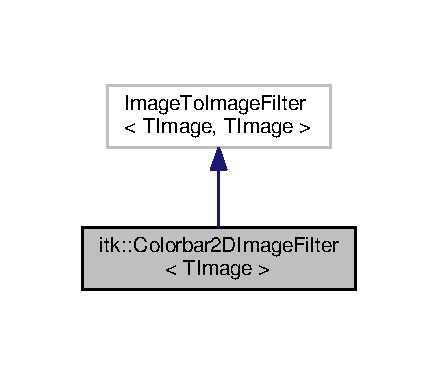
\includegraphics[width=210pt]{classitk_1_1_colorbar2_d_image_filter__inherit__graph}
\end{center}
\end{figure}


Collaboration diagram for itk\-:\-:Colorbar2\-D\-Image\-Filter$<$ T\-Image $>$\-:
\nopagebreak
\begin{figure}[H]
\begin{center}
\leavevmode
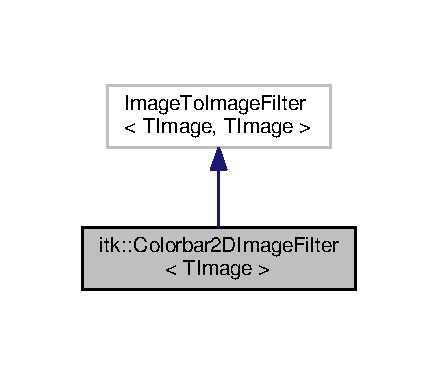
\includegraphics[width=210pt]{classitk_1_1_colorbar2_d_image_filter__coll__graph}
\end{center}
\end{figure}
\subsection*{Public Types}
\begin{DoxyCompactItemize}
\item 
typedef \hyperlink{classitk_1_1_colorbar2_d_image_filter}{Colorbar2\-D\-Image\-Filter} \hyperlink{classitk_1_1_colorbar2_d_image_filter_a2c93d9d0cfe2be77c3f86bf7c9526c34}{Self}
\item 
\hypertarget{classitk_1_1_colorbar2_d_image_filter_a5e77f2c1678f5a62d635afa7077c227f}{typedef Image\-To\-Image\-Filter\\*
$<$ T\-Image, T\-Image $>$ {\bfseries Superclass}}\label{classitk_1_1_colorbar2_d_image_filter_a5e77f2c1678f5a62d635afa7077c227f}

\item 
\hypertarget{classitk_1_1_colorbar2_d_image_filter_a31bbb4eebad609e9dfca8f87a69a70ad}{typedef Smart\-Pointer$<$ \hyperlink{classitk_1_1_colorbar2_d_image_filter_a2c93d9d0cfe2be77c3f86bf7c9526c34}{Self} $>$ {\bfseries Pointer}}\label{classitk_1_1_colorbar2_d_image_filter_a31bbb4eebad609e9dfca8f87a69a70ad}

\item 
\hypertarget{classitk_1_1_colorbar2_d_image_filter_a9cf8e325a86cac28dc661647905381f9}{typedef T\-Image\-::\-Pixel\-Type {\bfseries Pixel\-Type\-In}}\label{classitk_1_1_colorbar2_d_image_filter_a9cf8e325a86cac28dc661647905381f9}

\item 
\hypertarget{classitk_1_1_colorbar2_d_image_filter_acb0402b76750a2b5f895e5f1ca0e56c0}{typedef T\-Image\-::\-Pixel\-Type {\bfseries Pixel\-Type\-Out}}\label{classitk_1_1_colorbar2_d_image_filter_acb0402b76750a2b5f895e5f1ca0e56c0}

\end{DoxyCompactItemize}
\subsection*{Public Member Functions}
\begin{DoxyCompactItemize}
\item 
\hyperlink{classitk_1_1_colorbar2_d_image_filter_abd868d4b97128f6fd9373bc4929792e6}{itk\-New\-Macro} (\hyperlink{classitk_1_1_colorbar2_d_image_filter_a2c93d9d0cfe2be77c3f86bf7c9526c34}{Self})
\item 
\hyperlink{classitk_1_1_colorbar2_d_image_filter_ace645ca59853c18b7c077c2c852b3712}{itk\-Type\-Macro} (Ox\-Colorbar\-Image\-Filter, Image\-To\-Image\-Filter)
\end{DoxyCompactItemize}
\subsection*{Protected Member Functions}
\begin{DoxyCompactItemize}
\item 
\hyperlink{classitk_1_1_colorbar2_d_image_filter_ae103d71eaad083a9303743ee0789457f}{Colorbar2\-D\-Image\-Filter} ()
\item 
\hyperlink{classitk_1_1_colorbar2_d_image_filter_ae2fca5a6a90a6d3dc4ab6f1ae569be9c}{$\sim$\-Colorbar2\-D\-Image\-Filter} ()
\item 
virtual void \hyperlink{classitk_1_1_colorbar2_d_image_filter_aeddf7656f339c33f2412bc222db4d558}{Generate\-Data} () I\-T\-K\-\_\-\-O\-V\-E\-R\-R\-I\-D\-E
\end{DoxyCompactItemize}


\subsection{Detailed Description}
\subsubsection*{template$<$typename T\-Image$>$class itk\-::\-Colorbar2\-D\-Image\-Filter$<$ T\-Image $>$}


\begin{DoxyTemplParams}{Template Parameters}
{\em T\-Image} & \\
\hline
\end{DoxyTemplParams}


\subsection{Member Typedef Documentation}
\hypertarget{classitk_1_1_colorbar2_d_image_filter_a2c93d9d0cfe2be77c3f86bf7c9526c34}{\index{itk\-::\-Colorbar2\-D\-Image\-Filter@{itk\-::\-Colorbar2\-D\-Image\-Filter}!Self@{Self}}
\index{Self@{Self}!itk::Colorbar2DImageFilter@{itk\-::\-Colorbar2\-D\-Image\-Filter}}
\subsubsection[{Self}]{\setlength{\rightskip}{0pt plus 5cm}template$<$typename T\-Image $>$ typedef {\bf Colorbar2\-D\-Image\-Filter} {\bf itk\-::\-Colorbar2\-D\-Image\-Filter}$<$ T\-Image $>$\-::{\bf Self}}}\label{classitk_1_1_colorbar2_d_image_filter_a2c93d9d0cfe2be77c3f86bf7c9526c34}
Standard class typedefs. 

\subsection{Constructor \& Destructor Documentation}
\hypertarget{classitk_1_1_colorbar2_d_image_filter_ae103d71eaad083a9303743ee0789457f}{\index{itk\-::\-Colorbar2\-D\-Image\-Filter@{itk\-::\-Colorbar2\-D\-Image\-Filter}!Colorbar2\-D\-Image\-Filter@{Colorbar2\-D\-Image\-Filter}}
\index{Colorbar2\-D\-Image\-Filter@{Colorbar2\-D\-Image\-Filter}!itk::Colorbar2DImageFilter@{itk\-::\-Colorbar2\-D\-Image\-Filter}}
\subsubsection[{Colorbar2\-D\-Image\-Filter}]{\setlength{\rightskip}{0pt plus 5cm}template$<$typename T\-Image $>$ {\bf itk\-::\-Colorbar2\-D\-Image\-Filter}$<$ T\-Image $>$\-::{\bf Colorbar2\-D\-Image\-Filter} (
\begin{DoxyParamCaption}
{}
\end{DoxyParamCaption}
)\hspace{0.3cm}{\ttfamily [inline]}, {\ttfamily [protected]}}}\label{classitk_1_1_colorbar2_d_image_filter_ae103d71eaad083a9303743ee0789457f}
Constructor. \hypertarget{classitk_1_1_colorbar2_d_image_filter_ae2fca5a6a90a6d3dc4ab6f1ae569be9c}{\index{itk\-::\-Colorbar2\-D\-Image\-Filter@{itk\-::\-Colorbar2\-D\-Image\-Filter}!$\sim$\-Colorbar2\-D\-Image\-Filter@{$\sim$\-Colorbar2\-D\-Image\-Filter}}
\index{$\sim$\-Colorbar2\-D\-Image\-Filter@{$\sim$\-Colorbar2\-D\-Image\-Filter}!itk::Colorbar2DImageFilter@{itk\-::\-Colorbar2\-D\-Image\-Filter}}
\subsubsection[{$\sim$\-Colorbar2\-D\-Image\-Filter}]{\setlength{\rightskip}{0pt plus 5cm}template$<$typename T\-Image $>$ {\bf itk\-::\-Colorbar2\-D\-Image\-Filter}$<$ T\-Image $>$\-::$\sim${\bf Colorbar2\-D\-Image\-Filter} (
\begin{DoxyParamCaption}
{}
\end{DoxyParamCaption}
)\hspace{0.3cm}{\ttfamily [inline]}, {\ttfamily [protected]}}}\label{classitk_1_1_colorbar2_d_image_filter_ae2fca5a6a90a6d3dc4ab6f1ae569be9c}
Destructor. 

\subsection{Member Function Documentation}
\hypertarget{classitk_1_1_colorbar2_d_image_filter_aeddf7656f339c33f2412bc222db4d558}{\index{itk\-::\-Colorbar2\-D\-Image\-Filter@{itk\-::\-Colorbar2\-D\-Image\-Filter}!Generate\-Data@{Generate\-Data}}
\index{Generate\-Data@{Generate\-Data}!itk::Colorbar2DImageFilter@{itk\-::\-Colorbar2\-D\-Image\-Filter}}
\subsubsection[{Generate\-Data}]{\setlength{\rightskip}{0pt plus 5cm}template$<$typename T\-Image $>$ virtual void {\bf itk\-::\-Colorbar2\-D\-Image\-Filter}$<$ T\-Image $>$\-::Generate\-Data (
\begin{DoxyParamCaption}
{}
\end{DoxyParamCaption}
)\hspace{0.3cm}{\ttfamily [protected]}, {\ttfamily [virtual]}}}\label{classitk_1_1_colorbar2_d_image_filter_aeddf7656f339c33f2412bc222db4d558}
Does the real work. \hypertarget{classitk_1_1_colorbar2_d_image_filter_abd868d4b97128f6fd9373bc4929792e6}{\index{itk\-::\-Colorbar2\-D\-Image\-Filter@{itk\-::\-Colorbar2\-D\-Image\-Filter}!itk\-New\-Macro@{itk\-New\-Macro}}
\index{itk\-New\-Macro@{itk\-New\-Macro}!itk::Colorbar2DImageFilter@{itk\-::\-Colorbar2\-D\-Image\-Filter}}
\subsubsection[{itk\-New\-Macro}]{\setlength{\rightskip}{0pt plus 5cm}template$<$typename T\-Image $>$ {\bf itk\-::\-Colorbar2\-D\-Image\-Filter}$<$ T\-Image $>$\-::itk\-New\-Macro (
\begin{DoxyParamCaption}
\item[{{\bf Self}}]{}
\end{DoxyParamCaption}
)}}\label{classitk_1_1_colorbar2_d_image_filter_abd868d4b97128f6fd9373bc4929792e6}
Method for creation through the object factory. \hypertarget{classitk_1_1_colorbar2_d_image_filter_ace645ca59853c18b7c077c2c852b3712}{\index{itk\-::\-Colorbar2\-D\-Image\-Filter@{itk\-::\-Colorbar2\-D\-Image\-Filter}!itk\-Type\-Macro@{itk\-Type\-Macro}}
\index{itk\-Type\-Macro@{itk\-Type\-Macro}!itk::Colorbar2DImageFilter@{itk\-::\-Colorbar2\-D\-Image\-Filter}}
\subsubsection[{itk\-Type\-Macro}]{\setlength{\rightskip}{0pt plus 5cm}template$<$typename T\-Image $>$ {\bf itk\-::\-Colorbar2\-D\-Image\-Filter}$<$ T\-Image $>$\-::itk\-Type\-Macro (
\begin{DoxyParamCaption}
\item[{Ox\-Colorbar\-Image\-Filter}]{, }
\item[{Image\-To\-Image\-Filter}]{}
\end{DoxyParamCaption}
)}}\label{classitk_1_1_colorbar2_d_image_filter_ace645ca59853c18b7c077c2c852b3712}
Run-\/time type information (and related methods). 

The documentation for this class was generated from the following file\-:\begin{DoxyCompactItemize}
\item 
lib/itk\-Colorbar2\-D\-Image\-Filter.\-h\end{DoxyCompactItemize}

\hypertarget{class_ox_1_1_factory_of_calculators}{}\section{Ox\+:\+:Factory\+Of\+Calculators$<$ T\+Y\+PE $>$ Class Template Reference}
\label{class_ox_1_1_factory_of_calculators}\index{Ox\+::\+Factory\+Of\+Calculators$<$ T\+Y\+P\+E $>$@{Ox\+::\+Factory\+Of\+Calculators$<$ T\+Y\+P\+E $>$}}
\subsection*{Static Public Member Functions}
\begin{DoxyCompactItemize}
\item 
static \hyperlink{class_ox_1_1_calculator}{Calculator}$<$ T\+Y\+PE $>$ $\ast$ {\bfseries new\+By\+Factory} (\hyperlink{class_ox_1_1_tomato_options}{Tomato\+Options}$<$ T\+Y\+PE $>$ $\ast$opts)\hypertarget{class_ox_1_1_factory_of_calculators_a43c28f519cc510bc1c8d1a86b14512b4}{}\label{class_ox_1_1_factory_of_calculators_a43c28f519cc510bc1c8d1a86b14512b4}

\item 
static void {\bfseries disp} (int parameter\+\_\+to\+\_\+map=-\/1)\hypertarget{class_ox_1_1_factory_of_calculators_a80052ba880fca49a529c839b33927b21}{}\label{class_ox_1_1_factory_of_calculators_a80052ba880fca49a529c839b33927b21}

\end{DoxyCompactItemize}


The documentation for this class was generated from the following files\+:\begin{DoxyCompactItemize}
\item 
lib/\hyperlink{_ox_factory_of_calculators_8h}{Ox\+Factory\+Of\+Calculators.\+h}\item 
lib/\hyperlink{_ox_factory_of_calculators_8hxx}{Ox\+Factory\+Of\+Calculators.\+hxx}\end{DoxyCompactItemize}

\hypertarget{class_ox_1_1_factory_of_fitters}{\section{Ox\-:\-:Factory\-Of\-Fitters$<$ T\-Y\-P\-E $>$ Class Template Reference}
\label{class_ox_1_1_factory_of_fitters}\index{Ox\-::\-Factory\-Of\-Fitters$<$ T\-Y\-P\-E $>$@{Ox\-::\-Factory\-Of\-Fitters$<$ T\-Y\-P\-E $>$}}
}
\subsection*{Static Public Member Functions}
\begin{DoxyCompactItemize}
\item 
\hypertarget{class_ox_1_1_factory_of_fitters_aeec858b4bf98eb6f7915ead00c3ede10}{static \hyperlink{class_ox_1_1_fitter}{Fitter}$<$ T\-Y\-P\-E $>$ $\ast$ {\bfseries new\-By\-Factory} (\hyperlink{struct_ox_1_1_tomato_options}{Tomato\-Options}$<$ T\-Y\-P\-E $>$ $\ast$opts)}\label{class_ox_1_1_factory_of_fitters_aeec858b4bf98eb6f7915ead00c3ede10}

\end{DoxyCompactItemize}


The documentation for this class was generated from the following file\-:\begin{DoxyCompactItemize}
\item 
app/\hyperlink{_ox_factory_of_fitters_8h}{Ox\-Factory\-Of\-Fitters.\-h}\end{DoxyCompactItemize}

\hypertarget{class_ox_1_1_factory_of_functions}{\section{Ox\-:\-:Factory\-Of\-Functions$<$ T\-Y\-P\-E $>$ Class Template Reference}
\label{class_ox_1_1_factory_of_functions}\index{Ox\-::\-Factory\-Of\-Functions$<$ T\-Y\-P\-E $>$@{Ox\-::\-Factory\-Of\-Functions$<$ T\-Y\-P\-E $>$}}
}
\subsection*{Static Public Member Functions}
\begin{DoxyCompactItemize}
\item 
\hypertarget{class_ox_1_1_factory_of_functions_a188a9a0d61fcbca185c90e548be71bf0}{static \hyperlink{class_ox_1_1_functions_t1}{Functions\-T1}$<$ T\-Y\-P\-E $>$ $\ast$ {\bfseries new\-By\-Factory} (\hyperlink{struct_ox_1_1_tomato_options}{Tomato\-Options}$<$ T\-Y\-P\-E $>$ $\ast$opts)}\label{class_ox_1_1_factory_of_functions_a188a9a0d61fcbca185c90e548be71bf0}

\end{DoxyCompactItemize}


The documentation for this class was generated from the following file\-:\begin{DoxyCompactItemize}
\item 
app/\hyperlink{_ox_factory_of_functions_8h}{Ox\-Factory\-Of\-Functions.\-h}\end{DoxyCompactItemize}

\hypertarget{class_ox_1_1_factory_of_sign_calculators}{\section{Ox\-:\-:Factory\-Of\-Sign\-Calculators$<$ T\-Y\-P\-E $>$ Class Template Reference}
\label{class_ox_1_1_factory_of_sign_calculators}\index{Ox\-::\-Factory\-Of\-Sign\-Calculators$<$ T\-Y\-P\-E $>$@{Ox\-::\-Factory\-Of\-Sign\-Calculators$<$ T\-Y\-P\-E $>$}}
}
\subsection*{Static Public Member Functions}
\begin{DoxyCompactItemize}
\item 
\hypertarget{class_ox_1_1_factory_of_sign_calculators_a1241354771109d5dbd3ffb3d6ec817a3}{static \hyperlink{class_ox_1_1_sign_calculator}{Sign\-Calculator}$<$ T\-Y\-P\-E $>$ $\ast$ {\bfseries new\-By\-Factory} (\hyperlink{struct_ox_1_1_tomato_options}{Tomato\-Options}$<$ T\-Y\-P\-E $>$ $\ast$opts)}\label{class_ox_1_1_factory_of_sign_calculators_a1241354771109d5dbd3ffb3d6ec817a3}

\item 
\hypertarget{class_ox_1_1_factory_of_sign_calculators_a1230de323f020ee2f5bef7d93636c6f2}{static void {\bfseries disp} (int sign\-\_\-calc\-\_\-method=-\/1)}\label{class_ox_1_1_factory_of_sign_calculators_a1230de323f020ee2f5bef7d93636c6f2}

\end{DoxyCompactItemize}


The documentation for this class was generated from the following files\-:\begin{DoxyCompactItemize}
\item 
lib/\hyperlink{_ox_factory_of_sign_calculators_8h}{Ox\-Factory\-Of\-Sign\-Calculators.\-h}\item 
lib/\hyperlink{_ox_factory_of_sign_calculators_8hxx}{Ox\-Factory\-Of\-Sign\-Calculators.\-hxx}\end{DoxyCompactItemize}

\hypertarget{class_ox_1_1_factory_of_start_point_calculators}{\section{Ox\-:\-:Factory\-Of\-Start\-Point\-Calculators$<$ T\-Y\-P\-E $>$ Class Template Reference}
\label{class_ox_1_1_factory_of_start_point_calculators}\index{Ox\-::\-Factory\-Of\-Start\-Point\-Calculators$<$ T\-Y\-P\-E $>$@{Ox\-::\-Factory\-Of\-Start\-Point\-Calculators$<$ T\-Y\-P\-E $>$}}
}
\subsection*{Static Public Member Functions}
\begin{DoxyCompactItemize}
\item 
\hypertarget{class_ox_1_1_factory_of_start_point_calculators_a49529379f7de8796134663b95277cdb0}{static \hyperlink{class_ox_1_1_start_point_calculator}{Start\-Point\-Calculator}\\*
$<$ T\-Y\-P\-E $>$ $\ast$ {\bfseries new\-By\-Factory} (\hyperlink{struct_ox_1_1_ox_shmolli2_options}{Ox\-Shmolli2\-Options}$<$ T\-Y\-P\-E $>$ $\ast$opts)}\label{class_ox_1_1_factory_of_start_point_calculators_a49529379f7de8796134663b95277cdb0}

\end{DoxyCompactItemize}


The documentation for this class was generated from the following file\-:\begin{DoxyCompactItemize}
\item 
app/\hyperlink{_ox_factory_of_start_point_calculators_8h}{Ox\-Factory\-Of\-Start\-Point\-Calculators.\-h}\end{DoxyCompactItemize}

\hypertarget{class_ox_1_1_fitter}{}\section{Ox\+:\+:Fitter$<$ Measure\+Type $>$ Class Template Reference}
\label{class_ox_1_1_fitter}\index{Ox\+::\+Fitter$<$ Measure\+Type $>$@{Ox\+::\+Fitter$<$ Measure\+Type $>$}}


{\ttfamily \#include $<$Ox\+Fitter.\+h$>$}

\subsection*{Public Member Functions}
\begin{DoxyCompactItemize}
\item 
virtual int \hyperlink{class_ox_1_1_fitter_a8f240f0da86d06b339ab2747e87f21b9}{perform\+Fitting} ()=0
\item 
virtual const \hyperlink{class_ox_1_1_model}{Model}$<$ Measure\+Type $>$ $\ast$ {\bfseries get\+Model} () const \hypertarget{class_ox_1_1_fitter_aab3e83fef361dc2dfa855c4988af2393}{}\label{class_ox_1_1_fitter_aab3e83fef361dc2dfa855c4988af2393}

\item 
virtual Measure\+Type $\ast$ {\bfseries get\+Parameters} ()\hypertarget{class_ox_1_1_fitter_a5e87dd37738745f98d904865f6b89219}{}\label{class_ox_1_1_fitter_a5e87dd37738745f98d904865f6b89219}

\item 
virtual Measure\+Type {\bfseries get\+Mse} () const \hypertarget{class_ox_1_1_fitter_ade772dbac027c450451fc6845ce710f5}{}\label{class_ox_1_1_fitter_ade772dbac027c450451fc6845ce710f5}

\item 
virtual const Measure\+Type {\bfseries get\+X\+Tolerance} () const \hypertarget{class_ox_1_1_fitter_a21f92547f664c9b6f3fa8da4c7d16965}{}\label{class_ox_1_1_fitter_a21f92547f664c9b6f3fa8da4c7d16965}

\item 
virtual const Measure\+Type {\bfseries get\+F\+Tolerance} () const \hypertarget{class_ox_1_1_fitter_ac62bf275718aafc95b5e49d0aa9fc1ef}{}\label{class_ox_1_1_fitter_ac62bf275718aafc95b5e49d0aa9fc1ef}

\item 
virtual const bool {\bfseries get\+Use\+Gradient} () const \hypertarget{class_ox_1_1_fitter_aba3fc8ad5260390faf59e2f904ab6d6d}{}\label{class_ox_1_1_fitter_aba3fc8ad5260390faf59e2f904ab6d6d}

\item 
virtual const unsigned int {\bfseries get\+Max\+Function\+Evals} () const \hypertarget{class_ox_1_1_fitter_a04f36e075f86c6a89df833d17b9f029d}{}\label{class_ox_1_1_fitter_a04f36e075f86c6a89df833d17b9f029d}

\item 
virtual const unsigned int {\bfseries get\+Thread\+Id} () const \hypertarget{class_ox_1_1_fitter_a68e317f1c05ea2aa24f9d4803ee19215}{}\label{class_ox_1_1_fitter_a68e317f1c05ea2aa24f9d4803ee19215}

\item 
virtual const bool {\bfseries get\+Verbose} () const \hypertarget{class_ox_1_1_fitter_afeba16a2218db1f3fc646e2dde75f386}{}\label{class_ox_1_1_fitter_afeba16a2218db1f3fc646e2dde75f386}

\item 
virtual const bool {\bfseries get\+Trace} () const \hypertarget{class_ox_1_1_fitter_a9c3401372be5c8698464deb05c0f5533}{}\label{class_ox_1_1_fitter_a9c3401372be5c8698464deb05c0f5533}

\item 
virtual void {\bfseries set\+Model} (\hyperlink{class_ox_1_1_model}{Model}$<$ Measure\+Type $>$ $\ast$\+\_\+\+Model\+T1)\hypertarget{class_ox_1_1_fitter_a58bc5939283a694d4683dcc160ad4009}{}\label{class_ox_1_1_fitter_a58bc5939283a694d4683dcc160ad4009}

\item 
virtual void {\bfseries set\+Parameters} (Measure\+Type $\ast$\+\_\+\+Parameters)\hypertarget{class_ox_1_1_fitter_ab97f65c7d4d4db9bb0f5934aa0601b73}{}\label{class_ox_1_1_fitter_ab97f65c7d4d4db9bb0f5934aa0601b73}

\item 
virtual void {\bfseries set\+Mse} (Measure\+Type mse)\hypertarget{class_ox_1_1_fitter_a6a76eaeb797c09b75b9c0c3cd6ed326b}{}\label{class_ox_1_1_fitter_a6a76eaeb797c09b75b9c0c3cd6ed326b}

\item 
virtual void {\bfseries set\+X\+Tolerance} (const Measure\+Type \+\_\+\+X\+Tolerance)\hypertarget{class_ox_1_1_fitter_ad2b680ee88b12dd51538a2da865b2589}{}\label{class_ox_1_1_fitter_ad2b680ee88b12dd51538a2da865b2589}

\item 
virtual void {\bfseries set\+Use\+Gradient} (const bool \+\_\+\+Use\+Gradient)\hypertarget{class_ox_1_1_fitter_a2441247888adc90a26d779043f10c5e1}{}\label{class_ox_1_1_fitter_a2441247888adc90a26d779043f10c5e1}

\item 
virtual void {\bfseries set\+F\+Tolerance} (const Measure\+Type \+\_\+\+F\+Tolerance)\hypertarget{class_ox_1_1_fitter_aca7109a663e737c46cb29483c2276f4a}{}\label{class_ox_1_1_fitter_aca7109a663e737c46cb29483c2276f4a}

\item 
virtual void {\bfseries set\+Max\+Function\+Evals} (const unsigned int \+\_\+\+Max\+Function\+Evals)\hypertarget{class_ox_1_1_fitter_a293d2876b8b053bd637c35c3f6f3f68e}{}\label{class_ox_1_1_fitter_a293d2876b8b053bd637c35c3f6f3f68e}

\item 
virtual void {\bfseries set\+Thread\+Id} (const unsigned int \+\_\+\+Thread\+Id)\hypertarget{class_ox_1_1_fitter_aa1fc4674aa6a3e6c8567c86ec1fa90e0}{}\label{class_ox_1_1_fitter_aa1fc4674aa6a3e6c8567c86ec1fa90e0}

\item 
virtual void {\bfseries set\+Verbose} (const bool \+\_\+\+Verbose)\hypertarget{class_ox_1_1_fitter_a696da03b83fe3083f29ae4c0e2ecfc44}{}\label{class_ox_1_1_fitter_a696da03b83fe3083f29ae4c0e2ecfc44}

\item 
virtual void {\bfseries set\+Trace} (const bool \+\_\+\+Trace)\hypertarget{class_ox_1_1_fitter_a4ac0096f6bc6d733c542d28a839d32c9}{}\label{class_ox_1_1_fitter_a4ac0096f6bc6d733c542d28a839d32c9}

\item 
virtual void \hyperlink{class_ox_1_1_fitter_a783ba791c88d7208deb4004354b10022}{copy\+To\+Parameters} (const Measure\+Type $\ast$ptr\+From)
\item 
virtual void \hyperlink{class_ox_1_1_fitter_a0a9b45eb21ba174327f95a894e6331b6}{disp} ()\hypertarget{class_ox_1_1_fitter_a0a9b45eb21ba174327f95a894e6331b6}{}\label{class_ox_1_1_fitter_a0a9b45eb21ba174327f95a894e6331b6}

\begin{DoxyCompactList}\small\item\em show me your \hyperlink{class_ox_1_1_fitter}{Fitter} \end{DoxyCompactList}\item 
\hyperlink{class_ox_1_1_fitter_a7b42acb389394bc4c496990eea8b9ac9}{Fitter} ()\hypertarget{class_ox_1_1_fitter_a7b42acb389394bc4c496990eea8b9ac9}{}\label{class_ox_1_1_fitter_a7b42acb389394bc4c496990eea8b9ac9}

\begin{DoxyCompactList}\small\item\em constructor \end{DoxyCompactList}\item 
\hyperlink{class_ox_1_1_fitter_ac51130b722159f88a0dad59877b76417}{Fitter} (const \hyperlink{class_ox_1_1_fitter}{Fitter} \&old)
\item 
virtual \hyperlink{class_ox_1_1_fitter}{Fitter}$<$ Measure\+Type $>$ $\ast$ \hyperlink{class_ox_1_1_fitter_a665ec51e52ed351c9ef801acc83fbdea}{new\+By\+Cloning} ()=0
\item 
virtual \hyperlink{class_ox_1_1_fitter_ab56eef37096f6f0687d83b8d15e00d43}{$\sim$\+Fitter} ()\hypertarget{class_ox_1_1_fitter_ab56eef37096f6f0687d83b8d15e00d43}{}\label{class_ox_1_1_fitter_ab56eef37096f6f0687d83b8d15e00d43}

\begin{DoxyCompactList}\small\item\em do not forget about the virtual destructor, see \href{https://stackoverflow.com/questions/461203/when-to-use-virtual-destructors}{\tt https\+://stackoverflow.\+com/questions/461203/when-\/to-\/use-\/virtual-\/destructors} \end{DoxyCompactList}\end{DoxyCompactItemize}
\subsection*{Protected Attributes}
\begin{DoxyCompactItemize}
\item 
\hyperlink{class_ox_1_1_model}{Model}$<$ Measure\+Type $>$ $\ast$ {\bfseries \+\_\+\+Model}\hypertarget{class_ox_1_1_fitter_ae5a2d2967fb117386a4b73123f188213}{}\label{class_ox_1_1_fitter_ae5a2d2967fb117386a4b73123f188213}

\item 
Measure\+Type $\ast$ {\bfseries \+\_\+\+Parameters}\hypertarget{class_ox_1_1_fitter_a508e5654aaf79dd744ec816d95b7e33c}{}\label{class_ox_1_1_fitter_a508e5654aaf79dd744ec816d95b7e33c}

\item 
Measure\+Type {\bfseries \+\_\+\+Mse}\hypertarget{class_ox_1_1_fitter_a1c5f4e7fa0764489e30685f47fe53190}{}\label{class_ox_1_1_fitter_a1c5f4e7fa0764489e30685f47fe53190}

\item 
Measure\+Type {\bfseries \+\_\+\+X\+Tolerance}\hypertarget{class_ox_1_1_fitter_af91a5ea8fb20072277ddcd64f5537b09}{}\label{class_ox_1_1_fitter_af91a5ea8fb20072277ddcd64f5537b09}

\item 
Measure\+Type {\bfseries \+\_\+\+F\+Tolerance}\hypertarget{class_ox_1_1_fitter_a926f6cf38998f041c31b079e93bf27ab}{}\label{class_ox_1_1_fitter_a926f6cf38998f041c31b079e93bf27ab}

\item 
unsigned int {\bfseries \+\_\+\+Max\+Function\+Evals}\hypertarget{class_ox_1_1_fitter_a3be7ea1c1f19d3f4fb384474e2b1a033}{}\label{class_ox_1_1_fitter_a3be7ea1c1f19d3f4fb384474e2b1a033}

\item 
bool {\bfseries \+\_\+\+Use\+Gradient}\hypertarget{class_ox_1_1_fitter_a34c039e87d52c28b19092535a171264f}{}\label{class_ox_1_1_fitter_a34c039e87d52c28b19092535a171264f}

\item 
unsigned int {\bfseries \+\_\+\+Thread\+Id}\hypertarget{class_ox_1_1_fitter_a0d97d7a9c9fad0349484151464fefe4f}{}\label{class_ox_1_1_fitter_a0d97d7a9c9fad0349484151464fefe4f}

\item 
bool {\bfseries \+\_\+\+Verbose}\hypertarget{class_ox_1_1_fitter_a6457339f5252c85d7c92f20439544975}{}\label{class_ox_1_1_fitter_a6457339f5252c85d7c92f20439544975}

\item 
bool {\bfseries \+\_\+\+Trace}\hypertarget{class_ox_1_1_fitter_a9ba79cb05ecc670254b3e7ddafc519ab}{}\label{class_ox_1_1_fitter_a9ba79cb05ecc670254b3e7ddafc519ab}

\end{DoxyCompactItemize}


\subsection{Detailed Description}
\subsubsection*{template$<$typename Measure\+Type$>$\\*
class Ox\+::\+Fitter$<$ Measure\+Type $>$}


\begin{DoxyTemplParams}{Template Parameters}
{\em Measure\+Type} & \\
\hline
\end{DoxyTemplParams}


\subsection{Constructor \& Destructor Documentation}
\index{Ox\+::\+Fitter@{Ox\+::\+Fitter}!Fitter@{Fitter}}
\index{Fitter@{Fitter}!Ox\+::\+Fitter@{Ox\+::\+Fitter}}
\subsubsection[{\texorpdfstring{Fitter(const Fitter \&old)}{Fitter(const Fitter &old)}}]{\setlength{\rightskip}{0pt plus 5cm}template$<$typename Measure\+Type$>$ {\bf Ox\+::\+Fitter}$<$ Measure\+Type $>$\+::{\bf Fitter} (
\begin{DoxyParamCaption}
\item[{const {\bf Fitter}$<$ Measure\+Type $>$ \&}]{old}
\end{DoxyParamCaption}
)\hspace{0.3cm}{\ttfamily [inline]}}\hypertarget{class_ox_1_1_fitter_ac51130b722159f88a0dad59877b76417}{}\label{class_ox_1_1_fitter_ac51130b722159f88a0dad59877b76417}
copy constructor 
\begin{DoxyParams}{Parameters}
{\em old} & \\
\hline
\end{DoxyParams}


\subsection{Member Function Documentation}
\index{Ox\+::\+Fitter@{Ox\+::\+Fitter}!copy\+To\+Parameters@{copy\+To\+Parameters}}
\index{copy\+To\+Parameters@{copy\+To\+Parameters}!Ox\+::\+Fitter@{Ox\+::\+Fitter}}
\subsubsection[{\texorpdfstring{copy\+To\+Parameters(const Measure\+Type $\ast$ptr\+From)}{copyToParameters(const MeasureType *ptrFrom)}}]{\setlength{\rightskip}{0pt plus 5cm}template$<$typename Measure\+Type$>$ virtual void {\bf Ox\+::\+Fitter}$<$ Measure\+Type $>$\+::copy\+To\+Parameters (
\begin{DoxyParamCaption}
\item[{const Measure\+Type $\ast$}]{ptr\+From}
\end{DoxyParamCaption}
)\hspace{0.3cm}{\ttfamily [inline]}, {\ttfamily [virtual]}}\hypertarget{class_ox_1_1_fitter_a783ba791c88d7208deb4004354b10022}{}\label{class_ox_1_1_fitter_a783ba791c88d7208deb4004354b10022}
copy from ptr\+From to the parameters. Parameters have to be allocated first 
\begin{DoxyParams}{Parameters}
{\em ptr\+From} & \\
\hline
\end{DoxyParams}
\index{Ox\+::\+Fitter@{Ox\+::\+Fitter}!new\+By\+Cloning@{new\+By\+Cloning}}
\index{new\+By\+Cloning@{new\+By\+Cloning}!Ox\+::\+Fitter@{Ox\+::\+Fitter}}
\subsubsection[{\texorpdfstring{new\+By\+Cloning()=0}{newByCloning()=0}}]{\setlength{\rightskip}{0pt plus 5cm}template$<$typename Measure\+Type$>$ virtual {\bf Fitter}$<$Measure\+Type$>$$\ast$ {\bf Ox\+::\+Fitter}$<$ Measure\+Type $>$\+::new\+By\+Cloning (
\begin{DoxyParamCaption}
{}
\end{DoxyParamCaption}
)\hspace{0.3cm}{\ttfamily [pure virtual]}}\hypertarget{class_ox_1_1_fitter_a665ec51e52ed351c9ef801acc83fbdea}{}\label{class_ox_1_1_fitter_a665ec51e52ed351c9ef801acc83fbdea}
cloning \begin{DoxyReturn}{Returns}

\end{DoxyReturn}
\index{Ox\+::\+Fitter@{Ox\+::\+Fitter}!perform\+Fitting@{perform\+Fitting}}
\index{perform\+Fitting@{perform\+Fitting}!Ox\+::\+Fitter@{Ox\+::\+Fitter}}
\subsubsection[{\texorpdfstring{perform\+Fitting()=0}{performFitting()=0}}]{\setlength{\rightskip}{0pt plus 5cm}template$<$typename Measure\+Type$>$ virtual int {\bf Ox\+::\+Fitter}$<$ Measure\+Type $>$\+::perform\+Fitting (
\begin{DoxyParamCaption}
{}
\end{DoxyParamCaption}
)\hspace{0.3cm}{\ttfamily [pure virtual]}}\hypertarget{class_ox_1_1_fitter_a8f240f0da86d06b339ab2747e87f21b9}{}\label{class_ox_1_1_fitter_a8f240f0da86d06b339ab2747e87f21b9}
the most important function of this class \begin{DoxyReturn}{Returns}
success/failure 
\end{DoxyReturn}


The documentation for this class was generated from the following file\+:\begin{DoxyCompactItemize}
\item 
lib/\hyperlink{_ox_fitter_8h}{Ox\+Fitter.\+h}\end{DoxyCompactItemize}

\hypertarget{class_ox_1_1_functions_t1}{\section{Ox\-:\-:Functions\-T1$<$ Measure\-Type $>$ Class Template Reference}
\label{class_ox_1_1_functions_t1}\index{Ox\-::\-Functions\-T1$<$ Measure\-Type $>$@{Ox\-::\-Functions\-T1$<$ Measure\-Type $>$}}
}


Container for a model function, cost function and Least-\/\-Squares function. And derivatives.  




{\ttfamily \#include $<$Ox\-Functions\-T1.\-h$>$}



Inheritance diagram for Ox\-:\-:Functions\-T1$<$ Measure\-Type $>$\-:
\nopagebreak
\begin{figure}[H]
\begin{center}
\leavevmode
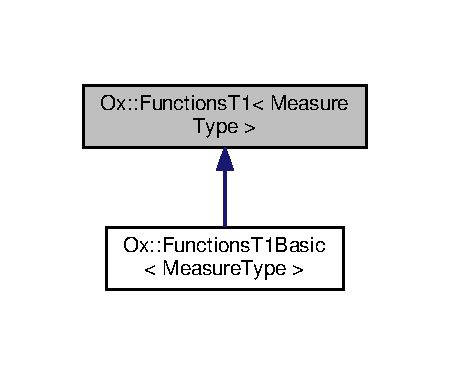
\includegraphics[width=216pt]{class_ox_1_1_functions_t1__inherit__graph}
\end{center}
\end{figure}
\subsection*{Public Member Functions}
\begin{DoxyCompactItemize}
\item 
virtual Measure\-Type \hyperlink{class_ox_1_1_functions_t1_a651f0dca72aab630bc46119094b80aee}{calc\-Model\-Value} (const Measure\-Type $\ast$parameters, Measure\-Type time)=0
\item 
virtual void \hyperlink{class_ox_1_1_functions_t1_ae548ba2f5779aba3d3e37f0bec77e891}{calc\-L\-S\-Residuals} (const Measure\-Type $\ast$parameters, Measure\-Type $\ast$residuals)=0
\item 
virtual Measure\-Type \hyperlink{class_ox_1_1_functions_t1_a70ab239415d72f38bc36cc290fa3b476}{calc\-Cost\-Value} (const Measure\-Type $\ast$parameters)=0
\item 
virtual void \hyperlink{class_ox_1_1_functions_t1_a01df2dd1eb054540eaccfb1dca01c7ce}{calc\-Cost\-Derivative} (const Measure\-Type $\ast$parameters, Measure\-Type $\ast$derivative)=0
\item 
virtual void \hyperlink{class_ox_1_1_functions_t1_a19216f0d9ae8ba2d7cd55df81d370521}{calc\-L\-S\-Jacobian} (const Measure\-Type $\ast$parameters, Measure\-Type $\ast$jacobian)=0
\item 
\hypertarget{class_ox_1_1_functions_t1_a70e137063cc2e6ef086046e596af4a15}{virtual int {\bfseries get\-N\-Samples} ()}\label{class_ox_1_1_functions_t1_a70e137063cc2e6ef086046e596af4a15}

\item 
\hypertarget{class_ox_1_1_functions_t1_a71aafa53236bc1eed5b4d65ae25538c7}{virtual const Measure\-Type $\ast$ {\bfseries get\-Inv\-Times} () const }\label{class_ox_1_1_functions_t1_a71aafa53236bc1eed5b4d65ae25538c7}

\item 
\hypertarget{class_ox_1_1_functions_t1_a73a26e9e37e35c1617a741ad2932bdd8}{virtual const Measure\-Type $\ast$ {\bfseries get\-Echo\-Times} () const }\label{class_ox_1_1_functions_t1_a73a26e9e37e35c1617a741ad2932bdd8}

\item 
\hypertarget{class_ox_1_1_functions_t1_afb89e35bedfd9d608b0afe189d976fa9}{virtual const Measure\-Type $\ast$ {\bfseries get\-Rep\-Times} () const }\label{class_ox_1_1_functions_t1_afb89e35bedfd9d608b0afe189d976fa9}

\item 
\hypertarget{class_ox_1_1_functions_t1_a142aaed9ff99a0dd08460d2581150e9c}{virtual const Measure\-Type $\ast$ {\bfseries get\-Rel\-Acq\-Times} () const }\label{class_ox_1_1_functions_t1_a142aaed9ff99a0dd08460d2581150e9c}

\item 
\hypertarget{class_ox_1_1_functions_t1_adf70d696e9da0fcdb45c4a4d02913d6c}{virtual const Measure\-Type $\ast$ {\bfseries get\-Signal} () const }\label{class_ox_1_1_functions_t1_adf70d696e9da0fcdb45c4a4d02913d6c}

\item 
\hypertarget{class_ox_1_1_functions_t1_a4bd8c56786631568dac07ddae165a6b1}{virtual int {\bfseries get\-N\-Dims} ()}\label{class_ox_1_1_functions_t1_a4bd8c56786631568dac07ddae165a6b1}

\item 
\hypertarget{class_ox_1_1_functions_t1_ac817cab2256c8495bc6979bb1fca2688}{void {\bfseries set\-N\-Samples} (int \-\_\-n\-Samples)}\label{class_ox_1_1_functions_t1_ac817cab2256c8495bc6979bb1fca2688}

\item 
\hypertarget{class_ox_1_1_functions_t1_a5a96e27da44213d1b4f4a7e91d8e0347}{virtual void {\bfseries set\-Inv\-Times} (const Measure\-Type $\ast$\-\_\-\-Inv\-Times)}\label{class_ox_1_1_functions_t1_a5a96e27da44213d1b4f4a7e91d8e0347}

\item 
\hypertarget{class_ox_1_1_functions_t1_a3ce890151e04cf3c9649c1e8bed3dcb1}{virtual void {\bfseries set\-Echo\-Times} (const Measure\-Type $\ast$\-\_\-\-Echo\-Times)}\label{class_ox_1_1_functions_t1_a3ce890151e04cf3c9649c1e8bed3dcb1}

\item 
\hypertarget{class_ox_1_1_functions_t1_ad221400dbedf2ac324f0e80105a261fb}{virtual void {\bfseries set\-Rep\-Times} (const Measure\-Type $\ast$\-\_\-\-Rep\-Times)}\label{class_ox_1_1_functions_t1_ad221400dbedf2ac324f0e80105a261fb}

\item 
\hypertarget{class_ox_1_1_functions_t1_a278e7e3d4989fb9305cdc0ec6160f1a8}{virtual void {\bfseries set\-Rel\-Acq\-Times} (const Measure\-Type $\ast$\-\_\-\-Rel\-Acq\-Times)}\label{class_ox_1_1_functions_t1_a278e7e3d4989fb9305cdc0ec6160f1a8}

\item 
\hypertarget{class_ox_1_1_functions_t1_a73bd06989de4d204d8e654c583cd3ce3}{virtual void {\bfseries set\-Signal} (const Measure\-Type $\ast$\-\_\-\-Signal)}\label{class_ox_1_1_functions_t1_a73bd06989de4d204d8e654c583cd3ce3}

\item 
\hypertarget{class_ox_1_1_functions_t1_a21708a9d44f261ba53648c2e6fcdd3a5}{virtual void \hyperlink{class_ox_1_1_functions_t1_a21708a9d44f261ba53648c2e6fcdd3a5}{disp} ()}\label{class_ox_1_1_functions_t1_a21708a9d44f261ba53648c2e6fcdd3a5}

\begin{DoxyCompactList}\small\item\em show me your \hyperlink{class_ox_1_1_functions_t1}{Functions\-T1} \end{DoxyCompactList}\item 
\hypertarget{class_ox_1_1_functions_t1_a242f775b52419858f76d7711096ac5dc}{void \hyperlink{class_ox_1_1_functions_t1_a242f775b52419858f76d7711096ac5dc}{set\-All\-Pointers\-To\-Null} ()}\label{class_ox_1_1_functions_t1_a242f775b52419858f76d7711096ac5dc}

\begin{DoxyCompactList}\small\item\em set all the pointers to zero \end{DoxyCompactList}\item 
\hypertarget{class_ox_1_1_functions_t1_a7dae9dc71ec97e9eef1308c9937aaaf0}{\hyperlink{class_ox_1_1_functions_t1_a7dae9dc71ec97e9eef1308c9937aaaf0}{Functions\-T1} ()}\label{class_ox_1_1_functions_t1_a7dae9dc71ec97e9eef1308c9937aaaf0}

\begin{DoxyCompactList}\small\item\em constructor \end{DoxyCompactList}\item 
\hyperlink{class_ox_1_1_functions_t1_a8b14d232e9136a64ea3ae8f7a162daad}{Functions\-T1} (const \hyperlink{class_ox_1_1_functions_t1}{Functions\-T1} \&old)
\begin{DoxyCompactList}\small\item\em copy constructor keeps only \-\_\-n\-Samples and \-\_\-n\-Dims \end{DoxyCompactList}\item 
virtual \hyperlink{class_ox_1_1_functions_t1}{Functions\-T1}\\*
$<$ Measure\-Type $>$ $\ast$ \hyperlink{class_ox_1_1_functions_t1_a2246ea540016c650d5a18100697eacb8}{new\-By\-Cloning} ()=0
\item 
\hypertarget{class_ox_1_1_functions_t1_a900d5602b3dd10fca760a304e41da9b5}{virtual \hyperlink{class_ox_1_1_functions_t1_a900d5602b3dd10fca760a304e41da9b5}{$\sim$\-Functions\-T1} ()}\label{class_ox_1_1_functions_t1_a900d5602b3dd10fca760a304e41da9b5}

\begin{DoxyCompactList}\small\item\em do not forget about the virtual destructor, see \href{https://stackoverflow.com/questions/461203/when-to-use-virtual-destructors}{\tt https\-://stackoverflow.\-com/questions/461203/when-\/to-\/use-\/virtual-\/destructors} \end{DoxyCompactList}\end{DoxyCompactItemize}
\subsection*{Protected Attributes}
\begin{DoxyCompactItemize}
\item 
\hypertarget{class_ox_1_1_functions_t1_a4e92c3f06b7ef0327d6625a662db4d1c}{const Measure\-Type $\ast$ {\bfseries \-\_\-\-Inv\-Times}}\label{class_ox_1_1_functions_t1_a4e92c3f06b7ef0327d6625a662db4d1c}

\item 
\hypertarget{class_ox_1_1_functions_t1_adaf6b5335e0014ad37c007a24f150343}{const Measure\-Type $\ast$ {\bfseries \-\_\-\-Echo\-Times}}\label{class_ox_1_1_functions_t1_adaf6b5335e0014ad37c007a24f150343}

\item 
\hypertarget{class_ox_1_1_functions_t1_a719873f2f02b6dcf0ae100f9c9a6884f}{const Measure\-Type $\ast$ {\bfseries \-\_\-\-Rep\-Times}}\label{class_ox_1_1_functions_t1_a719873f2f02b6dcf0ae100f9c9a6884f}

\item 
\hypertarget{class_ox_1_1_functions_t1_abfbc38cf7ea0bbc1b52f48a75f281246}{const Measure\-Type $\ast$ {\bfseries \-\_\-\-Rel\-Acq\-Times}}\label{class_ox_1_1_functions_t1_abfbc38cf7ea0bbc1b52f48a75f281246}

\item 
\hypertarget{class_ox_1_1_functions_t1_a8f87abd26c39fddd3e2b0085e97c6571}{const Measure\-Type $\ast$ {\bfseries \-\_\-\-Signal}}\label{class_ox_1_1_functions_t1_a8f87abd26c39fddd3e2b0085e97c6571}

\item 
\hypertarget{class_ox_1_1_functions_t1_a32038248ea53c223d9d99cd9cee36378}{int {\bfseries \-\_\-n\-Samples}}\label{class_ox_1_1_functions_t1_a32038248ea53c223d9d99cd9cee36378}

\item 
\hypertarget{class_ox_1_1_functions_t1_a4d42b89cb62d20c80e3210b17a692ed1}{int {\bfseries \-\_\-n\-Dims}}\label{class_ox_1_1_functions_t1_a4d42b89cb62d20c80e3210b17a692ed1}

\end{DoxyCompactItemize}


\subsection{Detailed Description}
\subsubsection*{template$<$typename Measure\-Type$>$class Ox\-::\-Functions\-T1$<$ Measure\-Type $>$}

Container for a model function, cost function and Least-\/\-Squares function. And derivatives. 

Here model function is defined -\/ \hyperlink{class_ox_1_1_functions_t1_a651f0dca72aab630bc46119094b80aee}{calc\-Model\-Value()}. Fitting algorithms based on optimisation need a cost function -\/ \hyperlink{class_ox_1_1_functions_t1_a70ab239415d72f38bc36cc290fa3b476}{calc\-Cost\-Value()}. Fitting algorithms based on least squares need a residuals calculation -\/ \hyperlink{class_ox_1_1_functions_t1_ae548ba2f5779aba3d3e37f0bec77e891}{calc\-L\-S\-Residuals()}. Some fitting algorithms use derivatives, hence \hyperlink{class_ox_1_1_functions_t1_a19216f0d9ae8ba2d7cd55df81d370521}{calc\-L\-S\-Jacobian()} and \hyperlink{class_ox_1_1_functions_t1_a01df2dd1eb054540eaccfb1dca01c7ce}{calc\-Cost\-Derivative()}. The memeber variables are pointers to c-\/arrays, we need to know how many samples we want to process. Thats the n\-Samples defined in the constructor. T\-O\-D\-O\-: think about moving \-\_\-\-Parameters out of this class and take it as a parameter of all the above functions 
\begin{DoxyTemplParams}{Template Parameters}
{\em Measure\-Type} & \\
\hline
\end{DoxyTemplParams}


\subsection{Constructor \& Destructor Documentation}
\hypertarget{class_ox_1_1_functions_t1_a8b14d232e9136a64ea3ae8f7a162daad}{\index{Ox\-::\-Functions\-T1@{Ox\-::\-Functions\-T1}!Functions\-T1@{Functions\-T1}}
\index{Functions\-T1@{Functions\-T1}!Ox::FunctionsT1@{Ox\-::\-Functions\-T1}}
\subsubsection[{Functions\-T1}]{\setlength{\rightskip}{0pt plus 5cm}template$<$typename Measure\-Type$>$ {\bf Ox\-::\-Functions\-T1}$<$ Measure\-Type $>$\-::{\bf Functions\-T1} (
\begin{DoxyParamCaption}
\item[{const {\bf Functions\-T1}$<$ Measure\-Type $>$ \&}]{old}
\end{DoxyParamCaption}
)\hspace{0.3cm}{\ttfamily [inline]}}}\label{class_ox_1_1_functions_t1_a8b14d232e9136a64ea3ae8f7a162daad}


copy constructor keeps only \-\_\-n\-Samples and \-\_\-n\-Dims 


\begin{DoxyParams}{Parameters}
{\em old} & \\
\hline
\end{DoxyParams}


\subsection{Member Function Documentation}
\hypertarget{class_ox_1_1_functions_t1_a01df2dd1eb054540eaccfb1dca01c7ce}{\index{Ox\-::\-Functions\-T1@{Ox\-::\-Functions\-T1}!calc\-Cost\-Derivative@{calc\-Cost\-Derivative}}
\index{calc\-Cost\-Derivative@{calc\-Cost\-Derivative}!Ox::FunctionsT1@{Ox\-::\-Functions\-T1}}
\subsubsection[{calc\-Cost\-Derivative}]{\setlength{\rightskip}{0pt plus 5cm}template$<$typename Measure\-Type$>$ virtual void {\bf Ox\-::\-Functions\-T1}$<$ Measure\-Type $>$\-::calc\-Cost\-Derivative (
\begin{DoxyParamCaption}
\item[{const Measure\-Type $\ast$}]{parameters, }
\item[{Measure\-Type $\ast$}]{derivative}
\end{DoxyParamCaption}
)\hspace{0.3cm}{\ttfamily [pure virtual]}}}\label{class_ox_1_1_functions_t1_a01df2dd1eb054540eaccfb1dca01c7ce}
calc\-Cost\-Derivative the most important function of this class 
\begin{DoxyParams}{Parameters}
{\em derivative} & \\
\hline
\end{DoxyParams}


Implemented in \hyperlink{class_ox_1_1_functions_t1_basic_aad13eb43862acead688aeb6781cf8cc7}{Ox\-::\-Functions\-T1\-Basic$<$ Measure\-Type $>$}.

\hypertarget{class_ox_1_1_functions_t1_a70ab239415d72f38bc36cc290fa3b476}{\index{Ox\-::\-Functions\-T1@{Ox\-::\-Functions\-T1}!calc\-Cost\-Value@{calc\-Cost\-Value}}
\index{calc\-Cost\-Value@{calc\-Cost\-Value}!Ox::FunctionsT1@{Ox\-::\-Functions\-T1}}
\subsubsection[{calc\-Cost\-Value}]{\setlength{\rightskip}{0pt plus 5cm}template$<$typename Measure\-Type$>$ virtual Measure\-Type {\bf Ox\-::\-Functions\-T1}$<$ Measure\-Type $>$\-::calc\-Cost\-Value (
\begin{DoxyParamCaption}
\item[{const Measure\-Type $\ast$}]{parameters}
\end{DoxyParamCaption}
)\hspace{0.3cm}{\ttfamily [pure virtual]}}}\label{class_ox_1_1_functions_t1_a70ab239415d72f38bc36cc290fa3b476}
calc\-Cost\-Value the most important function of this class \begin{DoxyReturn}{Returns}

\end{DoxyReturn}


Implemented in \hyperlink{class_ox_1_1_functions_t1_basic_a60dff997b49111dbeb0f76204cb0dc8f}{Ox\-::\-Functions\-T1\-Basic$<$ Measure\-Type $>$}.

\hypertarget{class_ox_1_1_functions_t1_a19216f0d9ae8ba2d7cd55df81d370521}{\index{Ox\-::\-Functions\-T1@{Ox\-::\-Functions\-T1}!calc\-L\-S\-Jacobian@{calc\-L\-S\-Jacobian}}
\index{calc\-L\-S\-Jacobian@{calc\-L\-S\-Jacobian}!Ox::FunctionsT1@{Ox\-::\-Functions\-T1}}
\subsubsection[{calc\-L\-S\-Jacobian}]{\setlength{\rightskip}{0pt plus 5cm}template$<$typename Measure\-Type$>$ virtual void {\bf Ox\-::\-Functions\-T1}$<$ Measure\-Type $>$\-::calc\-L\-S\-Jacobian (
\begin{DoxyParamCaption}
\item[{const Measure\-Type $\ast$}]{parameters, }
\item[{Measure\-Type $\ast$}]{jacobian}
\end{DoxyParamCaption}
)\hspace{0.3cm}{\ttfamily [pure virtual]}}}\label{class_ox_1_1_functions_t1_a19216f0d9ae8ba2d7cd55df81d370521}
calc\-L\-S\-Jacobian the most important function of this class 
\begin{DoxyParams}{Parameters}
{\em jacobian} & -\/ 2d matrix stored as 1d array \\
\hline
\end{DoxyParams}


Implemented in \hyperlink{class_ox_1_1_functions_t1_basic_a8fb79c60d2eaaf8a5d982f4bcddbb21e}{Ox\-::\-Functions\-T1\-Basic$<$ Measure\-Type $>$}.

\hypertarget{class_ox_1_1_functions_t1_ae548ba2f5779aba3d3e37f0bec77e891}{\index{Ox\-::\-Functions\-T1@{Ox\-::\-Functions\-T1}!calc\-L\-S\-Residuals@{calc\-L\-S\-Residuals}}
\index{calc\-L\-S\-Residuals@{calc\-L\-S\-Residuals}!Ox::FunctionsT1@{Ox\-::\-Functions\-T1}}
\subsubsection[{calc\-L\-S\-Residuals}]{\setlength{\rightskip}{0pt plus 5cm}template$<$typename Measure\-Type$>$ virtual void {\bf Ox\-::\-Functions\-T1}$<$ Measure\-Type $>$\-::calc\-L\-S\-Residuals (
\begin{DoxyParamCaption}
\item[{const Measure\-Type $\ast$}]{parameters, }
\item[{Measure\-Type $\ast$}]{residuals}
\end{DoxyParamCaption}
)\hspace{0.3cm}{\ttfamily [pure virtual]}}}\label{class_ox_1_1_functions_t1_ae548ba2f5779aba3d3e37f0bec77e891}
calc\-L\-S\-Residuals the most important function of this class 
\begin{DoxyParams}{Parameters}
{\em residuals} & \\
\hline
\end{DoxyParams}


Implemented in \hyperlink{class_ox_1_1_functions_t1_basic_a2e292dec4a234ed53d6cb33c4a590d9f}{Ox\-::\-Functions\-T1\-Basic$<$ Measure\-Type $>$}.

\hypertarget{class_ox_1_1_functions_t1_a651f0dca72aab630bc46119094b80aee}{\index{Ox\-::\-Functions\-T1@{Ox\-::\-Functions\-T1}!calc\-Model\-Value@{calc\-Model\-Value}}
\index{calc\-Model\-Value@{calc\-Model\-Value}!Ox::FunctionsT1@{Ox\-::\-Functions\-T1}}
\subsubsection[{calc\-Model\-Value}]{\setlength{\rightskip}{0pt plus 5cm}template$<$typename Measure\-Type$>$ virtual Measure\-Type {\bf Ox\-::\-Functions\-T1}$<$ Measure\-Type $>$\-::calc\-Model\-Value (
\begin{DoxyParamCaption}
\item[{const Measure\-Type $\ast$}]{parameters, }
\item[{Measure\-Type}]{time}
\end{DoxyParamCaption}
)\hspace{0.3cm}{\ttfamily [pure virtual]}}}\label{class_ox_1_1_functions_t1_a651f0dca72aab630bc46119094b80aee}
calc\-Model\-Value the most important function of this class 
\begin{DoxyParams}{Parameters}
{\em time} & \\
\hline
\end{DoxyParams}
\begin{DoxyReturn}{Returns}
model(time) 
\end{DoxyReturn}


Implemented in \hyperlink{class_ox_1_1_functions_t1_basic_a86c92d7a622a925f2c0a8f39c93470d8}{Ox\-::\-Functions\-T1\-Basic$<$ Measure\-Type $>$}.

\hypertarget{class_ox_1_1_functions_t1_a2246ea540016c650d5a18100697eacb8}{\index{Ox\-::\-Functions\-T1@{Ox\-::\-Functions\-T1}!new\-By\-Cloning@{new\-By\-Cloning}}
\index{new\-By\-Cloning@{new\-By\-Cloning}!Ox::FunctionsT1@{Ox\-::\-Functions\-T1}}
\subsubsection[{new\-By\-Cloning}]{\setlength{\rightskip}{0pt plus 5cm}template$<$typename Measure\-Type$>$ virtual {\bf Functions\-T1}$<$Measure\-Type$>$$\ast$ {\bf Ox\-::\-Functions\-T1}$<$ Measure\-Type $>$\-::new\-By\-Cloning (
\begin{DoxyParamCaption}
{}
\end{DoxyParamCaption}
)\hspace{0.3cm}{\ttfamily [pure virtual]}}}\label{class_ox_1_1_functions_t1_a2246ea540016c650d5a18100697eacb8}
cloning \begin{DoxyReturn}{Returns}

\end{DoxyReturn}


Implemented in \hyperlink{class_ox_1_1_functions_t1_basic_a0bceaf2c2b424cfa2366d943d92814e3}{Ox\-::\-Functions\-T1\-Basic$<$ Measure\-Type $>$}.



The documentation for this class was generated from the following file\-:\begin{DoxyCompactItemize}
\item 
lib/\hyperlink{_ox_functions_t1_8h}{Ox\-Functions\-T1.\-h}\end{DoxyCompactItemize}

\hypertarget{class_ox_1_1_functions_t1_basic}{\section{Ox\-:\-:Functions\-T1\-Basic$<$ Measure\-Type $>$ Class Template Reference}
\label{class_ox_1_1_functions_t1_basic}\index{Ox\-::\-Functions\-T1\-Basic$<$ Measure\-Type $>$@{Ox\-::\-Functions\-T1\-Basic$<$ Measure\-Type $>$}}
}


Container for a basic model function $ A-B\exp(t/T_1^*) $, cost function and Least-\/\-Squares function and derivatives.  




{\ttfamily \#include $<$Ox\-Functions\-T1\-Basic.\-h$>$}



Inheritance diagram for Ox\-:\-:Functions\-T1\-Basic$<$ Measure\-Type $>$\-:
\nopagebreak
\begin{figure}[H]
\begin{center}
\leavevmode
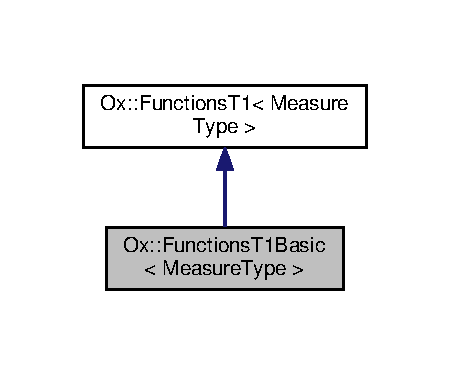
\includegraphics[width=216pt]{class_ox_1_1_functions_t1_basic__inherit__graph}
\end{center}
\end{figure}


Collaboration diagram for Ox\-:\-:Functions\-T1\-Basic$<$ Measure\-Type $>$\-:
\nopagebreak
\begin{figure}[H]
\begin{center}
\leavevmode
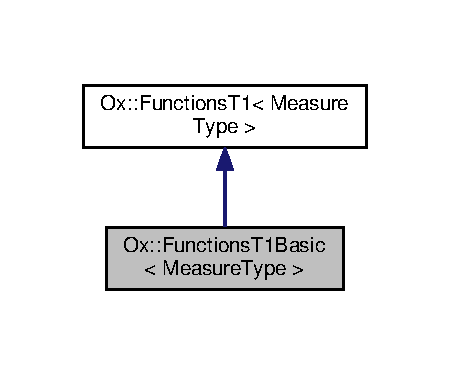
\includegraphics[width=216pt]{class_ox_1_1_functions_t1_basic__coll__graph}
\end{center}
\end{figure}
\subsection*{Public Member Functions}
\begin{DoxyCompactItemize}
\item 
virtual Measure\-Type \hyperlink{class_ox_1_1_functions_t1_basic_ad23b00edd74fdf78c7d21fa82bb66e6e}{calc\-Model\-Value} (Measure\-Type time)
\item 
virtual void \hyperlink{class_ox_1_1_functions_t1_basic_ac9f77d95d7b39f2333b520d3a2e639e9}{calc\-L\-S\-Residuals} (Measure\-Type $\ast$residuals)
\item 
virtual void \hyperlink{class_ox_1_1_functions_t1_basic_a3beaaac6e2e1be4f9bd2e7cba7c51057}{calc\-L\-S\-Jacobian} (Measure\-Type $\ast$jacobian)
\item 
virtual Measure\-Type \hyperlink{class_ox_1_1_functions_t1_basic_adee7b03ad49d28e5dc08a80b2c948da1}{calc\-Cost\-Value} ()
\item 
virtual void \hyperlink{class_ox_1_1_functions_t1_basic_aa6a067295d09882f70eeb34b260c37b7}{calc\-Cost\-Derivative} (Measure\-Type $\ast$derivative)
\item 
\hypertarget{class_ox_1_1_functions_t1_basic_ae3f94c1426a8e6f569b8c70f86122c0b}{virtual \hyperlink{class_ox_1_1_functions_t1_basic_ae3f94c1426a8e6f569b8c70f86122c0b}{$\sim$\-Functions\-T1\-Basic} ()}\label{class_ox_1_1_functions_t1_basic_ae3f94c1426a8e6f569b8c70f86122c0b}

\begin{DoxyCompactList}\small\item\em do not forget about the virtual destructor, see \href{https://stackoverflow.com/questions/461203/when-to-use-virtual-destructors}{\tt https\-://stackoverflow.\-com/questions/461203/when-\/to-\/use-\/virtual-\/destructors} \end{DoxyCompactList}\end{DoxyCompactItemize}
\subsection*{Additional Inherited Members}


\subsection{Detailed Description}
\subsubsection*{template$<$typename Measure\-Type$>$class Ox\-::\-Functions\-T1\-Basic$<$ Measure\-Type $>$}

Container for a basic model function $ A-B\exp(t/T_1^*) $, cost function and Least-\/\-Squares function and derivatives. 


\begin{DoxyTemplParams}{Template Parameters}
{\em Measure\-Type} & \\
\hline
\end{DoxyTemplParams}


\subsection{Member Function Documentation}
\hypertarget{class_ox_1_1_functions_t1_basic_aa6a067295d09882f70eeb34b260c37b7}{\index{Ox\-::\-Functions\-T1\-Basic@{Ox\-::\-Functions\-T1\-Basic}!calc\-Cost\-Derivative@{calc\-Cost\-Derivative}}
\index{calc\-Cost\-Derivative@{calc\-Cost\-Derivative}!Ox::FunctionsT1Basic@{Ox\-::\-Functions\-T1\-Basic}}
\subsubsection[{calc\-Cost\-Derivative}]{\setlength{\rightskip}{0pt plus 5cm}template$<$typename Measure\-Type $>$ void {\bf Ox\-::\-Functions\-T1\-Basic}$<$ Measure\-Type $>$\-::calc\-Cost\-Derivative (
\begin{DoxyParamCaption}
\item[{Measure\-Type $\ast$}]{derivative}
\end{DoxyParamCaption}
)\hspace{0.3cm}{\ttfamily [virtual]}}}\label{class_ox_1_1_functions_t1_basic_aa6a067295d09882f70eeb34b260c37b7}
calc\-Cost\-Derivative the most important function of this class 
\begin{DoxyParams}{Parameters}
{\em derivative} & \\
\hline
\end{DoxyParams}


Implements \hyperlink{class_ox_1_1_functions_t1_a413b0afca183b88613070ae87121ca66}{Ox\-::\-Functions\-T1$<$ Measure\-Type $>$}.

\hypertarget{class_ox_1_1_functions_t1_basic_adee7b03ad49d28e5dc08a80b2c948da1}{\index{Ox\-::\-Functions\-T1\-Basic@{Ox\-::\-Functions\-T1\-Basic}!calc\-Cost\-Value@{calc\-Cost\-Value}}
\index{calc\-Cost\-Value@{calc\-Cost\-Value}!Ox::FunctionsT1Basic@{Ox\-::\-Functions\-T1\-Basic}}
\subsubsection[{calc\-Cost\-Value}]{\setlength{\rightskip}{0pt plus 5cm}template$<$typename Measure\-Type $>$ Measure\-Type {\bf Ox\-::\-Functions\-T1\-Basic}$<$ Measure\-Type $>$\-::calc\-Cost\-Value (
\begin{DoxyParamCaption}
{}
\end{DoxyParamCaption}
)\hspace{0.3cm}{\ttfamily [virtual]}}}\label{class_ox_1_1_functions_t1_basic_adee7b03ad49d28e5dc08a80b2c948da1}
calc\-Cost\-Value the most important function of this class \begin{DoxyReturn}{Returns}

\end{DoxyReturn}


Implements \hyperlink{class_ox_1_1_functions_t1_af1475834e89c9304a96c776f3d5aacbf}{Ox\-::\-Functions\-T1$<$ Measure\-Type $>$}.

\hypertarget{class_ox_1_1_functions_t1_basic_a3beaaac6e2e1be4f9bd2e7cba7c51057}{\index{Ox\-::\-Functions\-T1\-Basic@{Ox\-::\-Functions\-T1\-Basic}!calc\-L\-S\-Jacobian@{calc\-L\-S\-Jacobian}}
\index{calc\-L\-S\-Jacobian@{calc\-L\-S\-Jacobian}!Ox::FunctionsT1Basic@{Ox\-::\-Functions\-T1\-Basic}}
\subsubsection[{calc\-L\-S\-Jacobian}]{\setlength{\rightskip}{0pt plus 5cm}template$<$typename Measure\-Type $>$ void {\bf Ox\-::\-Functions\-T1\-Basic}$<$ Measure\-Type $>$\-::calc\-L\-S\-Jacobian (
\begin{DoxyParamCaption}
\item[{Measure\-Type $\ast$}]{jacobian}
\end{DoxyParamCaption}
)\hspace{0.3cm}{\ttfamily [virtual]}}}\label{class_ox_1_1_functions_t1_basic_a3beaaac6e2e1be4f9bd2e7cba7c51057}
calc\-L\-S\-Jacobian the most important function of this class 
\begin{DoxyParams}{Parameters}
{\em jacobian} & -\/ 2d matrix stored as 1d array \\
\hline
\end{DoxyParams}


Implements \hyperlink{class_ox_1_1_functions_t1_a84e268911eb64919129c8a0cea39344d}{Ox\-::\-Functions\-T1$<$ Measure\-Type $>$}.

\hypertarget{class_ox_1_1_functions_t1_basic_ac9f77d95d7b39f2333b520d3a2e639e9}{\index{Ox\-::\-Functions\-T1\-Basic@{Ox\-::\-Functions\-T1\-Basic}!calc\-L\-S\-Residuals@{calc\-L\-S\-Residuals}}
\index{calc\-L\-S\-Residuals@{calc\-L\-S\-Residuals}!Ox::FunctionsT1Basic@{Ox\-::\-Functions\-T1\-Basic}}
\subsubsection[{calc\-L\-S\-Residuals}]{\setlength{\rightskip}{0pt plus 5cm}template$<$typename Measure\-Type $>$ void {\bf Ox\-::\-Functions\-T1\-Basic}$<$ Measure\-Type $>$\-::calc\-L\-S\-Residuals (
\begin{DoxyParamCaption}
\item[{Measure\-Type $\ast$}]{residuals}
\end{DoxyParamCaption}
)\hspace{0.3cm}{\ttfamily [virtual]}}}\label{class_ox_1_1_functions_t1_basic_ac9f77d95d7b39f2333b520d3a2e639e9}
calc\-L\-S\-Residuals the most important function of this class 
\begin{DoxyParams}{Parameters}
{\em residuals} & \\
\hline
\end{DoxyParams}


Implements \hyperlink{class_ox_1_1_functions_t1_a6c69a4159a92c4ddb71ecba97fcdf6de}{Ox\-::\-Functions\-T1$<$ Measure\-Type $>$}.

\hypertarget{class_ox_1_1_functions_t1_basic_ad23b00edd74fdf78c7d21fa82bb66e6e}{\index{Ox\-::\-Functions\-T1\-Basic@{Ox\-::\-Functions\-T1\-Basic}!calc\-Model\-Value@{calc\-Model\-Value}}
\index{calc\-Model\-Value@{calc\-Model\-Value}!Ox::FunctionsT1Basic@{Ox\-::\-Functions\-T1\-Basic}}
\subsubsection[{calc\-Model\-Value}]{\setlength{\rightskip}{0pt plus 5cm}template$<$typename Measure\-Type $>$ Measure\-Type {\bf Ox\-::\-Functions\-T1\-Basic}$<$ Measure\-Type $>$\-::calc\-Model\-Value (
\begin{DoxyParamCaption}
\item[{Measure\-Type}]{time}
\end{DoxyParamCaption}
)\hspace{0.3cm}{\ttfamily [virtual]}}}\label{class_ox_1_1_functions_t1_basic_ad23b00edd74fdf78c7d21fa82bb66e6e}
calc\-Model\-Value the most important function of this class 
\begin{DoxyParams}{Parameters}
{\em time} & \\
\hline
\end{DoxyParams}
\begin{DoxyReturn}{Returns}
model(time) 
\end{DoxyReturn}


Implements \hyperlink{class_ox_1_1_functions_t1_a2d5f4c9296daf3531e30a562348ad474}{Ox\-::\-Functions\-T1$<$ Measure\-Type $>$}.



The documentation for this class was generated from the following files\-:\begin{DoxyCompactItemize}
\item 
lib/\hyperlink{_ox_functions_t1_basic_8h}{Ox\-Functions\-T1\-Basic.\-h}\item 
lib/\hyperlink{_ox_functions_t1_basic_8hxx}{Ox\-Functions\-T1\-Basic.\-hxx}\end{DoxyCompactItemize}

\hypertarget{class_ox_1_1_image_calculator_t1}{\section{Ox\-:\-:Image\-Calculator\-T1$<$ Measure\-Type $>$ Class Template Reference}
\label{class_ox_1_1_image_calculator_t1}\index{Ox\-::\-Image\-Calculator\-T1$<$ Measure\-Type $>$@{Ox\-::\-Image\-Calculator\-T1$<$ Measure\-Type $>$}}
}
\subsection*{Public Member Functions}
\begin{DoxyCompactItemize}
\item 
\hypertarget{class_ox_1_1_image_calculator_t1_af554bf4191ef1d52469e5bb2fa832a57}{void {\bfseries set\-Use\-Threads} (bool \-\_\-use\-Threads)}\label{class_ox_1_1_image_calculator_t1_af554bf4191ef1d52469e5bb2fa832a57}

\item 
\hypertarget{class_ox_1_1_image_calculator_t1_aea2ffd0ea8668a198c8142a21c1eef4f}{void {\bfseries set\-N\-Cols} (int \-\_\-n\-Cols)}\label{class_ox_1_1_image_calculator_t1_aea2ffd0ea8668a198c8142a21c1eef4f}

\item 
\hypertarget{class_ox_1_1_image_calculator_t1_ab4cbe03b2105cc5e5d61432d3c320ab3}{void {\bfseries set\-N\-Rows} (int \-\_\-n\-Rows)}\label{class_ox_1_1_image_calculator_t1_ab4cbe03b2105cc5e5d61432d3c320ab3}

\item 
\hypertarget{class_ox_1_1_image_calculator_t1_a35729c3ccb7f4e3426a16682cecdb8a1}{void {\bfseries set\-N\-Samples} (int \-\_\-n\-Samples)}\label{class_ox_1_1_image_calculator_t1_a35729c3ccb7f4e3426a16682cecdb8a1}

\item 
\hypertarget{class_ox_1_1_image_calculator_t1_a92cbd8b336a8aaac7c7b9e5b52968454}{void {\bfseries set\-Inv\-Times} (Measure\-Type $\ast$\-\_\-inv\-Times)}\label{class_ox_1_1_image_calculator_t1_a92cbd8b336a8aaac7c7b9e5b52968454}

\item 
\hypertarget{class_ox_1_1_image_calculator_t1_a5193dd7849ec11b2173cb94fb0bcd74b}{void {\bfseries set\-Image\-Mag} (Measure\-Type $\ast$\-\_\-image\-Mag)}\label{class_ox_1_1_image_calculator_t1_a5193dd7849ec11b2173cb94fb0bcd74b}

\item 
\hypertarget{class_ox_1_1_image_calculator_t1_a4506dab7d6ad85807b68ad4b1ab7fb85}{void {\bfseries set\-Image\-Pha} (Measure\-Type $\ast$\-\_\-image\-Pha)}\label{class_ox_1_1_image_calculator_t1_a4506dab7d6ad85807b68ad4b1ab7fb85}

\item 
\hypertarget{class_ox_1_1_image_calculator_t1_a57aa44a0e067f5747dc017be41f15d78}{void {\bfseries set\-Image\-Results} (Measure\-Type $\ast$\-\_\-image\-Results)}\label{class_ox_1_1_image_calculator_t1_a57aa44a0e067f5747dc017be41f15d78}

\item 
\hypertarget{class_ox_1_1_image_calculator_t1_aedd4a349b189cee112c8637757c733c7}{void {\bfseries set\-Calculator\-T1} (\hyperlink{class_ox_1_1_calculator}{Calculator}$<$ Measure\-Type $>$ $\ast$\-\_\-calculator\-T1)}\label{class_ox_1_1_image_calculator_t1_aedd4a349b189cee112c8637757c733c7}

\item 
\hypertarget{class_ox_1_1_image_calculator_t1_ab8670346a47b573558357787b64dc94d}{Measure\-Type $\ast$ {\bfseries get\-Image\-Results} () const }\label{class_ox_1_1_image_calculator_t1_ab8670346a47b573558357787b64dc94d}

\item 
\hypertarget{class_ox_1_1_image_calculator_t1_ad97c2f2b08a7004815445027523f97ed}{virtual int {\bfseries calculate} ()}\label{class_ox_1_1_image_calculator_t1_ad97c2f2b08a7004815445027523f97ed}

\item 
\hypertarget{class_ox_1_1_image_calculator_t1_a3ff9a9627bae210326cfbeebea097cb8}{virtual int {\bfseries calculate\-One\-Thread} (int pos\-Start, int pos\-Stop)}\label{class_ox_1_1_image_calculator_t1_a3ff9a9627bae210326cfbeebea097cb8}

\end{DoxyCompactItemize}
\subsection*{Protected Attributes}
\begin{DoxyCompactItemize}
\item 
\hypertarget{class_ox_1_1_image_calculator_t1_af5f6e72b63b78a87a3723f4f2d71068f}{bool {\bfseries \-\_\-use\-Threads}}\label{class_ox_1_1_image_calculator_t1_af5f6e72b63b78a87a3723f4f2d71068f}

\item 
\hypertarget{class_ox_1_1_image_calculator_t1_a02ee85ff0ffd7cb5b1de9357ab23ce56}{int {\bfseries \-\_\-n\-Cols}}\label{class_ox_1_1_image_calculator_t1_a02ee85ff0ffd7cb5b1de9357ab23ce56}

\item 
\hypertarget{class_ox_1_1_image_calculator_t1_ab3db79a49b848f1a145e6fcbb9c29766}{int {\bfseries \-\_\-n\-Rows}}\label{class_ox_1_1_image_calculator_t1_ab3db79a49b848f1a145e6fcbb9c29766}

\item 
\hypertarget{class_ox_1_1_image_calculator_t1_af5655b9262c2634cc8b4ce0465682b0e}{int {\bfseries \-\_\-n\-Samples}}\label{class_ox_1_1_image_calculator_t1_af5655b9262c2634cc8b4ce0465682b0e}

\item 
\hypertarget{class_ox_1_1_image_calculator_t1_a6bc67b8020a51ecd2defd7ede1954b52}{Measure\-Type $\ast$ {\bfseries \-\_\-inv\-Times}}\label{class_ox_1_1_image_calculator_t1_a6bc67b8020a51ecd2defd7ede1954b52}

\item 
\hypertarget{class_ox_1_1_image_calculator_t1_ab43aaec5a7bae1246c96f366498c2130}{Measure\-Type $\ast$ {\bfseries \-\_\-image\-Mag}}\label{class_ox_1_1_image_calculator_t1_ab43aaec5a7bae1246c96f366498c2130}

\item 
\hypertarget{class_ox_1_1_image_calculator_t1_af804d044be29f0b554c68992d77f22ba}{Measure\-Type $\ast$ {\bfseries \-\_\-image\-Pha}}\label{class_ox_1_1_image_calculator_t1_af804d044be29f0b554c68992d77f22ba}

\item 
\hypertarget{class_ox_1_1_image_calculator_t1_a62bb966f944eae07d9873db02487f850}{Measure\-Type $\ast$ {\bfseries \-\_\-image\-Results}}\label{class_ox_1_1_image_calculator_t1_a62bb966f944eae07d9873db02487f850}

\item 
\hypertarget{class_ox_1_1_image_calculator_t1_a35e200233fd8e1ecdd88c8a74ae4c1d0}{Measure\-Type {\bfseries phase\-Range}}\label{class_ox_1_1_image_calculator_t1_a35e200233fd8e1ecdd88c8a74ae4c1d0}

\item 
\hypertarget{class_ox_1_1_image_calculator_t1_a1ba7f99a15c36c734abe8253cd0de4d5}{\hyperlink{class_ox_1_1_calculator}{Calculator}$<$ Measure\-Type $>$ $\ast$ {\bfseries \-\_\-calculator\-T1}}\label{class_ox_1_1_image_calculator_t1_a1ba7f99a15c36c734abe8253cd0de4d5}

\end{DoxyCompactItemize}


The documentation for this class was generated from the following files\-:\begin{DoxyCompactItemize}
\item 
lib/Ox\-Image\-Calculator\-T1.\-h\item 
lib/Ox\-Image\-Calculator\-T1.\-hxx\end{DoxyCompactItemize}

\hypertarget{class_k_w_util}{\section{K\-W\-Util Class Reference}
\label{class_k_w_util}\index{K\-W\-Util@{K\-W\-Util}}
}
\subsection*{Static Public Member Functions}
\begin{DoxyCompactItemize}
\item 
\hypertarget{class_k_w_util_a5d14be8edc626d6b30b31c8d85c64d00}{{\footnotesize template$<$typename T\-Y\-P\-E $>$ }\\static void {\bfseries print\-K\-W} (bool do\-Print, char $\ast$fmt,...)}\label{class_k_w_util_a5d14be8edc626d6b30b31c8d85c64d00}

\item 
\hypertarget{class_k_w_util_a74cbba48bf115ff4ddb90e4c8abfaaac}{{\footnotesize template$<$typename T\-Y\-P\-E1 , typename T\-Y\-P\-E2 $>$ }\\static void {\bfseries copy\-Array\-To\-Array} (int n\-Samples, T\-Y\-P\-E1 $\ast$array\-To, const T\-Y\-P\-E2 $\ast$array\-From)}\label{class_k_w_util_a74cbba48bf115ff4ddb90e4c8abfaaac}

\item 
{\footnotesize template$<$typename T\-Y\-P\-E $>$ }\\static void \hyperlink{class_k_w_util_acc956bb7cbedc39fbca11a6414b66dac}{print\-Vector} (const std\-::string \&name, const std\-::vector$<$ T\-Y\-P\-E $>$ vector)
\item 
{\footnotesize template$<$typename T\-Y\-P\-E $>$ }\\static void \hyperlink{class_k_w_util_aec00dd2420ac8d850284db70c71c1c16}{print\-Vector\-Newline} (const std\-::string \&name, const std\-::vector$<$ T\-Y\-P\-E $>$ vector)
\item 
\hypertarget{class_k_w_util_a9a809d578ed4b3647b7a92a8ee349a0e}{{\footnotesize template$<$typename T\-Y\-P\-E $>$ }\\static void {\bfseries print\-Array} (int n\-Samples, const T\-Y\-P\-E $\ast$myarray)}\label{class_k_w_util_a9a809d578ed4b3647b7a92a8ee349a0e}

\item 
\hypertarget{class_k_w_util_a43228ea0afd7071af2d990ee550472e0}{{\footnotesize template$<$typename T\-Y\-P\-E $>$ }\\static void {\bfseries print\-Array} (int n\-Samples, const T\-Y\-P\-E $\ast$myarray, int width)}\label{class_k_w_util_a43228ea0afd7071af2d990ee550472e0}

\item 
\hypertarget{class_k_w_util_aa537bb86732154b9ad1317e851afccfd}{{\footnotesize template$<$typename T\-Y\-P\-E $>$ }\\static void {\bfseries print\-Array} (int n\-Samples, const T\-Y\-P\-E $\ast$myarray, char $\ast$text)}\label{class_k_w_util_aa537bb86732154b9ad1317e851afccfd}

\item 
\hypertarget{class_k_w_util_a551666cf04781258441f4d5a77c6a7d8}{{\footnotesize template$<$typename T\-Y\-P\-E $>$ }\\static void {\bfseries print\-Array} (bool do\-Print, int n\-Samples, const T\-Y\-P\-E $\ast$myarray)}\label{class_k_w_util_a551666cf04781258441f4d5a77c6a7d8}

\item 
\hypertarget{class_k_w_util_a5eafacfaa0ea74867d2b37cf22558644}{{\footnotesize template$<$typename T\-Y\-P\-E $>$ }\\static void {\bfseries print\-Array} (bool do\-Print, int n\-Samples, const T\-Y\-P\-E $\ast$myarray, char $\ast$text)}\label{class_k_w_util_a5eafacfaa0ea74867d2b37cf22558644}

\item 
\hypertarget{class_k_w_util_a0d00bcaaee4bf9fe1ea3f28c39db766d}{{\footnotesize template$<$typename T\-Y\-P\-E $>$ }\\static void {\bfseries print\-Array2\-D} (int n\-Rows, int n\-Cols, T\-Y\-P\-E $\ast$$\ast$myarray)}\label{class_k_w_util_a0d00bcaaee4bf9fe1ea3f28c39db766d}

\item 
\hypertarget{class_k_w_util_a8ca8f9d0826b637aee5285af196431a0}{{\footnotesize template$<$typename T\-Y\-P\-E $>$ }\\static void {\bfseries print\-Array2\-D} (int n\-Rows, int n\-Cols, T\-Y\-P\-E $\ast$$\ast$myarray, char $\ast$text)}\label{class_k_w_util_a8ca8f9d0826b637aee5285af196431a0}

\item 
\hypertarget{class_k_w_util_a2907060d81976090c40829107159666d}{{\footnotesize template$<$typename T\-Y\-P\-E $>$ }\\static void {\bfseries print\-Array2\-D} (bool do\-Print, int n\-Rows, int n\-Cols, T\-Y\-P\-E $\ast$$\ast$myarray)}\label{class_k_w_util_a2907060d81976090c40829107159666d}

\item 
\hypertarget{class_k_w_util_a59aabe5a32605da8367ca84c3ad3a0ab}{{\footnotesize template$<$typename T\-Y\-P\-E $>$ }\\static void {\bfseries print\-Array2\-D} (bool do\-Print, int n\-Rows, int n\-Cols, T\-Y\-P\-E $\ast$$\ast$myarray, char $\ast$text)}\label{class_k_w_util_a59aabe5a32605da8367ca84c3ad3a0ab}

\item 
\hypertarget{class_k_w_util_aaffd937290f71df67551a6f2a00e1660}{{\footnotesize template$<$typename T\-Y\-P\-E $>$ }\\static void {\bfseries print\-Std\-Vector} (const std\-::vector$<$ T\-Y\-P\-E $>$ myvector)}\label{class_k_w_util_aaffd937290f71df67551a6f2a00e1660}

\item 
\hypertarget{class_k_w_util_a8d69c11c8b97c2bc5aee5449ece9b11d}{{\footnotesize template$<$typename T\-Y\-P\-E $>$ }\\static void {\bfseries print\-Std\-Vector} (const std\-::vector$<$ T\-Y\-P\-E $>$ myvector, char $\ast$text)}\label{class_k_w_util_a8d69c11c8b97c2bc5aee5449ece9b11d}

\item 
\hypertarget{class_k_w_util_a684d6abf0326e8d495f709c2b1d82ea2}{{\footnotesize template$<$typename T\-Y\-P\-E $>$ }\\static void {\bfseries print\-Std\-Vector} (bool do\-Print, const std\-::vector$<$ T\-Y\-P\-E $>$ myvector)}\label{class_k_w_util_a684d6abf0326e8d495f709c2b1d82ea2}

\item 
\hypertarget{class_k_w_util_ac17252f672282e2f60e76d594ed2d8f7}{{\footnotesize template$<$typename T\-Y\-P\-E $>$ }\\static void {\bfseries print\-Std\-Vector} (bool do\-Print, const std\-::vector$<$ T\-Y\-P\-E $>$ myvector, char $\ast$text)}\label{class_k_w_util_ac17252f672282e2f60e76d594ed2d8f7}

\item 
\hypertarget{class_k_w_util_a6ed5d213169247c4b3fe3ed2fb96dd88}{{\footnotesize template$<$typename T\-Y\-P\-E $>$ }\\static void {\bfseries swap} (T\-Y\-P\-E \&a, T\-Y\-P\-E \&b)}\label{class_k_w_util_a6ed5d213169247c4b3fe3ed2fb96dd88}

\item 
\hypertarget{class_k_w_util_a707d699ad01c87ba21e06fe28de85712}{{\footnotesize template$<$typename T\-Y\-P\-E $>$ }\\static T\-Y\-P\-E {\bfseries max} (T\-Y\-P\-E a, T\-Y\-P\-E b)}\label{class_k_w_util_a707d699ad01c87ba21e06fe28de85712}

\item 
\hypertarget{class_k_w_util_af1b3640361810ba75435a850d73a2413}{{\footnotesize template$<$typename T\-Y\-P\-E $>$ }\\static T\-Y\-P\-E {\bfseries min} (T\-Y\-P\-E a, T\-Y\-P\-E b)}\label{class_k_w_util_af1b3640361810ba75435a850d73a2413}

\item 
\hypertarget{class_k_w_util_abe27306f912197863466e7c68d3c66fb}{{\footnotesize template$<$typename T\-Y\-P\-E $>$ }\\static T\-Y\-P\-E {\bfseries calc\-Sum\-Array} (int n\-Samples, const T\-Y\-P\-E $\ast$myarray)}\label{class_k_w_util_abe27306f912197863466e7c68d3c66fb}

\item 
\hypertarget{class_k_w_util_ad9cb19db7d541d5ca5a60c6a28b922e1}{{\footnotesize template$<$typename T\-Y\-P\-E $>$ }\\static double {\bfseries calc\-Mean\-Array} (int n\-Samples, const T\-Y\-P\-E $\ast$myarray)}\label{class_k_w_util_ad9cb19db7d541d5ca5a60c6a28b922e1}

\item 
\hypertarget{class_k_w_util_a6c10285ae2d87ccda6ddaa18c81dea39}{{\footnotesize template$<$typename T\-Y\-P\-E $>$ }\\static double {\bfseries calc\-Median\-Array} (int n\-Samples, const T\-Y\-P\-E $\ast$myarray)}\label{class_k_w_util_a6c10285ae2d87ccda6ddaa18c81dea39}

\item 
\hypertarget{class_k_w_util_ad9d38c641f6b227be4418acf404170d4}{{\footnotesize template$<$typename T\-Y\-P\-E $>$ }\\static double {\bfseries calc\-Standard\-Deviation\-Array} (int n\-Samples, const T\-Y\-P\-E $\ast$myarray)}\label{class_k_w_util_ad9d38c641f6b227be4418acf404170d4}

\item 
\hypertarget{class_k_w_util_ae26dd38b1c5c823fa37129520bb4cc47}{{\footnotesize template$<$typename T\-Y\-P\-E $>$ }\\static double {\bfseries calc\-R2ss} (int n\-Samples, const T\-Y\-P\-E $\ast$fitted, const T\-Y\-P\-E $\ast$ysignal)}\label{class_k_w_util_ae26dd38b1c5c823fa37129520bb4cc47}

\item 
\hypertarget{class_k_w_util_a9eecfdafa3ae5e493830181fa7ea8fa3}{{\footnotesize template$<$typename T\-Y\-P\-E $>$ }\\static double {\bfseries calc\-R2cor} (int n\-Samples, const T\-Y\-P\-E $\ast$fitted, const T\-Y\-P\-E $\ast$ysignal)}\label{class_k_w_util_a9eecfdafa3ae5e493830181fa7ea8fa3}

\item 
\hypertarget{class_k_w_util_ac7633e5346a8b4ad6b2d1d960eb22fc9}{{\footnotesize template$<$typename T\-Y\-P\-E $>$ }\\static double {\bfseries S\-K\-P\-Lin\-Reg} (const T\-Y\-P\-E $\ast$datax, const T\-Y\-P\-E $\ast$datay, int n\-Samples, T\-Y\-P\-E \&rslope, T\-Y\-P\-E \&roffset)}\label{class_k_w_util_ac7633e5346a8b4ad6b2d1d960eb22fc9}

\item 
\hypertarget{class_k_w_util_adea3028ddaac44e13ab60460b0e50452}{{\footnotesize template$<$typename T\-Y\-P\-E $>$ }\\static void {\bfseries S\-K\-Psort} (int n\-Samples, const T\-Y\-P\-E $\ast$myarray, int $\ast$index)}\label{class_k_w_util_adea3028ddaac44e13ab60460b0e50452}

\item 
\hypertarget{class_k_w_util_aacc2b444dd10145dea4367714527efa9}{{\footnotesize template$<$typename T\-Y\-P\-E $>$ }\\static void {\bfseries quick\-Sort} (int n\-Samples, T\-Y\-P\-E $\ast$myarray)}\label{class_k_w_util_aacc2b444dd10145dea4367714527efa9}

\item 
\hypertarget{class_k_w_util_aba1906d9b0de1262e0ce837b15e8401f}{{\footnotesize template$<$typename T\-Y\-P\-E $>$ }\\static void {\bfseries quick\-Sort\-Index} (int n\-Samples, T\-Y\-P\-E $\ast$myarray, int $\ast$index\-Array)}\label{class_k_w_util_aba1906d9b0de1262e0ce837b15e8401f}

\item 
\hypertarget{class_k_w_util_a2e55b0bcf1bbf1155654b748a7064cbf}{{\footnotesize template$<$typename T\-Y\-P\-E $>$ }\\static T\-Y\-P\-E {\bfseries get\-Chi\-Sqrt} (T\-Y\-P\-E last\-F\-Value, int n\-Samples)}\label{class_k_w_util_a2e55b0bcf1bbf1155654b748a7064cbf}

\item 
{\footnotesize template$<$typename T\-Y\-P\-E $>$ }\\static int \hyperlink{class_k_w_util_a80504801c382f1ac367bcf0787fb18c2}{calc\-Matrix\-Inverse3x3} (const T\-Y\-P\-E $\ast$matrix, T\-Y\-P\-E $\ast$matrix\-Inverse)
\item 
\hypertarget{class_k_w_util_a6401111c5ce49eb97e1c79bae84b3868}{{\footnotesize template$<$typename T\-Y\-P\-E $>$ }\\static T\-Y\-P\-E {\bfseries M\-O\-L\-L\-I\-\_\-min} (T\-Y\-P\-E a\mbox{[}$\,$\mbox{]}, int n, int $\ast$indm)}\label{class_k_w_util_a6401111c5ce49eb97e1c79bae84b3868}

\item 
\hypertarget{class_k_w_util_af0fee5e9d89e7c029c346804480d5832}{{\footnotesize template$<$typename T\-Y\-P\-E $>$ }\\static T\-Y\-P\-E {\bfseries M\-O\-L\-L\-I\-\_\-max} (T\-Y\-P\-E a\mbox{[}$\,$\mbox{]}, int n, int $\ast$indm)}\label{class_k_w_util_af0fee5e9d89e7c029c346804480d5832}

\item 
\hypertarget{class_k_w_util_a10aaa83c83c801ef07c95a29e1acdc4e}{{\footnotesize template$<$typename T\-Y\-P\-E $>$ }\\static std\-::string {\bfseries Number\-To\-String} (T\-Y\-P\-E Number)}\label{class_k_w_util_a10aaa83c83c801ef07c95a29e1acdc4e}

\item 
\hypertarget{class_k_w_util_adea4c36750f518d1f2c90af14742a0f6}{{\footnotesize template$<$typename T\-Y\-P\-E $>$ }\\static T\-Y\-P\-E {\bfseries String\-To\-Number} (const std\-::string \&Text)}\label{class_k_w_util_adea4c36750f518d1f2c90af14742a0f6}

\item 
\hypertarget{class_k_w_util_a21813a6377e55fa15c70f64afb2feb51}{{\footnotesize template$<$typename T\-Y\-P\-E $>$ }\\static T\-Y\-P\-E {\bfseries dicom\-Time2\-Seconds} (std\-::string dicom\-Time\-String)}\label{class_k_w_util_a21813a6377e55fa15c70f64afb2feb51}

\item 
\hypertarget{class_k_w_util_a498350d10204849240a945ea682ecc98}{{\footnotesize template$<$typename T\-Y\-P\-E $>$ }\\static std\-::vector$<$ int $>$ {\bfseries bounds} (int parts, int mem)}\label{class_k_w_util_a498350d10204849240a945ea682ecc98}

\item 
\hypertarget{class_k_w_util_a19d7a4b4320a3b9d8ff06e4d296e2893}{static std\-::string {\bfseries Path\-Separator} ()}\label{class_k_w_util_a19d7a4b4320a3b9d8ff06e4d296e2893}

\item 
\hypertarget{class_k_w_util_afe6ad66b5fe06a8b42918634076ab056}{static void {\bfseries split\-Filename} (const std\-::string \&str, std\-::string \&path, std\-::string \&file)}\label{class_k_w_util_afe6ad66b5fe06a8b42918634076ab056}

\item 
\hypertarget{class_k_w_util_a70a639cebc8982645a9ba44f73b93d85}{static std\-::vector$<$ std\-::string $>$ {\bfseries read\-File} (const std\-::string file\-Path)}\label{class_k_w_util_a70a639cebc8982645a9ba44f73b93d85}

\end{DoxyCompactItemize}


\subsection{Member Function Documentation}
\hypertarget{class_k_w_util_a80504801c382f1ac367bcf0787fb18c2}{\index{K\-W\-Util@{K\-W\-Util}!calc\-Matrix\-Inverse3x3@{calc\-Matrix\-Inverse3x3}}
\index{calc\-Matrix\-Inverse3x3@{calc\-Matrix\-Inverse3x3}!KWUtil@{K\-W\-Util}}
\subsubsection[{calc\-Matrix\-Inverse3x3}]{\setlength{\rightskip}{0pt plus 5cm}template$<$typename T\-Y\-P\-E $>$ int K\-W\-Util\-::calc\-Matrix\-Inverse3x3 (
\begin{DoxyParamCaption}
\item[{const T\-Y\-P\-E $\ast$}]{matrix, }
\item[{T\-Y\-P\-E $\ast$}]{matrix\-Inverse}
\end{DoxyParamCaption}
)\hspace{0.3cm}{\ttfamily [static]}}}\label{class_k_w_util_a80504801c382f1ac367bcf0787fb18c2}

\begin{DoxyTemplParams}{Template Parameters}
{\em T\-Y\-P\-E} & \\
\hline
\end{DoxyTemplParams}

\begin{DoxyParams}{Parameters}
{\em matrix} & -\/ pointer to array with indices \mbox{[}0 1 2; 3 4 5; 6 7 8\mbox{]} \\
\hline
{\em matrix\-Inverse} & -\/ pointer to with indices \mbox{[}0 1 2; 3 4 5; 6 7 8\mbox{]}. Fills the inverse matix if determinant != 0 or zero matrix if det == 0 \\
\hline
\end{DoxyParams}
\begin{DoxyReturn}{Returns}
0 if success, 1 if det == 0 
\end{DoxyReturn}
\hypertarget{class_k_w_util_acc956bb7cbedc39fbca11a6414b66dac}{\index{K\-W\-Util@{K\-W\-Util}!print\-Vector@{print\-Vector}}
\index{print\-Vector@{print\-Vector}!KWUtil@{K\-W\-Util}}
\subsubsection[{print\-Vector}]{\setlength{\rightskip}{0pt plus 5cm}template$<$typename T\-Y\-P\-E $>$ void K\-W\-Util\-::print\-Vector (
\begin{DoxyParamCaption}
\item[{const std\-::string \&}]{name, }
\item[{const std\-::vector$<$ T\-Y\-P\-E $>$}]{vector}
\end{DoxyParamCaption}
)\hspace{0.3cm}{\ttfamily [static]}}}\label{class_k_w_util_acc956bb7cbedc39fbca11a6414b66dac}
print\-Vector 
\begin{DoxyTemplParams}{Template Parameters}
{\em T\-Y\-P\-E} & \\
\hline
\end{DoxyTemplParams}

\begin{DoxyParams}{Parameters}
{\em name} & \\
\hline
{\em vector} & \\
\hline
\end{DoxyParams}
\hypertarget{class_k_w_util_aec00dd2420ac8d850284db70c71c1c16}{\index{K\-W\-Util@{K\-W\-Util}!print\-Vector\-Newline@{print\-Vector\-Newline}}
\index{print\-Vector\-Newline@{print\-Vector\-Newline}!KWUtil@{K\-W\-Util}}
\subsubsection[{print\-Vector\-Newline}]{\setlength{\rightskip}{0pt plus 5cm}template$<$typename T\-Y\-P\-E $>$ void K\-W\-Util\-::print\-Vector\-Newline (
\begin{DoxyParamCaption}
\item[{const std\-::string \&}]{name, }
\item[{const std\-::vector$<$ T\-Y\-P\-E $>$}]{vector}
\end{DoxyParamCaption}
)\hspace{0.3cm}{\ttfamily [static]}}}\label{class_k_w_util_aec00dd2420ac8d850284db70c71c1c16}
print\-Vectorn with newlines after every element 
\begin{DoxyTemplParams}{Template Parameters}
{\em T\-Y\-P\-E} & \\
\hline
\end{DoxyTemplParams}

\begin{DoxyParams}{Parameters}
{\em name} & \\
\hline
{\em vector} & \\
\hline
\end{DoxyParams}


The documentation for this class was generated from the following files\-:\begin{DoxyCompactItemize}
\item 
lib/K\-W\-Util.\-h\item 
lib/K\-W\-Util.\-hxx\end{DoxyCompactItemize}

\hypertarget{classitk_1_1_n_shmolli_samples_used_to123_image_filter}{\section{itk\-:\-:N\-Shmolli\-Samples\-Used\-To123\-Image\-Filter$<$ T\-Image $>$ Class Template Reference}
\label{classitk_1_1_n_shmolli_samples_used_to123_image_filter}\index{itk\-::\-N\-Shmolli\-Samples\-Used\-To123\-Image\-Filter$<$ T\-Image $>$@{itk\-::\-N\-Shmolli\-Samples\-Used\-To123\-Image\-Filter$<$ T\-Image $>$}}
}


Inheritance diagram for itk\-:\-:N\-Shmolli\-Samples\-Used\-To123\-Image\-Filter$<$ T\-Image $>$\-:
\nopagebreak
\begin{figure}[H]
\begin{center}
\leavevmode
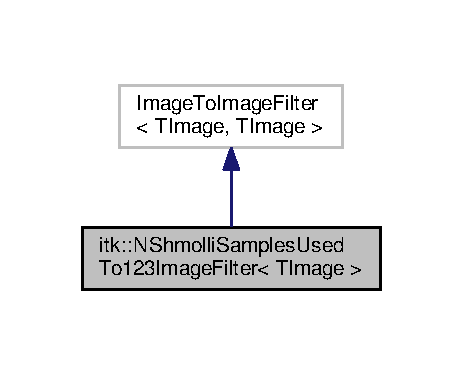
\includegraphics[width=222pt]{classitk_1_1_n_shmolli_samples_used_to123_image_filter__inherit__graph}
\end{center}
\end{figure}


Collaboration diagram for itk\-:\-:N\-Shmolli\-Samples\-Used\-To123\-Image\-Filter$<$ T\-Image $>$\-:
\nopagebreak
\begin{figure}[H]
\begin{center}
\leavevmode
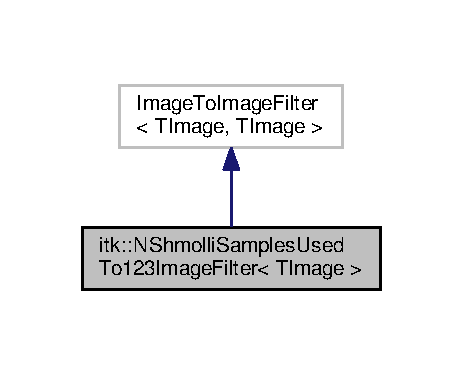
\includegraphics[width=222pt]{classitk_1_1_n_shmolli_samples_used_to123_image_filter__coll__graph}
\end{center}
\end{figure}
\subsection*{Public Types}
\begin{DoxyCompactItemize}
\item 
typedef \\*
\hyperlink{classitk_1_1_n_shmolli_samples_used_to123_image_filter}{N\-Shmolli\-Samples\-Used\-To123\-Image\-Filter} \hyperlink{classitk_1_1_n_shmolli_samples_used_to123_image_filter_aa227171fdb715a86680dae7b2aeb60ca}{Self}
\item 
\hypertarget{classitk_1_1_n_shmolli_samples_used_to123_image_filter_a6eb48e2e880a9eaa080bcd6c97f1b62f}{typedef Image\-To\-Image\-Filter\\*
$<$ T\-Image, T\-Image $>$ {\bfseries Superclass}}\label{classitk_1_1_n_shmolli_samples_used_to123_image_filter_a6eb48e2e880a9eaa080bcd6c97f1b62f}

\item 
\hypertarget{classitk_1_1_n_shmolli_samples_used_to123_image_filter_a1b3d0c2271ece8ef8dec873c6ebaec3b}{typedef Smart\-Pointer$<$ \hyperlink{classitk_1_1_n_shmolli_samples_used_to123_image_filter_aa227171fdb715a86680dae7b2aeb60ca}{Self} $>$ {\bfseries Pointer}}\label{classitk_1_1_n_shmolli_samples_used_to123_image_filter_a1b3d0c2271ece8ef8dec873c6ebaec3b}

\item 
\hypertarget{classitk_1_1_n_shmolli_samples_used_to123_image_filter_acc79dbf838828af74a893d267d18e3f3}{typedef T\-Image\-::\-Pixel\-Type {\bfseries Pixel\-Type\-In}}\label{classitk_1_1_n_shmolli_samples_used_to123_image_filter_acc79dbf838828af74a893d267d18e3f3}

\item 
\hypertarget{classitk_1_1_n_shmolli_samples_used_to123_image_filter_ad1008cfca5a90336b303c2fa1c7ae2ec}{typedef T\-Image\-::\-Pixel\-Type {\bfseries Pixel\-Type\-Out}}\label{classitk_1_1_n_shmolli_samples_used_to123_image_filter_ad1008cfca5a90336b303c2fa1c7ae2ec}

\end{DoxyCompactItemize}
\subsection*{Public Member Functions}
\begin{DoxyCompactItemize}
\item 
\hyperlink{classitk_1_1_n_shmolli_samples_used_to123_image_filter_a0fdd8bb40334c5a00bed7e53b3ce41b9}{itk\-New\-Macro} (\hyperlink{classitk_1_1_n_shmolli_samples_used_to123_image_filter_aa227171fdb715a86680dae7b2aeb60ca}{Self})
\item 
\hyperlink{classitk_1_1_n_shmolli_samples_used_to123_image_filter_a88bd0d5af2509a14869d466a70bdbb25}{itk\-Type\-Macro} (Ox\-Colorbar\-Image\-Filter, Image\-To\-Image\-Filter)
\end{DoxyCompactItemize}
\subsection*{Protected Member Functions}
\begin{DoxyCompactItemize}
\item 
\hyperlink{classitk_1_1_n_shmolli_samples_used_to123_image_filter_a7ab0731450a68f872c8e2888cf4eee5e}{N\-Shmolli\-Samples\-Used\-To123\-Image\-Filter} ()
\item 
\hyperlink{classitk_1_1_n_shmolli_samples_used_to123_image_filter_ab65e63793d21e7f775dc85eea9a6c168}{$\sim$\-N\-Shmolli\-Samples\-Used\-To123\-Image\-Filter} ()
\item 
virtual void \hyperlink{classitk_1_1_n_shmolli_samples_used_to123_image_filter_a1cd4d595fe98ea551673e4f7a2a8ca9f}{Generate\-Data} () I\-T\-K\-\_\-\-O\-V\-E\-R\-R\-I\-D\-E
\end{DoxyCompactItemize}


\subsection{Member Typedef Documentation}
\hypertarget{classitk_1_1_n_shmolli_samples_used_to123_image_filter_aa227171fdb715a86680dae7b2aeb60ca}{\index{itk\-::\-N\-Shmolli\-Samples\-Used\-To123\-Image\-Filter@{itk\-::\-N\-Shmolli\-Samples\-Used\-To123\-Image\-Filter}!Self@{Self}}
\index{Self@{Self}!itk::NShmolliSamplesUsedTo123ImageFilter@{itk\-::\-N\-Shmolli\-Samples\-Used\-To123\-Image\-Filter}}
\subsubsection[{Self}]{\setlength{\rightskip}{0pt plus 5cm}template$<$typename T\-Image $>$ typedef {\bf N\-Shmolli\-Samples\-Used\-To123\-Image\-Filter} {\bf itk\-::\-N\-Shmolli\-Samples\-Used\-To123\-Image\-Filter}$<$ T\-Image $>$\-::{\bf Self}}}\label{classitk_1_1_n_shmolli_samples_used_to123_image_filter_aa227171fdb715a86680dae7b2aeb60ca}
Standard class typedefs. 

\subsection{Constructor \& Destructor Documentation}
\hypertarget{classitk_1_1_n_shmolli_samples_used_to123_image_filter_a7ab0731450a68f872c8e2888cf4eee5e}{\index{itk\-::\-N\-Shmolli\-Samples\-Used\-To123\-Image\-Filter@{itk\-::\-N\-Shmolli\-Samples\-Used\-To123\-Image\-Filter}!N\-Shmolli\-Samples\-Used\-To123\-Image\-Filter@{N\-Shmolli\-Samples\-Used\-To123\-Image\-Filter}}
\index{N\-Shmolli\-Samples\-Used\-To123\-Image\-Filter@{N\-Shmolli\-Samples\-Used\-To123\-Image\-Filter}!itk::NShmolliSamplesUsedTo123ImageFilter@{itk\-::\-N\-Shmolli\-Samples\-Used\-To123\-Image\-Filter}}
\subsubsection[{N\-Shmolli\-Samples\-Used\-To123\-Image\-Filter}]{\setlength{\rightskip}{0pt plus 5cm}template$<$typename T\-Image $>$ {\bf itk\-::\-N\-Shmolli\-Samples\-Used\-To123\-Image\-Filter}$<$ T\-Image $>$\-::{\bf N\-Shmolli\-Samples\-Used\-To123\-Image\-Filter} (
\begin{DoxyParamCaption}
{}
\end{DoxyParamCaption}
)\hspace{0.3cm}{\ttfamily [inline]}, {\ttfamily [protected]}}}\label{classitk_1_1_n_shmolli_samples_used_to123_image_filter_a7ab0731450a68f872c8e2888cf4eee5e}
Constructor. \hypertarget{classitk_1_1_n_shmolli_samples_used_to123_image_filter_ab65e63793d21e7f775dc85eea9a6c168}{\index{itk\-::\-N\-Shmolli\-Samples\-Used\-To123\-Image\-Filter@{itk\-::\-N\-Shmolli\-Samples\-Used\-To123\-Image\-Filter}!$\sim$\-N\-Shmolli\-Samples\-Used\-To123\-Image\-Filter@{$\sim$\-N\-Shmolli\-Samples\-Used\-To123\-Image\-Filter}}
\index{$\sim$\-N\-Shmolli\-Samples\-Used\-To123\-Image\-Filter@{$\sim$\-N\-Shmolli\-Samples\-Used\-To123\-Image\-Filter}!itk::NShmolliSamplesUsedTo123ImageFilter@{itk\-::\-N\-Shmolli\-Samples\-Used\-To123\-Image\-Filter}}
\subsubsection[{$\sim$\-N\-Shmolli\-Samples\-Used\-To123\-Image\-Filter}]{\setlength{\rightskip}{0pt plus 5cm}template$<$typename T\-Image $>$ {\bf itk\-::\-N\-Shmolli\-Samples\-Used\-To123\-Image\-Filter}$<$ T\-Image $>$\-::$\sim${\bf N\-Shmolli\-Samples\-Used\-To123\-Image\-Filter} (
\begin{DoxyParamCaption}
{}
\end{DoxyParamCaption}
)\hspace{0.3cm}{\ttfamily [inline]}, {\ttfamily [protected]}}}\label{classitk_1_1_n_shmolli_samples_used_to123_image_filter_ab65e63793d21e7f775dc85eea9a6c168}
Destructor. 

\subsection{Member Function Documentation}
\hypertarget{classitk_1_1_n_shmolli_samples_used_to123_image_filter_a1cd4d595fe98ea551673e4f7a2a8ca9f}{\index{itk\-::\-N\-Shmolli\-Samples\-Used\-To123\-Image\-Filter@{itk\-::\-N\-Shmolli\-Samples\-Used\-To123\-Image\-Filter}!Generate\-Data@{Generate\-Data}}
\index{Generate\-Data@{Generate\-Data}!itk::NShmolliSamplesUsedTo123ImageFilter@{itk\-::\-N\-Shmolli\-Samples\-Used\-To123\-Image\-Filter}}
\subsubsection[{Generate\-Data}]{\setlength{\rightskip}{0pt plus 5cm}template$<$typename T\-Image $>$ virtual void {\bf itk\-::\-N\-Shmolli\-Samples\-Used\-To123\-Image\-Filter}$<$ T\-Image $>$\-::Generate\-Data (
\begin{DoxyParamCaption}
{}
\end{DoxyParamCaption}
)\hspace{0.3cm}{\ttfamily [protected]}, {\ttfamily [virtual]}}}\label{classitk_1_1_n_shmolli_samples_used_to123_image_filter_a1cd4d595fe98ea551673e4f7a2a8ca9f}
Does the real work. \hypertarget{classitk_1_1_n_shmolli_samples_used_to123_image_filter_a0fdd8bb40334c5a00bed7e53b3ce41b9}{\index{itk\-::\-N\-Shmolli\-Samples\-Used\-To123\-Image\-Filter@{itk\-::\-N\-Shmolli\-Samples\-Used\-To123\-Image\-Filter}!itk\-New\-Macro@{itk\-New\-Macro}}
\index{itk\-New\-Macro@{itk\-New\-Macro}!itk::NShmolliSamplesUsedTo123ImageFilter@{itk\-::\-N\-Shmolli\-Samples\-Used\-To123\-Image\-Filter}}
\subsubsection[{itk\-New\-Macro}]{\setlength{\rightskip}{0pt plus 5cm}template$<$typename T\-Image $>$ {\bf itk\-::\-N\-Shmolli\-Samples\-Used\-To123\-Image\-Filter}$<$ T\-Image $>$\-::itk\-New\-Macro (
\begin{DoxyParamCaption}
\item[{{\bf Self}}]{}
\end{DoxyParamCaption}
)}}\label{classitk_1_1_n_shmolli_samples_used_to123_image_filter_a0fdd8bb40334c5a00bed7e53b3ce41b9}
Method for creation through the object factory. \hypertarget{classitk_1_1_n_shmolli_samples_used_to123_image_filter_a88bd0d5af2509a14869d466a70bdbb25}{\index{itk\-::\-N\-Shmolli\-Samples\-Used\-To123\-Image\-Filter@{itk\-::\-N\-Shmolli\-Samples\-Used\-To123\-Image\-Filter}!itk\-Type\-Macro@{itk\-Type\-Macro}}
\index{itk\-Type\-Macro@{itk\-Type\-Macro}!itk::NShmolliSamplesUsedTo123ImageFilter@{itk\-::\-N\-Shmolli\-Samples\-Used\-To123\-Image\-Filter}}
\subsubsection[{itk\-Type\-Macro}]{\setlength{\rightskip}{0pt plus 5cm}template$<$typename T\-Image $>$ {\bf itk\-::\-N\-Shmolli\-Samples\-Used\-To123\-Image\-Filter}$<$ T\-Image $>$\-::itk\-Type\-Macro (
\begin{DoxyParamCaption}
\item[{Ox\-Colorbar\-Image\-Filter}]{, }
\item[{Image\-To\-Image\-Filter}]{}
\end{DoxyParamCaption}
)}}\label{classitk_1_1_n_shmolli_samples_used_to123_image_filter_a88bd0d5af2509a14869d466a70bdbb25}
Run-\/time type information (and related methods). 

The documentation for this class was generated from the following file\-:\begin{DoxyCompactItemize}
\item 
lib/itk\-N\-Shmolli\-Samples\-Used\-To123\-Image\-Filter.\-h\end{DoxyCompactItemize}

\hypertarget{classitk_1_1_read_file_list_filter}{\section{itk\-:\-:Read\-File\-List\-Filter$<$ T\-Image $>$ Class Template Reference}
\label{classitk_1_1_read_file_list_filter}\index{itk\-::\-Read\-File\-List\-Filter$<$ T\-Image $>$@{itk\-::\-Read\-File\-List\-Filter$<$ T\-Image $>$}}
}


Inheritance diagram for itk\-:\-:Read\-File\-List\-Filter$<$ T\-Image $>$\-:
\nopagebreak
\begin{figure}[H]
\begin{center}
\leavevmode
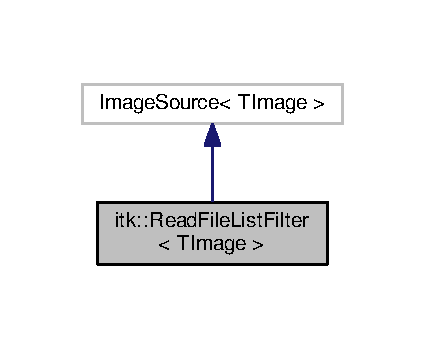
\includegraphics[width=204pt]{classitk_1_1_read_file_list_filter__inherit__graph}
\end{center}
\end{figure}


Collaboration diagram for itk\-:\-:Read\-File\-List\-Filter$<$ T\-Image $>$\-:
\nopagebreak
\begin{figure}[H]
\begin{center}
\leavevmode
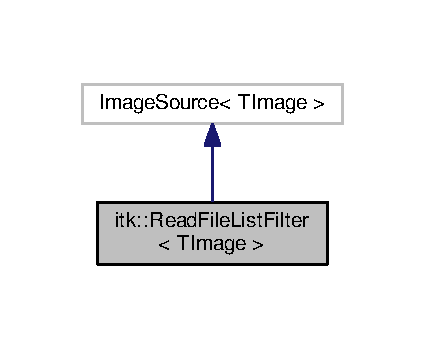
\includegraphics[width=204pt]{classitk_1_1_read_file_list_filter__coll__graph}
\end{center}
\end{figure}
\subsection*{Public Types}
\begin{DoxyCompactItemize}
\item 
typedef \hyperlink{classitk_1_1_read_file_list_filter}{Read\-File\-List\-Filter} \hyperlink{classitk_1_1_read_file_list_filter_a673994032806285b12a3de9b7d536fbd}{Self}
\item 
\hypertarget{classitk_1_1_read_file_list_filter_ab2a471ee65795c4fc766ff95d5c46c28}{typedef Image\-Source$<$ T\-Image $>$ {\bfseries Superclass}}\label{classitk_1_1_read_file_list_filter_ab2a471ee65795c4fc766ff95d5c46c28}

\item 
\hypertarget{classitk_1_1_read_file_list_filter_a1dcc0b9499c8c2a2d1a9774bf90fabdf}{typedef Smart\-Pointer$<$ \hyperlink{classitk_1_1_read_file_list_filter_a673994032806285b12a3de9b7d536fbd}{Self} $>$ {\bfseries Pointer}}\label{classitk_1_1_read_file_list_filter_a1dcc0b9499c8c2a2d1a9774bf90fabdf}

\item 
typedef T\-Image \hyperlink{classitk_1_1_read_file_list_filter_a3304e18c3540c65622d7989c8bf0f6d1}{Image\-Type3\-D}
\item 
\hypertarget{classitk_1_1_read_file_list_filter_aa781d047f9185530c3bf154eed6f7819}{typedef Image\-Type3\-D\-::\-Pixel\-Type {\bfseries Pixel\-Type}}\label{classitk_1_1_read_file_list_filter_aa781d047f9185530c3bf154eed6f7819}

\item 
\hypertarget{classitk_1_1_read_file_list_filter_af650153cfcfdbdf549bf5872a858d3c1}{typedef itk\-::\-Image$<$ Pixel\-Type, 2 $>$ {\bfseries Image\-Type2\-D}}\label{classitk_1_1_read_file_list_filter_af650153cfcfdbdf549bf5872a858d3c1}

\item 
\hypertarget{classitk_1_1_read_file_list_filter_abbf235cab658cc8b649e34316dd180a1}{typedef itk\-::\-Image\-File\-Reader\\*
$<$ \hyperlink{classitk_1_1_read_file_list_filter_a3304e18c3540c65622d7989c8bf0f6d1}{Image\-Type3\-D} $>$ {\bfseries Reader\-Type}}\label{classitk_1_1_read_file_list_filter_abbf235cab658cc8b649e34316dd180a1}

\item 
\hypertarget{classitk_1_1_read_file_list_filter_a7b608b7c088ecda95e6d37e2ef4dfc17}{typedef itk\-::\-Tile\-Image\-Filter\\*
$<$ \hyperlink{classitk_1_1_read_file_list_filter_a3304e18c3540c65622d7989c8bf0f6d1}{Image\-Type3\-D}, \hyperlink{classitk_1_1_read_file_list_filter_a3304e18c3540c65622d7989c8bf0f6d1}{Image\-Type3\-D} $>$ {\bfseries Tile\-Image\-Type}}\label{classitk_1_1_read_file_list_filter_a7b608b7c088ecda95e6d37e2ef4dfc17}

\item 
\hypertarget{classitk_1_1_read_file_list_filter_a7af1edf01cc01792c71e4be6e619bb5a}{typedef std\-::vector$<$ std\-::string $>$ {\bfseries File\-List\-Type}}\label{classitk_1_1_read_file_list_filter_a7af1edf01cc01792c71e4be6e619bb5a}

\item 
\hypertarget{classitk_1_1_read_file_list_filter_a919eb75a344b8f701f05a8dcb94b62fe}{typedef std\-::vector\\*
$<$ Meta\-Data\-Dictionary $>$ {\bfseries Meta\-Data\-Dictionary\-Array\-Type}}\label{classitk_1_1_read_file_list_filter_a919eb75a344b8f701f05a8dcb94b62fe}

\end{DoxyCompactItemize}
\subsection*{Public Member Functions}
\begin{DoxyCompactItemize}
\item 
\hyperlink{classitk_1_1_read_file_list_filter_a831a587afdb1c1ad738328be5293ff58}{itk\-New\-Macro} (\hyperlink{classitk_1_1_read_file_list_filter_a673994032806285b12a3de9b7d536fbd}{Self})
\item 
\hypertarget{classitk_1_1_read_file_list_filter_afebfb0cbae3e070f4c334a9f3d54936c}{void {\bfseries Set\-File\-List} (std\-::vector$<$ std\-::string $>$ file\-List)}\label{classitk_1_1_read_file_list_filter_afebfb0cbae3e070f4c334a9f3d54936c}

\item 
\hypertarget{classitk_1_1_read_file_list_filter_a75286c45a7465f694ee024bb984e1bee}{{\bfseries itk\-Set\-Macro} (Verbose, bool)}\label{classitk_1_1_read_file_list_filter_a75286c45a7465f694ee024bb984e1bee}

\item 
\hypertarget{classitk_1_1_read_file_list_filter_a8aaa836210f32ba2078ba68354a9b277}{{\footnotesize template$<$typename T\-Y\-P\-E $>$ }\\vnl\-\_\-vector$<$ T\-Y\-P\-E $>$ {\bfseries Get\-Vnl\-Vector\-From\-Std\-Vector} (std\-::vector$<$ T\-Y\-P\-E $>$ std\-Vector)}\label{classitk_1_1_read_file_list_filter_a8aaa836210f32ba2078ba68354a9b277}

\item 
\hypertarget{classitk_1_1_read_file_list_filter_ac7d93e314f3653009f8ebe52c30fec3f}{vnl\-\_\-vector$<$ double $>$ {\bfseries Get\-Inv\-Times} ()}\label{classitk_1_1_read_file_list_filter_ac7d93e314f3653009f8ebe52c30fec3f}

\item 
\hypertarget{classitk_1_1_read_file_list_filter_a45d12748714cc0d4bd0167098b326061}{vnl\-\_\-vector$<$ double $>$ {\bfseries Get\-Rep\-Times} ()}\label{classitk_1_1_read_file_list_filter_a45d12748714cc0d4bd0167098b326061}

\item 
\hypertarget{classitk_1_1_read_file_list_filter_ab73b79779c9ceeca0943475ea5a3d837}{vnl\-\_\-vector$<$ double $>$ {\bfseries Get\-Echo\-Times} ()}\label{classitk_1_1_read_file_list_filter_ab73b79779c9ceeca0943475ea5a3d837}

\item 
\hypertarget{classitk_1_1_read_file_list_filter_aea57c075a4f145d56fc512e1c4d3567e}{vnl\-\_\-vector$<$ double $>$ {\bfseries Get\-Trigger\-Times} ()}\label{classitk_1_1_read_file_list_filter_aea57c075a4f145d56fc512e1c4d3567e}

\item 
\hypertarget{classitk_1_1_read_file_list_filter_a8e14dae219792a15c4cc2d999939c857}{vnl\-\_\-vector$<$ double $>$ {\bfseries Get\-Acq\-Times} ()}\label{classitk_1_1_read_file_list_filter_a8e14dae219792a15c4cc2d999939c857}

\item 
\hypertarget{classitk_1_1_read_file_list_filter_a47b0dfdacabc55a82f0e6f7dc178202d}{vnl\-\_\-vector$<$ double $>$ {\bfseries Get\-Rel\-Acq\-Times} ()}\label{classitk_1_1_read_file_list_filter_a47b0dfdacabc55a82f0e6f7dc178202d}

\item 
\hypertarget{classitk_1_1_read_file_list_filter_a32295d5af664bf317256fd05b5eecf58}{{\bfseries itk\-Get\-Macro} (Meta\-Data\-Dictionary\-Array, Meta\-Data\-Dictionary\-Array\-Type)}\label{classitk_1_1_read_file_list_filter_a32295d5af664bf317256fd05b5eecf58}

\item 
\hypertarget{classitk_1_1_read_file_list_filter_a5af949d7c4a38361e5a71a708973f0d1}{{\bfseries itk\-Get\-Object\-Macro} (Dicom\-I\-O, G\-D\-C\-M\-Image\-I\-O)}\label{classitk_1_1_read_file_list_filter_a5af949d7c4a38361e5a71a708973f0d1}

\item 
\hypertarget{classitk_1_1_read_file_list_filter_adfede0436d3a13a3dd46eae7fdc4a3d7}{{\bfseries itk\-Get\-Macro} (Verbose, bool)}\label{classitk_1_1_read_file_list_filter_adfede0436d3a13a3dd46eae7fdc4a3d7}

\end{DoxyCompactItemize}
\subsection*{Protected Member Functions}
\begin{DoxyCompactItemize}
\item 
virtual void \hyperlink{classitk_1_1_read_file_list_filter_a5f8f919179a942af4db31a28276a317e}{Generate\-Data} () I\-T\-K\-\_\-\-O\-V\-E\-R\-R\-I\-D\-E
\end{DoxyCompactItemize}


\subsection{Member Typedef Documentation}
\hypertarget{classitk_1_1_read_file_list_filter_a3304e18c3540c65622d7989c8bf0f6d1}{\index{itk\-::\-Read\-File\-List\-Filter@{itk\-::\-Read\-File\-List\-Filter}!Image\-Type3\-D@{Image\-Type3\-D}}
\index{Image\-Type3\-D@{Image\-Type3\-D}!itk::ReadFileListFilter@{itk\-::\-Read\-File\-List\-Filter}}
\subsubsection[{Image\-Type3\-D}]{\setlength{\rightskip}{0pt plus 5cm}template$<$typename T\-Image $>$ typedef T\-Image {\bf itk\-::\-Read\-File\-List\-Filter}$<$ T\-Image $>$\-::{\bf Image\-Type3\-D}}}\label{classitk_1_1_read_file_list_filter_a3304e18c3540c65622d7989c8bf0f6d1}
Run-\/time type information (and related methods). \hypertarget{classitk_1_1_read_file_list_filter_a673994032806285b12a3de9b7d536fbd}{\index{itk\-::\-Read\-File\-List\-Filter@{itk\-::\-Read\-File\-List\-Filter}!Self@{Self}}
\index{Self@{Self}!itk::ReadFileListFilter@{itk\-::\-Read\-File\-List\-Filter}}
\subsubsection[{Self}]{\setlength{\rightskip}{0pt plus 5cm}template$<$typename T\-Image $>$ typedef {\bf Read\-File\-List\-Filter} {\bf itk\-::\-Read\-File\-List\-Filter}$<$ T\-Image $>$\-::{\bf Self}}}\label{classitk_1_1_read_file_list_filter_a673994032806285b12a3de9b7d536fbd}
Standard class typedefs. 

\subsection{Member Function Documentation}
\hypertarget{classitk_1_1_read_file_list_filter_a5f8f919179a942af4db31a28276a317e}{\index{itk\-::\-Read\-File\-List\-Filter@{itk\-::\-Read\-File\-List\-Filter}!Generate\-Data@{Generate\-Data}}
\index{Generate\-Data@{Generate\-Data}!itk::ReadFileListFilter@{itk\-::\-Read\-File\-List\-Filter}}
\subsubsection[{Generate\-Data}]{\setlength{\rightskip}{0pt plus 5cm}template$<$class T\-Image $>$ void {\bf itk\-::\-Read\-File\-List\-Filter}$<$ T\-Image $>$\-::Generate\-Data (
\begin{DoxyParamCaption}
{}
\end{DoxyParamCaption}
)\hspace{0.3cm}{\ttfamily [protected]}, {\ttfamily [virtual]}}}\label{classitk_1_1_read_file_list_filter_a5f8f919179a942af4db31a28276a317e}
Does the real work. \hypertarget{classitk_1_1_read_file_list_filter_a831a587afdb1c1ad738328be5293ff58}{\index{itk\-::\-Read\-File\-List\-Filter@{itk\-::\-Read\-File\-List\-Filter}!itk\-New\-Macro@{itk\-New\-Macro}}
\index{itk\-New\-Macro@{itk\-New\-Macro}!itk::ReadFileListFilter@{itk\-::\-Read\-File\-List\-Filter}}
\subsubsection[{itk\-New\-Macro}]{\setlength{\rightskip}{0pt plus 5cm}template$<$typename T\-Image $>$ {\bf itk\-::\-Read\-File\-List\-Filter}$<$ T\-Image $>$\-::itk\-New\-Macro (
\begin{DoxyParamCaption}
\item[{{\bf Self}}]{}
\end{DoxyParamCaption}
)}}\label{classitk_1_1_read_file_list_filter_a831a587afdb1c1ad738328be5293ff58}
Method for creation through the object factory. 

The documentation for this class was generated from the following file\-:\begin{DoxyCompactItemize}
\item 
lib/itk\-Read\-File\-List\-Filter.\-h\end{DoxyCompactItemize}

\hypertarget{class_ox_1_1_sign_calculator}{}\section{Ox\+:\+:Sign\+Calculator$<$ Measure\+Type $>$ Class Template Reference}
\label{class_ox_1_1_sign_calculator}\index{Ox\+::\+Sign\+Calculator$<$ Measure\+Type $>$@{Ox\+::\+Sign\+Calculator$<$ Measure\+Type $>$}}


{\ttfamily \#include $<$Ox\+Sign\+Calculator.\+h$>$}



Inheritance diagram for Ox\+:\+:Sign\+Calculator$<$ Measure\+Type $>$\+:
\nopagebreak
\begin{figure}[H]
\begin{center}
\leavevmode
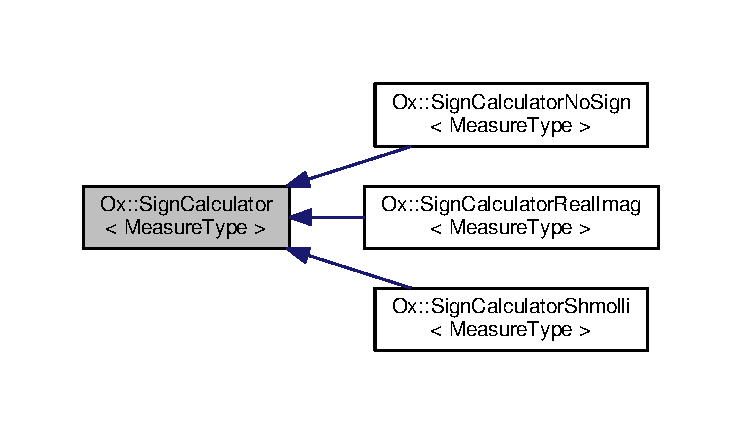
\includegraphics[width=350pt]{class_ox_1_1_sign_calculator__inherit__graph}
\end{center}
\end{figure}
\subsection*{Public Member Functions}
\begin{DoxyCompactItemize}
\item 
virtual const Measure\+Type $\ast$ {\bfseries get\+Inv\+Times} () const \hypertarget{class_ox_1_1_sign_calculator_aeae2b269b870b515f9da0ecb9a0c9dda}{}\label{class_ox_1_1_sign_calculator_aeae2b269b870b515f9da0ecb9a0c9dda}

\item 
virtual const Measure\+Type $\ast$ {\bfseries get\+Sig\+Mag} () const \hypertarget{class_ox_1_1_sign_calculator_abe5cfb287faab9e06e113bf33daa9b2e}{}\label{class_ox_1_1_sign_calculator_abe5cfb287faab9e06e113bf33daa9b2e}

\item 
virtual const Measure\+Type $\ast$ {\bfseries get\+Sig\+Pha} () const \hypertarget{class_ox_1_1_sign_calculator_a5d875d51f77739c61d8c6391d665ade9}{}\label{class_ox_1_1_sign_calculator_a5d875d51f77739c61d8c6391d665ade9}

\item 
virtual Measure\+Type $\ast$ {\bfseries get\+Signal} ()\hypertarget{class_ox_1_1_sign_calculator_ac4dc2ae5e3e5eee88d0a3a347a68a637}{}\label{class_ox_1_1_sign_calculator_ac4dc2ae5e3e5eee88d0a3a347a68a637}

\item 
virtual Measure\+Type $\ast$ {\bfseries get\+Signs} ()\hypertarget{class_ox_1_1_sign_calculator_a04d65630c95cf94ee6198193a5c0c346}{}\label{class_ox_1_1_sign_calculator_a04d65630c95cf94ee6198193a5c0c346}

\item 
virtual int {\bfseries get\+N\+Samples} ()\hypertarget{class_ox_1_1_sign_calculator_a6f1f77383cd088a1339ae91ce0b58e40}{}\label{class_ox_1_1_sign_calculator_a6f1f77383cd088a1339ae91ce0b58e40}

\item 
virtual void {\bfseries set\+Inv\+Times} (const Measure\+Type $\ast$\+\_\+\+Inv\+Times)\hypertarget{class_ox_1_1_sign_calculator_a184b9d2bd4b6677fef960aef40dbfe1c}{}\label{class_ox_1_1_sign_calculator_a184b9d2bd4b6677fef960aef40dbfe1c}

\item 
virtual void {\bfseries set\+Sig\+Mag} (const Measure\+Type $\ast$\+\_\+\+Sig\+Mag)\hypertarget{class_ox_1_1_sign_calculator_ad010dcfd41f343b7d9cad99a3c628468}{}\label{class_ox_1_1_sign_calculator_ad010dcfd41f343b7d9cad99a3c628468}

\item 
virtual void {\bfseries set\+Sig\+Pha} (const Measure\+Type $\ast$\+\_\+\+Sig\+Pha)\hypertarget{class_ox_1_1_sign_calculator_a1fe78e188915e35e8d0db885642852c9}{}\label{class_ox_1_1_sign_calculator_a1fe78e188915e35e8d0db885642852c9}

\item 
virtual void {\bfseries set\+Signal} (Measure\+Type $\ast$\+\_\+\+Signal)\hypertarget{class_ox_1_1_sign_calculator_ade6aa249b05f92357cb825065be8a203}{}\label{class_ox_1_1_sign_calculator_ade6aa249b05f92357cb825065be8a203}

\item 
virtual void {\bfseries set\+Signs} (Measure\+Type $\ast$\+\_\+\+Signs)\hypertarget{class_ox_1_1_sign_calculator_a3de14f899f64c93df9076fb837e553bf}{}\label{class_ox_1_1_sign_calculator_a3de14f899f64c93df9076fb837e553bf}

\item 
virtual void {\bfseries set\+N\+Samples} (int \+\_\+n\+Samples)\hypertarget{class_ox_1_1_sign_calculator_a8a4f3f8b94fad53d444cf6f1c1191497}{}\label{class_ox_1_1_sign_calculator_a8a4f3f8b94fad53d444cf6f1c1191497}

\item 
virtual int \hyperlink{class_ox_1_1_sign_calculator_a6a85028b70e41f6a60a5b639c468e455}{calculate\+Sign} ()=0
\item 
virtual void {\bfseries disp} ()\hypertarget{class_ox_1_1_sign_calculator_afc55176ad2a81085942e1e98242376bf}{}\label{class_ox_1_1_sign_calculator_afc55176ad2a81085942e1e98242376bf}

\item 
void \hyperlink{class_ox_1_1_sign_calculator_a59de754f72402b4cf7dc2f8766f0a1ff}{set\+All\+Pointers\+To\+Null} ()\hypertarget{class_ox_1_1_sign_calculator_a59de754f72402b4cf7dc2f8766f0a1ff}{}\label{class_ox_1_1_sign_calculator_a59de754f72402b4cf7dc2f8766f0a1ff}

\begin{DoxyCompactList}\small\item\em set all the pointers to zero \end{DoxyCompactList}\item 
\hyperlink{class_ox_1_1_sign_calculator_a1b0a177a5f2c6080d6730ff5fdc384af}{Sign\+Calculator} ()\hypertarget{class_ox_1_1_sign_calculator_a1b0a177a5f2c6080d6730ff5fdc384af}{}\label{class_ox_1_1_sign_calculator_a1b0a177a5f2c6080d6730ff5fdc384af}

\begin{DoxyCompactList}\small\item\em constructor \end{DoxyCompactList}\item 
\hyperlink{class_ox_1_1_sign_calculator_a118469032ecb643b93ba56f948fdce85}{Sign\+Calculator} (const \hyperlink{class_ox_1_1_sign_calculator}{Sign\+Calculator} \&old)\hypertarget{class_ox_1_1_sign_calculator_a118469032ecb643b93ba56f948fdce85}{}\label{class_ox_1_1_sign_calculator_a118469032ecb643b93ba56f948fdce85}

\begin{DoxyCompactList}\small\item\em copy constructor \end{DoxyCompactList}\item 
virtual \hyperlink{class_ox_1_1_sign_calculator}{Sign\+Calculator}$<$ Measure\+Type $>$ $\ast$ \hyperlink{class_ox_1_1_sign_calculator_a40d9d97a505a69b687429bf545597687}{new\+By\+Cloning} ()=0
\item 
virtual \hyperlink{class_ox_1_1_sign_calculator_a5143a172e360633d8df758756d146889}{$\sim$\+Sign\+Calculator} ()\hypertarget{class_ox_1_1_sign_calculator_a5143a172e360633d8df758756d146889}{}\label{class_ox_1_1_sign_calculator_a5143a172e360633d8df758756d146889}

\begin{DoxyCompactList}\small\item\em do not forget about the virtual destructor, see \href{https://stackoverflow.com/questions/461203/when-to-use-virtual-destructors}{\tt https\+://stackoverflow.\+com/questions/461203/when-\/to-\/use-\/virtual-\/destructors} \end{DoxyCompactList}\end{DoxyCompactItemize}
\subsection*{Protected Attributes}
\begin{DoxyCompactItemize}
\item 
const Measure\+Type $\ast$ {\bfseries \+\_\+\+Inv\+Times}\hypertarget{class_ox_1_1_sign_calculator_a46be35659f793c2e1280a975f799db4d}{}\label{class_ox_1_1_sign_calculator_a46be35659f793c2e1280a975f799db4d}

\item 
const Measure\+Type $\ast$ {\bfseries \+\_\+\+Sig\+Mag}\hypertarget{class_ox_1_1_sign_calculator_a635a62974bc9b9f30d0d560a84fcf3f1}{}\label{class_ox_1_1_sign_calculator_a635a62974bc9b9f30d0d560a84fcf3f1}

\item 
const Measure\+Type $\ast$ {\bfseries \+\_\+\+Sig\+Pha}\hypertarget{class_ox_1_1_sign_calculator_a19b203aacea5e39bc9675a27c57197d3}{}\label{class_ox_1_1_sign_calculator_a19b203aacea5e39bc9675a27c57197d3}

\item 
Measure\+Type $\ast$ {\bfseries \+\_\+\+Signal}\hypertarget{class_ox_1_1_sign_calculator_aaf53cad7c5d49133017677f8abb589bf}{}\label{class_ox_1_1_sign_calculator_aaf53cad7c5d49133017677f8abb589bf}

\item 
Measure\+Type $\ast$ {\bfseries \+\_\+\+Signs}\hypertarget{class_ox_1_1_sign_calculator_a6dda6e1e4d83dd7ad4654f7fd2b44bb3}{}\label{class_ox_1_1_sign_calculator_a6dda6e1e4d83dd7ad4654f7fd2b44bb3}

\item 
int {\bfseries \+\_\+n\+Samples}\hypertarget{class_ox_1_1_sign_calculator_a133488500068bccf0e041d9244a09e02}{}\label{class_ox_1_1_sign_calculator_a133488500068bccf0e041d9244a09e02}

\end{DoxyCompactItemize}


\subsection{Detailed Description}
\subsubsection*{template$<$typename Measure\+Type$>$\\*
class Ox\+::\+Sign\+Calculator$<$ Measure\+Type $>$}


\begin{DoxyTemplParams}{Template Parameters}
{\em Measure\+Type} & \\
\hline
\end{DoxyTemplParams}


\subsection{Member Function Documentation}
\index{Ox\+::\+Sign\+Calculator@{Ox\+::\+Sign\+Calculator}!calculate\+Sign@{calculate\+Sign}}
\index{calculate\+Sign@{calculate\+Sign}!Ox\+::\+Sign\+Calculator@{Ox\+::\+Sign\+Calculator}}
\subsubsection[{\texorpdfstring{calculate\+Sign()=0}{calculateSign()=0}}]{\setlength{\rightskip}{0pt plus 5cm}template$<$typename Measure\+Type$>$ virtual int {\bf Ox\+::\+Sign\+Calculator}$<$ Measure\+Type $>$\+::calculate\+Sign (
\begin{DoxyParamCaption}
{}
\end{DoxyParamCaption}
)\hspace{0.3cm}{\ttfamily [pure virtual]}}\hypertarget{class_ox_1_1_sign_calculator_a6a85028b70e41f6a60a5b639c468e455}{}\label{class_ox_1_1_sign_calculator_a6a85028b70e41f6a60a5b639c468e455}
the most important function of this class \begin{DoxyReturn}{Returns}
success/failure 
\end{DoxyReturn}


Implemented in \hyperlink{class_ox_1_1_sign_calculator_no_sign_a8e78a82d817f66385d1a2140f8ef11d7}{Ox\+::\+Sign\+Calculator\+No\+Sign$<$ Measure\+Type $>$}, \hyperlink{class_ox_1_1_sign_calculator_real_imag_ae3f3c8f8e8ea994da7ad56f4a180cb36}{Ox\+::\+Sign\+Calculator\+Real\+Imag$<$ Measure\+Type $>$}, and \hyperlink{class_ox_1_1_sign_calculator_shmolli_ab981a3a9790976de560609860f455edd}{Ox\+::\+Sign\+Calculator\+Shmolli$<$ Measure\+Type $>$}.

\index{Ox\+::\+Sign\+Calculator@{Ox\+::\+Sign\+Calculator}!new\+By\+Cloning@{new\+By\+Cloning}}
\index{new\+By\+Cloning@{new\+By\+Cloning}!Ox\+::\+Sign\+Calculator@{Ox\+::\+Sign\+Calculator}}
\subsubsection[{\texorpdfstring{new\+By\+Cloning()=0}{newByCloning()=0}}]{\setlength{\rightskip}{0pt plus 5cm}template$<$typename Measure\+Type$>$ virtual {\bf Sign\+Calculator}$<$Measure\+Type$>$$\ast$ {\bf Ox\+::\+Sign\+Calculator}$<$ Measure\+Type $>$\+::new\+By\+Cloning (
\begin{DoxyParamCaption}
{}
\end{DoxyParamCaption}
)\hspace{0.3cm}{\ttfamily [pure virtual]}}\hypertarget{class_ox_1_1_sign_calculator_a40d9d97a505a69b687429bf545597687}{}\label{class_ox_1_1_sign_calculator_a40d9d97a505a69b687429bf545597687}
cloning \begin{DoxyReturn}{Returns}

\end{DoxyReturn}


Implemented in \hyperlink{class_ox_1_1_sign_calculator_shmolli_a9d9cd9b7107e43b4762846f54ff023d4}{Ox\+::\+Sign\+Calculator\+Shmolli$<$ Measure\+Type $>$}, \hyperlink{class_ox_1_1_sign_calculator_no_sign_ac480086ad668ac264393b1b18a926221}{Ox\+::\+Sign\+Calculator\+No\+Sign$<$ Measure\+Type $>$}, and \hyperlink{class_ox_1_1_sign_calculator_real_imag_ae3340d1ac5728efcaf3d5a9299f01f2c}{Ox\+::\+Sign\+Calculator\+Real\+Imag$<$ Measure\+Type $>$}.



The documentation for this class was generated from the following file\+:\begin{DoxyCompactItemize}
\item 
lib/\hyperlink{_ox_sign_calculator_8h}{Ox\+Sign\+Calculator.\+h}\end{DoxyCompactItemize}

\hypertarget{class_ox_1_1_sign_calculator_no_sign}{}\section{Ox\+:\+:Sign\+Calculator\+No\+Sign$<$ Measure\+Type $>$ Class Template Reference}
\label{class_ox_1_1_sign_calculator_no_sign}\index{Ox\+::\+Sign\+Calculator\+No\+Sign$<$ Measure\+Type $>$@{Ox\+::\+Sign\+Calculator\+No\+Sign$<$ Measure\+Type $>$}}


{\ttfamily \#include $<$Ox\+Sign\+Calculator\+No\+Sign.\+h$>$}



Inheritance diagram for Ox\+:\+:Sign\+Calculator\+No\+Sign$<$ Measure\+Type $>$\+:
\nopagebreak
\begin{figure}[H]
\begin{center}
\leavevmode
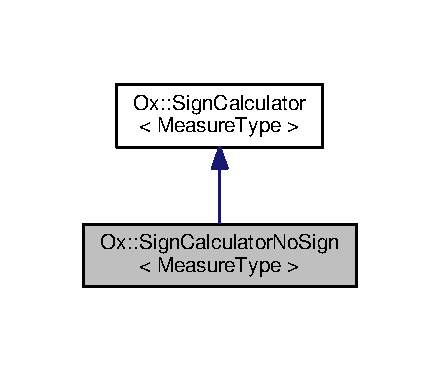
\includegraphics[width=211pt]{class_ox_1_1_sign_calculator_no_sign__inherit__graph}
\end{center}
\end{figure}


Collaboration diagram for Ox\+:\+:Sign\+Calculator\+No\+Sign$<$ Measure\+Type $>$\+:
\nopagebreak
\begin{figure}[H]
\begin{center}
\leavevmode
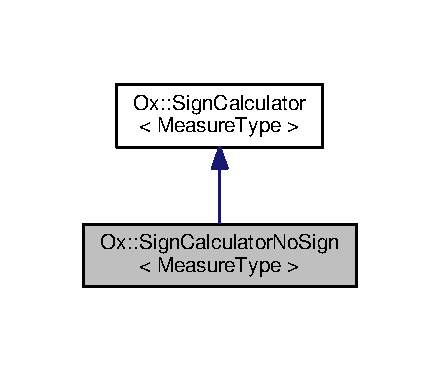
\includegraphics[width=211pt]{class_ox_1_1_sign_calculator_no_sign__coll__graph}
\end{center}
\end{figure}
\subsection*{Public Member Functions}
\begin{DoxyCompactItemize}
\item 
virtual int \hyperlink{class_ox_1_1_sign_calculator_no_sign_a8e78a82d817f66385d1a2140f8ef11d7}{calculate\+Sign} ()
\item 
\hyperlink{class_ox_1_1_sign_calculator_no_sign_ad61e381c257ac4b4f615d94461dc49b1}{Sign\+Calculator\+No\+Sign} ()\hypertarget{class_ox_1_1_sign_calculator_no_sign_ad61e381c257ac4b4f615d94461dc49b1}{}\label{class_ox_1_1_sign_calculator_no_sign_ad61e381c257ac4b4f615d94461dc49b1}

\begin{DoxyCompactList}\small\item\em constructor \end{DoxyCompactList}\item 
\hyperlink{class_ox_1_1_sign_calculator_no_sign_af7d02fdbe8062421741d00f60c9e57aa}{Sign\+Calculator\+No\+Sign} (const \hyperlink{class_ox_1_1_sign_calculator_no_sign}{Sign\+Calculator\+No\+Sign} \&old)\hypertarget{class_ox_1_1_sign_calculator_no_sign_af7d02fdbe8062421741d00f60c9e57aa}{}\label{class_ox_1_1_sign_calculator_no_sign_af7d02fdbe8062421741d00f60c9e57aa}

\begin{DoxyCompactList}\small\item\em copy constructor \end{DoxyCompactList}\item 
virtual \hyperlink{class_ox_1_1_sign_calculator}{Sign\+Calculator}$<$ Measure\+Type $>$ $\ast$ \hyperlink{class_ox_1_1_sign_calculator_no_sign_ac480086ad668ac264393b1b18a926221}{new\+By\+Cloning} ()
\item 
virtual \hyperlink{class_ox_1_1_sign_calculator_no_sign_a1da2b6c351daf89811c6d9618df2bb74}{$\sim$\+Sign\+Calculator\+No\+Sign} ()\hypertarget{class_ox_1_1_sign_calculator_no_sign_a1da2b6c351daf89811c6d9618df2bb74}{}\label{class_ox_1_1_sign_calculator_no_sign_a1da2b6c351daf89811c6d9618df2bb74}

\begin{DoxyCompactList}\small\item\em do not forget about the virtual destructor, see \href{https://stackoverflow.com/questions/461203/when-to-use-virtual-destructors}{\tt https\+://stackoverflow.\+com/questions/461203/when-\/to-\/use-\/virtual-\/destructors} \end{DoxyCompactList}\end{DoxyCompactItemize}
\subsection*{Additional Inherited Members}


\subsection{Detailed Description}
\subsubsection*{template$<$typename Measure\+Type$>$\\*
class Ox\+::\+Sign\+Calculator\+No\+Sign$<$ Measure\+Type $>$}


\begin{DoxyTemplParams}{Template Parameters}
{\em Measure\+Type} & \\
\hline
\end{DoxyTemplParams}


\subsection{Member Function Documentation}
\index{Ox\+::\+Sign\+Calculator\+No\+Sign@{Ox\+::\+Sign\+Calculator\+No\+Sign}!calculate\+Sign@{calculate\+Sign}}
\index{calculate\+Sign@{calculate\+Sign}!Ox\+::\+Sign\+Calculator\+No\+Sign@{Ox\+::\+Sign\+Calculator\+No\+Sign}}
\subsubsection[{\texorpdfstring{calculate\+Sign()}{calculateSign()}}]{\setlength{\rightskip}{0pt plus 5cm}template$<$typename Measure\+Type$>$ virtual int {\bf Ox\+::\+Sign\+Calculator\+No\+Sign}$<$ Measure\+Type $>$\+::calculate\+Sign (
\begin{DoxyParamCaption}
{}
\end{DoxyParamCaption}
)\hspace{0.3cm}{\ttfamily [inline]}, {\ttfamily [virtual]}}\hypertarget{class_ox_1_1_sign_calculator_no_sign_a8e78a82d817f66385d1a2140f8ef11d7}{}\label{class_ox_1_1_sign_calculator_no_sign_a8e78a82d817f66385d1a2140f8ef11d7}
the most important function of this class \begin{DoxyReturn}{Returns}
success/failure 
\end{DoxyReturn}


Implements \hyperlink{class_ox_1_1_sign_calculator_a6a85028b70e41f6a60a5b639c468e455}{Ox\+::\+Sign\+Calculator$<$ Measure\+Type $>$}.

\index{Ox\+::\+Sign\+Calculator\+No\+Sign@{Ox\+::\+Sign\+Calculator\+No\+Sign}!new\+By\+Cloning@{new\+By\+Cloning}}
\index{new\+By\+Cloning@{new\+By\+Cloning}!Ox\+::\+Sign\+Calculator\+No\+Sign@{Ox\+::\+Sign\+Calculator\+No\+Sign}}
\subsubsection[{\texorpdfstring{new\+By\+Cloning()}{newByCloning()}}]{\setlength{\rightskip}{0pt plus 5cm}template$<$typename Measure\+Type$>$ virtual {\bf Sign\+Calculator}$<$Measure\+Type$>$$\ast$ {\bf Ox\+::\+Sign\+Calculator\+No\+Sign}$<$ Measure\+Type $>$\+::new\+By\+Cloning (
\begin{DoxyParamCaption}
{}
\end{DoxyParamCaption}
)\hspace{0.3cm}{\ttfamily [inline]}, {\ttfamily [virtual]}}\hypertarget{class_ox_1_1_sign_calculator_no_sign_ac480086ad668ac264393b1b18a926221}{}\label{class_ox_1_1_sign_calculator_no_sign_ac480086ad668ac264393b1b18a926221}
cloning \begin{DoxyReturn}{Returns}

\end{DoxyReturn}


Implements \hyperlink{class_ox_1_1_sign_calculator_a40d9d97a505a69b687429bf545597687}{Ox\+::\+Sign\+Calculator$<$ Measure\+Type $>$}.



The documentation for this class was generated from the following file\+:\begin{DoxyCompactItemize}
\item 
lib/\hyperlink{_ox_sign_calculator_no_sign_8h}{Ox\+Sign\+Calculator\+No\+Sign.\+h}\end{DoxyCompactItemize}

\hypertarget{class_ox_1_1_sign_calculator_real_imag}{}\section{Ox\+:\+:Sign\+Calculator\+Real\+Imag$<$ Measure\+Type $>$ Class Template Reference}
\label{class_ox_1_1_sign_calculator_real_imag}\index{Ox\+::\+Sign\+Calculator\+Real\+Imag$<$ Measure\+Type $>$@{Ox\+::\+Sign\+Calculator\+Real\+Imag$<$ Measure\+Type $>$}}


{\ttfamily \#include $<$Ox\+Sign\+Calculator\+Real\+Imag.\+h$>$}



Inheritance diagram for Ox\+:\+:Sign\+Calculator\+Real\+Imag$<$ Measure\+Type $>$\+:
\nopagebreak
\begin{figure}[H]
\begin{center}
\leavevmode
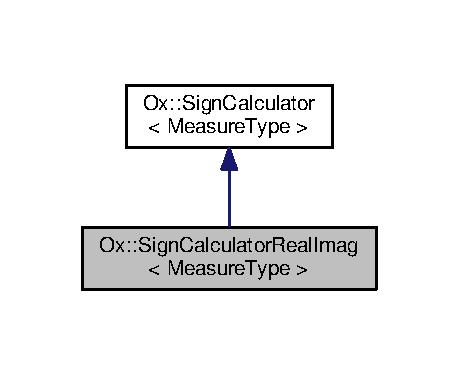
\includegraphics[width=221pt]{class_ox_1_1_sign_calculator_real_imag__inherit__graph}
\end{center}
\end{figure}


Collaboration diagram for Ox\+:\+:Sign\+Calculator\+Real\+Imag$<$ Measure\+Type $>$\+:
\nopagebreak
\begin{figure}[H]
\begin{center}
\leavevmode
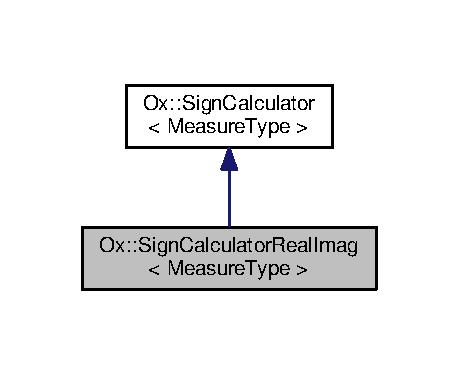
\includegraphics[width=221pt]{class_ox_1_1_sign_calculator_real_imag__coll__graph}
\end{center}
\end{figure}
\subsection*{Public Member Functions}
\begin{DoxyCompactItemize}
\item 
virtual int \hyperlink{class_ox_1_1_sign_calculator_real_imag_ae3f3c8f8e8ea994da7ad56f4a180cb36}{calculate\+Sign} ()
\item 
virtual \hyperlink{class_ox_1_1_sign_calculator}{Sign\+Calculator}$<$ Measure\+Type $>$ $\ast$ \hyperlink{class_ox_1_1_sign_calculator_real_imag_ae3340d1ac5728efcaf3d5a9299f01f2c}{new\+By\+Cloning} ()
\end{DoxyCompactItemize}
\subsection*{Static Public Member Functions}
\begin{DoxyCompactItemize}
\item 
static int {\bfseries Real\+Mag\+Phase2\+Signs} (int n\+Samples, const Measure\+Type $\ast$sig\+Mag, const Measure\+Type $\ast$sig\+Pha, Measure\+Type $\ast$signal, Measure\+Type $\ast$signs)\hypertarget{class_ox_1_1_sign_calculator_real_imag_a916a7be502489b814bd3b147075ae31d}{}\label{class_ox_1_1_sign_calculator_real_imag_a916a7be502489b814bd3b147075ae31d}

\end{DoxyCompactItemize}
\subsection*{Additional Inherited Members}


\subsection{Detailed Description}
\subsubsection*{template$<$typename Measure\+Type$>$\\*
class Ox\+::\+Sign\+Calculator\+Real\+Imag$<$ Measure\+Type $>$}


\begin{DoxyTemplParams}{Template Parameters}
{\em Measure\+Type} & \\
\hline
\end{DoxyTemplParams}


\subsection{Member Function Documentation}
\index{Ox\+::\+Sign\+Calculator\+Real\+Imag@{Ox\+::\+Sign\+Calculator\+Real\+Imag}!calculate\+Sign@{calculate\+Sign}}
\index{calculate\+Sign@{calculate\+Sign}!Ox\+::\+Sign\+Calculator\+Real\+Imag@{Ox\+::\+Sign\+Calculator\+Real\+Imag}}
\subsubsection[{\texorpdfstring{calculate\+Sign()}{calculateSign()}}]{\setlength{\rightskip}{0pt plus 5cm}template$<$typename Measure\+Type$>$ virtual int {\bf Ox\+::\+Sign\+Calculator\+Real\+Imag}$<$ Measure\+Type $>$\+::calculate\+Sign (
\begin{DoxyParamCaption}
{}
\end{DoxyParamCaption}
)\hspace{0.3cm}{\ttfamily [inline]}, {\ttfamily [virtual]}}\hypertarget{class_ox_1_1_sign_calculator_real_imag_ae3f3c8f8e8ea994da7ad56f4a180cb36}{}\label{class_ox_1_1_sign_calculator_real_imag_ae3f3c8f8e8ea994da7ad56f4a180cb36}
the most important function of this class \begin{DoxyReturn}{Returns}
success/failure 
\end{DoxyReturn}


Implements \hyperlink{class_ox_1_1_sign_calculator_a6a85028b70e41f6a60a5b639c468e455}{Ox\+::\+Sign\+Calculator$<$ Measure\+Type $>$}.

\index{Ox\+::\+Sign\+Calculator\+Real\+Imag@{Ox\+::\+Sign\+Calculator\+Real\+Imag}!new\+By\+Cloning@{new\+By\+Cloning}}
\index{new\+By\+Cloning@{new\+By\+Cloning}!Ox\+::\+Sign\+Calculator\+Real\+Imag@{Ox\+::\+Sign\+Calculator\+Real\+Imag}}
\subsubsection[{\texorpdfstring{new\+By\+Cloning()}{newByCloning()}}]{\setlength{\rightskip}{0pt plus 5cm}template$<$typename Measure\+Type$>$ virtual {\bf Sign\+Calculator}$<$Measure\+Type$>$$\ast$ {\bf Ox\+::\+Sign\+Calculator\+Real\+Imag}$<$ Measure\+Type $>$\+::new\+By\+Cloning (
\begin{DoxyParamCaption}
{}
\end{DoxyParamCaption}
)\hspace{0.3cm}{\ttfamily [inline]}, {\ttfamily [virtual]}}\hypertarget{class_ox_1_1_sign_calculator_real_imag_ae3340d1ac5728efcaf3d5a9299f01f2c}{}\label{class_ox_1_1_sign_calculator_real_imag_ae3340d1ac5728efcaf3d5a9299f01f2c}
cloning \begin{DoxyReturn}{Returns}

\end{DoxyReturn}


Implements \hyperlink{class_ox_1_1_sign_calculator_a40d9d97a505a69b687429bf545597687}{Ox\+::\+Sign\+Calculator$<$ Measure\+Type $>$}.



The documentation for this class was generated from the following file\+:\begin{DoxyCompactItemize}
\item 
lib/\hyperlink{_ox_sign_calculator_real_imag_8h}{Ox\+Sign\+Calculator\+Real\+Imag.\+h}\end{DoxyCompactItemize}

\hypertarget{class_ox_1_1_start_point_calculator}{}\section{Ox\+:\+:Start\+Point\+Calculator$<$ Measure\+Type $>$ Class Template Reference}
\label{class_ox_1_1_start_point_calculator}\index{Ox\+::\+Start\+Point\+Calculator$<$ Measure\+Type $>$@{Ox\+::\+Start\+Point\+Calculator$<$ Measure\+Type $>$}}


{\ttfamily \#include $<$Ox\+Start\+Point\+Calculator.\+h$>$}



Inheritance diagram for Ox\+:\+:Start\+Point\+Calculator$<$ Measure\+Type $>$\+:
\nopagebreak
\begin{figure}[H]
\begin{center}
\leavevmode
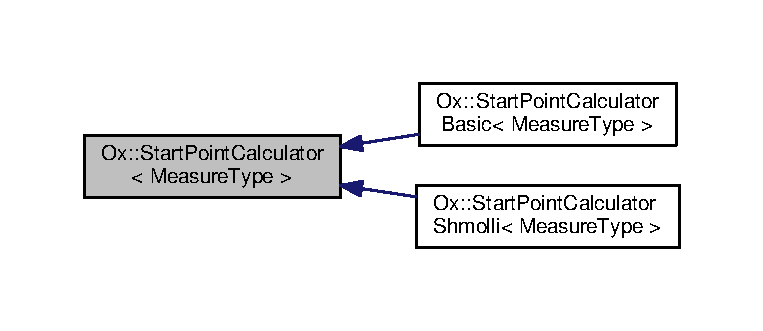
\includegraphics[width=350pt]{class_ox_1_1_start_point_calculator__inherit__graph}
\end{center}
\end{figure}
\subsection*{Public Member Functions}
\begin{DoxyCompactItemize}
\item 
virtual int \hyperlink{class_ox_1_1_start_point_calculator_a9d1132410d68eb16f3f71ec4015c0b2f}{calculate\+Start\+Point} ()=0
\item 
const Measure\+Type $\ast$ {\bfseries get\+Input\+Start\+Point} () const \hypertarget{class_ox_1_1_start_point_calculator_a01bcfb382bec0c4c28ae2bb5783b458c}{}\label{class_ox_1_1_start_point_calculator_a01bcfb382bec0c4c28ae2bb5783b458c}

\item 
Measure\+Type $\ast$ {\bfseries get\+Calculated\+Start\+Point} () const \hypertarget{class_ox_1_1_start_point_calculator_a48b39c1d6bb733821f7297593e424728}{}\label{class_ox_1_1_start_point_calculator_a48b39c1d6bb733821f7297593e424728}

\item 
int {\bfseries get\+N\+Dims} () const \hypertarget{class_ox_1_1_start_point_calculator_a75c73487e21a0f4920762c1efc96d573}{}\label{class_ox_1_1_start_point_calculator_a75c73487e21a0f4920762c1efc96d573}

\item 
virtual void {\bfseries set\+Input\+Start\+Point} (const Measure\+Type $\ast$\+\_\+\+Input\+Start\+Point)\hypertarget{class_ox_1_1_start_point_calculator_ac76047ce4b0d474203cae066471cce61}{}\label{class_ox_1_1_start_point_calculator_ac76047ce4b0d474203cae066471cce61}

\item 
virtual void {\bfseries set\+N\+Dims} (int \+\_\+n\+Dims)\hypertarget{class_ox_1_1_start_point_calculator_a02b51af6d6019cfc47d04b752ad96c86}{}\label{class_ox_1_1_start_point_calculator_a02b51af6d6019cfc47d04b752ad96c86}

\item 
virtual void {\bfseries set\+Inv\+Times} (const Measure\+Type $\ast$\+\_\+\+Inv\+Times)\hypertarget{class_ox_1_1_start_point_calculator_a0632bd0dcf7707930058d63e2176fc7a}{}\label{class_ox_1_1_start_point_calculator_a0632bd0dcf7707930058d63e2176fc7a}

\item 
virtual void {\bfseries set\+Echo\+Times} (const Measure\+Type $\ast$\+\_\+\+Echo\+Times)\hypertarget{class_ox_1_1_start_point_calculator_ab49fe45a4ee7b415edd0948c9fc76fbb}{}\label{class_ox_1_1_start_point_calculator_ab49fe45a4ee7b415edd0948c9fc76fbb}

\item 
virtual void {\bfseries set\+Sig\+Mag} (const Measure\+Type $\ast$\+\_\+\+Sig\+Mag)\hypertarget{class_ox_1_1_start_point_calculator_a7cff5323e92bc00fdc9baa2a3eef7a37}{}\label{class_ox_1_1_start_point_calculator_a7cff5323e92bc00fdc9baa2a3eef7a37}

\item 
virtual void {\bfseries set\+Signs} (const Measure\+Type $\ast$\+\_\+\+Signs)\hypertarget{class_ox_1_1_start_point_calculator_a1245375d6cad369f18ab4a32ddb28446}{}\label{class_ox_1_1_start_point_calculator_a1245375d6cad369f18ab4a32ddb28446}

\item 
virtual void {\bfseries set\+Calculated\+Start\+Point} (Measure\+Type $\ast$\+\_\+\+Calculated\+Start\+Point)\hypertarget{class_ox_1_1_start_point_calculator_aebb0511e802eff920369dec99b6c00fb}{}\label{class_ox_1_1_start_point_calculator_aebb0511e802eff920369dec99b6c00fb}

\item 
virtual void {\bfseries set\+N\+Samples} (int \+\_\+n\+Samples)\hypertarget{class_ox_1_1_start_point_calculator_a72195ac7840734cd9001d0303ab859f4}{}\label{class_ox_1_1_start_point_calculator_a72195ac7840734cd9001d0303ab859f4}

\item 
void {\bfseries disp} ()\hypertarget{class_ox_1_1_start_point_calculator_a1e68d3a23cee006d4dbdd47583c5d316}{}\label{class_ox_1_1_start_point_calculator_a1e68d3a23cee006d4dbdd47583c5d316}

\item 
void \hyperlink{class_ox_1_1_start_point_calculator_a00a48e8845623b57e414380924a3f82b}{set\+All\+Pointers\+To\+Null} ()\hypertarget{class_ox_1_1_start_point_calculator_a00a48e8845623b57e414380924a3f82b}{}\label{class_ox_1_1_start_point_calculator_a00a48e8845623b57e414380924a3f82b}

\begin{DoxyCompactList}\small\item\em set all the pointers to zero \end{DoxyCompactList}\item 
\hyperlink{class_ox_1_1_start_point_calculator_a408ce85b6fbf0ee69f4eca3176b814d6}{Start\+Point\+Calculator} ()\hypertarget{class_ox_1_1_start_point_calculator_a408ce85b6fbf0ee69f4eca3176b814d6}{}\label{class_ox_1_1_start_point_calculator_a408ce85b6fbf0ee69f4eca3176b814d6}

\begin{DoxyCompactList}\small\item\em constructor \end{DoxyCompactList}\item 
\hyperlink{class_ox_1_1_start_point_calculator_ab6b12ed8fa6b47b3335b5c7a92b94623}{Start\+Point\+Calculator} (const \hyperlink{class_ox_1_1_start_point_calculator}{Start\+Point\+Calculator} \&old)\hypertarget{class_ox_1_1_start_point_calculator_ab6b12ed8fa6b47b3335b5c7a92b94623}{}\label{class_ox_1_1_start_point_calculator_ab6b12ed8fa6b47b3335b5c7a92b94623}

\begin{DoxyCompactList}\small\item\em copy constructor \end{DoxyCompactList}\item 
virtual \hyperlink{class_ox_1_1_start_point_calculator}{Start\+Point\+Calculator}$<$ Measure\+Type $>$ $\ast$ \hyperlink{class_ox_1_1_start_point_calculator_acd2a221872002157f232e1e7f73a1859}{new\+By\+Cloning} ()=0
\item 
virtual \hyperlink{class_ox_1_1_start_point_calculator_a210c3312a8926b750dba8e498c6b620a}{$\sim$\+Start\+Point\+Calculator} ()\hypertarget{class_ox_1_1_start_point_calculator_a210c3312a8926b750dba8e498c6b620a}{}\label{class_ox_1_1_start_point_calculator_a210c3312a8926b750dba8e498c6b620a}

\begin{DoxyCompactList}\small\item\em do not forget about the virtual destructor, see \href{https://stackoverflow.com/questions/461203/when-to-use-virtual-destructors}{\tt https\+://stackoverflow.\+com/questions/461203/when-\/to-\/use-\/virtual-\/destructors} \end{DoxyCompactList}\end{DoxyCompactItemize}
\subsection*{Protected Attributes}
\begin{DoxyCompactItemize}
\item 
Measure\+Type $\ast$ {\bfseries \+\_\+\+Input\+Start\+Point}\hypertarget{class_ox_1_1_start_point_calculator_a92176ada269bb53017ed3cbedb3b629d}{}\label{class_ox_1_1_start_point_calculator_a92176ada269bb53017ed3cbedb3b629d}

\item 
Measure\+Type $\ast$ {\bfseries \+\_\+\+Calculated\+Start\+Point}\hypertarget{class_ox_1_1_start_point_calculator_a90c26143db22a371533de08a87cdada0}{}\label{class_ox_1_1_start_point_calculator_a90c26143db22a371533de08a87cdada0}

\item 
const Measure\+Type $\ast$ {\bfseries \+\_\+\+Inv\+Times}\hypertarget{class_ox_1_1_start_point_calculator_a64929ca24726ddf99017b6f18cc03e29}{}\label{class_ox_1_1_start_point_calculator_a64929ca24726ddf99017b6f18cc03e29}

\item 
const Measure\+Type $\ast$ {\bfseries \+\_\+\+Echo\+Times}\hypertarget{class_ox_1_1_start_point_calculator_a7549a2a735665d8b204c230c817fc5d4}{}\label{class_ox_1_1_start_point_calculator_a7549a2a735665d8b204c230c817fc5d4}

\item 
const Measure\+Type $\ast$ {\bfseries \+\_\+\+Sig\+Mag}\hypertarget{class_ox_1_1_start_point_calculator_a5cf615178da5bb3af984eea616548e05}{}\label{class_ox_1_1_start_point_calculator_a5cf615178da5bb3af984eea616548e05}

\item 
const Measure\+Type $\ast$ {\bfseries \+\_\+\+Signs}\hypertarget{class_ox_1_1_start_point_calculator_abce7ef554368d8739ac27dddb63382df}{}\label{class_ox_1_1_start_point_calculator_abce7ef554368d8739ac27dddb63382df}

\item 
int {\bfseries \+\_\+n\+Samples}\hypertarget{class_ox_1_1_start_point_calculator_a17601c059cd679301597bc897e297c2f}{}\label{class_ox_1_1_start_point_calculator_a17601c059cd679301597bc897e297c2f}

\item 
int {\bfseries \+\_\+n\+Dims}\hypertarget{class_ox_1_1_start_point_calculator_a1bee9378aff7741838dad45ff6d5dc1d}{}\label{class_ox_1_1_start_point_calculator_a1bee9378aff7741838dad45ff6d5dc1d}

\item 
bool {\bfseries \+\_\+n\+Dims\+Changed}\hypertarget{class_ox_1_1_start_point_calculator_a800e7f49b7956602b4ae9e4eb718eadd}{}\label{class_ox_1_1_start_point_calculator_a800e7f49b7956602b4ae9e4eb718eadd}

\end{DoxyCompactItemize}


\subsection{Detailed Description}
\subsubsection*{template$<$typename Measure\+Type$>$\\*
class Ox\+::\+Start\+Point\+Calculator$<$ Measure\+Type $>$}


\begin{DoxyTemplParams}{Template Parameters}
{\em Measure\+Type} & \\
\hline
\end{DoxyTemplParams}


\subsection{Member Function Documentation}
\index{Ox\+::\+Start\+Point\+Calculator@{Ox\+::\+Start\+Point\+Calculator}!calculate\+Start\+Point@{calculate\+Start\+Point}}
\index{calculate\+Start\+Point@{calculate\+Start\+Point}!Ox\+::\+Start\+Point\+Calculator@{Ox\+::\+Start\+Point\+Calculator}}
\subsubsection[{\texorpdfstring{calculate\+Start\+Point()=0}{calculateStartPoint()=0}}]{\setlength{\rightskip}{0pt plus 5cm}template$<$typename Measure\+Type$>$ virtual int {\bf Ox\+::\+Start\+Point\+Calculator}$<$ Measure\+Type $>$\+::calculate\+Start\+Point (
\begin{DoxyParamCaption}
{}
\end{DoxyParamCaption}
)\hspace{0.3cm}{\ttfamily [pure virtual]}}\hypertarget{class_ox_1_1_start_point_calculator_a9d1132410d68eb16f3f71ec4015c0b2f}{}\label{class_ox_1_1_start_point_calculator_a9d1132410d68eb16f3f71ec4015c0b2f}
the most important function of this class \begin{DoxyReturn}{Returns}
success/failure 
\end{DoxyReturn}


Implemented in \hyperlink{class_ox_1_1_start_point_calculator_basic_a9d227adf887f091f180f3e2fd37ab2cc}{Ox\+::\+Start\+Point\+Calculator\+Basic$<$ Measure\+Type $>$}, and \hyperlink{class_ox_1_1_start_point_calculator_shmolli_acd0913906ed0d4301b78b5329cc3d62f}{Ox\+::\+Start\+Point\+Calculator\+Shmolli$<$ Measure\+Type $>$}.

\index{Ox\+::\+Start\+Point\+Calculator@{Ox\+::\+Start\+Point\+Calculator}!new\+By\+Cloning@{new\+By\+Cloning}}
\index{new\+By\+Cloning@{new\+By\+Cloning}!Ox\+::\+Start\+Point\+Calculator@{Ox\+::\+Start\+Point\+Calculator}}
\subsubsection[{\texorpdfstring{new\+By\+Cloning()=0}{newByCloning()=0}}]{\setlength{\rightskip}{0pt plus 5cm}template$<$typename Measure\+Type$>$ virtual {\bf Start\+Point\+Calculator}$<$Measure\+Type$>$$\ast$ {\bf Ox\+::\+Start\+Point\+Calculator}$<$ Measure\+Type $>$\+::new\+By\+Cloning (
\begin{DoxyParamCaption}
{}
\end{DoxyParamCaption}
)\hspace{0.3cm}{\ttfamily [pure virtual]}}\hypertarget{class_ox_1_1_start_point_calculator_acd2a221872002157f232e1e7f73a1859}{}\label{class_ox_1_1_start_point_calculator_acd2a221872002157f232e1e7f73a1859}
cloning \begin{DoxyReturn}{Returns}

\end{DoxyReturn}


Implemented in \hyperlink{class_ox_1_1_start_point_calculator_shmolli_ab3f7f6efa7fb6ac4ce1a93fb7ec42f85}{Ox\+::\+Start\+Point\+Calculator\+Shmolli$<$ Measure\+Type $>$}, and \hyperlink{class_ox_1_1_start_point_calculator_basic_a65bb3460d9358f3d9538648e221c8247}{Ox\+::\+Start\+Point\+Calculator\+Basic$<$ Measure\+Type $>$}.



The documentation for this class was generated from the following file\+:\begin{DoxyCompactItemize}
\item 
lib/\hyperlink{_ox_start_point_calculator_8h}{Ox\+Start\+Point\+Calculator.\+h}\end{DoxyCompactItemize}

\hypertarget{class_ox_1_1_start_point_calculator_default3_dims}{\section{Ox\-:\-:Start\-Point\-Calculator\-Default3\-Dims$<$ Measure\-Type $>$ Class Template Reference}
\label{class_ox_1_1_start_point_calculator_default3_dims}\index{Ox\-::\-Start\-Point\-Calculator\-Default3\-Dims$<$ Measure\-Type $>$@{Ox\-::\-Start\-Point\-Calculator\-Default3\-Dims$<$ Measure\-Type $>$}}
}


{\ttfamily \#include $<$Ox\-Start\-Point\-Calculator\-Default3\-Dims.\-h$>$}



Inheritance diagram for Ox\-:\-:Start\-Point\-Calculator\-Default3\-Dims$<$ Measure\-Type $>$\-:
\nopagebreak
\begin{figure}[H]
\begin{center}
\leavevmode
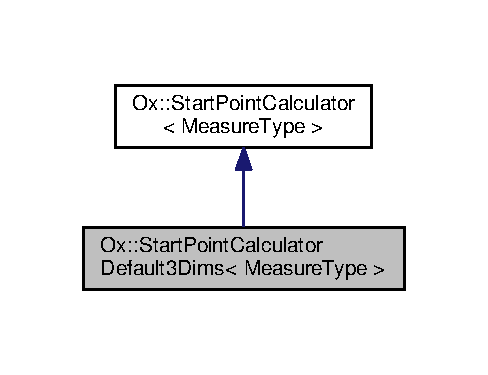
\includegraphics[width=234pt]{class_ox_1_1_start_point_calculator_default3_dims__inherit__graph}
\end{center}
\end{figure}


Collaboration diagram for Ox\-:\-:Start\-Point\-Calculator\-Default3\-Dims$<$ Measure\-Type $>$\-:
\nopagebreak
\begin{figure}[H]
\begin{center}
\leavevmode
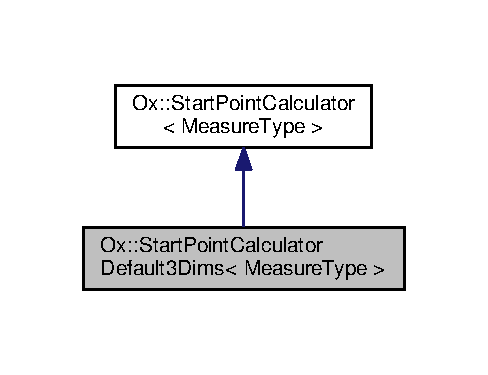
\includegraphics[width=234pt]{class_ox_1_1_start_point_calculator_default3_dims__coll__graph}
\end{center}
\end{figure}
\subsection*{Public Member Functions}
\begin{DoxyCompactItemize}
\item 
virtual int \hyperlink{class_ox_1_1_start_point_calculator_default3_dims_a6af87ac3412f699ebf9abec6b61461cf}{calculate\-Start\-Point} ()
\item 
\hypertarget{class_ox_1_1_start_point_calculator_default3_dims_a87a616c2a07d07684874cf3ab16cb81a}{int {\bfseries set\-Start\-Point\-To\-Default} ()}\label{class_ox_1_1_start_point_calculator_default3_dims_a87a616c2a07d07684874cf3ab16cb81a}

\item 
\hypertarget{class_ox_1_1_start_point_calculator_default3_dims_ae5c36c3bf882f4770613e5e67821d97b}{\hyperlink{class_ox_1_1_start_point_calculator_default3_dims_ae5c36c3bf882f4770613e5e67821d97b}{Start\-Point\-Calculator\-Default3\-Dims} ()}\label{class_ox_1_1_start_point_calculator_default3_dims_ae5c36c3bf882f4770613e5e67821d97b}

\begin{DoxyCompactList}\small\item\em constructor \end{DoxyCompactList}\item 
\hypertarget{class_ox_1_1_start_point_calculator_default3_dims_a915d5b061b445db983c03d671c65e799}{\hyperlink{class_ox_1_1_start_point_calculator_default3_dims_a915d5b061b445db983c03d671c65e799}{Start\-Point\-Calculator\-Default3\-Dims} (const \hyperlink{class_ox_1_1_start_point_calculator_default3_dims}{Start\-Point\-Calculator\-Default3\-Dims} \&old)}\label{class_ox_1_1_start_point_calculator_default3_dims_a915d5b061b445db983c03d671c65e799}

\begin{DoxyCompactList}\small\item\em copy constructor \end{DoxyCompactList}\item 
virtual \hyperlink{class_ox_1_1_start_point_calculator}{Start\-Point\-Calculator}\\*
$<$ Measure\-Type $>$ $\ast$ \hyperlink{class_ox_1_1_start_point_calculator_default3_dims_ad2d60ec81810eb5b0368834e15d031bd}{new\-By\-Cloning} ()
\item 
\hypertarget{class_ox_1_1_start_point_calculator_default3_dims_ab85b597c934ed1ac03ff7079bd860b44}{virtual \hyperlink{class_ox_1_1_start_point_calculator_default3_dims_ab85b597c934ed1ac03ff7079bd860b44}{$\sim$\-Start\-Point\-Calculator\-Default3\-Dims} ()}\label{class_ox_1_1_start_point_calculator_default3_dims_ab85b597c934ed1ac03ff7079bd860b44}

\begin{DoxyCompactList}\small\item\em do not forget about the virtual destructor, see \href{https://stackoverflow.com/questions/461203/when-to-use-virtual-destructors}{\tt https\-://stackoverflow.\-com/questions/461203/when-\/to-\/use-\/virtual-\/destructors} \end{DoxyCompactList}\end{DoxyCompactItemize}
\subsection*{Protected Attributes}
\begin{DoxyCompactItemize}
\item 
\hypertarget{class_ox_1_1_start_point_calculator_default3_dims_ae6d2a377bab89b97d728cf638ac64d47}{Measure\-Type {\bfseries \-\_\-\-Default\-Start\-Point} \mbox{[}3\mbox{]}}\label{class_ox_1_1_start_point_calculator_default3_dims_ae6d2a377bab89b97d728cf638ac64d47}

\end{DoxyCompactItemize}


\subsection{Detailed Description}
\subsubsection*{template$<$typename Measure\-Type$>$class Ox\-::\-Start\-Point\-Calculator\-Default3\-Dims$<$ Measure\-Type $>$}


\begin{DoxyTemplParams}{Template Parameters}
{\em Measure\-Type} & \\
\hline
\end{DoxyTemplParams}


\subsection{Member Function Documentation}
\hypertarget{class_ox_1_1_start_point_calculator_default3_dims_a6af87ac3412f699ebf9abec6b61461cf}{\index{Ox\-::\-Start\-Point\-Calculator\-Default3\-Dims@{Ox\-::\-Start\-Point\-Calculator\-Default3\-Dims}!calculate\-Start\-Point@{calculate\-Start\-Point}}
\index{calculate\-Start\-Point@{calculate\-Start\-Point}!Ox::StartPointCalculatorDefault3Dims@{Ox\-::\-Start\-Point\-Calculator\-Default3\-Dims}}
\subsubsection[{calculate\-Start\-Point}]{\setlength{\rightskip}{0pt plus 5cm}template$<$typename Measure\-Type$>$ virtual int {\bf Ox\-::\-Start\-Point\-Calculator\-Default3\-Dims}$<$ Measure\-Type $>$\-::calculate\-Start\-Point (
\begin{DoxyParamCaption}
{}
\end{DoxyParamCaption}
)\hspace{0.3cm}{\ttfamily [inline]}, {\ttfamily [virtual]}}}\label{class_ox_1_1_start_point_calculator_default3_dims_a6af87ac3412f699ebf9abec6b61461cf}
the most important function of this class \begin{DoxyReturn}{Returns}
success/failure 
\end{DoxyReturn}


Implements \hyperlink{class_ox_1_1_start_point_calculator_a9d1132410d68eb16f3f71ec4015c0b2f}{Ox\-::\-Start\-Point\-Calculator$<$ Measure\-Type $>$}.

\hypertarget{class_ox_1_1_start_point_calculator_default3_dims_ad2d60ec81810eb5b0368834e15d031bd}{\index{Ox\-::\-Start\-Point\-Calculator\-Default3\-Dims@{Ox\-::\-Start\-Point\-Calculator\-Default3\-Dims}!new\-By\-Cloning@{new\-By\-Cloning}}
\index{new\-By\-Cloning@{new\-By\-Cloning}!Ox::StartPointCalculatorDefault3Dims@{Ox\-::\-Start\-Point\-Calculator\-Default3\-Dims}}
\subsubsection[{new\-By\-Cloning}]{\setlength{\rightskip}{0pt plus 5cm}template$<$typename Measure\-Type$>$ virtual {\bf Start\-Point\-Calculator}$<$Measure\-Type$>$$\ast$ {\bf Ox\-::\-Start\-Point\-Calculator\-Default3\-Dims}$<$ Measure\-Type $>$\-::new\-By\-Cloning (
\begin{DoxyParamCaption}
{}
\end{DoxyParamCaption}
)\hspace{0.3cm}{\ttfamily [inline]}, {\ttfamily [virtual]}}}\label{class_ox_1_1_start_point_calculator_default3_dims_ad2d60ec81810eb5b0368834e15d031bd}
cloning \begin{DoxyReturn}{Returns}

\end{DoxyReturn}


Implements \hyperlink{class_ox_1_1_start_point_calculator_acd2a221872002157f232e1e7f73a1859}{Ox\-::\-Start\-Point\-Calculator$<$ Measure\-Type $>$}.



The documentation for this class was generated from the following file\-:\begin{DoxyCompactItemize}
\item 
lib/\hyperlink{_ox_start_point_calculator_default3_dims_8h}{Ox\-Start\-Point\-Calculator\-Default3\-Dims.\-h}\end{DoxyCompactItemize}

\hypertarget{class_ox_1_1_test_data}{\section{Ox\-:\-:Test\-Data$<$ Measure\-Type $>$ Class Template Reference}
\label{class_ox_1_1_test_data}\index{Ox\-::\-Test\-Data$<$ Measure\-Type $>$@{Ox\-::\-Test\-Data$<$ Measure\-Type $>$}}
}
\subsection*{Public Member Functions}
\begin{DoxyCompactItemize}
\item 
\hypertarget{class_ox_1_1_test_data_add19d13b8ec2404fc5d6ebf4ee79a231}{{\bfseries Test\-Data} (char $\ast$file\-Path)}\label{class_ox_1_1_test_data_add19d13b8ec2404fc5d6ebf4ee79a231}

\item 
\hypertarget{class_ox_1_1_test_data_a4e75699c035937ff96fa131505870208}{virtual std\-::vector$<$ Measure\-Type $>$ {\bfseries get\-Signal\-Mag} () const }\label{class_ox_1_1_test_data_a4e75699c035937ff96fa131505870208}

\item 
\hypertarget{class_ox_1_1_test_data_a287f28ddb03f9acc694528441b57c375}{virtual std\-::vector$<$ Measure\-Type $>$ {\bfseries get\-Signal\-Pha} () const }\label{class_ox_1_1_test_data_a287f28ddb03f9acc694528441b57c375}

\item 
\hypertarget{class_ox_1_1_test_data_a414b631b105104920740e51dcc4a3948}{virtual std\-::vector$<$ Measure\-Type $>$ {\bfseries get\-Signs} () const }\label{class_ox_1_1_test_data_a414b631b105104920740e51dcc4a3948}

\item 
\hypertarget{class_ox_1_1_test_data_a0dafaca55a2c3d57ff2106b518b3fada}{virtual std\-::vector$<$ Measure\-Type $>$ {\bfseries get\-Signal} () const }\label{class_ox_1_1_test_data_a0dafaca55a2c3d57ff2106b518b3fada}

\item 
\hypertarget{class_ox_1_1_test_data_acec1269baa03bfa45845f94f3bc15abe}{virtual std\-::vector$<$ Measure\-Type $>$ {\bfseries get\-Inv\-Times} () const }\label{class_ox_1_1_test_data_acec1269baa03bfa45845f94f3bc15abe}

\item 
\hypertarget{class_ox_1_1_test_data_a68a2cefeed3da1c1dac7a34256b9d640}{virtual std\-::vector$<$ Measure\-Type $>$ {\bfseries get\-Results\-Molli} () const }\label{class_ox_1_1_test_data_a68a2cefeed3da1c1dac7a34256b9d640}

\item 
\hypertarget{class_ox_1_1_test_data_aece21264e7f357c50e2d157f077127f5}{virtual std\-::vector$<$ Measure\-Type $>$ {\bfseries get\-Results\-Shmolli} () const }\label{class_ox_1_1_test_data_aece21264e7f357c50e2d157f077127f5}

\item 
\hypertarget{class_ox_1_1_test_data_a9f625acf214f62d6cdfee00c924ef9b0}{virtual const Measure\-Type $\ast$ {\bfseries get\-Signal\-Mag\-Ptr} () const }\label{class_ox_1_1_test_data_a9f625acf214f62d6cdfee00c924ef9b0}

\item 
\hypertarget{class_ox_1_1_test_data_aafe59c86537fb24e513443e34f2b506d}{virtual const Measure\-Type $\ast$ {\bfseries get\-Signal\-Pha\-Ptr} () const }\label{class_ox_1_1_test_data_aafe59c86537fb24e513443e34f2b506d}

\item 
\hypertarget{class_ox_1_1_test_data_a98127c877fabc49a7112489e928cda05}{virtual const Measure\-Type $\ast$ {\bfseries get\-Signs\-Ptr} () const }\label{class_ox_1_1_test_data_a98127c877fabc49a7112489e928cda05}

\item 
\hypertarget{class_ox_1_1_test_data_a7c52dbd7292dfafd5e9d95eb9d701e19}{virtual const Measure\-Type $\ast$ {\bfseries get\-Signal\-Ptr} () const }\label{class_ox_1_1_test_data_a7c52dbd7292dfafd5e9d95eb9d701e19}

\item 
\hypertarget{class_ox_1_1_test_data_ad6f19708661e0722df977b8dacbf88e7}{virtual const Measure\-Type $\ast$ {\bfseries get\-Inv\-Times\-Ptr} () const }\label{class_ox_1_1_test_data_ad6f19708661e0722df977b8dacbf88e7}

\item 
\hypertarget{class_ox_1_1_test_data_a1cb0dc25db322b7ba075e0ab7f5d6567}{virtual const Measure\-Type $\ast$ {\bfseries get\-Results\-Molli\-Ptr} () const }\label{class_ox_1_1_test_data_a1cb0dc25db322b7ba075e0ab7f5d6567}

\item 
\hypertarget{class_ox_1_1_test_data_ad822f6946548df6c68cf6cb007030702}{virtual const Measure\-Type $\ast$ {\bfseries get\-Results\-Shmolli\-Ptr} () const }\label{class_ox_1_1_test_data_ad822f6946548df6c68cf6cb007030702}

\item 
\hypertarget{class_ox_1_1_test_data_a93fc01cb722f3cadbaa530068c0079da}{virtual int {\bfseries get\-N\-Samples} () const }\label{class_ox_1_1_test_data_a93fc01cb722f3cadbaa530068c0079da}

\item 
\hypertarget{class_ox_1_1_test_data_a4c5bb0b0296218d61c608a8592900c39}{void {\bfseries copy\-Str\-Vector\-To\-Member\-Vector} (std\-::vector$<$ std\-::string $>$ str\-Vector, std\-::vector$<$ Measure\-Type $>$ \&member\-Vector)}\label{class_ox_1_1_test_data_a4c5bb0b0296218d61c608a8592900c39}

\item 
\hypertarget{class_ox_1_1_test_data_ac19364ea614dad392eefb4dbeb8a7903}{void {\bfseries disp} ()}\label{class_ox_1_1_test_data_ac19364ea614dad392eefb4dbeb8a7903}

\item 
\hypertarget{class_ox_1_1_test_data_a3de0e44dba2bd5e3b7556d662575378a}{{\footnotesize template$<$typename T\-Y\-P\-E $>$ }\\void {\bfseries print\-Vector} (std\-::vector$<$ T\-Y\-P\-E $>$ my\-Vector, std\-::string my\-Vector\-Name)}\label{class_ox_1_1_test_data_a3de0e44dba2bd5e3b7556d662575378a}

\end{DoxyCompactItemize}
\subsection*{Protected Member Functions}
\begin{DoxyCompactItemize}
\item 
\hypertarget{class_ox_1_1_test_data_a014e56191a98df90450c0b6fa2abc45d}{void {\bfseries calc\-Signal} ()}\label{class_ox_1_1_test_data_a014e56191a98df90450c0b6fa2abc45d}

\end{DoxyCompactItemize}
\subsection*{Protected Attributes}
\begin{DoxyCompactItemize}
\item 
\hypertarget{class_ox_1_1_test_data_a41f65fef5fa534f713cb8a229e5ae14d}{int {\bfseries \-\_\-n\-Samples}}\label{class_ox_1_1_test_data_a41f65fef5fa534f713cb8a229e5ae14d}

\item 
\hypertarget{class_ox_1_1_test_data_a180e0158dc204212fd4879690b2ea3ad}{std\-::vector$<$ Measure\-Type $>$ {\bfseries \-\_\-signal\-Mag}}\label{class_ox_1_1_test_data_a180e0158dc204212fd4879690b2ea3ad}

\item 
\hypertarget{class_ox_1_1_test_data_a5012bab7b7943d05b33151aae38efcc1}{std\-::vector$<$ Measure\-Type $>$ {\bfseries \-\_\-signal\-Pha}}\label{class_ox_1_1_test_data_a5012bab7b7943d05b33151aae38efcc1}

\item 
\hypertarget{class_ox_1_1_test_data_a3d844b169fbdbfcb77d5ef0bf527f554}{std\-::vector$<$ Measure\-Type $>$ {\bfseries \-\_\-signal}}\label{class_ox_1_1_test_data_a3d844b169fbdbfcb77d5ef0bf527f554}

\item 
\hypertarget{class_ox_1_1_test_data_a9e22c4f291064b0c49f7c8007e77b40a}{std\-::vector$<$ Measure\-Type $>$ {\bfseries \-\_\-signs}}\label{class_ox_1_1_test_data_a9e22c4f291064b0c49f7c8007e77b40a}

\item 
\hypertarget{class_ox_1_1_test_data_a4a72325aa7d38c4cac1762a47b7eed1a}{std\-::vector$<$ Measure\-Type $>$ {\bfseries \-\_\-inv\-Times}}\label{class_ox_1_1_test_data_a4a72325aa7d38c4cac1762a47b7eed1a}

\item 
\hypertarget{class_ox_1_1_test_data_a91ae0ccd1b9dea3b83bfc4d7c300dbb0}{std\-::vector$<$ Measure\-Type $>$ {\bfseries \-\_\-results\-Molli}}\label{class_ox_1_1_test_data_a91ae0ccd1b9dea3b83bfc4d7c300dbb0}

\item 
\hypertarget{class_ox_1_1_test_data_ac549cebd93bd96747a68e3680442adfd}{std\-::vector$<$ Measure\-Type $>$ {\bfseries \-\_\-results\-Shmolli}}\label{class_ox_1_1_test_data_ac549cebd93bd96747a68e3680442adfd}

\end{DoxyCompactItemize}


The documentation for this class was generated from the following files\-:\begin{DoxyCompactItemize}
\item 
tests/\hyperlink{_ox_test_data_8h}{Ox\-Test\-Data.\-h}\item 
tests/\hyperlink{_ox_test_data_8hxx}{Ox\-Test\-Data.\-hxx}\end{DoxyCompactItemize}

\hypertarget{class_ox_1_1_test_image}{\section{Ox\-:\-:Test\-Image$<$ Measure\-Type $>$ Class Template Reference}
\label{class_ox_1_1_test_image}\index{Ox\-::\-Test\-Image$<$ Measure\-Type $>$@{Ox\-::\-Test\-Image$<$ Measure\-Type $>$}}
}
\subsection*{Public Member Functions}
\begin{DoxyCompactItemize}
\item 
\hypertarget{class_ox_1_1_test_image_a3b5ceff06d34b2ebd4a4ff215e156088}{{\bfseries Test\-Image} (int n\-Cols, int n\-Rows, std\-::vector$<$ std\-::string $>$ files\-Paths, std\-::vector$<$ int $>$ inv\-Times\-Order)}\label{class_ox_1_1_test_image_a3b5ceff06d34b2ebd4a4ff215e156088}

\item 
\hypertarget{class_ox_1_1_test_image_a794b321a180a2b19d88efc316e0d47aa}{{\bfseries Test\-Image} (int n\-Cols, int n\-Rows, std\-::vector$<$ std\-::string $>$ files\-Paths)}\label{class_ox_1_1_test_image_a794b321a180a2b19d88efc316e0d47aa}

\item 
\hypertarget{class_ox_1_1_test_image_aa802ece1484e88fd748b462c6e2a6cf9}{int {\bfseries init} (int n\-Cols, int n\-Rows, std\-::vector$<$ std\-::string $>$ files\-Paths, std\-::vector$<$ int $>$ inv\-Times\-Order)}\label{class_ox_1_1_test_image_aa802ece1484e88fd748b462c6e2a6cf9}

\item 
\hypertarget{class_ox_1_1_test_image_a6dda2e0b1c2f9d285a29007a14441be3}{virtual Measure\-Type $\ast$ {\bfseries get\-Inv\-Times\-Ptr} ()}\label{class_ox_1_1_test_image_a6dda2e0b1c2f9d285a29007a14441be3}

\item 
\hypertarget{class_ox_1_1_test_image_accd975ba34db53a323810f506e0953d1}{virtual std\-::vector$<$ Measure\-Type $>$ {\bfseries get\-Inv\-Times} () const }\label{class_ox_1_1_test_image_accd975ba34db53a323810f506e0953d1}

\item 
\hypertarget{class_ox_1_1_test_image_a825435d601877f1595b5b04d8f2df2c1}{virtual Measure\-Type $\ast$ {\bfseries get\-Image\-Mag\-Ptr} () const }\label{class_ox_1_1_test_image_a825435d601877f1595b5b04d8f2df2c1}

\item 
\hypertarget{class_ox_1_1_test_image_a6e7c4c1195dfd0c1938c913b230b48a7}{virtual Measure\-Type $\ast$ {\bfseries get\-Image\-Pha\-Ptr} () const }\label{class_ox_1_1_test_image_a6e7c4c1195dfd0c1938c913b230b48a7}

\item 
\hypertarget{class_ox_1_1_test_image_a9da80782972a99cae274cde3de03bbda}{virtual Measure\-Type $\ast$ {\bfseries get\-Image\-Results\-Molli\-Ptr} () const }\label{class_ox_1_1_test_image_a9da80782972a99cae274cde3de03bbda}

\item 
\hypertarget{class_ox_1_1_test_image_aef09efd3eb4b1a37d3b6b479d1e4a016}{virtual Measure\-Type $\ast$ {\bfseries get\-Image\-Results\-Shmolli\-Ptr} () const }\label{class_ox_1_1_test_image_aef09efd3eb4b1a37d3b6b479d1e4a016}

\item 
\hypertarget{class_ox_1_1_test_image_af5a9aadf12db9fdff87ed6aff4e0a2ef}{virtual int {\bfseries get\-N\-Cols} () const }\label{class_ox_1_1_test_image_af5a9aadf12db9fdff87ed6aff4e0a2ef}

\item 
\hypertarget{class_ox_1_1_test_image_acdc29d077640af69c4caac7c60d31cd6}{virtual int {\bfseries get\-N\-Rows} () const }\label{class_ox_1_1_test_image_acdc29d077640af69c4caac7c60d31cd6}

\item 
\hypertarget{class_ox_1_1_test_image_a87559c865b1f365c0bd7cfc9c5939d2b}{virtual int {\bfseries get\-N\-Samples} () const }\label{class_ox_1_1_test_image_a87559c865b1f365c0bd7cfc9c5939d2b}

\end{DoxyCompactItemize}
\subsection*{Protected Attributes}
\begin{DoxyCompactItemize}
\item 
\hypertarget{class_ox_1_1_test_image_aede6d17394f5b1d7aee6287c17482bed}{int {\bfseries \-\_\-n\-Cols}}\label{class_ox_1_1_test_image_aede6d17394f5b1d7aee6287c17482bed}

\item 
\hypertarget{class_ox_1_1_test_image_a2fca989633ec429545fefe579641eeb3}{int {\bfseries \-\_\-n\-Rows}}\label{class_ox_1_1_test_image_a2fca989633ec429545fefe579641eeb3}

\item 
\hypertarget{class_ox_1_1_test_image_a0b2de27b3ba5865c071a754c34e86bc7}{int {\bfseries \-\_\-n\-Samples}}\label{class_ox_1_1_test_image_a0b2de27b3ba5865c071a754c34e86bc7}

\item 
\hypertarget{class_ox_1_1_test_image_a9a3283dccb1476d113836134c3479328}{std\-::vector$<$ Measure\-Type $>$ {\bfseries \-\_\-inv\-Times}}\label{class_ox_1_1_test_image_a9a3283dccb1476d113836134c3479328}

\item 
\hypertarget{class_ox_1_1_test_image_aa7d94bb56b584ccae5619fcf5e55218c}{std\-::vector$<$ int $>$ {\bfseries \-\_\-inv\-Times\-Order}}\label{class_ox_1_1_test_image_aa7d94bb56b584ccae5619fcf5e55218c}

\item 
\hypertarget{class_ox_1_1_test_image_aa6d8862446566b0f1bc313de05cedd28}{Measure\-Type $\ast$ {\bfseries \-\_\-image\-Mag}}\label{class_ox_1_1_test_image_aa6d8862446566b0f1bc313de05cedd28}

\item 
\hypertarget{class_ox_1_1_test_image_a108ccefc1c986d4ad3265ec5601841c5}{Measure\-Type $\ast$ {\bfseries \-\_\-image\-Pha}}\label{class_ox_1_1_test_image_a108ccefc1c986d4ad3265ec5601841c5}

\item 
\hypertarget{class_ox_1_1_test_image_aa942d21740af38bc720db46a77fcea6c}{Measure\-Type $\ast$ {\bfseries \-\_\-image\-Results\-Molli}}\label{class_ox_1_1_test_image_aa942d21740af38bc720db46a77fcea6c}

\item 
\hypertarget{class_ox_1_1_test_image_abab3b898dade1792c251df511357be13}{Measure\-Type $\ast$ {\bfseries \-\_\-image\-Results\-Shmolli}}\label{class_ox_1_1_test_image_abab3b898dade1792c251df511357be13}

\end{DoxyCompactItemize}


The documentation for this class was generated from the following files\-:\begin{DoxyCompactItemize}
\item 
tests/\hyperlink{_ox_test_image_8h}{Ox\-Test\-Image.\-h}\item 
tests/\hyperlink{_ox_test_image_8hxx}{Ox\-Test\-Image.\-hxx}\end{DoxyCompactItemize}

\hypertarget{struct_ox_1_1_tomato_options}{\section{Ox\-:\-:Tomato\-Options$<$ T\-Y\-P\-E $>$ Struct Template Reference}
\label{struct_ox_1_1_tomato_options}\index{Ox\-::\-Tomato\-Options$<$ T\-Y\-P\-E $>$@{Ox\-::\-Tomato\-Options$<$ T\-Y\-P\-E $>$}}
}


{\ttfamily \#include $<$Ox\-Factory\-Of\-Fitters.\-h$>$}

\subsection*{Public Member Functions}
\begin{DoxyCompactItemize}
\item 
void \hyperlink{struct_ox_1_1_tomato_options_a76497b53cadad720af7ff0f83b99096b}{init} ()
\item 
\hyperlink{struct_ox_1_1_tomato_options_a974a7659d7eaefe712b1bb00cbd46a93}{Tomato\-Options} ()
\item 
\hyperlink{struct_ox_1_1_tomato_options_abd502ef8966b09c671e2b7a5b565ce38}{Tomato\-Options} (std\-::string file\-Path)
\item 
\hypertarget{struct_ox_1_1_tomato_options_a9630620338003eb675fdfe242449c915}{int {\bfseries find\-In\-Array} (int size, const char $\ast$name\-Array\mbox{[}$\,$\mbox{]}, std\-::string name)}\label{struct_ox_1_1_tomato_options_a9630620338003eb675fdfe242449c915}

\item 
\hypertarget{struct_ox_1_1_tomato_options_ab50a9d1d7044fa64878b9b7141fd4c81}{void {\bfseries print\-Current} ()}\label{struct_ox_1_1_tomato_options_ab50a9d1d7044fa64878b9b7141fd4c81}

\item 
\hypertarget{struct_ox_1_1_tomato_options_a8c763b89efcc2122205363a7e743afa9}{int {\bfseries export\-To\-Yaml} ()}\label{struct_ox_1_1_tomato_options_a8c763b89efcc2122205363a7e743afa9}

\item 
\hypertarget{struct_ox_1_1_tomato_options_a858797a020bbb2504cfcf389bec9bca2}{int {\bfseries export\-To\-Yaml} (std\-::string file\-Path)}\label{struct_ox_1_1_tomato_options_a858797a020bbb2504cfcf389bec9bca2}

\end{DoxyCompactItemize}
\subsection*{Public Attributes}
\begin{DoxyCompactItemize}
\item 
\hypertarget{struct_ox_1_1_tomato_options_ad123055506ec1c4c73b397a5f771d2e7}{std\-::vector$<$ std\-::string $>$ {\bfseries files\-\_\-magnitude}}\label{struct_ox_1_1_tomato_options_ad123055506ec1c4c73b397a5f771d2e7}

\item 
\hypertarget{struct_ox_1_1_tomato_options_acd13f26343647d05164a33cb5b4163f3}{std\-::vector$<$ std\-::string $>$ {\bfseries files\-\_\-phase}}\label{struct_ox_1_1_tomato_options_acd13f26343647d05164a33cb5b4163f3}

\item 
\hypertarget{struct_ox_1_1_tomato_options_aeffcb3fc69397596ce852699a2f3b05d}{std\-::string {\bfseries dir\-\_\-magnitude}}\label{struct_ox_1_1_tomato_options_aeffcb3fc69397596ce852699a2f3b05d}

\item 
\hypertarget{struct_ox_1_1_tomato_options_a92cabcc150b94b5b4c3dbea6e8ecb846}{std\-::string {\bfseries dir\-\_\-phase}}\label{struct_ox_1_1_tomato_options_a92cabcc150b94b5b4c3dbea6e8ecb846}

\item 
\hypertarget{struct_ox_1_1_tomato_options_af31a50b6e23004912a1512812c823a29}{std\-::string {\bfseries dir\-\_\-output\-\_\-map}}\label{struct_ox_1_1_tomato_options_af31a50b6e23004912a1512812c823a29}

\item 
\hypertarget{struct_ox_1_1_tomato_options_ab8e2816968affd97a0ba0b13c44c4c02}{std\-::string {\bfseries dir\-\_\-output\-\_\-fitparams}}\label{struct_ox_1_1_tomato_options_ab8e2816968affd97a0ba0b13c44c4c02}

\item 
\hypertarget{struct_ox_1_1_tomato_options_a0d4ad4476a8817e68ead08d1b0645033}{calculators\-Type\-\_\-t {\bfseries parameter\-\_\-to\-\_\-map}}\label{struct_ox_1_1_tomato_options_a0d4ad4476a8817e68ead08d1b0645033}

\item 
\hypertarget{struct_ox_1_1_tomato_options_a2d1d2149185ef71968980cf8c6afcf14}{fitters\-Type\-\_\-t {\bfseries fitting\-\_\-method}}\label{struct_ox_1_1_tomato_options_a2d1d2149185ef71968980cf8c6afcf14}

\item 
\hypertarget{struct_ox_1_1_tomato_options_aced156934915e4bb658d9f8433f69ee2}{functions\-Type\-\_\-t {\bfseries functions\-\_\-type}}\label{struct_ox_1_1_tomato_options_aced156934915e4bb658d9f8433f69ee2}

\item 
\hypertarget{struct_ox_1_1_tomato_options_a2cf923d6d04fb8cb510db2623e93119d}{sign\-Calculators\-Type\-\_\-t {\bfseries sign\-\_\-calc\-\_\-method}}\label{struct_ox_1_1_tomato_options_a2cf923d6d04fb8cb510db2623e93119d}

\item 
\hypertarget{struct_ox_1_1_tomato_options_a9da2993961d10c848b0860284900c869}{start\-Point\-Calculators\-Type\-\_\-t {\bfseries start\-\_\-point\-\_\-calc\-\_\-method}}\label{struct_ox_1_1_tomato_options_a9da2993961d10c848b0860284900c869}

\item 
\hypertarget{struct_ox_1_1_tomato_options_ae2ac4c46e46b4d183c6944771701040b}{Measure\-Type {\bfseries f\-Tolerance}}\label{struct_ox_1_1_tomato_options_ae2ac4c46e46b4d183c6944771701040b}

\item 
\hypertarget{struct_ox_1_1_tomato_options_a9b864c01b6b0b4e4d5a56470f6c5f004}{int {\bfseries max\-\_\-function\-\_\-evals}}\label{struct_ox_1_1_tomato_options_a9b864c01b6b0b4e4d5a56470f6c5f004}

\item 
\hypertarget{struct_ox_1_1_tomato_options_a367c540e5413f8ffa3a6bc6ef5781b45}{bool {\bfseries use\-\_\-gradient}}\label{struct_ox_1_1_tomato_options_a367c540e5413f8ffa3a6bc6ef5781b45}

\item 
\hypertarget{struct_ox_1_1_tomato_options_af81d1a55409036109d253b313d59e972}{Measure\-Type {\bfseries mean\-\_\-cut\-\_\-off}}\label{struct_ox_1_1_tomato_options_af81d1a55409036109d253b313d59e972}

\item 
\hypertarget{struct_ox_1_1_tomato_options_ab245e10cf32b36c48d66208a5f505099}{Measure\-Type {\bfseries map\-\_\-scale\-\_\-factor}}\label{struct_ox_1_1_tomato_options_ab245e10cf32b36c48d66208a5f505099}

\item 
\hypertarget{struct_ox_1_1_tomato_options_aa762826a11ff767aa969bd66c29b577f}{bool {\bfseries use\-\_\-colorbar}}\label{struct_ox_1_1_tomato_options_aa762826a11ff767aa969bd66c29b577f}

\item 
\hypertarget{struct_ox_1_1_tomato_options_a54efb4945f2857ee4ed9e1d5552fc3dd}{int {\bfseries number\-\_\-of\-\_\-threads}}\label{struct_ox_1_1_tomato_options_a54efb4945f2857ee4ed9e1d5552fc3dd}

\item 
\hypertarget{struct_ox_1_1_tomato_options_a043a4cf0e29a4482406e95f27ab2f860}{bool {\bfseries visualise}}\label{struct_ox_1_1_tomato_options_a043a4cf0e29a4482406e95f27ab2f860}

\item 
\hypertarget{struct_ox_1_1_tomato_options_ab20a779c5a8dd371ec9356e3f9ce79c9}{int {\bfseries output\-\_\-map\-\_\-series\-\_\-number}}\label{struct_ox_1_1_tomato_options_ab20a779c5a8dd371ec9356e3f9ce79c9}

\item 
\hypertarget{struct_ox_1_1_tomato_options_a58664e816cde6eff746bd5abe4fe2d1c}{int {\bfseries output\-\_\-fitparams\-\_\-series\-\_\-number}}\label{struct_ox_1_1_tomato_options_a58664e816cde6eff746bd5abe4fe2d1c}

\item 
\hypertarget{struct_ox_1_1_tomato_options_a008c932c7d65248d2d82e0e654993384}{double {\bfseries calculation\-\_\-time}}\label{struct_ox_1_1_tomato_options_a008c932c7d65248d2d82e0e654993384}

\end{DoxyCompactItemize}


\subsection{Detailed Description}
\subsubsection*{template$<$typename T\-Y\-P\-E$>$struct Ox\-::\-Tomato\-Options$<$ T\-Y\-P\-E $>$}

Here you can configure different fitting methods 
\begin{DoxyTemplParams}{Template Parameters}
{\em T\-Y\-P\-E} & \\
\hline
\end{DoxyTemplParams}


\subsection{Constructor \& Destructor Documentation}
\hypertarget{struct_ox_1_1_tomato_options_a974a7659d7eaefe712b1bb00cbd46a93}{\index{Ox\-::\-Tomato\-Options@{Ox\-::\-Tomato\-Options}!Tomato\-Options@{Tomato\-Options}}
\index{Tomato\-Options@{Tomato\-Options}!Ox::TomatoOptions@{Ox\-::\-Tomato\-Options}}
\subsubsection[{Tomato\-Options}]{\setlength{\rightskip}{0pt plus 5cm}template$<$typename T\-Y\-P\-E$>$ {\bf Ox\-::\-Tomato\-Options}$<$ T\-Y\-P\-E $>$\-::{\bf Tomato\-Options} (
\begin{DoxyParamCaption}
{}
\end{DoxyParamCaption}
)\hspace{0.3cm}{\ttfamily [inline]}}}\label{struct_ox_1_1_tomato_options_a974a7659d7eaefe712b1bb00cbd46a93}
constructor with defaults \hypertarget{struct_ox_1_1_tomato_options_abd502ef8966b09c671e2b7a5b565ce38}{\index{Ox\-::\-Tomato\-Options@{Ox\-::\-Tomato\-Options}!Tomato\-Options@{Tomato\-Options}}
\index{Tomato\-Options@{Tomato\-Options}!Ox::TomatoOptions@{Ox\-::\-Tomato\-Options}}
\subsubsection[{Tomato\-Options}]{\setlength{\rightskip}{0pt plus 5cm}template$<$typename T\-Y\-P\-E$>$ {\bf Ox\-::\-Tomato\-Options}$<$ T\-Y\-P\-E $>$\-::{\bf Tomato\-Options} (
\begin{DoxyParamCaption}
\item[{std\-::string}]{file\-Path}
\end{DoxyParamCaption}
)\hspace{0.3cm}{\ttfamily [inline]}}}\label{struct_ox_1_1_tomato_options_abd502ef8966b09c671e2b7a5b565ce38}
constructor with parser 
\begin{DoxyParams}{Parameters}
{\em file\-Path} & \\
\hline
\end{DoxyParams}


\subsection{Member Function Documentation}
\hypertarget{struct_ox_1_1_tomato_options_a76497b53cadad720af7ff0f83b99096b}{\index{Ox\-::\-Tomato\-Options@{Ox\-::\-Tomato\-Options}!init@{init}}
\index{init@{init}!Ox::TomatoOptions@{Ox\-::\-Tomato\-Options}}
\subsubsection[{init}]{\setlength{\rightskip}{0pt plus 5cm}template$<$typename T\-Y\-P\-E$>$ void {\bf Ox\-::\-Tomato\-Options}$<$ T\-Y\-P\-E $>$\-::init (
\begin{DoxyParamCaption}
{}
\end{DoxyParamCaption}
)\hspace{0.3cm}{\ttfamily [inline]}}}\label{struct_ox_1_1_tomato_options_a76497b53cadad720af7ff0f83b99096b}
initialise the defaults done this way to work around delegating constructors in cpp98 

The documentation for this struct was generated from the following files\-:\begin{DoxyCompactItemize}
\item 
app/\hyperlink{_ox_factory_of_calculators_8h}{Ox\-Factory\-Of\-Calculators.\-h}\item 
app/\hyperlink{_tomato_options_8h}{Tomato\-Options.\-h}\end{DoxyCompactItemize}

\chapter{File Documentation}
\hypertarget{main_8cpp}{\section{app/main.cpp File Reference}
\label{main_8cpp}\index{app/main.\-cpp@{app/main.\-cpp}}
}


A Documented file with main.  


{\ttfamily \#include $<$iostream$>$}\\*
{\ttfamily \#include \char`\"{}yaml.\-h\char`\"{}}\\*
Include dependency graph for main.\-cpp\-:
\nopagebreak
\begin{figure}[H]
\begin{center}
\leavevmode
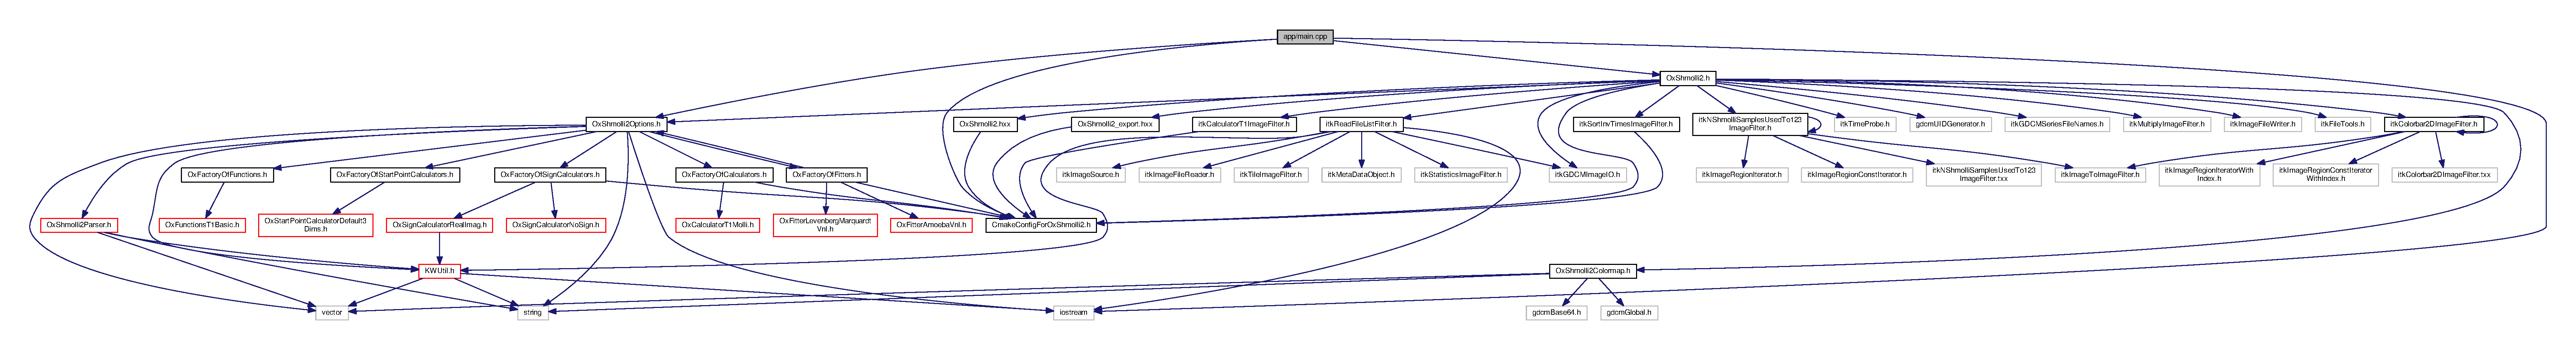
\includegraphics[width=198pt]{main_8cpp__incl}
\end{center}
\end{figure}
\subsection*{Functions}
\begin{DoxyCompactItemize}
\item 
int \hyperlink{main_8cpp_ae66f6b31b5ad750f1fe042a706a4e3d4}{main} ()
\end{DoxyCompactItemize}


\subsection{Detailed Description}
A Documented file with main. Details of the file should be here. \begin{DoxyAuthor}{Author}
Konrad Werys 
\end{DoxyAuthor}
\begin{DoxyDate}{Date}
2018/07/24 
\end{DoxyDate}


\subsection{Function Documentation}
\hypertarget{main_8cpp_ae66f6b31b5ad750f1fe042a706a4e3d4}{\index{main.\-cpp@{main.\-cpp}!main@{main}}
\index{main@{main}!main.cpp@{main.\-cpp}}
\subsubsection[{main}]{\setlength{\rightskip}{0pt plus 5cm}int main (
\begin{DoxyParamCaption}
{}
\end{DoxyParamCaption}
)}}\label{main_8cpp_ae66f6b31b5ad750f1fe042a706a4e3d4}
main \begin{DoxyReturn}{Returns}
always 0 
\end{DoxyReturn}

\hypertarget{_ox_factory_of_calculators_8h}{\section{app/\-Ox\-Factory\-Of\-Calculators.h File Reference}
\label{_ox_factory_of_calculators_8h}\index{app/\-Ox\-Factory\-Of\-Calculators.\-h@{app/\-Ox\-Factory\-Of\-Calculators.\-h}}
}
{\ttfamily \#include \char`\"{}Cmake\-Config\-For\-Tomato.\-h\char`\"{}}\\*
{\ttfamily \#include \char`\"{}Ox\-Calculator\-T1\-Molli.\-h\char`\"{}}\\*
{\ttfamily \#include \char`\"{}Ox\-Calculator\-T1\-Shmolli.\-h\char`\"{}}\\*
{\ttfamily \#include \char`\"{}Ox\-Calculator\-T2.\-h\char`\"{}}\\*
{\ttfamily \#include \char`\"{}Ox\-Calculator\-T2\-Truncation.\-h\char`\"{}}\\*
{\ttfamily \#include \char`\"{}Tomato\-Options.\-h\char`\"{}}\\*
Include dependency graph for Ox\-Factory\-Of\-Calculators.\-h\-:
\nopagebreak
\begin{figure}[H]
\begin{center}
\leavevmode
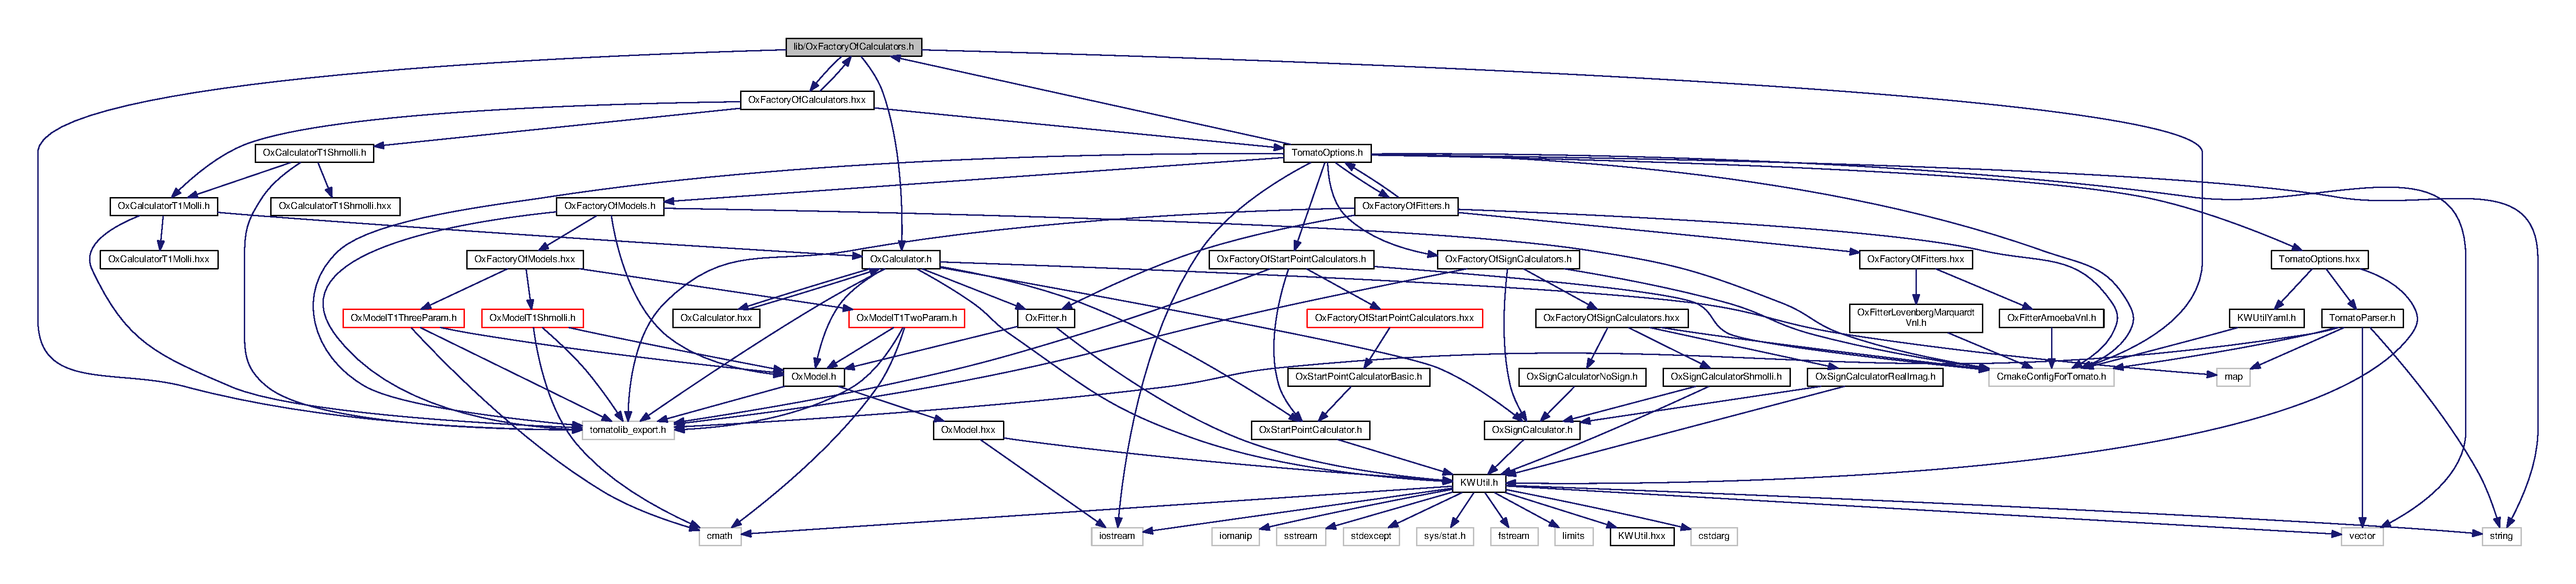
\includegraphics[width=350pt]{_ox_factory_of_calculators_8h__incl}
\end{center}
\end{figure}
This graph shows which files directly or indirectly include this file\-:
\nopagebreak
\begin{figure}[H]
\begin{center}
\leavevmode
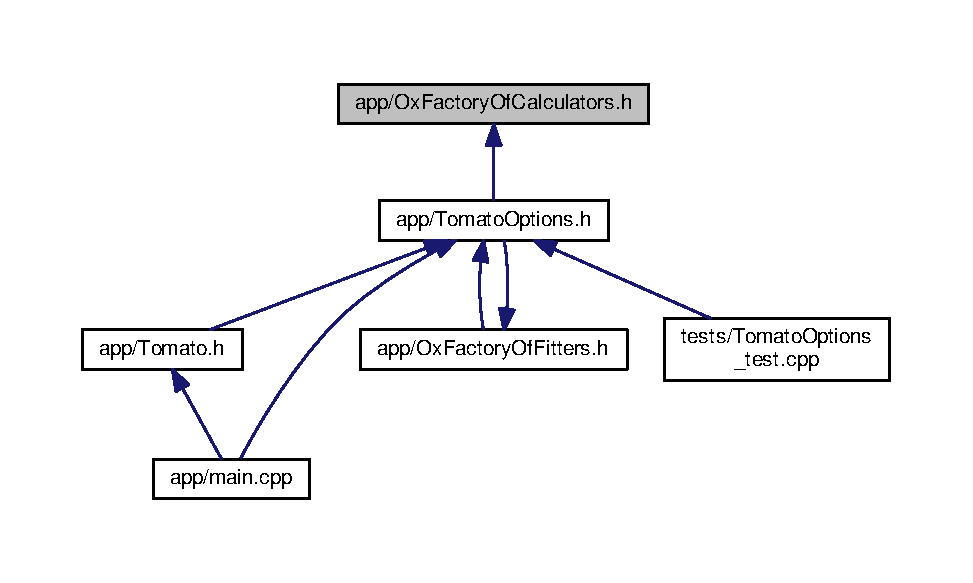
\includegraphics[width=311pt]{_ox_factory_of_calculators_8h__dep__incl}
\end{center}
\end{figure}
\subsection*{Classes}
\begin{DoxyCompactItemize}
\item 
struct \hyperlink{struct_ox_1_1_tomato_options}{Ox\-::\-Tomato\-Options$<$ T\-Y\-P\-E $>$}
\item 
class \hyperlink{class_ox_1_1_factory_of_calculators}{Ox\-::\-Factory\-Of\-Calculators$<$ T\-Y\-P\-E $>$}
\end{DoxyCompactItemize}
\subsection*{Enumerations}
\begin{DoxyCompactItemize}
\item 
enum {\bfseries param\-Type\-\_\-t} \{ {\bfseries T1} = 0, 
{\bfseries T2} = 1, 
{\bfseries T2star} = 2, 
{\bfseries Perf} = 3
 \}
\item 
enum {\bfseries calculators\-Type\-\_\-t} \{ \\*
{\bfseries T1\-\_\-\-M\-O\-L\-L\-I} = 0, 
{\bfseries T1\-\_\-\-S\-H\-M\-O\-L\-L\-I} = 1, 
{\bfseries T1\-\_\-\-S\-H\-M\-O\-L\-L\-I\-\_\-original} = 2, 
{\bfseries T2\-\_\-basic} = 3, 
\\*
{\bfseries T2\-\_\-truncation} = 4, 
{\bfseries last\-Calculator\-Type} = T2\-\_\-truncation
 \}
\end{DoxyCompactItemize}


\subsection{Detailed Description}
\begin{DoxyAuthor}{Author}
Konrad Werys 
\end{DoxyAuthor}
\begin{DoxyDate}{Date}
2018/08/18 
\end{DoxyDate}

\hypertarget{_ox_factory_of_fitters_8h}{\section{app/\-Ox\-Factory\-Of\-Fitters.h File Reference}
\label{_ox_factory_of_fitters_8h}\index{app/\-Ox\-Factory\-Of\-Fitters.\-h@{app/\-Ox\-Factory\-Of\-Fitters.\-h}}
}
{\ttfamily \#include \char`\"{}Cmake\-Config\-For\-Tomato.\-h\char`\"{}}\\*
{\ttfamily \#include \char`\"{}Tomato\-Options.\-h\char`\"{}}\\*
{\ttfamily \#include \char`\"{}Ox\-Fitter\-Amoeba\-Vnl.\-h\char`\"{}}\\*
{\ttfamily \#include \char`\"{}Ox\-Fitter\-Levenberg\-Marquardt\-Vnl.\-h\char`\"{}}\\*
Include dependency graph for Ox\-Factory\-Of\-Fitters.\-h\-:
\nopagebreak
\begin{figure}[H]
\begin{center}
\leavevmode
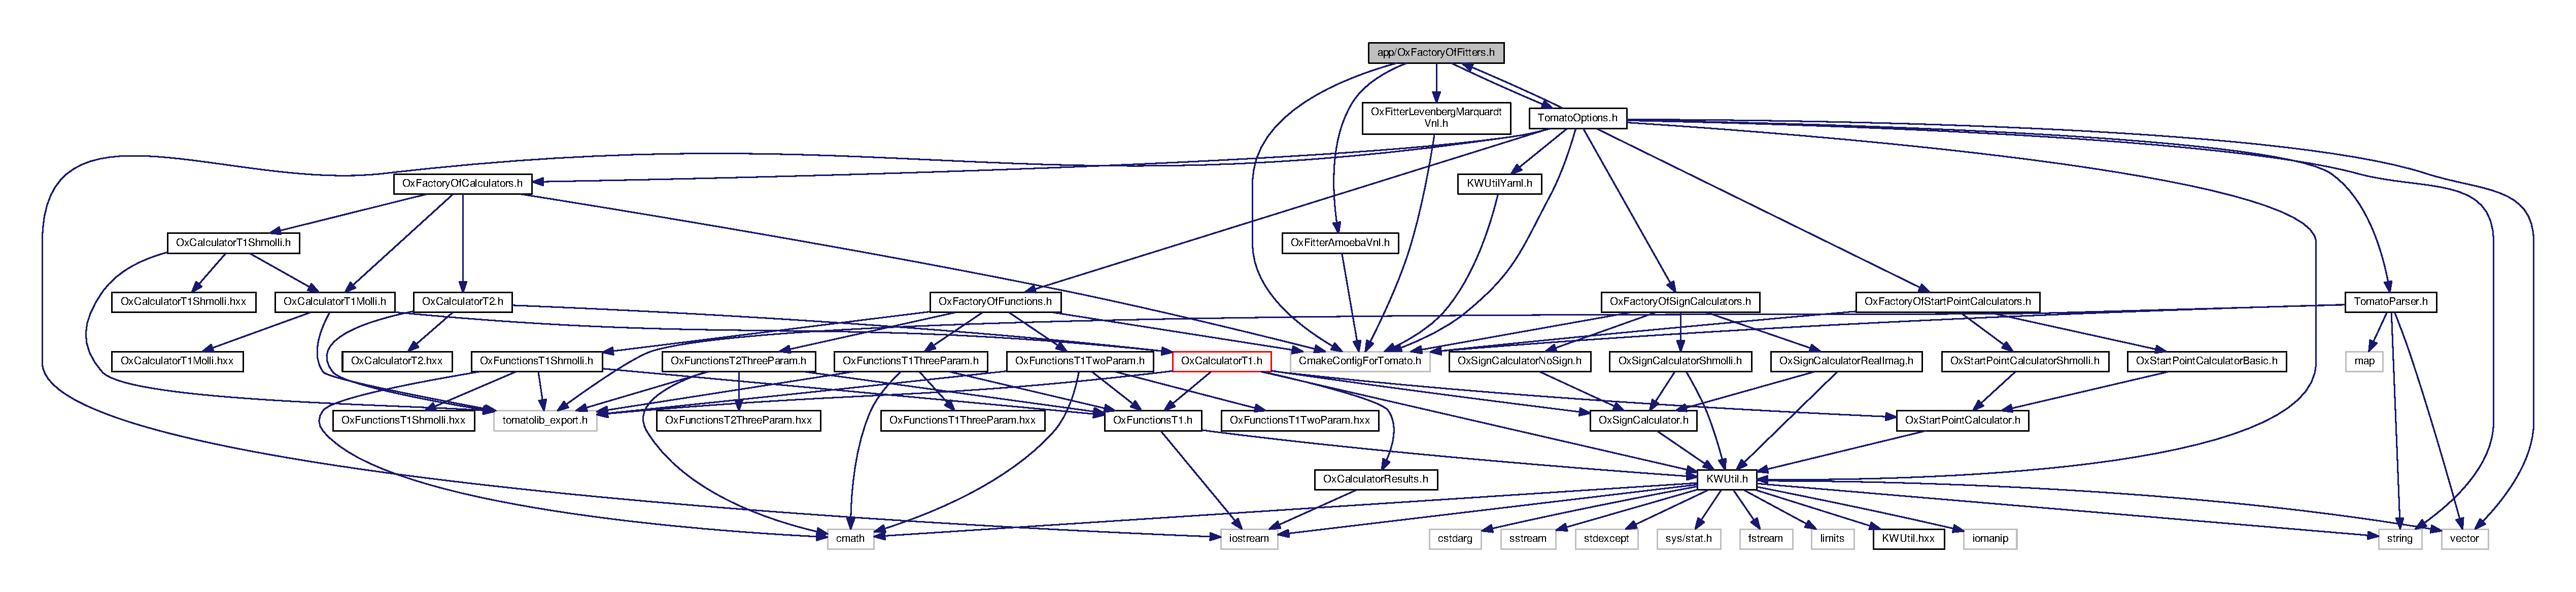
\includegraphics[width=350pt]{_ox_factory_of_fitters_8h__incl}
\end{center}
\end{figure}
This graph shows which files directly or indirectly include this file\-:
\nopagebreak
\begin{figure}[H]
\begin{center}
\leavevmode
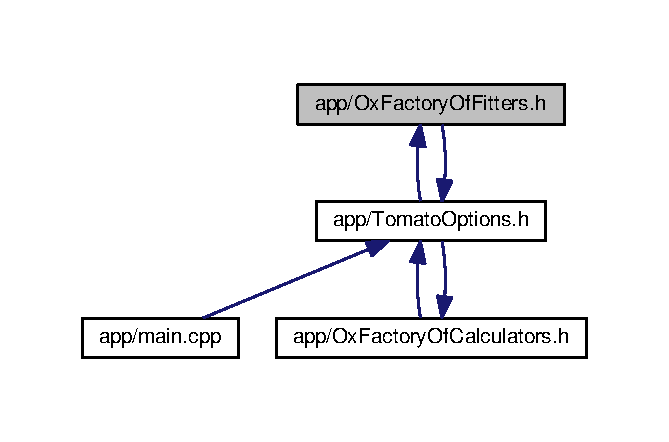
\includegraphics[width=215pt]{_ox_factory_of_fitters_8h__dep__incl}
\end{center}
\end{figure}
\subsection*{Classes}
\begin{DoxyCompactItemize}
\item 
struct \hyperlink{struct_ox_1_1_tomato_options}{Ox\-::\-Tomato\-Options$<$ T\-Y\-P\-E $>$}
\item 
class \hyperlink{class_ox_1_1_factory_of_fitters}{Ox\-::\-Factory\-Of\-Fitters$<$ T\-Y\-P\-E $>$}
\end{DoxyCompactItemize}
\subsection*{Enumerations}
\begin{DoxyCompactItemize}
\item 
enum {\bfseries fitters\-Type\-\_\-t} \{ {\bfseries Amoeba\-Vnl} = 0, 
{\bfseries Lev\-Mar\-Vnl} = 1, 
{\bfseries last\-Fitter\-Type} = Lev\-Mar\-Vnl
 \}
\end{DoxyCompactItemize}


\subsection{Detailed Description}
\begin{DoxyAuthor}{Author}
Konrad Werys 
\end{DoxyAuthor}
\begin{DoxyDate}{Date}
2018/08/18 
\end{DoxyDate}

\hypertarget{_ox_factory_of_functions_8h}{\section{app/\-Ox\-Factory\-Of\-Functions.h File Reference}
\label{_ox_factory_of_functions_8h}\index{app/\-Ox\-Factory\-Of\-Functions.\-h@{app/\-Ox\-Factory\-Of\-Functions.\-h}}
}
{\ttfamily \#include \char`\"{}Cmake\-Config\-For\-Tomato.\-h\char`\"{}}\\*
{\ttfamily \#include \char`\"{}Ox\-Functions\-T1\-Basic.\-h\char`\"{}}\\*
{\ttfamily \#include \char`\"{}Ox\-Functions\-T1\-Shmolli.\-h\char`\"{}}\\*
Include dependency graph for Ox\-Factory\-Of\-Functions.\-h\-:
\nopagebreak
\begin{figure}[H]
\begin{center}
\leavevmode
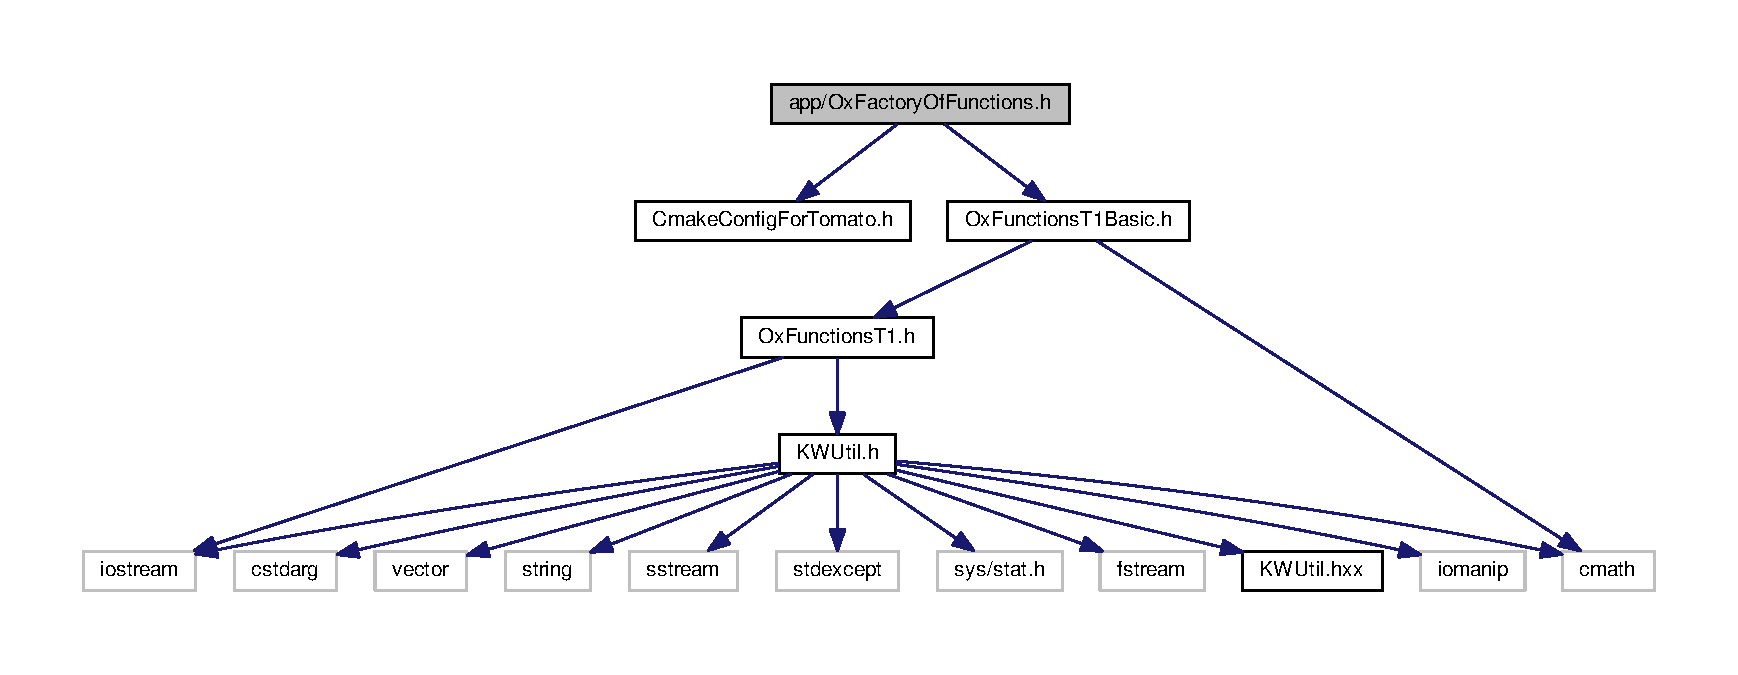
\includegraphics[width=350pt]{_ox_factory_of_functions_8h__incl}
\end{center}
\end{figure}
This graph shows which files directly or indirectly include this file\-:
\nopagebreak
\begin{figure}[H]
\begin{center}
\leavevmode
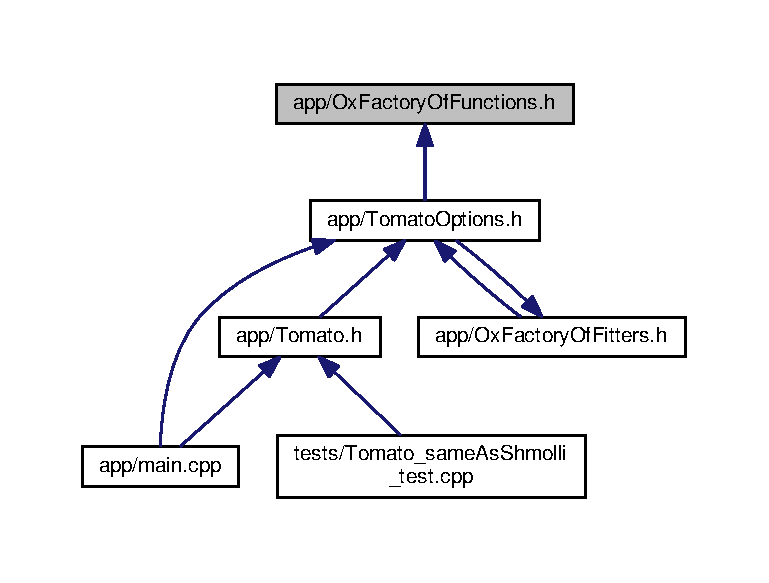
\includegraphics[width=308pt]{_ox_factory_of_functions_8h__dep__incl}
\end{center}
\end{figure}
\subsection*{Classes}
\begin{DoxyCompactItemize}
\item 
struct \hyperlink{struct_ox_1_1_tomato_options}{Ox\-::\-Tomato\-Options$<$ T\-Y\-P\-E $>$}
\item 
class \hyperlink{class_ox_1_1_factory_of_functions}{Ox\-::\-Factory\-Of\-Functions$<$ T\-Y\-P\-E $>$}
\end{DoxyCompactItemize}
\subsection*{Enumerations}
\begin{DoxyCompactItemize}
\item 
enum {\bfseries functions\-Type\-\_\-t} \{ {\bfseries Functions\-Basic} = 0, 
{\bfseries last\-Functor\-Type} = Functions\-Basic
 \}
\end{DoxyCompactItemize}


\subsection{Detailed Description}
\begin{DoxyAuthor}{Author}
Konrad Werys 
\end{DoxyAuthor}
\begin{DoxyDate}{Date}
2018/08/18 
\end{DoxyDate}

\hypertarget{_ox_factory_of_sign_calculators_8h}{\section{app/\-Ox\-Factory\-Of\-Sign\-Calculators.h File Reference}
\label{_ox_factory_of_sign_calculators_8h}\index{app/\-Ox\-Factory\-Of\-Sign\-Calculators.\-h@{app/\-Ox\-Factory\-Of\-Sign\-Calculators.\-h}}
}
{\ttfamily \#include \char`\"{}Cmake\-Config\-For\-Tomato.\-h\char`\"{}}\\*
{\ttfamily \#include \char`\"{}Ox\-Sign\-Calculator\-No\-Sign.\-h\char`\"{}}\\*
{\ttfamily \#include \char`\"{}Ox\-Sign\-Calculator\-Real\-Imag.\-h\char`\"{}}\\*
Include dependency graph for Ox\-Factory\-Of\-Sign\-Calculators.\-h\-:
\nopagebreak
\begin{figure}[H]
\begin{center}
\leavevmode
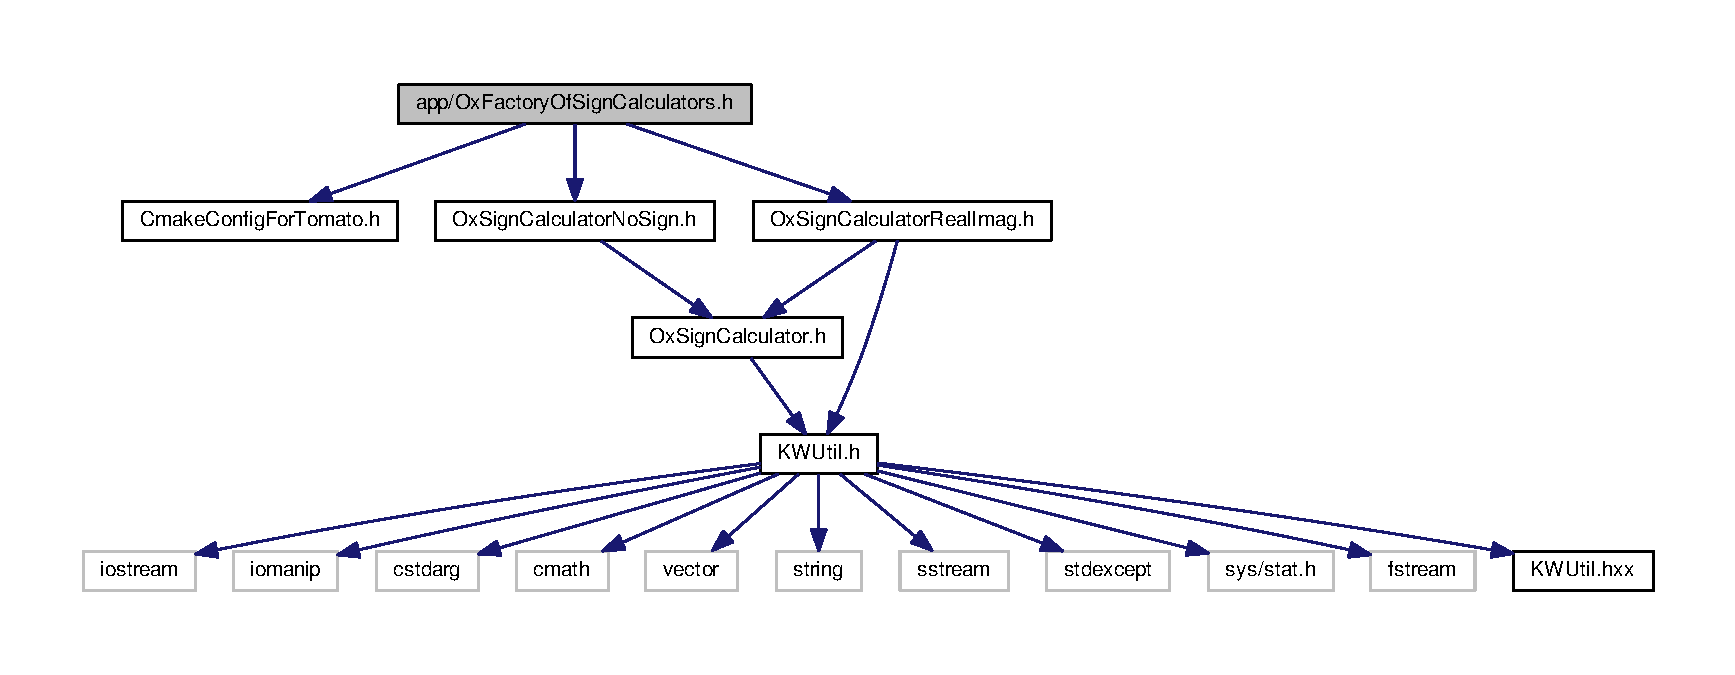
\includegraphics[width=350pt]{_ox_factory_of_sign_calculators_8h__incl}
\end{center}
\end{figure}
This graph shows which files directly or indirectly include this file\-:
\nopagebreak
\begin{figure}[H]
\begin{center}
\leavevmode
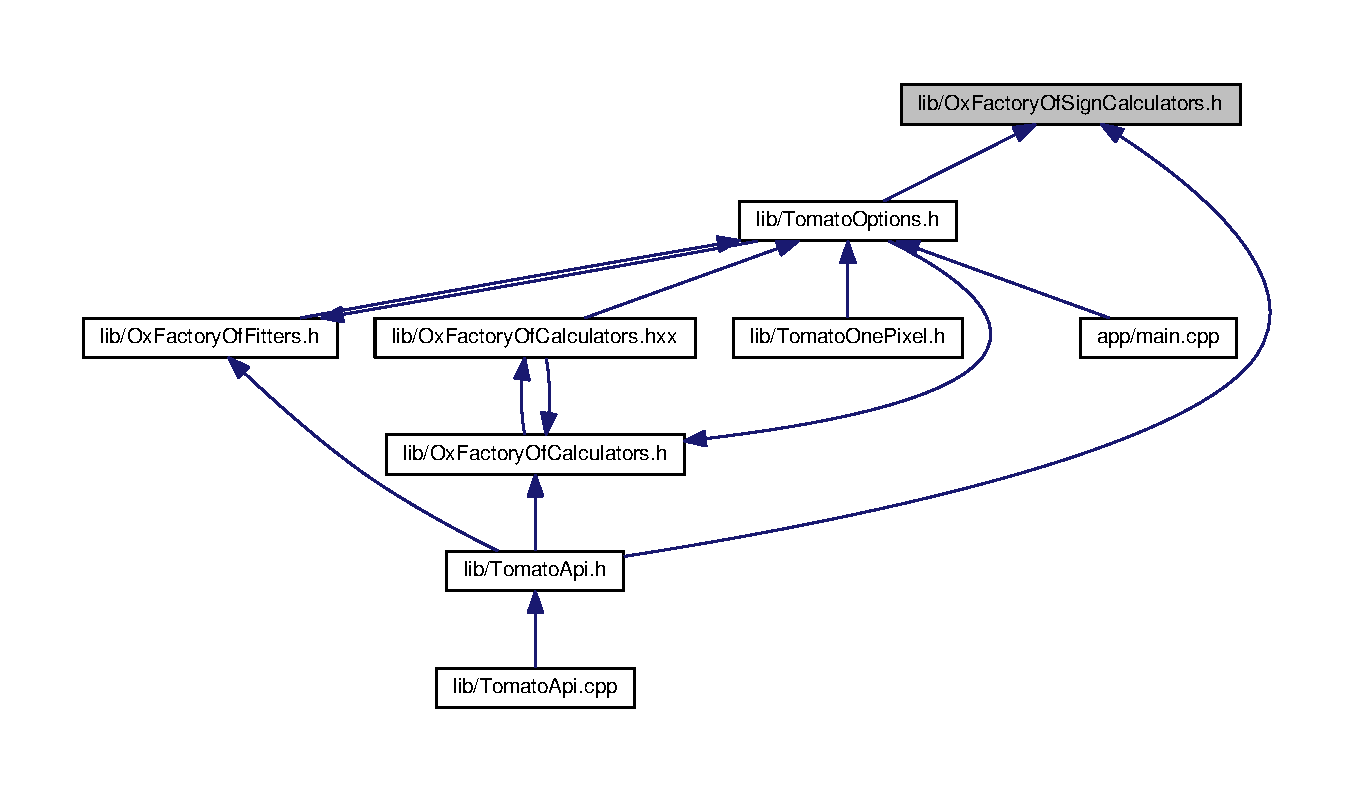
\includegraphics[width=321pt]{_ox_factory_of_sign_calculators_8h__dep__incl}
\end{center}
\end{figure}
\subsection*{Classes}
\begin{DoxyCompactItemize}
\item 
struct \hyperlink{struct_ox_1_1_tomato_options}{Ox\-::\-Tomato\-Options$<$ T\-Y\-P\-E $>$}
\item 
class \hyperlink{class_ox_1_1_factory_of_sign_calculators}{Ox\-::\-Factory\-Of\-Sign\-Calculators$<$ T\-Y\-P\-E $>$}
\end{DoxyCompactItemize}
\subsection*{Enumerations}
\begin{DoxyCompactItemize}
\item 
enum {\bfseries sign\-Calculators\-Type\-\_\-t} \{ {\bfseries No\-Sign} = 0, 
{\bfseries Real\-Imag} = 1, 
{\bfseries last\-Sign\-Calculator\-Type} = Real\-Imag
 \}
\end{DoxyCompactItemize}


\subsection{Detailed Description}
\begin{DoxyAuthor}{Author}
Konrad Werys 
\end{DoxyAuthor}
\begin{DoxyDate}{Date}
2018/08/18 
\end{DoxyDate}

\hypertarget{_ox_factory_of_start_point_calculators_8h}{}\section{lib/\+Ox\+Factory\+Of\+Start\+Point\+Calculators.h File Reference}
\label{_ox_factory_of_start_point_calculators_8h}\index{lib/\+Ox\+Factory\+Of\+Start\+Point\+Calculators.\+h@{lib/\+Ox\+Factory\+Of\+Start\+Point\+Calculators.\+h}}
{\ttfamily \#include \char`\"{}Cmake\+Config\+For\+Tomato.\+h\char`\"{}}\\*
{\ttfamily \#include \char`\"{}tomatolib\+\_\+export.\+h\char`\"{}}\\*
{\ttfamily \#include \char`\"{}Ox\+Start\+Point\+Calculator.\+h\char`\"{}}\\*
{\ttfamily \#include \char`\"{}Ox\+Factory\+Of\+Start\+Point\+Calculators.\+hxx\char`\"{}}\\*
Include dependency graph for Ox\+Factory\+Of\+Start\+Point\+Calculators.\+h\+:
\nopagebreak
\begin{figure}[H]
\begin{center}
\leavevmode
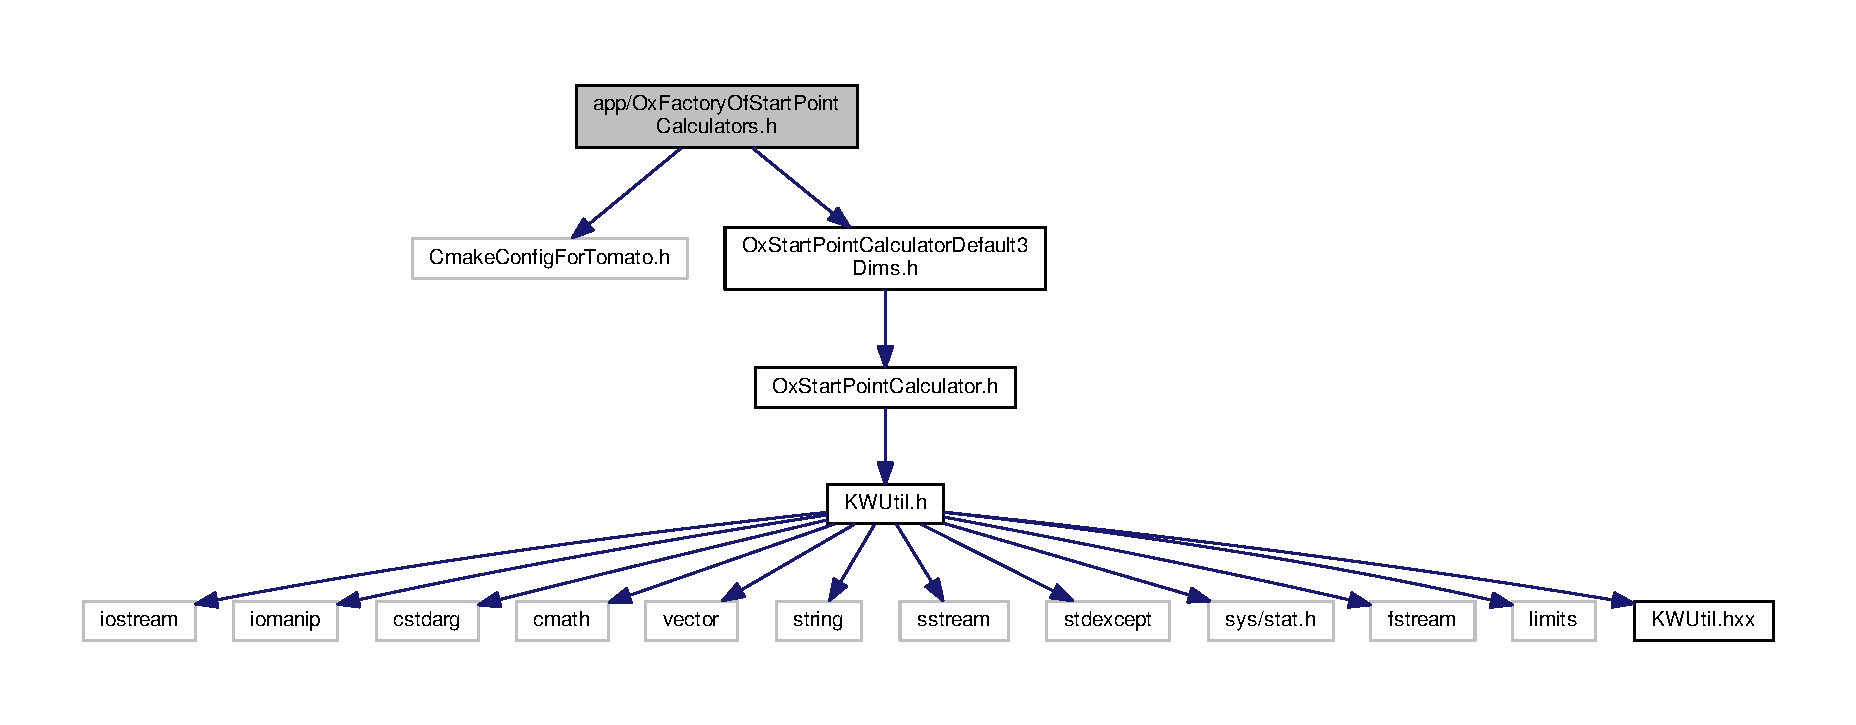
\includegraphics[width=350pt]{_ox_factory_of_start_point_calculators_8h__incl}
\end{center}
\end{figure}
This graph shows which files directly or indirectly include this file\+:
\nopagebreak
\begin{figure}[H]
\begin{center}
\leavevmode
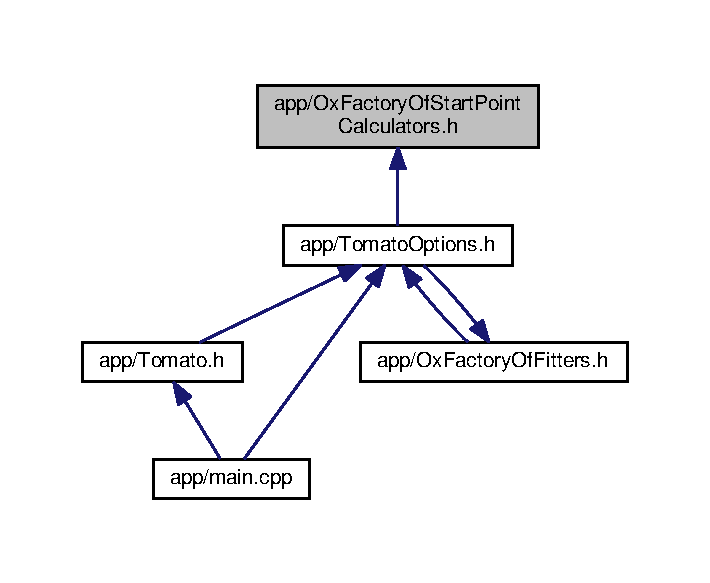
\includegraphics[width=350pt]{_ox_factory_of_start_point_calculators_8h__dep__incl}
\end{center}
\end{figure}
\subsection*{Classes}
\begin{DoxyCompactItemize}
\item 
class \hyperlink{class_ox_1_1_tomato_options}{Ox\+::\+Tomato\+Options$<$ Measure\+Type $>$}
\item 
class \hyperlink{class_ox_1_1_factory_of_start_point_calculators}{Ox\+::\+Factory\+Of\+Start\+Point\+Calculators$<$ T\+Y\+P\+E $>$}
\end{DoxyCompactItemize}
\subsection*{Enumerations}
\begin{DoxyCompactItemize}
\item 
enum {\bfseries start\+Point\+Calculators\+Type\+\_\+t} \{ {\bfseries Basic} = 0, 
{\bfseries Start\+Point\+S\+H\+M\+O\+L\+LI} = 1, 
{\bfseries No\+Start\+Point\+Calculators} = 2, 
{\bfseries last\+Start\+Point\+Calculator\+Type} = No\+Start\+Point\+Calculators
 \}\hypertarget{_ox_factory_of_start_point_calculators_8h_a50e0c7b888ecc4ab3505049584d879b1}{}\label{_ox_factory_of_start_point_calculators_8h_a50e0c7b888ecc4ab3505049584d879b1}

\end{DoxyCompactItemize}


\subsection{Detailed Description}
\begin{DoxyAuthor}{Author}
Konrad Werys 
\end{DoxyAuthor}
\begin{DoxyDate}{Date}
2018/08/18 
\end{DoxyDate}

\hypertarget{_ox_original_shmolli_dicom_reader_8h}{\section{app/\-Ox\-Original\-Shmolli\-Dicom\-Reader.h File Reference}
\label{_ox_original_shmolli_dicom_reader_8h}\index{app/\-Ox\-Original\-Shmolli\-Dicom\-Reader.\-h@{app/\-Ox\-Original\-Shmolli\-Dicom\-Reader.\-h}}
}
{\ttfamily \#include \char`\"{}Cmake\-Config\-For\-Tomato.\-h\char`\"{}}\\*
{\ttfamily \#include \char`\"{}tomatolib\-\_\-export.\-h\char`\"{}}\\*
Include dependency graph for Ox\-Original\-Shmolli\-Dicom\-Reader.\-h\-:
\nopagebreak
\begin{figure}[H]
\begin{center}
\leavevmode
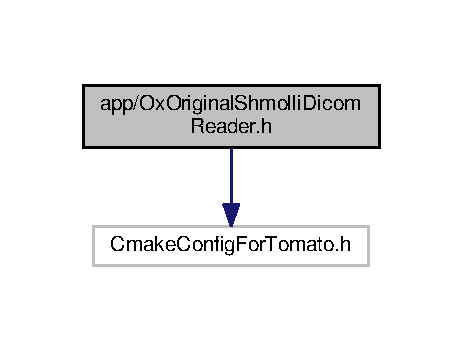
\includegraphics[width=327pt]{_ox_original_shmolli_dicom_reader_8h__incl}
\end{center}
\end{figure}
This graph shows which files directly or indirectly include this file\-:
\nopagebreak
\begin{figure}[H]
\begin{center}
\leavevmode
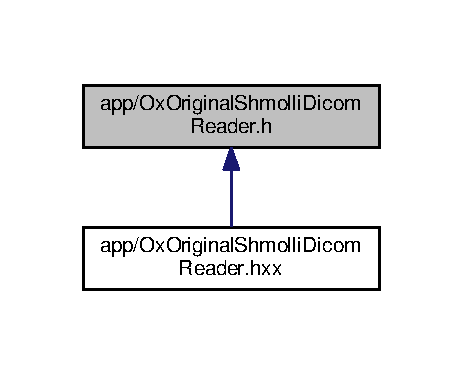
\includegraphics[width=222pt]{_ox_original_shmolli_dicom_reader_8h__dep__incl}
\end{center}
\end{figure}


\subsection{Detailed Description}
\begin{DoxyAuthor}{Author}
Konrad Werys 
\end{DoxyAuthor}
\begin{DoxyDate}{Date}
2018/08/24 
\end{DoxyDate}

\hypertarget{_ox_original_shmolli_dicom_reader_8hxx}{\section{app/\-Ox\-Original\-Shmolli\-Dicom\-Reader.hxx File Reference}
\label{_ox_original_shmolli_dicom_reader_8hxx}\index{app/\-Ox\-Original\-Shmolli\-Dicom\-Reader.\-hxx@{app/\-Ox\-Original\-Shmolli\-Dicom\-Reader.\-hxx}}
}
{\ttfamily \#include $<$itk\-Image\-File\-Reader\-K\-W.\-h$>$}\\*
{\ttfamily \#include \char`\"{}Ox\-Original\-Shmolli\-Dicom\-Reader.\-h\char`\"{}}\\*
Include dependency graph for Ox\-Original\-Shmolli\-Dicom\-Reader.\-hxx\-:
\nopagebreak
\begin{figure}[H]
\begin{center}
\leavevmode
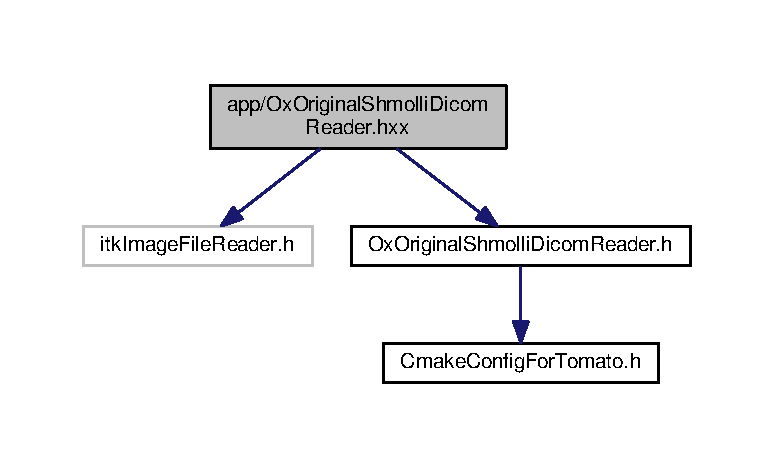
\includegraphics[width=350pt]{_ox_original_shmolli_dicom_reader_8hxx__incl}
\end{center}
\end{figure}


\subsection{Detailed Description}
\begin{DoxyAuthor}{Author}
Konrad Werys 
\end{DoxyAuthor}
\begin{DoxyDate}{Date}
2018/08/24 
\end{DoxyDate}

\hypertarget{_tomato_8h}{\section{app/\-Tomato.h File Reference}
\label{_tomato_8h}\index{app/\-Tomato.\-h@{app/\-Tomato.\-h}}
}
{\ttfamily \#include \char`\"{}Cmake\-Config\-For\-Tomato.\-h\char`\"{}}\\*
{\ttfamily \#include \char`\"{}Tomato\-Options.\-h\char`\"{}}\\*
{\ttfamily \#include \char`\"{}Tomato\-Colormap.\-h\char`\"{}}\\*
{\ttfamily \#include \char`\"{}itk\-Read\-File\-List\-Filter.\-h\char`\"{}}\\*
{\ttfamily \#include \char`\"{}itk\-Sort\-Inv\-Times\-Image\-Filter.\-h\char`\"{}}\\*
{\ttfamily \#include \char`\"{}itk\-Calculator\-T1\-Image\-Filter.\-h\char`\"{}}\\*
{\ttfamily \#include \char`\"{}itk\-Colorbar2\-D\-Image\-Filter.\-h\char`\"{}}\\*
{\ttfamily \#include \char`\"{}itk\-N\-Shmolli\-Samples\-Used\-To123\-Image\-Filter.\-h\char`\"{}}\\*
{\ttfamily \#include \char`\"{}itk\-Time\-Probe.\-h\char`\"{}}\\*
{\ttfamily \#include \char`\"{}gdcm\-U\-I\-D\-Generator.\-h\char`\"{}}\\*
{\ttfamily \#include \char`\"{}itk\-G\-D\-C\-M\-Image\-I\-O.\-h\char`\"{}}\\*
{\ttfamily \#include \char`\"{}itk\-G\-D\-C\-M\-Series\-File\-Names.\-h\char`\"{}}\\*
{\ttfamily \#include \char`\"{}itk\-Multiply\-Image\-Filter.\-h\char`\"{}}\\*
{\ttfamily \#include \char`\"{}itk\-Image\-File\-Writer.\-h\char`\"{}}\\*
{\ttfamily \#include \char`\"{}itk\-File\-Tools.\-h\char`\"{}}\\*
{\ttfamily \#include \char`\"{}itk\-Adapt\-Image\-Filter.\-h\char`\"{}}\\*
{\ttfamily \#include \char`\"{}Tomato.\-hxx\char`\"{}}\\*
{\ttfamily \#include \char`\"{}Tomato\-\_\-export.\-hxx\char`\"{}}\\*
Include dependency graph for Tomato.\-h\-:
\nopagebreak
\begin{figure}[H]
\begin{center}
\leavevmode
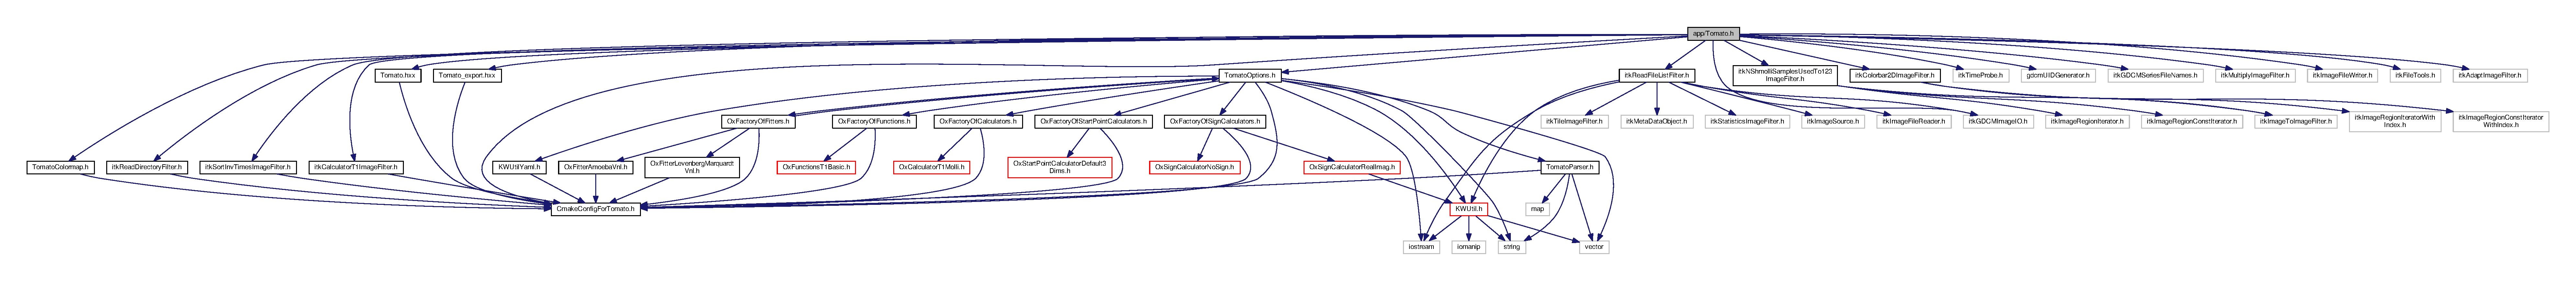
\includegraphics[width=350pt]{_tomato_8h__incl}
\end{center}
\end{figure}
This graph shows which files directly or indirectly include this file\-:
\nopagebreak
\begin{figure}[H]
\begin{center}
\leavevmode
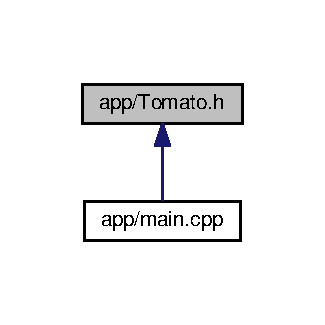
\includegraphics[width=321pt]{_tomato_8h__dep__incl}
\end{center}
\end{figure}


\subsection{Detailed Description}
\begin{DoxyAuthor}{Author}
Konrad Werys 
\end{DoxyAuthor}
\begin{DoxyDate}{Date}
2018/08/14 
\end{DoxyDate}

\hypertarget{_tomato_options_8h}{\section{app/\-Tomato\-Options.h File Reference}
\label{_tomato_options_8h}\index{app/\-Tomato\-Options.\-h@{app/\-Tomato\-Options.\-h}}
}
{\ttfamily \#include $<$iostream$>$}\\*
{\ttfamily \#include $<$vector$>$}\\*
{\ttfamily \#include $<$string$>$}\\*
{\ttfamily \#include \char`\"{}Cmake\-Config\-For\-Tomato.\-h\char`\"{}}\\*
{\ttfamily \#include \char`\"{}Ox\-Factory\-Of\-Calculators.\-h\char`\"{}}\\*
{\ttfamily \#include \char`\"{}Ox\-Factory\-Of\-Fitters.\-h\char`\"{}}\\*
{\ttfamily \#include \char`\"{}Ox\-Factory\-Of\-Functions.\-h\char`\"{}}\\*
{\ttfamily \#include \char`\"{}Ox\-Factory\-Of\-Sign\-Calculators.\-h\char`\"{}}\\*
{\ttfamily \#include \char`\"{}Ox\-Factory\-Of\-Start\-Point\-Calculators.\-h\char`\"{}}\\*
{\ttfamily \#include \char`\"{}Tomato\-Parser.\-h\char`\"{}}\\*
{\ttfamily \#include \char`\"{}K\-W\-Util.\-h\char`\"{}}\\*
{\ttfamily \#include \char`\"{}K\-W\-Util\-Yaml.\-h\char`\"{}}\\*
Include dependency graph for Tomato\-Options.\-h\-:
\nopagebreak
\begin{figure}[H]
\begin{center}
\leavevmode
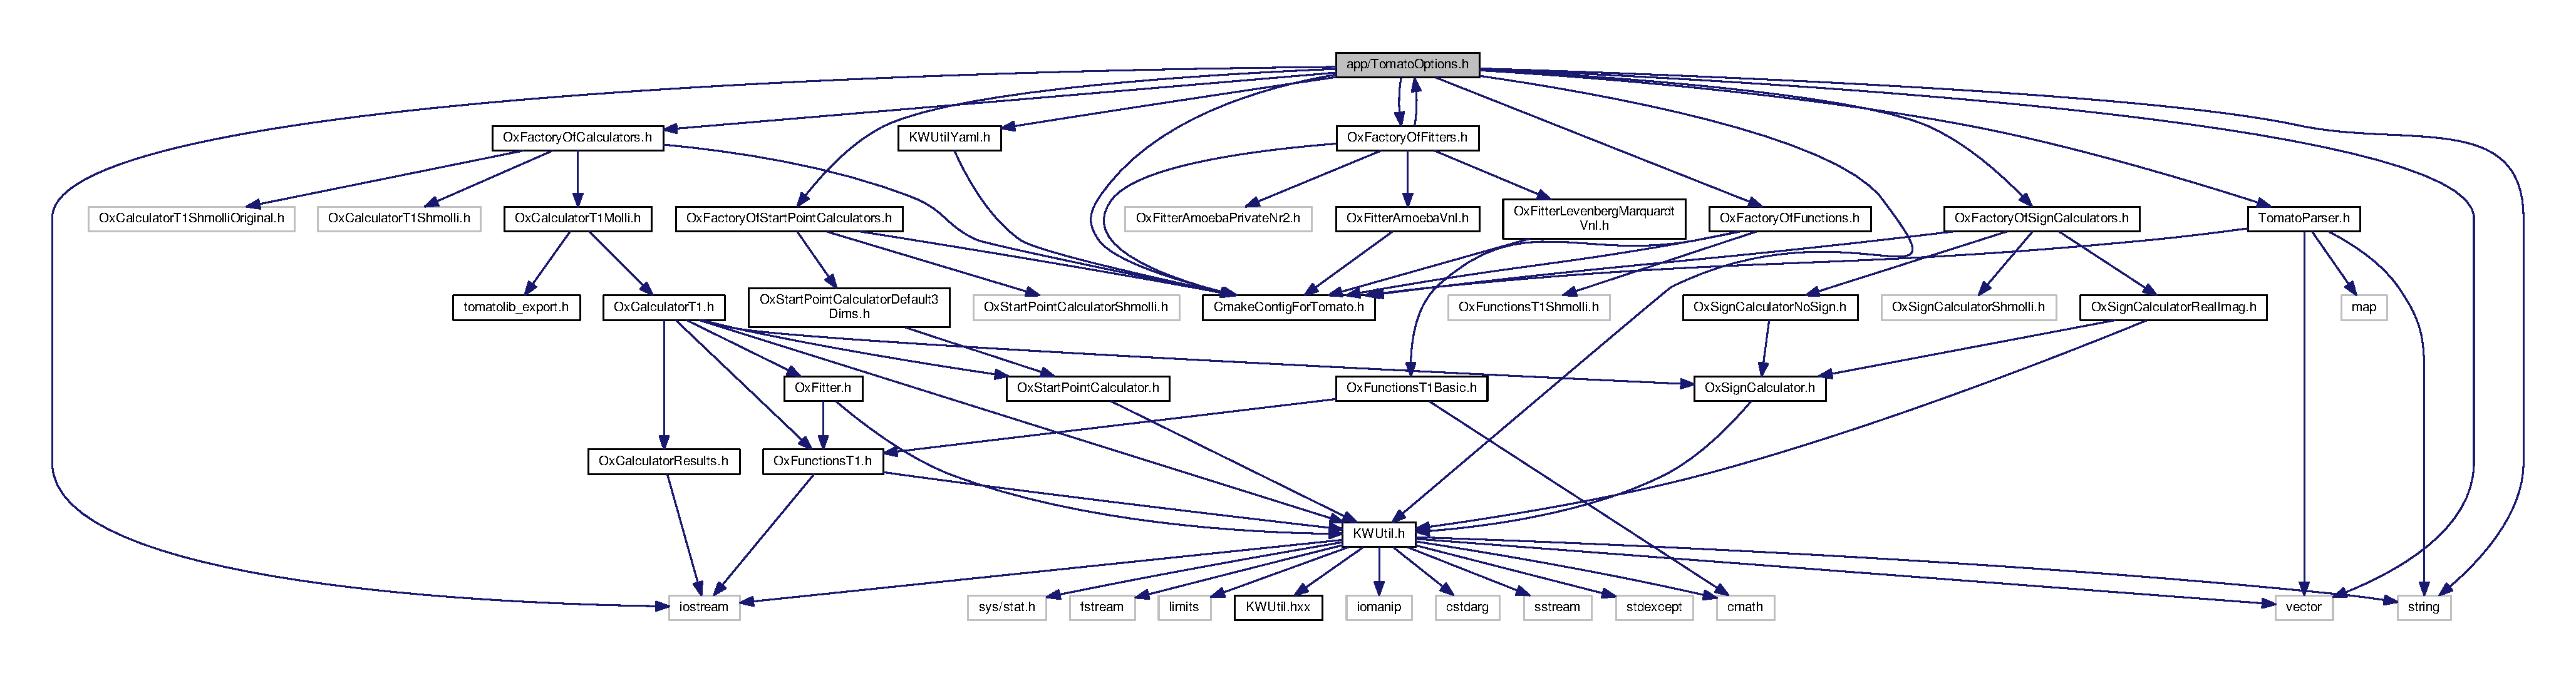
\includegraphics[width=350pt]{_tomato_options_8h__incl}
\end{center}
\end{figure}
This graph shows which files directly or indirectly include this file\-:
\nopagebreak
\begin{figure}[H]
\begin{center}
\leavevmode
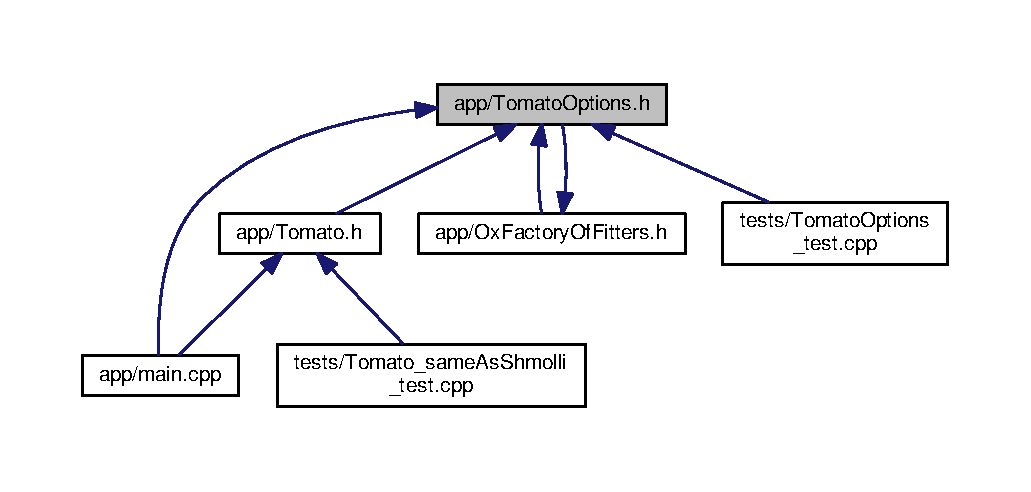
\includegraphics[width=301pt]{_tomato_options_8h__dep__incl}
\end{center}
\end{figure}
\subsection*{Classes}
\begin{DoxyCompactItemize}
\item 
struct \hyperlink{struct_ox_1_1_tomato_options}{Ox\-::\-Tomato\-Options$<$ T\-Y\-P\-E $>$}
\end{DoxyCompactItemize}
\subsection*{Macros}
\begin{DoxyCompactItemize}
\item 
\hypertarget{_tomato_options_8h_aa409ed425e3d493c4e1dcd695f6011df}{\#define {\bfseries Y\-A\-M\-L\-\_\-\-B\-U\-F\-F\-E\-R\-\_\-\-S\-I\-Z\-E}~65536}\label{_tomato_options_8h_aa409ed425e3d493c4e1dcd695f6011df}

\end{DoxyCompactItemize}


\subsection{Detailed Description}
\begin{DoxyAuthor}{Author}
Konrad Werys 
\end{DoxyAuthor}
\begin{DoxyDate}{Date}
2018/08/18 
\end{DoxyDate}

\hypertarget{itk_calculator_t1_image_filter_8h}{\section{lib/itk\-Calculator\-T1\-Image\-Filter.h File Reference}
\label{itk_calculator_t1_image_filter_8h}\index{lib/itk\-Calculator\-T1\-Image\-Filter.\-h@{lib/itk\-Calculator\-T1\-Image\-Filter.\-h}}
}
{\ttfamily \#include \char`\"{}Cmake\-Config\-For\-Ox\-Shmolli2.\-h\char`\"{}}\\*
Include dependency graph for itk\-Calculator\-T1\-Image\-Filter.\-h\-:
\nopagebreak
\begin{figure}[H]
\begin{center}
\leavevmode
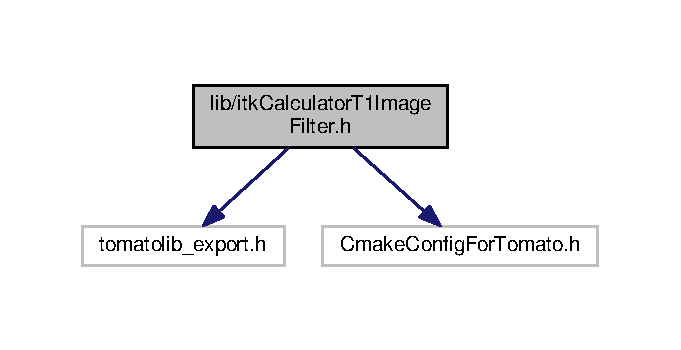
\includegraphics[width=228pt]{itk_calculator_t1_image_filter_8h__incl}
\end{center}
\end{figure}
This graph shows which files directly or indirectly include this file\-:
\nopagebreak
\begin{figure}[H]
\begin{center}
\leavevmode
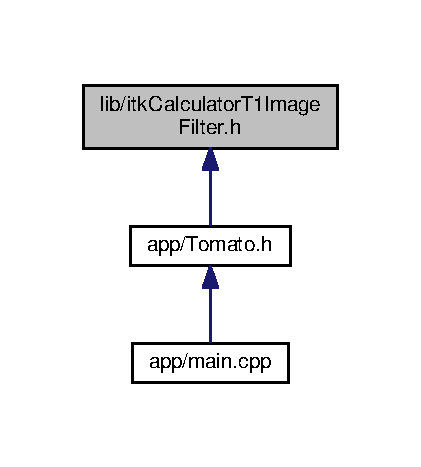
\includegraphics[width=202pt]{itk_calculator_t1_image_filter_8h__dep__incl}
\end{center}
\end{figure}


\subsection{Detailed Description}
\begin{DoxyAuthor}{Author}
Konrad Werys 
\end{DoxyAuthor}
\begin{DoxyDate}{Date}
2018/08/13 
\end{DoxyDate}

\hypertarget{itk_calculator_t1_image_filter_8hxx}{}\section{lib/itk\+Calculator\+T1\+Image\+Filter.hxx File Reference}
\label{itk_calculator_t1_image_filter_8hxx}\index{lib/itk\+Calculator\+T1\+Image\+Filter.\+hxx@{lib/itk\+Calculator\+T1\+Image\+Filter.\+hxx}}
{\ttfamily \#include \char`\"{}Cmake\+Config\+For\+Tomato.\+h\char`\"{}}\\*
Include dependency graph for itk\+Calculator\+T1\+Image\+Filter.\+hxx\+:
\nopagebreak
\begin{figure}[H]
\begin{center}
\leavevmode
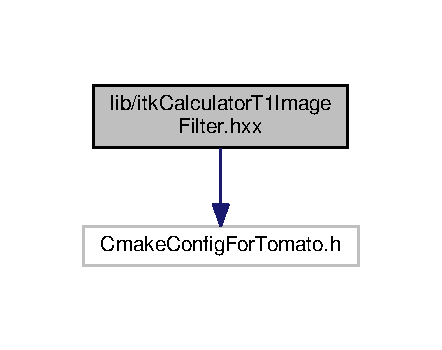
\includegraphics[width=212pt]{itk_calculator_t1_image_filter_8hxx__incl}
\end{center}
\end{figure}


\subsection{Detailed Description}
\begin{DoxyAuthor}{Author}
Konrad Werys 
\end{DoxyAuthor}
\begin{DoxyDate}{Date}
2018/08/13 
\end{DoxyDate}

\hypertarget{_k_w_util_yaml_8h}{\section{lib/\-K\-W\-Util\-Yaml.h File Reference}
\label{_k_w_util_yaml_8h}\index{lib/\-K\-W\-Util\-Yaml.\-h@{lib/\-K\-W\-Util\-Yaml.\-h}}
}
This graph shows which files directly or indirectly include this file\-:
\nopagebreak
\begin{figure}[H]
\begin{center}
\leavevmode
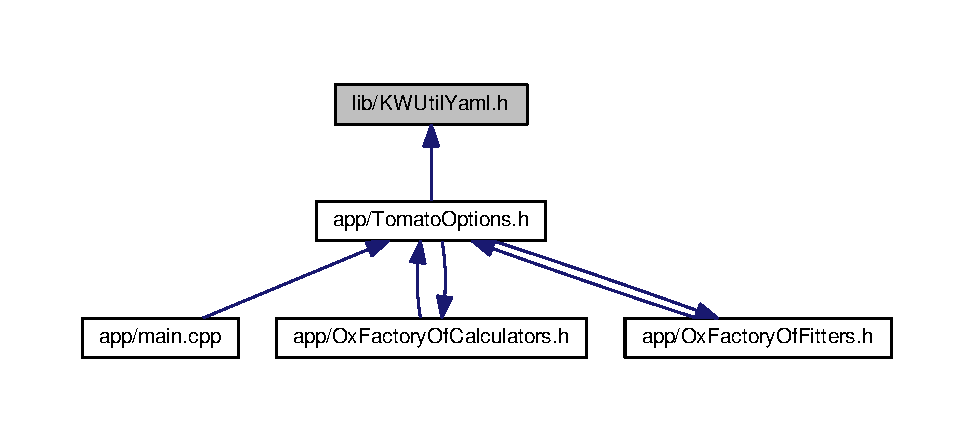
\includegraphics[width=350pt]{_k_w_util_yaml_8h__dep__incl}
\end{center}
\end{figure}
\subsection*{Classes}
\begin{DoxyCompactItemize}
\item 
class \hyperlink{class_k_w_util_yaml}{K\-W\-Util\-Yaml}
\end{DoxyCompactItemize}


\subsection{Detailed Description}
\begin{DoxyAuthor}{Author}
Konrad Werys 
\end{DoxyAuthor}
\begin{DoxyDate}{Date}
2018/11/16 
\end{DoxyDate}

\hypertarget{_ox_calculator_t1_molli_8h}{\section{lib/\-Ox\-Calculator\-T1\-Molli.h File Reference}
\label{_ox_calculator_t1_molli_8h}\index{lib/\-Ox\-Calculator\-T1\-Molli.\-h@{lib/\-Ox\-Calculator\-T1\-Molli.\-h}}
}
{\ttfamily \#include \char`\"{}Ox\-Calculator\-T1.\-h\char`\"{}}\\*
Include dependency graph for Ox\-Calculator\-T1\-Molli.\-h\-:
\nopagebreak
\begin{figure}[H]
\begin{center}
\leavevmode
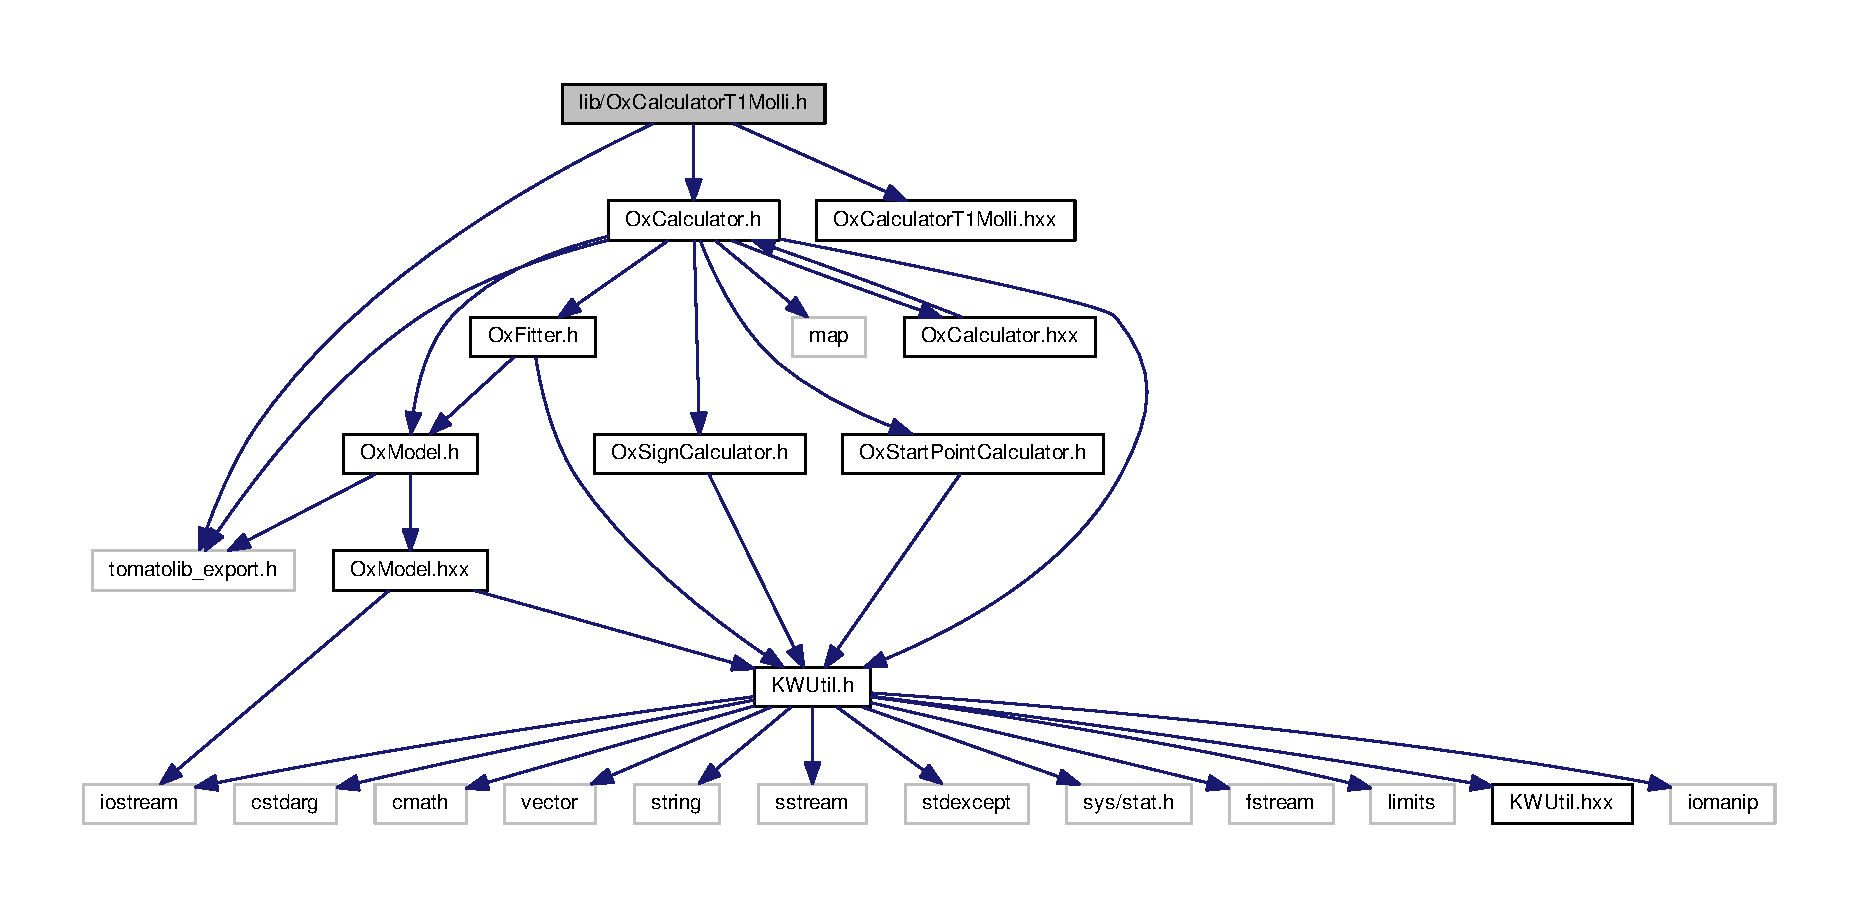
\includegraphics[width=350pt]{_ox_calculator_t1_molli_8h__incl}
\end{center}
\end{figure}
This graph shows which files directly or indirectly include this file\-:
\nopagebreak
\begin{figure}[H]
\begin{center}
\leavevmode
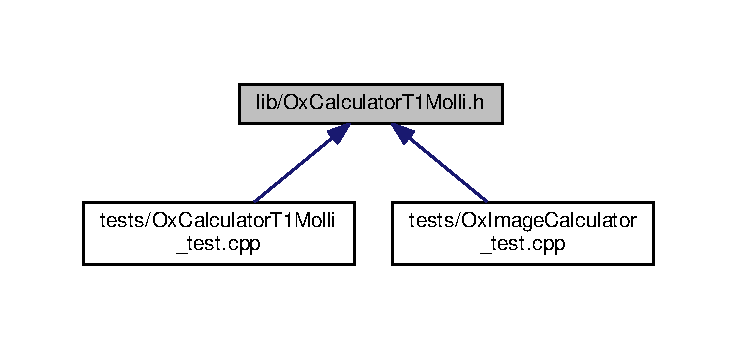
\includegraphics[width=210pt]{_ox_calculator_t1_molli_8h__dep__incl}
\end{center}
\end{figure}
\subsection*{Classes}
\begin{DoxyCompactItemize}
\item 
class \hyperlink{class_ox_1_1_calculator_t1_molli}{Ox\-::\-Calculator\-T1\-Molli$<$ Measure\-Type $>$}
\end{DoxyCompactItemize}


\subsection{Detailed Description}
\begin{DoxyAuthor}{Author}
Konrad Werys 
\end{DoxyAuthor}
\begin{DoxyDate}{Date}
2018/08/01 
\end{DoxyDate}

\hypertarget{_ox_calculator_t1_molli_8hxx}{\section{lib/\-Ox\-Calculator\-T1\-Molli.hxx File Reference}
\label{_ox_calculator_t1_molli_8hxx}\index{lib/\-Ox\-Calculator\-T1\-Molli.\-hxx@{lib/\-Ox\-Calculator\-T1\-Molli.\-hxx}}
}
This graph shows which files directly or indirectly include this file\-:
\nopagebreak
\begin{figure}[H]
\begin{center}
\leavevmode
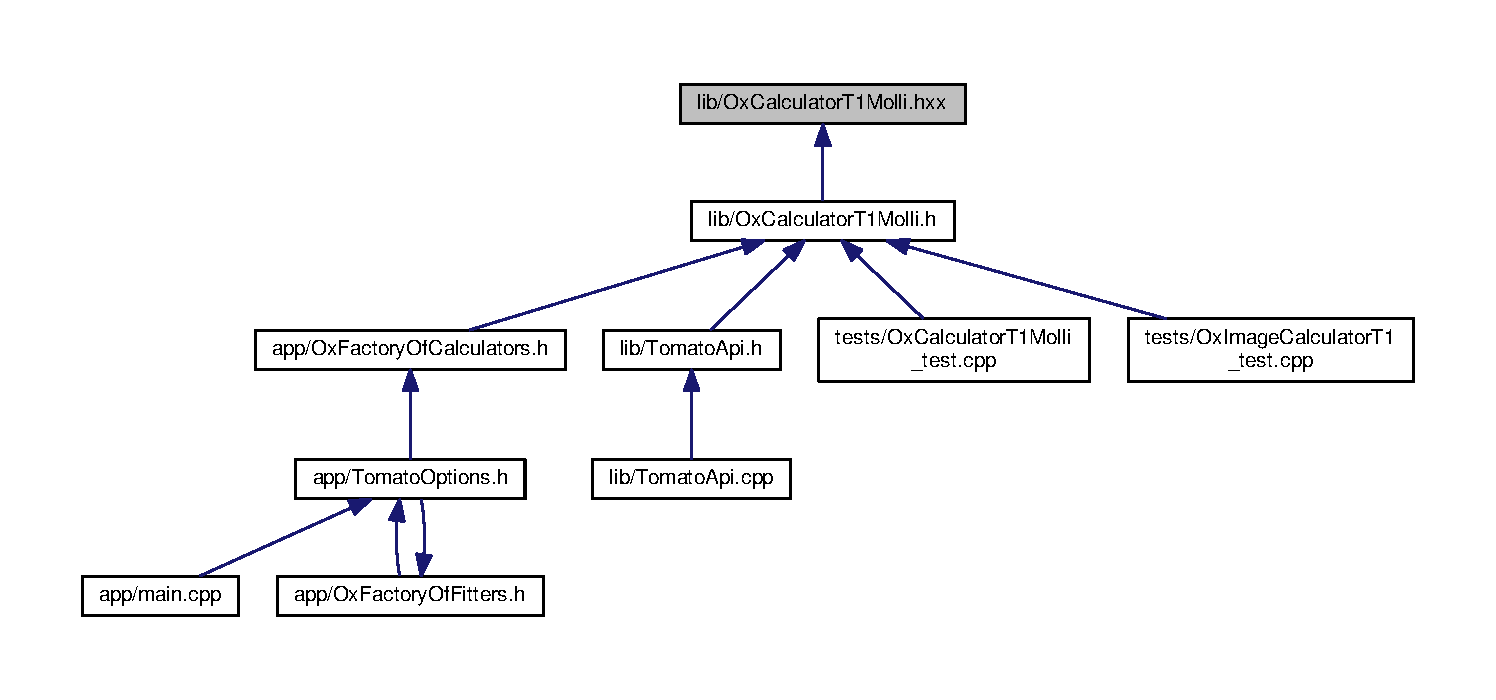
\includegraphics[width=350pt]{_ox_calculator_t1_molli_8hxx__dep__incl}
\end{center}
\end{figure}


\subsection{Detailed Description}
\begin{DoxyAuthor}{Author}
Konrad Werys 
\end{DoxyAuthor}
\begin{DoxyDate}{Date}
2019/01/15 
\end{DoxyDate}

\hypertarget{_ox_fitter_8h}{\section{lib/\-Ox\-Fitter.h File Reference}
\label{_ox_fitter_8h}\index{lib/\-Ox\-Fitter.\-h@{lib/\-Ox\-Fitter.\-h}}
}
{\ttfamily \#include \char`\"{}Ox\-Functions\-T1.\-h\char`\"{}}\\*
{\ttfamily \#include \char`\"{}K\-W\-Util.\-h\char`\"{}}\\*
Include dependency graph for Ox\-Fitter.\-h\-:
\nopagebreak
\begin{figure}[H]
\begin{center}
\leavevmode
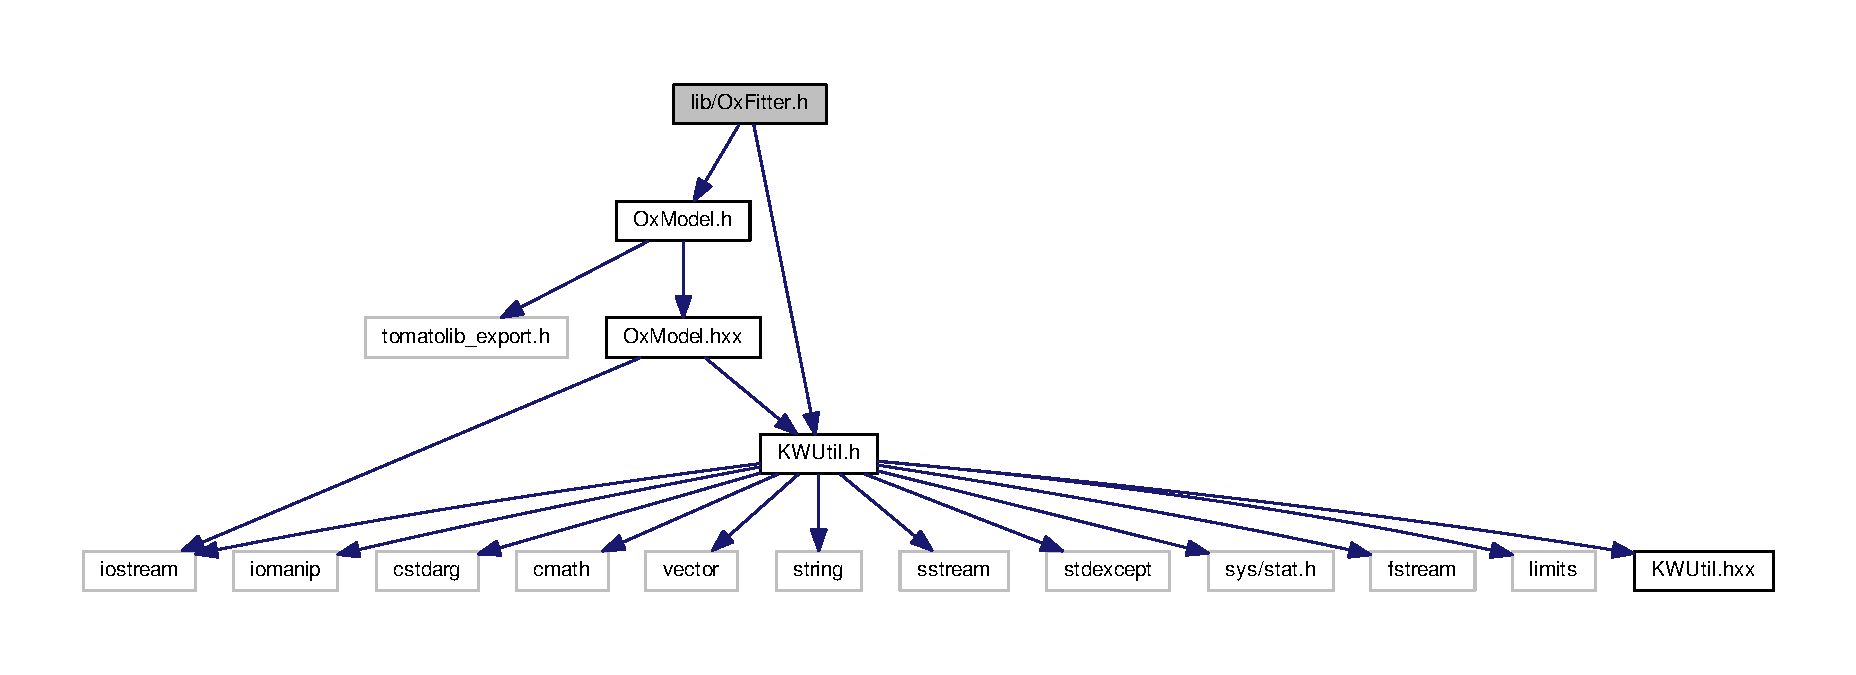
\includegraphics[width=350pt]{_ox_fitter_8h__incl}
\end{center}
\end{figure}
This graph shows which files directly or indirectly include this file\-:
\nopagebreak
\begin{figure}[H]
\begin{center}
\leavevmode
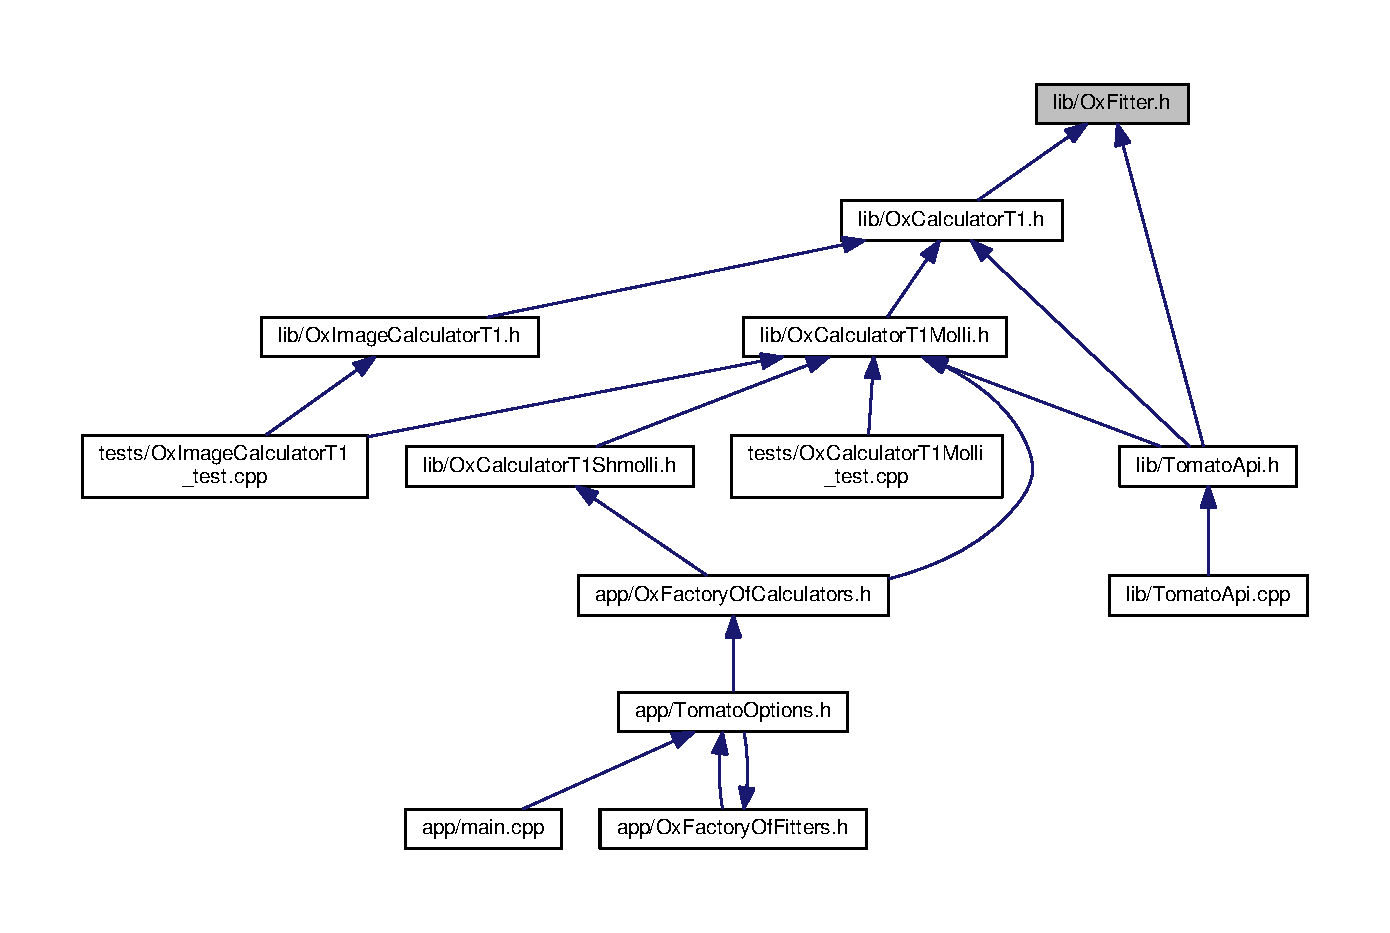
\includegraphics[width=350pt]{_ox_fitter_8h__dep__incl}
\end{center}
\end{figure}
\subsection*{Classes}
\begin{DoxyCompactItemize}
\item 
class \hyperlink{class_ox_1_1_fitter}{Ox\-::\-Fitter$<$ Measure\-Type $>$}
\end{DoxyCompactItemize}


\subsection{Detailed Description}
\begin{DoxyAuthor}{Author}
Konrad Werys 
\end{DoxyAuthor}
\begin{DoxyDate}{Date}
2018/07/29 
\end{DoxyDate}

\hypertarget{_ox_fitter_amoeba_nr2_8h}{\section{lib/\-Ox\-Fitter\-Amoeba\-Nr2.h File Reference}
\label{_ox_fitter_amoeba_nr2_8h}\index{lib/\-Ox\-Fitter\-Amoeba\-Nr2.\-h@{lib/\-Ox\-Fitter\-Amoeba\-Nr2.\-h}}
}
{\ttfamily \#include \char`\"{}Cmake\-Config\-For\-Tomato.\-h\char`\"{}}\\*
Include dependency graph for Ox\-Fitter\-Amoeba\-Nr2.\-h\-:
\nopagebreak
\begin{figure}[H]
\begin{center}
\leavevmode
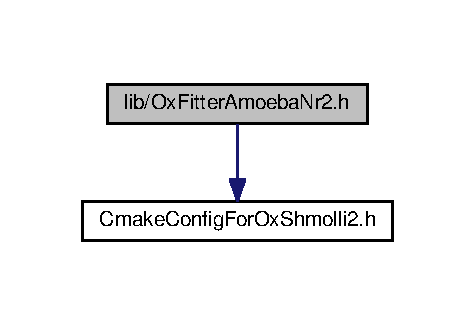
\includegraphics[width=212pt]{_ox_fitter_amoeba_nr2_8h__incl}
\end{center}
\end{figure}


\subsection{Detailed Description}
\begin{DoxyAuthor}{Author}
Konrad Werys 
\end{DoxyAuthor}
\begin{DoxyDate}{Date}
2018/08/06 
\end{DoxyDate}

\hypertarget{_ox_fitter_amoeba_vnl_8h}{\section{lib/\-Ox\-Fitter\-Amoeba\-Vnl.h File Reference}
\label{_ox_fitter_amoeba_vnl_8h}\index{lib/\-Ox\-Fitter\-Amoeba\-Vnl.\-h@{lib/\-Ox\-Fitter\-Amoeba\-Vnl.\-h}}
}
{\ttfamily \#include \char`\"{}Cmake\-Config\-For\-Tomato.\-h\char`\"{}}\\*
Include dependency graph for Ox\-Fitter\-Amoeba\-Vnl.\-h\-:
\nopagebreak
\begin{figure}[H]
\begin{center}
\leavevmode
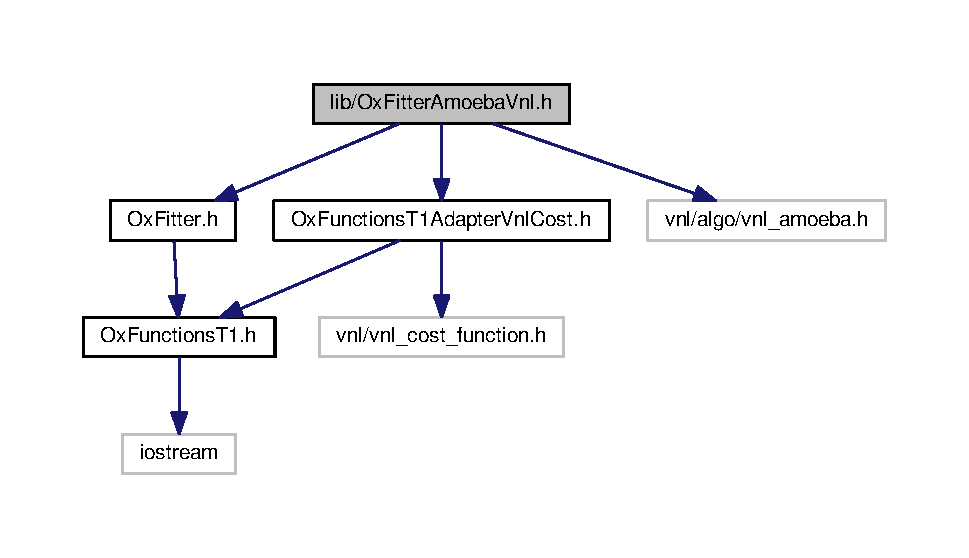
\includegraphics[width=212pt]{_ox_fitter_amoeba_vnl_8h__incl}
\end{center}
\end{figure}
This graph shows which files directly or indirectly include this file\-:
\nopagebreak
\begin{figure}[H]
\begin{center}
\leavevmode
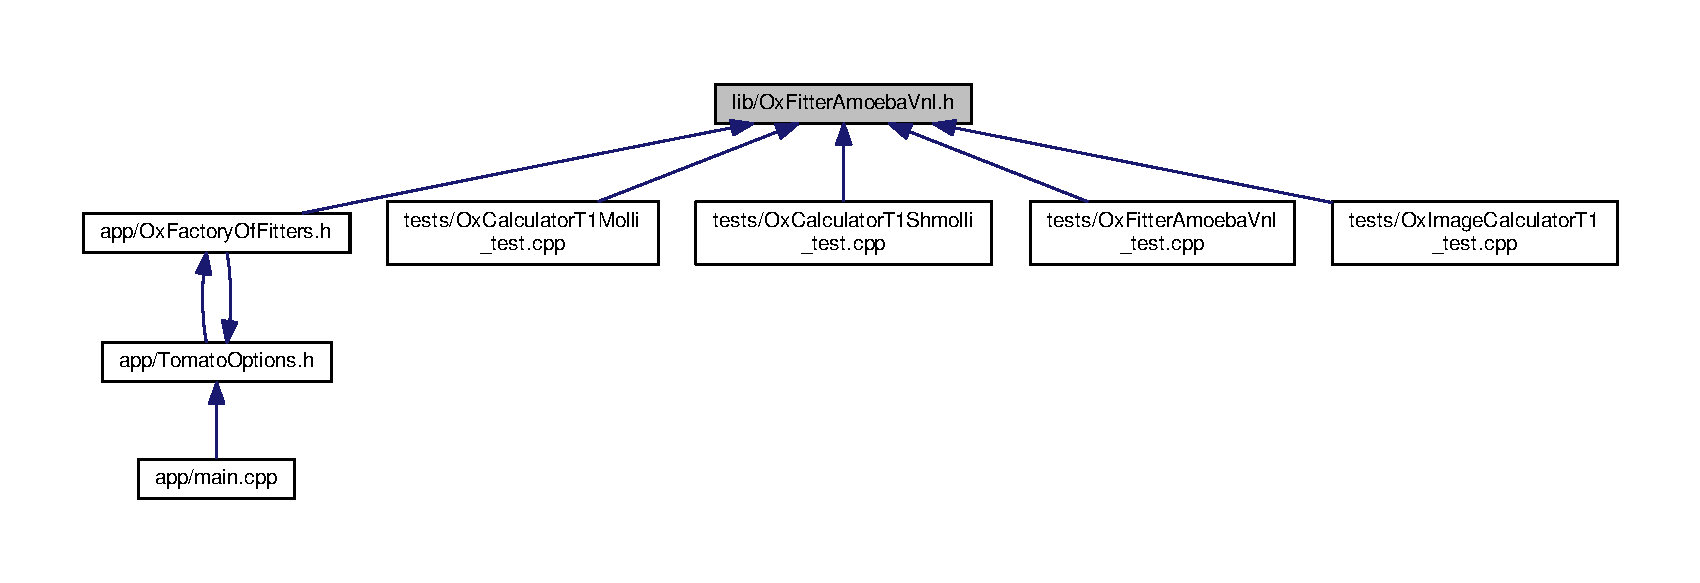
\includegraphics[width=350pt]{_ox_fitter_amoeba_vnl_8h__dep__incl}
\end{center}
\end{figure}


\subsection{Detailed Description}
\begin{DoxyAuthor}{Author}
Konrad Werys 
\end{DoxyAuthor}
\begin{DoxyDate}{Date}
2018/07/30 
\end{DoxyDate}

\hypertarget{_ox_fitter_levenberg_marquardt_vnl_8h}{\section{lib/\-Ox\-Fitter\-Levenberg\-Marquardt\-Vnl.h File Reference}
\label{_ox_fitter_levenberg_marquardt_vnl_8h}\index{lib/\-Ox\-Fitter\-Levenberg\-Marquardt\-Vnl.\-h@{lib/\-Ox\-Fitter\-Levenberg\-Marquardt\-Vnl.\-h}}
}
{\ttfamily \#include \char`\"{}Ox\-Fitter.\-h\char`\"{}}\\*
{\ttfamily \#include \char`\"{}Ox\-Functions\-T1\-Adapter\-Vnl\-Least\-Squares.\-h\char`\"{}}\\*
{\ttfamily \#include $<$vnl/algo/vnl\-\_\-levenberg\-\_\-marquardt.\-h$>$}\\*
Include dependency graph for Ox\-Fitter\-Levenberg\-Marquardt\-Vnl.\-h\-:
\nopagebreak
\begin{figure}[H]
\begin{center}
\leavevmode
\includegraphics[width=350pt]{_ox_fitter_levenberg_marquardt_vnl_8h__incl}
\end{center}
\end{figure}
This graph shows which files directly or indirectly include this file\-:
\nopagebreak
\begin{figure}[H]
\begin{center}
\leavevmode
\includegraphics[width=350pt]{_ox_fitter_levenberg_marquardt_vnl_8h__dep__incl}
\end{center}
\end{figure}
\subsection*{Classes}
\begin{DoxyCompactItemize}
\item 
class \hyperlink{class_ox_1_1_fitter_levenberg_marquardt_vnl}{Ox\-::\-Fitter\-Levenberg\-Marquardt\-Vnl$<$ Measure\-Type $>$}
\end{DoxyCompactItemize}


\subsection{Detailed Description}
\begin{DoxyAuthor}{Author}
Konrad Werys 
\end{DoxyAuthor}
\begin{DoxyDate}{Date}
2018/07/31 
\end{DoxyDate}

\hypertarget{_ox_functions_t1_8h}{}\section{lib/\+Ox\+Functions\+T1.h File Reference}
\label{_ox_functions_t1_8h}\index{lib/\+Ox\+Functions\+T1.\+h@{lib/\+Ox\+Functions\+T1.\+h}}
This graph shows which files directly or indirectly include this file\+:
% FIG 0
\subsection*{Classes}
\begin{DoxyCompactItemize}
\item 
class \mbox{\hyperlink{class_ox_1_1_functions_t1}{Ox\+::\+Functions\+T1$<$ Measure\+Type $>$}}
\begin{DoxyCompactList}\small\item\em Container for a model function, cost function and Least-\/\+Squares function. And derivatives. \end{DoxyCompactList}\end{DoxyCompactItemize}


\subsection{Detailed Description}
\begin{DoxyAuthor}{Author}
Konrad Werys 
\end{DoxyAuthor}
\begin{DoxyDate}{Date}
2018/08/29 
\end{DoxyDate}

\hypertarget{_ox_functions_t1_adapter_vnl_cost_8h}{\section{lib/\-Ox\-Functions\-T1\-Adapter\-Vnl\-Cost.h File Reference}
\label{_ox_functions_t1_adapter_vnl_cost_8h}\index{lib/\-Ox\-Functions\-T1\-Adapter\-Vnl\-Cost.\-h@{lib/\-Ox\-Functions\-T1\-Adapter\-Vnl\-Cost.\-h}}
}
{\ttfamily \#include $<$vnl/vnl\-\_\-cost\-\_\-function.\-h$>$}\\*
{\ttfamily \#include \char`\"{}Ox\-Functions\-T1.\-h\char`\"{}}\\*
Include dependency graph for Ox\-Functions\-T1\-Adapter\-Vnl\-Cost.\-h\-:
\nopagebreak
\begin{figure}[H]
\begin{center}
\leavevmode
\includegraphics[width=350pt]{_ox_functions_t1_adapter_vnl_cost_8h__incl}
\end{center}
\end{figure}
This graph shows which files directly or indirectly include this file\-:
\nopagebreak
\begin{figure}[H]
\begin{center}
\leavevmode
\includegraphics[width=350pt]{_ox_functions_t1_adapter_vnl_cost_8h__dep__incl}
\end{center}
\end{figure}
\subsection*{Classes}
\begin{DoxyCompactItemize}
\item 
class \hyperlink{class_ox_1_1_functions_t1_adapter_vnl_cost}{Ox\-::\-Functions\-T1\-Adapter\-Vnl\-Cost}
\end{DoxyCompactItemize}


\subsection{Detailed Description}
\begin{DoxyAuthor}{Author}
Konrad Werys 
\end{DoxyAuthor}
\begin{DoxyDate}{Date}
2018/07/30 
\end{DoxyDate}

\hypertarget{_ox_functions_t1_adapter_vnl_least_squares_8h}{\section{lib/\-Ox\-Functions\-T1\-Adapter\-Vnl\-Least\-Squares.h File Reference}
\label{_ox_functions_t1_adapter_vnl_least_squares_8h}\index{lib/\-Ox\-Functions\-T1\-Adapter\-Vnl\-Least\-Squares.\-h@{lib/\-Ox\-Functions\-T1\-Adapter\-Vnl\-Least\-Squares.\-h}}
}
{\ttfamily \#include \char`\"{}Cmake\-Config\-For\-Tomato.\-h\char`\"{}}\\*
Include dependency graph for Ox\-Functions\-T1\-Adapter\-Vnl\-Least\-Squares.\-h\-:
\nopagebreak
\begin{figure}[H]
\begin{center}
\leavevmode
\includegraphics[width=212pt]{_ox_functions_t1_adapter_vnl_least_squares_8h__incl}
\end{center}
\end{figure}
This graph shows which files directly or indirectly include this file\-:
\nopagebreak
\begin{figure}[H]
\begin{center}
\leavevmode
\includegraphics[width=222pt]{_ox_functions_t1_adapter_vnl_least_squares_8h__dep__incl}
\end{center}
\end{figure}


\subsection{Detailed Description}
\begin{DoxyAuthor}{Author}
Konrad Werys 
\end{DoxyAuthor}
\begin{DoxyDate}{Date}
2018/07/30 
\end{DoxyDate}

\hypertarget{_ox_functions_t1_basic_8h}{\section{lib/\-Ox\-Functions\-T1\-Basic.h File Reference}
\label{_ox_functions_t1_basic_8h}\index{lib/\-Ox\-Functions\-T1\-Basic.\-h@{lib/\-Ox\-Functions\-T1\-Basic.\-h}}
}
{\ttfamily \#include \char`\"{}Ox\-Functions\-T1.\-h\char`\"{}}\\*
{\ttfamily \#include $<$cmath$>$}\\*
{\ttfamily \#include \char`\"{}Ox\-Functions\-T1\-Basic.\-hxx\char`\"{}}\\*
Include dependency graph for Ox\-Functions\-T1\-Basic.\-h\-:
\nopagebreak
\begin{figure}[H]
\begin{center}
\leavevmode
\includegraphics[width=350pt]{_ox_functions_t1_basic_8h__incl}
\end{center}
\end{figure}
This graph shows which files directly or indirectly include this file\-:
\nopagebreak
\begin{figure}[H]
\begin{center}
\leavevmode
\includegraphics[width=350pt]{_ox_functions_t1_basic_8h__dep__incl}
\end{center}
\end{figure}
\subsection*{Classes}
\begin{DoxyCompactItemize}
\item 
class \hyperlink{class_ox_1_1_functions_t1_basic}{Ox\-::\-Functions\-T1\-Basic$<$ Measure\-Type $>$}
\begin{DoxyCompactList}\small\item\em Container for a basic model function $\sqrt{A-B\exp(t/T_1^*)}$, cost function and Least-\/\-Squares function and derivatives. \end{DoxyCompactList}\end{DoxyCompactItemize}


\subsection{Detailed Description}
\begin{DoxyAuthor}{Author}
Konrad Werys 
\end{DoxyAuthor}
\begin{DoxyDate}{Date}
2018/07/29 
\end{DoxyDate}

\hypertarget{_ox_functions_t1_basic_8hxx}{}\section{lib/\+Ox\+Functions\+T1\+Basic.hxx File Reference}
\label{_ox_functions_t1_basic_8hxx}\index{lib/\+Ox\+Functions\+T1\+Basic.\+hxx@{lib/\+Ox\+Functions\+T1\+Basic.\+hxx}}
This graph shows which files directly or indirectly include this file\+:
% FIG 0


\subsection{Detailed Description}
\begin{DoxyAuthor}{Author}
Konrad Werys 
\end{DoxyAuthor}
\begin{DoxyDate}{Date}
2018/08/29 
\end{DoxyDate}

\hypertarget{_ox_sign_calculator_8h}{}\section{lib/\+Ox\+Sign\+Calculator.h File Reference}
\label{_ox_sign_calculator_8h}\index{lib/\+Ox\+Sign\+Calculator.\+h@{lib/\+Ox\+Sign\+Calculator.\+h}}
This graph shows which files directly or indirectly include this file\+:
% FIG 0
\subsection*{Classes}
\begin{DoxyCompactItemize}
\item 
class \mbox{\hyperlink{class_ox_1_1_sign_calculator}{Ox\+::\+Sign\+Calculator$<$ Measure\+Type $>$}}
\end{DoxyCompactItemize}


\subsection{Detailed Description}
\begin{DoxyAuthor}{Author}
Konrad Werys 
\end{DoxyAuthor}
\begin{DoxyDate}{Date}
2018/08/29 
\end{DoxyDate}

\hypertarget{_ox_sign_calculator_no_sign_8h}{}\section{lib/\+Ox\+Sign\+Calculator\+No\+Sign.h File Reference}
\label{_ox_sign_calculator_no_sign_8h}\index{lib/\+Ox\+Sign\+Calculator\+No\+Sign.\+h@{lib/\+Ox\+Sign\+Calculator\+No\+Sign.\+h}}
{\ttfamily \#include \char`\"{}Ox\+Sign\+Calculator.\+h\char`\"{}}\\*
Include dependency graph for Ox\+Sign\+Calculator\+No\+Sign.\+h\+:
\nopagebreak
\begin{figure}[H]
\begin{center}
\leavevmode
\includegraphics[width=350pt]{_ox_sign_calculator_no_sign_8h__incl}
\end{center}
\end{figure}
This graph shows which files directly or indirectly include this file\+:
\nopagebreak
\begin{figure}[H]
\begin{center}
\leavevmode
\includegraphics[width=350pt]{_ox_sign_calculator_no_sign_8h__dep__incl}
\end{center}
\end{figure}
\subsection*{Classes}
\begin{DoxyCompactItemize}
\item 
class \hyperlink{class_ox_1_1_sign_calculator_no_sign}{Ox\+::\+Sign\+Calculator\+No\+Sign$<$ Measure\+Type $>$}
\end{DoxyCompactItemize}


\subsection{Detailed Description}
\begin{DoxyAuthor}{Author}
Konrad Werys 
\end{DoxyAuthor}
\begin{DoxyDate}{Date}
2018/08/13 
\end{DoxyDate}

\hypertarget{_ox_sign_calculator_real_imag_8h}{\section{lib/\-Ox\-Sign\-Calculator\-Real\-Imag.h File Reference}
\label{_ox_sign_calculator_real_imag_8h}\index{lib/\-Ox\-Sign\-Calculator\-Real\-Imag.\-h@{lib/\-Ox\-Sign\-Calculator\-Real\-Imag.\-h}}
}
{\ttfamily \#include \char`\"{}Ox\-Sign\-Calculator.\-h\char`\"{}}\\*
{\ttfamily \#include \char`\"{}K\-W\-Util.\-h\char`\"{}}\\*
Include dependency graph for Ox\-Sign\-Calculator\-Real\-Imag.\-h\-:
\nopagebreak
\begin{figure}[H]
\begin{center}
\leavevmode
\includegraphics[width=350pt]{_ox_sign_calculator_real_imag_8h__incl}
\end{center}
\end{figure}
This graph shows which files directly or indirectly include this file\-:
\nopagebreak
\begin{figure}[H]
\begin{center}
\leavevmode
\includegraphics[width=350pt]{_ox_sign_calculator_real_imag_8h__dep__incl}
\end{center}
\end{figure}
\subsection*{Classes}
\begin{DoxyCompactItemize}
\item 
class \hyperlink{class_ox_1_1_sign_calculator_real_imag}{Ox\-::\-Sign\-Calculator\-Real\-Imag$<$ Measure\-Type $>$}
\end{DoxyCompactItemize}


\subsection{Detailed Description}
\begin{DoxyAuthor}{Author}
Konrad Werys 
\end{DoxyAuthor}
\begin{DoxyDate}{Date}
2018/08/01 
\end{DoxyDate}

\hypertarget{_ox_start_point_calculator_8h}{\section{lib/\-Ox\-Start\-Point\-Calculator.h File Reference}
\label{_ox_start_point_calculator_8h}\index{lib/\-Ox\-Start\-Point\-Calculator.\-h@{lib/\-Ox\-Start\-Point\-Calculator.\-h}}
}
This graph shows which files directly or indirectly include this file\-:
\nopagebreak
\begin{figure}[H]
\begin{center}
\leavevmode
\includegraphics[width=218pt]{_ox_start_point_calculator_8h__dep__incl}
\end{center}
\end{figure}
\subsection*{Classes}
\begin{DoxyCompactItemize}
\item 
class \hyperlink{class_ox_1_1_start_point_calculator}{Ox\-::\-Start\-Point\-Calculator$<$ Measure\-Type $>$}
\end{DoxyCompactItemize}


\subsection{Detailed Description}
\begin{DoxyAuthor}{Author}
Konrad Werys 
\end{DoxyAuthor}
\begin{DoxyDate}{Date}
2018/07/29 
\end{DoxyDate}

\hypertarget{_ox_start_point_calculator_default3_dims_8h}{\section{lib/\-Ox\-Start\-Point\-Calculator\-Default3\-Dims.h File Reference}
\label{_ox_start_point_calculator_default3_dims_8h}\index{lib/\-Ox\-Start\-Point\-Calculator\-Default3\-Dims.\-h@{lib/\-Ox\-Start\-Point\-Calculator\-Default3\-Dims.\-h}}
}
{\ttfamily \#include \char`\"{}Ox\-Start\-Point\-Calculator.\-h\char`\"{}}\\*
Include dependency graph for Ox\-Start\-Point\-Calculator\-Default3\-Dims.\-h\-:
\nopagebreak
\begin{figure}[H]
\begin{center}
\leavevmode
\includegraphics[width=350pt]{_ox_start_point_calculator_default3_dims_8h__incl}
\end{center}
\end{figure}
This graph shows which files directly or indirectly include this file\-:
\nopagebreak
\begin{figure}[H]
\begin{center}
\leavevmode
\includegraphics[width=350pt]{_ox_start_point_calculator_default3_dims_8h__dep__incl}
\end{center}
\end{figure}
\subsection*{Classes}
\begin{DoxyCompactItemize}
\item 
class \hyperlink{class_ox_1_1_start_point_calculator_default3_dims}{Ox\-::\-Start\-Point\-Calculator\-Default3\-Dims$<$ Measure\-Type $>$}
\end{DoxyCompactItemize}


\subsection{Detailed Description}
\begin{DoxyAuthor}{Author}
Konrad Werys 
\end{DoxyAuthor}
\begin{DoxyDate}{Date}
2018/08/10 
\end{DoxyDate}

\hypertarget{_tomato_api_8h}{\section{lib/\-Tomato\-Api.h File Reference}
\label{_tomato_api_8h}\index{lib/\-Tomato\-Api.\-h@{lib/\-Tomato\-Api.\-h}}
}
{\ttfamily \#include \char`\"{}Cmake\-Config\-For\-Tomato.\-h\char`\"{}}\\*
{\ttfamily \#include \char`\"{}tomatolib\-\_\-export.\-h\char`\"{}}\\*
{\ttfamily \#include \char`\"{}Ox\-Calculator.\-h\char`\"{}}\\*
{\ttfamily \#include \char`\"{}Ox\-Calculator\-T1\-Molli.\-h\char`\"{}}\\*
{\ttfamily \#include \char`\"{}Ox\-Fitter.\-h\char`\"{}}\\*
{\ttfamily \#include \char`\"{}Ox\-Model.\-h\char`\"{}}\\*
{\ttfamily \#include \char`\"{}Ox\-Model\-T1\-Three\-Param.\-h\char`\"{}}\\*
{\ttfamily \#include \char`\"{}Ox\-Sign\-Calculator.\-h\char`\"{}}\\*
{\ttfamily \#include \char`\"{}Ox\-Sign\-Calculator\-No\-Sign.\-h\char`\"{}}\\*
{\ttfamily \#include \char`\"{}Ox\-Sign\-Calculator\-Real\-Imag.\-h\char`\"{}}\\*
{\ttfamily \#include \char`\"{}Ox\-Start\-Point\-Calculator\-Basic.\-h\char`\"{}}\\*
Include dependency graph for Tomato\-Api.\-h\-:
\nopagebreak
\begin{figure}[H]
\begin{center}
\leavevmode
\includegraphics[width=350pt]{_tomato_api_8h__incl}
\end{center}
\end{figure}
This graph shows which files directly or indirectly include this file\-:
\nopagebreak
\begin{figure}[H]
\begin{center}
\leavevmode
\includegraphics[width=174pt]{_tomato_api_8h__dep__incl}
\end{center}
\end{figure}
\subsection*{Variables}
\begin{DoxyCompactItemize}
\item 
\hypertarget{namespace_ox_a9b8230abbabcc9e797ae3d9844af1bea}{template class T\-O\-M\-A\-T\-O\-L\-I\-B\-\_\-\-E\-X\-P\-O\-R\-T {\bfseries Ox\-::\-Calculator$<$ double $>$}}\label{namespace_ox_a9b8230abbabcc9e797ae3d9844af1bea}

\item 
\hypertarget{namespace_ox_a7d0473f70666fc11f4c370f408240086}{template class T\-O\-M\-A\-T\-O\-L\-I\-B\-\_\-\-E\-X\-P\-O\-R\-T {\bfseries Ox\-::\-Calculator\-T1\-Molli$<$ double $>$}}\label{namespace_ox_a7d0473f70666fc11f4c370f408240086}

\item 
\hypertarget{namespace_ox_a1e4e4356bc0f519c7b33750ff33594f1}{template class T\-O\-M\-A\-T\-O\-L\-I\-B\-\_\-\-E\-X\-P\-O\-R\-T {\bfseries Ox\-::\-Fitter$<$ double $>$}}\label{namespace_ox_a1e4e4356bc0f519c7b33750ff33594f1}

\item 
\hypertarget{namespace_ox_af85883bfc75370cbe7359ce6f2f8f3b4}{template class T\-O\-M\-A\-T\-O\-L\-I\-B\-\_\-\-E\-X\-P\-O\-R\-T {\bfseries Ox\-::\-Model$<$ double $>$}}\label{namespace_ox_af85883bfc75370cbe7359ce6f2f8f3b4}

\item 
\hypertarget{namespace_ox_adab5d5b6b27e41b97f5a0f721da27773}{template class T\-O\-M\-A\-T\-O\-L\-I\-B\-\_\-\-E\-X\-P\-O\-R\-T {\bfseries Ox\-::\-Model\-T1\-Three\-Param$<$ double $>$}}\label{namespace_ox_adab5d5b6b27e41b97f5a0f721da27773}

\item 
\hypertarget{namespace_ox_aef50802c4cb9bb489316d9b0e764aa81}{template class T\-O\-M\-A\-T\-O\-L\-I\-B\-\_\-\-E\-X\-P\-O\-R\-T {\bfseries Ox\-::\-Sign\-Calculator$<$ double $>$}}\label{namespace_ox_aef50802c4cb9bb489316d9b0e764aa81}

\item 
\hypertarget{namespace_ox_a2e213fe78207181befc0192a210d3adb}{template class T\-O\-M\-A\-T\-O\-L\-I\-B\-\_\-\-E\-X\-P\-O\-R\-T {\bfseries Ox\-::\-Sign\-Calculator\-No\-Sign$<$ double $>$}}\label{namespace_ox_a2e213fe78207181befc0192a210d3adb}

\item 
\hypertarget{namespace_ox_ad5bf210ae8e86f164618f26788b595b1}{template class T\-O\-M\-A\-T\-O\-L\-I\-B\-\_\-\-E\-X\-P\-O\-R\-T {\bfseries Ox\-::\-Sign\-Calculator\-Real\-Imag$<$ double $>$}}\label{namespace_ox_ad5bf210ae8e86f164618f26788b595b1}

\item 
\hypertarget{namespace_ox_a6c87c0e4ce8f92232a88a13445f8cc4e}{template class T\-O\-M\-A\-T\-O\-L\-I\-B\-\_\-\-E\-X\-P\-O\-R\-T {\bfseries Ox\-::\-Start\-Point\-Calculator$<$ double $>$}}\label{namespace_ox_a6c87c0e4ce8f92232a88a13445f8cc4e}

\item 
\hypertarget{namespace_ox_ae34d58307825389c7f280474da9297e3}{template class T\-O\-M\-A\-T\-O\-L\-I\-B\-\_\-\-E\-X\-P\-O\-R\-T {\bfseries Ox\-::\-Start\-Point\-Calculator\-Basic$<$ double $>$}}\label{namespace_ox_ae34d58307825389c7f280474da9297e3}

\end{DoxyCompactItemize}


\subsection{Detailed Description}
\begin{DoxyAuthor}{Author}
Konrad Werys 
\end{DoxyAuthor}
\begin{DoxyDate}{Date}
2019/01/15 This file is necessary to generate Tomato's dynamic library. Consider adding extern to the explicit instantiations For more details refer to \href{http://mrkonrad.github.io/MRKonrad/CMakeDll}{\tt http\-://mrkonrad.\-github.\-io/\-M\-R\-Konrad/\-C\-Make\-Dll} \href{https://github.com/MRKonrad/dllPlayground}{\tt https\-://github.\-com/\-M\-R\-Konrad/dll\-Playground} \href{https://anteru.net/blog/2008/11/19/318/index.html}{\tt https\-://anteru.\-net/blog/2008/11/19/318/index.\-html} 
\end{DoxyDate}

\hypertarget{_tomato_colormap_8cpp}{\section{lib/\-Tomato\-Colormap.cpp File Reference}
\label{_tomato_colormap_8cpp}\index{lib/\-Tomato\-Colormap.\-cpp@{lib/\-Tomato\-Colormap.\-cpp}}
}
{\ttfamily \#include \char`\"{}Tomato\-Colormap.\-h\char`\"{}}\\*
{\ttfamily \#include \char`\"{}gdcm\-Global.\-h\char`\"{}}\\*
{\ttfamily \#include \char`\"{}gdcm\-Base64.\-h\char`\"{}}\\*
Include dependency graph for Tomato\-Colormap.\-cpp\-:
\nopagebreak
\begin{figure}[H]
\begin{center}
\leavevmode
\includegraphics[width=350pt]{_tomato_colormap_8cpp__incl}
\end{center}
\end{figure}


\subsection{Detailed Description}
\begin{DoxyAuthor}{Author}
Konrad Werys 
\end{DoxyAuthor}
\begin{DoxyDate}{Date}
2018/08/24 
\end{DoxyDate}

\hypertarget{_tomato_colormap_8h}{\section{lib/\-Tomato\-Colormap.h File Reference}
\label{_tomato_colormap_8h}\index{lib/\-Tomato\-Colormap.\-h@{lib/\-Tomato\-Colormap.\-h}}
}
{\ttfamily \#include \char`\"{}Cmake\-Config\-For\-Tomato.\-h\char`\"{}}\\*
Include dependency graph for Tomato\-Colormap.\-h\-:
\nopagebreak
\begin{figure}[H]
\begin{center}
\leavevmode
\includegraphics[width=212pt]{_tomato_colormap_8h__incl}
\end{center}
\end{figure}
This graph shows which files directly or indirectly include this file\-:
\nopagebreak
\begin{figure}[H]
\begin{center}
\leavevmode
\includegraphics[width=350pt]{_tomato_colormap_8h__dep__incl}
\end{center}
\end{figure}


\subsection{Detailed Description}
\begin{DoxyAuthor}{Author}
Konrad Werys 
\end{DoxyAuthor}
\begin{DoxyDate}{Date}
2017/08/23 
\end{DoxyDate}

\hypertarget{_tomato_parser_8h}{}\section{lib/\+Tomato\+Parser.h File Reference}
\label{_tomato_parser_8h}\index{lib/\+Tomato\+Parser.\+h@{lib/\+Tomato\+Parser.\+h}}
{\ttfamily \#include \char`\"{}Cmake\+Config\+For\+Tomato.\+h\char`\"{}}\\*
Include dependency graph for Tomato\+Parser.\+h\+:
\nopagebreak
\begin{figure}[H]
\begin{center}
\leavevmode
\includegraphics[width=212pt]{_tomato_parser_8h__incl}
\end{center}
\end{figure}
This graph shows which files directly or indirectly include this file\+:
\nopagebreak
\begin{figure}[H]
\begin{center}
\leavevmode
\includegraphics[width=350pt]{_tomato_parser_8h__dep__incl}
\end{center}
\end{figure}


\subsection{Detailed Description}
\begin{DoxyAuthor}{Author}
Konrad Werys 
\end{DoxyAuthor}
\begin{DoxyDate}{Date}
2018/08/19 
\end{DoxyDate}

\hypertarget{_tomato_parser_8hxx}{}\section{lib/\+Tomato\+Parser.hxx File Reference}
\label{_tomato_parser_8hxx}\index{lib/\+Tomato\+Parser.\+hxx@{lib/\+Tomato\+Parser.\+hxx}}


\subsection{Detailed Description}
\begin{DoxyAuthor}{Author}
Konrad Werys 
\end{DoxyAuthor}
\begin{DoxyDate}{Date}
2018/08/19 
\end{DoxyDate}

\hypertarget{itk_pipeline___calculator_shmolli__test_8cpp}{\section{tests/itk\-Pipeline\-\_\-\-Calculator\-Shmolli\-\_\-test.cpp File Reference}
\label{itk_pipeline___calculator_shmolli__test_8cpp}\index{tests/itk\-Pipeline\-\_\-\-Calculator\-Shmolli\-\_\-test.\-cpp@{tests/itk\-Pipeline\-\_\-\-Calculator\-Shmolli\-\_\-test.\-cpp}}
}
{\ttfamily \#include \char`\"{}Cmake\-Config\-For\-Tomato.\-h\char`\"{}}\\*
Include dependency graph for itk\-Pipeline\-\_\-\-Calculator\-Shmolli\-\_\-test.\-cpp\-:
\nopagebreak
\begin{figure}[H]
\begin{center}
\leavevmode
\includegraphics[width=216pt]{itk_pipeline___calculator_shmolli__test_8cpp__incl}
\end{center}
\end{figure}


\subsection{Detailed Description}
\begin{DoxyAuthor}{Author}
Konrad Werys 
\end{DoxyAuthor}
\begin{DoxyDate}{Date}
2018/10/12 
\end{DoxyDate}

\hypertarget{itk_pipeline__test_8cpp}{\section{tests/itk\-Pipeline\-\_\-test.cpp File Reference}
\label{itk_pipeline__test_8cpp}\index{tests/itk\-Pipeline\-\_\-test.\-cpp@{tests/itk\-Pipeline\-\_\-test.\-cpp}}
}
{\ttfamily \#include \char`\"{}Cmake\-Config\-For\-Ox\-Shmolli2.\-h\char`\"{}}\\*
Include dependency graph for itk\-Pipeline\-\_\-test.\-cpp\-:
\nopagebreak
\begin{figure}[H]
\begin{center}
\leavevmode
\includegraphics[width=228pt]{itk_pipeline__test_8cpp__incl}
\end{center}
\end{figure}


\subsection{Detailed Description}
\begin{DoxyAuthor}{Author}
Konrad Werys 
\end{DoxyAuthor}
\begin{DoxyDate}{Date}
2018/08/14 
\end{DoxyDate}

\hypertarget{itk_sort_inv_times_image_filter__test_8cpp}{\section{tests/itk\-Sort\-Inv\-Times\-Image\-Filter\-\_\-test.cpp File Reference}
\label{itk_sort_inv_times_image_filter__test_8cpp}\index{tests/itk\-Sort\-Inv\-Times\-Image\-Filter\-\_\-test.\-cpp@{tests/itk\-Sort\-Inv\-Times\-Image\-Filter\-\_\-test.\-cpp}}
}
{\ttfamily \#include \char`\"{}Cmake\-Config\-For\-Ox\-Shmolli2.\-h\char`\"{}}\\*
Include dependency graph for itk\-Sort\-Inv\-Times\-Image\-Filter\-\_\-test.\-cpp\-:
\nopagebreak
\begin{figure}[H]
\begin{center}
\leavevmode
\includegraphics[width=228pt]{itk_sort_inv_times_image_filter__test_8cpp__incl}
\end{center}
\end{figure}


\subsection{Detailed Description}
\begin{DoxyAuthor}{Author}
Konrad Werys 
\end{DoxyAuthor}
\begin{DoxyDate}{Date}
2018/08/14 
\end{DoxyDate}

\hypertarget{_k_w_util__test_8cpp}{\section{tests/\-K\-W\-Util\-\_\-test.cpp File Reference}
\label{_k_w_util__test_8cpp}\index{tests/\-K\-W\-Util\-\_\-test.\-cpp@{tests/\-K\-W\-Util\-\_\-test.\-cpp}}
}
{\ttfamily \#include \char`\"{}K\-W\-Util.\-h\char`\"{}}\\*
{\ttfamily \#include \char`\"{}gtest/gtest.\-h\char`\"{}}\\*
Include dependency graph for K\-W\-Util\-\_\-test.\-cpp\-:
\nopagebreak
\begin{figure}[H]
\begin{center}
\leavevmode
\includegraphics[width=350pt]{_k_w_util__test_8cpp__incl}
\end{center}
\end{figure}
\subsection*{Functions}
\begin{DoxyCompactItemize}
\item 
\hypertarget{_k_w_util__test_8cpp_a1c98f2841a55bb84a383720f6c445ece}{{\bfseries T\-E\-S\-T} (\hyperlink{class_k_w_util}{K\-W\-Util}, dicom\-Time2\-Seconds)}\label{_k_w_util__test_8cpp_a1c98f2841a55bb84a383720f6c445ece}

\item 
\hypertarget{_k_w_util__test_8cpp_a7e7924a8e65c953ae5cbc2e8acecb159}{{\bfseries T\-E\-S\-T} (\hyperlink{class_k_w_util}{K\-W\-Util}, calc\-Matrix\-Inverse3x3)}\label{_k_w_util__test_8cpp_a7e7924a8e65c953ae5cbc2e8acecb159}

\item 
\hypertarget{_k_w_util__test_8cpp_a576d8be8029250bb3c301eecbcdf1fe6}{{\bfseries T\-E\-S\-T} (\hyperlink{class_k_w_util}{K\-W\-Util}, calc\-Matrix\-Inverse3x3\-\_\-det\-Zero)}\label{_k_w_util__test_8cpp_a576d8be8029250bb3c301eecbcdf1fe6}

\end{DoxyCompactItemize}


\subsection{Detailed Description}
\begin{DoxyAuthor}{Author}
Konrad Werys 
\end{DoxyAuthor}
\begin{DoxyDate}{Date}
2018/10/04 
\end{DoxyDate}

\hypertarget{_ox_calculator_t1_molli__test_8cpp}{\section{tests/\-Ox\-Calculator\-T1\-Molli\-\_\-test.cpp File Reference}
\label{_ox_calculator_t1_molli__test_8cpp}\index{tests/\-Ox\-Calculator\-T1\-Molli\-\_\-test.\-cpp@{tests/\-Ox\-Calculator\-T1\-Molli\-\_\-test.\-cpp}}
}
{\ttfamily \#include \char`\"{}gtest/gtest.\-h\char`\"{}}\\*
{\ttfamily \#include \char`\"{}Ox\-Test\-Data.\-h\char`\"{}}\\*
{\ttfamily \#include \char`\"{}Ox\-Functions\-T1\-Basic.\-h\char`\"{}}\\*
{\ttfamily \#include \char`\"{}Ox\-Fitter\-Amoeba\-Vnl.\-h\char`\"{}}\\*
{\ttfamily \#include \char`\"{}Ox\-Sign\-Calculator\-No\-Sign.\-h\char`\"{}}\\*
{\ttfamily \#include \char`\"{}Ox\-Sign\-Calculator\-Real\-Imag.\-h\char`\"{}}\\*
{\ttfamily \#include \char`\"{}Ox\-Start\-Point\-Calculator\-Default3\-Dims.\-h\char`\"{}}\\*
{\ttfamily \#include \char`\"{}Ox\-Calculator\-T1\-Molli.\-h\char`\"{}}\\*
Include dependency graph for Ox\-Calculator\-T1\-Molli\-\_\-test.\-cpp\-:
\nopagebreak
\begin{figure}[H]
\begin{center}
\leavevmode
\includegraphics[width=350pt]{_ox_calculator_t1_molli__test_8cpp__incl}
\end{center}
\end{figure}
\subsection*{Functions}
\begin{DoxyCompactItemize}
\item 
\hypertarget{_ox_calculator_t1_molli__test_8cpp_ac3bece20c1a124bdb850ff88901a3db9}{{\bfseries T\-E\-S\-T} (Ox\-Calculator\-T1\-Molli, calculate\-\_\-do\-Not\-Calculate\-If\-Max\-Iter\-Zero)}\label{_ox_calculator_t1_molli__test_8cpp_ac3bece20c1a124bdb850ff88901a3db9}

\item 
\hypertarget{_ox_calculator_t1_molli__test_8cpp_a3b12e0930ceecfdfd8eb95eca830d6c0}{{\bfseries T\-E\-S\-T} (Ox\-Calculator\-T1\-Molli, calculate\-\_\-throw\-If\-Inv\-Times\-Not\-Sorted)}\label{_ox_calculator_t1_molli__test_8cpp_a3b12e0930ceecfdfd8eb95eca830d6c0}

\item 
\hypertarget{_ox_calculator_t1_molli__test_8cpp_ab5426258722fa799cfdf5503a7492111}{{\bfseries T\-E\-S\-T} (Ox\-Calculator\-T1\-Molli, calculate\-\_\-\-Without\-Signs)}\label{_ox_calculator_t1_molli__test_8cpp_ab5426258722fa799cfdf5503a7492111}

\item 
\hypertarget{_ox_calculator_t1_molli__test_8cpp_aaf9ac4621811ef34c2a2acfc86c4e838}{{\bfseries T\-E\-S\-T} (Ox\-Calculator\-T1\-Molli, calculate\-\_\-\-With\-Signs)}\label{_ox_calculator_t1_molli__test_8cpp_aaf9ac4621811ef34c2a2acfc86c4e838}

\item 
\hypertarget{_ox_calculator_t1_molli__test_8cpp_a04a71e214600935100c48959306c4706}{{\bfseries T\-E\-S\-T} (Ox\-Calculator\-T1\-Molli, copy\-Constructor)}\label{_ox_calculator_t1_molli__test_8cpp_a04a71e214600935100c48959306c4706}

\item 
\hypertarget{_ox_calculator_t1_molli__test_8cpp_a2ca784423e57210d3d2777249d4a5ef9}{{\bfseries T\-E\-S\-T} (Ox\-Calculator\-T1\-Molli, correct\-S\-Ds)}\label{_ox_calculator_t1_molli__test_8cpp_a2ca784423e57210d3d2777249d4a5ef9}

\end{DoxyCompactItemize}


\subsection{Detailed Description}
\begin{DoxyAuthor}{Author}
Konrad Werys 
\end{DoxyAuthor}
\begin{DoxyDate}{Date}
2018/08/01 
\end{DoxyDate}

\hypertarget{_ox_calculator_t1_shmolli__test_8cpp}{\section{tests/\-Ox\-Calculator\-T1\-Shmolli\-\_\-test.cpp File Reference}
\label{_ox_calculator_t1_shmolli__test_8cpp}\index{tests/\-Ox\-Calculator\-T1\-Shmolli\-\_\-test.\-cpp@{tests/\-Ox\-Calculator\-T1\-Shmolli\-\_\-test.\-cpp}}
}
{\ttfamily \#include \char`\"{}Cmake\-Config\-For\-Tomato.\-h\char`\"{}}\\*
{\ttfamily \#include \char`\"{}gtest/gtest.\-h\char`\"{}}\\*
{\ttfamily \#include \char`\"{}Ox\-Test\-Data.\-h\char`\"{}}\\*
{\ttfamily \#include \char`\"{}Ox\-Sign\-Calculator\-No\-Sign.\-h\char`\"{}}\\*
{\ttfamily \#include \char`\"{}Ox\-Model\-T1\-Three\-Param.\-h\char`\"{}}\\*
{\ttfamily \#include \char`\"{}Ox\-Fitter\-Amoeba\-Vnl.\-h\char`\"{}}\\*
{\ttfamily \#include \char`\"{}Ox\-Fitter\-Levenberg\-Marquardt\-Vnl.\-h\char`\"{}}\\*
{\ttfamily \#include \char`\"{}Ox\-Sign\-Calculator\-Real\-Imag.\-h\char`\"{}}\\*
{\ttfamily \#include \char`\"{}Ox\-Start\-Point\-Calculator\-Basic.\-h\char`\"{}}\\*
Include dependency graph for Ox\-Calculator\-T1\-Shmolli\-\_\-test.\-cpp\-:
\nopagebreak
\begin{figure}[H]
\begin{center}
\leavevmode
\includegraphics[width=350pt]{_ox_calculator_t1_shmolli__test_8cpp__incl}
\end{center}
\end{figure}


\subsection{Detailed Description}
\begin{DoxyAuthor}{Author}
Konrad Werys 
\end{DoxyAuthor}
\begin{DoxyDate}{Date}
2018/08/02 
\end{DoxyDate}

\hypertarget{_ox_fitter_amoeba_private_nr2__test_8cpp}{\section{tests/\-Ox\-Fitter\-Amoeba\-Private\-Nr2\-\_\-test.cpp File Reference}
\label{_ox_fitter_amoeba_private_nr2__test_8cpp}\index{tests/\-Ox\-Fitter\-Amoeba\-Private\-Nr2\-\_\-test.\-cpp@{tests/\-Ox\-Fitter\-Amoeba\-Private\-Nr2\-\_\-test.\-cpp}}
}
{\ttfamily \#include \char`\"{}Cmake\-Config\-For\-Tomato.\-h\char`\"{}}\\*
Include dependency graph for Ox\-Fitter\-Amoeba\-Private\-Nr2\-\_\-test.\-cpp\-:
\nopagebreak
\begin{figure}[H]
\begin{center}
\leavevmode
\includegraphics[width=222pt]{_ox_fitter_amoeba_private_nr2__test_8cpp__incl}
\end{center}
\end{figure}


\subsection{Detailed Description}
\begin{DoxyAuthor}{Author}
Konrad Werys 
\end{DoxyAuthor}
\begin{DoxyDate}{Date}
2018/08/07 
\end{DoxyDate}

\hypertarget{_ox_fitter_amoeba_vnl__test_8cpp}{\section{tests/\-Ox\-Fitter\-Amoeba\-Vnl\-\_\-test.cpp File Reference}
\label{_ox_fitter_amoeba_vnl__test_8cpp}\index{tests/\-Ox\-Fitter\-Amoeba\-Vnl\-\_\-test.\-cpp@{tests/\-Ox\-Fitter\-Amoeba\-Vnl\-\_\-test.\-cpp}}
}
{\ttfamily \#include \char`\"{}gtest/gtest.\-h\char`\"{}}\\*
{\ttfamily \#include \char`\"{}Ox\-Test\-Data.\-h\char`\"{}}\\*
{\ttfamily \#include \char`\"{}Ox\-Functions\-T1\-Basic.\-h\char`\"{}}\\*
{\ttfamily \#include \char`\"{}Ox\-Fitter\-Amoeba\-Vnl.\-h\char`\"{}}\\*
Include dependency graph for Ox\-Fitter\-Amoeba\-Vnl\-\_\-test.\-cpp\-:
\nopagebreak
\begin{figure}[H]
\begin{center}
\leavevmode
\includegraphics[width=350pt]{_ox_fitter_amoeba_vnl__test_8cpp__incl}
\end{center}
\end{figure}
\subsection*{Functions}
\begin{DoxyCompactItemize}
\item 
\hypertarget{_ox_fitter_amoeba_vnl__test_8cpp_adbadef89594614b35a98340a32c57e79}{{\bfseries T\-E\-S\-T} (Ox\-Fitter\-Amoeba\-Vnl, perform\-Fitting)}\label{_ox_fitter_amoeba_vnl__test_8cpp_adbadef89594614b35a98340a32c57e79}

\end{DoxyCompactItemize}


\subsection{Detailed Description}
\begin{DoxyAuthor}{Author}
Konrad Werys 
\end{DoxyAuthor}
\begin{DoxyDate}{Date}
2018/07/31 
\end{DoxyDate}

\hypertarget{_ox_fitter_levenberg_marquardt_vnl__test_8cpp}{\section{tests/\-Ox\-Fitter\-Levenberg\-Marquardt\-Vnl\-\_\-test.cpp File Reference}
\label{_ox_fitter_levenberg_marquardt_vnl__test_8cpp}\index{tests/\-Ox\-Fitter\-Levenberg\-Marquardt\-Vnl\-\_\-test.\-cpp@{tests/\-Ox\-Fitter\-Levenberg\-Marquardt\-Vnl\-\_\-test.\-cpp}}
}
{\ttfamily \#include \char`\"{}gtest/gtest.\-h\char`\"{}}\\*
{\ttfamily \#include \char`\"{}Ox\-Test\-Data.\-h\char`\"{}}\\*
{\ttfamily \#include \char`\"{}Ox\-Functions\-T1\-Basic.\-h\char`\"{}}\\*
{\ttfamily \#include \char`\"{}Ox\-Fitter\-Levenberg\-Marquardt\-Vnl.\-h\char`\"{}}\\*
Include dependency graph for Ox\-Fitter\-Levenberg\-Marquardt\-Vnl\-\_\-test.\-cpp\-:
\nopagebreak
\begin{figure}[H]
\begin{center}
\leavevmode
\includegraphics[width=350pt]{_ox_fitter_levenberg_marquardt_vnl__test_8cpp__incl}
\end{center}
\end{figure}
\subsection*{Functions}
\begin{DoxyCompactItemize}
\item 
\hypertarget{_ox_fitter_levenberg_marquardt_vnl__test_8cpp_adfb7b9d08d5ed3dcb7fc0d580084d0c0}{{\bfseries T\-E\-S\-T} (Ox\-Fitter\-Levenberg\-Marquardt\-Vnl, calc\-Model\-Value\-Test)}\label{_ox_fitter_levenberg_marquardt_vnl__test_8cpp_adfb7b9d08d5ed3dcb7fc0d580084d0c0}

\end{DoxyCompactItemize}


\subsection{Detailed Description}
\begin{DoxyAuthor}{Author}
Konrad Werys 
\end{DoxyAuthor}
\begin{DoxyDate}{Date}
2018/07/31 
\end{DoxyDate}

\hypertarget{_ox_functions_t1_adapter_vnl_cost__test_8cpp}{\section{tests/\-Ox\-Functions\-T1\-Adapter\-Vnl\-Cost\-\_\-test.cpp File Reference}
\label{_ox_functions_t1_adapter_vnl_cost__test_8cpp}\index{tests/\-Ox\-Functions\-T1\-Adapter\-Vnl\-Cost\-\_\-test.\-cpp@{tests/\-Ox\-Functions\-T1\-Adapter\-Vnl\-Cost\-\_\-test.\-cpp}}
}
{\ttfamily \#include \char`\"{}gtest/gtest.\-h\char`\"{}}\\*
{\ttfamily \#include \char`\"{}Ox\-Test\-Data.\-h\char`\"{}}\\*
{\ttfamily \#include $<$vnl/algo/vnl\-\_\-amoeba.\-h$>$}\\*
{\ttfamily \#include \char`\"{}Ox\-Functions\-T1\-Basic.\-h\char`\"{}}\\*
{\ttfamily \#include \char`\"{}Ox\-Functions\-T1\-Adapter\-Vnl\-Cost.\-h\char`\"{}}\\*
Include dependency graph for Ox\-Functions\-T1\-Adapter\-Vnl\-Cost\-\_\-test.\-cpp\-:
\nopagebreak
\begin{figure}[H]
\begin{center}
\leavevmode
\includegraphics[width=350pt]{_ox_functions_t1_adapter_vnl_cost__test_8cpp__incl}
\end{center}
\end{figure}
\subsection*{Functions}
\begin{DoxyCompactItemize}
\item 
\hypertarget{_ox_functions_t1_adapter_vnl_cost__test_8cpp_aeeae9e6ffb3ca2ce10b5c813989839c6}{{\bfseries T\-E\-S\-T} (Ox\-Functions\-T1\-Adapter\-Vnl\-Cost, f)}\label{_ox_functions_t1_adapter_vnl_cost__test_8cpp_aeeae9e6ffb3ca2ce10b5c813989839c6}

\item 
\hypertarget{_ox_functions_t1_adapter_vnl_cost__test_8cpp_a20da08554c45341922458fa5153d0776}{{\bfseries T\-E\-S\-T} (Ox\-Functions\-T1\-Adapter\-Vnl\-Cost, gradf)}\label{_ox_functions_t1_adapter_vnl_cost__test_8cpp_a20da08554c45341922458fa5153d0776}

\item 
\hypertarget{_ox_functions_t1_adapter_vnl_cost__test_8cpp_ab2a2341be62c9dab44b8039656577165}{{\bfseries T\-E\-S\-T} (Ox\-Functions\-T1\-Adapter\-Vnl\-Cost, fitting)}\label{_ox_functions_t1_adapter_vnl_cost__test_8cpp_ab2a2341be62c9dab44b8039656577165}

\end{DoxyCompactItemize}


\subsection{Detailed Description}
\begin{DoxyAuthor}{Author}
Konrad Werys 
\end{DoxyAuthor}
\begin{DoxyDate}{Date}
2018/07/31 
\end{DoxyDate}

\hypertarget{_ox_functions_t1_adapter_vnl_least_squares__test_8cpp}{\section{tests/\-Ox\-Functions\-T1\-Adapter\-Vnl\-Least\-Squares\-\_\-test.cpp File Reference}
\label{_ox_functions_t1_adapter_vnl_least_squares__test_8cpp}\index{tests/\-Ox\-Functions\-T1\-Adapter\-Vnl\-Least\-Squares\-\_\-test.\-cpp@{tests/\-Ox\-Functions\-T1\-Adapter\-Vnl\-Least\-Squares\-\_\-test.\-cpp}}
}
{\ttfamily \#include \char`\"{}gtest/gtest.\-h\char`\"{}}\\*
{\ttfamily \#include \char`\"{}Ox\-Test\-Data.\-h\char`\"{}}\\*
{\ttfamily \#include $<$vnl/algo/vnl\-\_\-levenberg\-\_\-marquardt.\-h$>$}\\*
{\ttfamily \#include \char`\"{}Ox\-Functions\-T1\-Basic.\-h\char`\"{}}\\*
{\ttfamily \#include \char`\"{}Ox\-Functions\-T1\-Adapter\-Vnl\-Least\-Squares.\-h\char`\"{}}\\*
Include dependency graph for Ox\-Functions\-T1\-Adapter\-Vnl\-Least\-Squares\-\_\-test.\-cpp\-:
\nopagebreak
\begin{figure}[H]
\begin{center}
\leavevmode
\includegraphics[width=350pt]{_ox_functions_t1_adapter_vnl_least_squares__test_8cpp__incl}
\end{center}
\end{figure}
\subsection*{Functions}
\begin{DoxyCompactItemize}
\item 
\hypertarget{_ox_functions_t1_adapter_vnl_least_squares__test_8cpp_ad0d7dc09088b4e30f66f5e32df860dbf}{{\bfseries T\-E\-S\-T} (Ox\-Functions\-T1\-Adapter\-Vnl\-Least\-Squares, f)}\label{_ox_functions_t1_adapter_vnl_least_squares__test_8cpp_ad0d7dc09088b4e30f66f5e32df860dbf}

\item 
\hypertarget{_ox_functions_t1_adapter_vnl_least_squares__test_8cpp_a92c0443eb3b474db39361c1192b7dfc8}{{\bfseries T\-E\-S\-T} (Ox\-Functions\-T1\-Adapter\-Vnl\-Least\-Squares, gradf)}\label{_ox_functions_t1_adapter_vnl_least_squares__test_8cpp_a92c0443eb3b474db39361c1192b7dfc8}

\item 
\hypertarget{_ox_functions_t1_adapter_vnl_least_squares__test_8cpp_a9217022e1383ea77f60778500bcb41cb}{{\bfseries T\-E\-S\-T} (Ox\-Functions\-T1\-Adapter\-Vnl\-Least\-Squares, fitting)}\label{_ox_functions_t1_adapter_vnl_least_squares__test_8cpp_a9217022e1383ea77f60778500bcb41cb}

\end{DoxyCompactItemize}


\subsection{Detailed Description}
\begin{DoxyAuthor}{Author}
Konrad Werys 
\end{DoxyAuthor}
\begin{DoxyDate}{Date}
2018/07/31 
\end{DoxyDate}

\hypertarget{_ox_functions_t1_basic__test_8cpp}{\section{tests/\-Ox\-Functions\-T1\-Basic\-\_\-test.cpp File Reference}
\label{_ox_functions_t1_basic__test_8cpp}\index{tests/\-Ox\-Functions\-T1\-Basic\-\_\-test.\-cpp@{tests/\-Ox\-Functions\-T1\-Basic\-\_\-test.\-cpp}}
}
{\ttfamily \#include \char`\"{}gtest/gtest.\-h\char`\"{}}\\*
{\ttfamily \#include \char`\"{}Ox\-Test\-Data.\-h\char`\"{}}\\*
{\ttfamily \#include \char`\"{}Ox\-Functions\-T1\-Basic.\-h\char`\"{}}\\*
Include dependency graph for Ox\-Functions\-T1\-Basic\-\_\-test.\-cpp\-:
\nopagebreak
\begin{figure}[H]
\begin{center}
\leavevmode
\includegraphics[width=350pt]{_ox_functions_t1_basic__test_8cpp__incl}
\end{center}
\end{figure}
\subsection*{Functions}
\begin{DoxyCompactItemize}
\item 
\hypertarget{_ox_functions_t1_basic__test_8cpp_a86a8149142fd6d3102f3ae2ed3e5949a}{{\bfseries T\-E\-S\-T} (Ox\-Functions\-T1\-Basic, calc\-Model\-Value\-Test)}\label{_ox_functions_t1_basic__test_8cpp_a86a8149142fd6d3102f3ae2ed3e5949a}

\item 
\hypertarget{_ox_functions_t1_basic__test_8cpp_ab3fc207acb07f3e989385e2203e1ab49}{{\bfseries T\-E\-S\-T} (Ox\-Functions\-T1\-Basic, calc\-L\-S\-Residuals\-Test)}\label{_ox_functions_t1_basic__test_8cpp_ab3fc207acb07f3e989385e2203e1ab49}

\item 
\hypertarget{_ox_functions_t1_basic__test_8cpp_a5ae08a989c45b703fb8e5fea1ed5764d}{{\bfseries T\-E\-S\-T} (Ox\-Functions\-T1\-Basic, calc\-L\-S\-Jacobian\-Test)}\label{_ox_functions_t1_basic__test_8cpp_a5ae08a989c45b703fb8e5fea1ed5764d}

\item 
\hypertarget{_ox_functions_t1_basic__test_8cpp_aca3e4ba04cd885b0471e4871291ee868}{{\bfseries T\-E\-S\-T} (Ox\-Functions\-T1\-Basic, calc\-Cost\-Value\-Test)}\label{_ox_functions_t1_basic__test_8cpp_aca3e4ba04cd885b0471e4871291ee868}

\item 
\hypertarget{_ox_functions_t1_basic__test_8cpp_ab24668a09c852101ece5065d6a154015}{{\bfseries T\-E\-S\-T} (Ox\-Functions\-T1\-Basic, calc\-Cost\-Derivative\-Test)}\label{_ox_functions_t1_basic__test_8cpp_ab24668a09c852101ece5065d6a154015}

\end{DoxyCompactItemize}


\subsection{Detailed Description}
\begin{DoxyAuthor}{Author}
Konrad Werys 
\end{DoxyAuthor}
\begin{DoxyDate}{Date}
2018/07/29 
\end{DoxyDate}

\hypertarget{_ox_image_calculator_t1__test_8cpp}{\section{tests/\-Ox\-Image\-Calculator\-T1\-\_\-test.cpp File Reference}
\label{_ox_image_calculator_t1__test_8cpp}\index{tests/\-Ox\-Image\-Calculator\-T1\-\_\-test.\-cpp@{tests/\-Ox\-Image\-Calculator\-T1\-\_\-test.\-cpp}}
}
{\ttfamily \#include \char`\"{}Cmake\-Config\-For\-Tomato.\-h\char`\"{}}\\*
{\ttfamily \#include \char`\"{}gtest/gtest.\-h\char`\"{}}\\*
{\ttfamily \#include \char`\"{}Ox\-Test\-Image.\-h\char`\"{}}\\*
{\ttfamily \#include \char`\"{}Ox\-Functions\-T1\-Three\-Param.\-h\char`\"{}}\\*
{\ttfamily \#include \char`\"{}Ox\-Fitter\-Amoeba\-Vnl.\-h\char`\"{}}\\*
{\ttfamily \#include \char`\"{}Ox\-Fitter\-Levenberg\-Marquardt\-Vnl.\-h\char`\"{}}\\*
{\ttfamily \#include \char`\"{}Ox\-Sign\-Calculator\-No\-Sign.\-h\char`\"{}}\\*
{\ttfamily \#include \char`\"{}Ox\-Sign\-Calculator\-Real\-Imag.\-h\char`\"{}}\\*
{\ttfamily \#include \char`\"{}Ox\-Start\-Point\-Calculator\-Default3\-Dims.\-h\char`\"{}}\\*
{\ttfamily \#include \char`\"{}Ox\-Calculator\-T1\-Molli.\-h\char`\"{}}\\*
{\ttfamily \#include \char`\"{}Ox\-Image\-Calculator\-T1.\-h\char`\"{}}\\*
Include dependency graph for Ox\-Image\-Calculator\-T1\-\_\-test.\-cpp\-:
\nopagebreak
\begin{figure}[H]
\begin{center}
\leavevmode
\includegraphics[width=350pt]{_ox_image_calculator_t1__test_8cpp__incl}
\end{center}
\end{figure}


\subsection{Detailed Description}
\begin{DoxyAuthor}{Author}
Konrad Werys 
\end{DoxyAuthor}
\begin{DoxyDate}{Date}
2018/08/07 
\end{DoxyDate}

\hypertarget{_ox_sign_calculator_real_imag__test_8cpp}{}\section{tests/\+Ox\+Sign\+Calculator\+Real\+Imag\+\_\+test.cpp File Reference}
\label{_ox_sign_calculator_real_imag__test_8cpp}\index{tests/\+Ox\+Sign\+Calculator\+Real\+Imag\+\_\+test.\+cpp@{tests/\+Ox\+Sign\+Calculator\+Real\+Imag\+\_\+test.\+cpp}}
{\ttfamily \#include \char`\"{}gtest/gtest.\+h\char`\"{}}\\*
{\ttfamily \#include \char`\"{}Ox\+Test\+Data.\+h\char`\"{}}\\*
{\ttfamily \#include \char`\"{}Ox\+Sign\+Calculator\+Real\+Imag.\+h\char`\"{}}\\*
Include dependency graph for Ox\+Sign\+Calculator\+Real\+Imag\+\_\+test.\+cpp\+:
\nopagebreak
\begin{figure}[H]
\begin{center}
\leavevmode
\includegraphics[width=350pt]{_ox_sign_calculator_real_imag__test_8cpp__incl}
\end{center}
\end{figure}
\subsection*{Functions}
\begin{DoxyCompactItemize}
\item 
{\bfseries T\+E\+ST} (Ox\+Sign\+Calculator\+Real\+Imag, disp)\hypertarget{_ox_sign_calculator_real_imag__test_8cpp_ae9ba652a1785e96d32b2e528464240aa}{}\label{_ox_sign_calculator_real_imag__test_8cpp_ae9ba652a1785e96d32b2e528464240aa}

\item 
{\bfseries T\+E\+ST} (Ox\+Sign\+Calculator\+Real\+Imag, calculate\+Sign\+\_\+blood)\hypertarget{_ox_sign_calculator_real_imag__test_8cpp_ac514bc267bd1bef338308d0aaabf7de1}{}\label{_ox_sign_calculator_real_imag__test_8cpp_ac514bc267bd1bef338308d0aaabf7de1}

\item 
{\bfseries T\+E\+ST} (Ox\+Sign\+Calculator\+Real\+Imag, calculate\+Sign\+\_\+myocardium)\hypertarget{_ox_sign_calculator_real_imag__test_8cpp_a64a849cedaaf6ca768f3f5e58455f508}{}\label{_ox_sign_calculator_real_imag__test_8cpp_a64a849cedaaf6ca768f3f5e58455f508}

\item 
{\bfseries T\+E\+ST} (Ox\+Sign\+Calculator\+Real\+Imag, calculate\+Sign\+\_\+throw\+If\+Signal\+Pha\+Not\+Set)\hypertarget{_ox_sign_calculator_real_imag__test_8cpp_aa809b60a4665cd0e3bb96620cce7b6ac}{}\label{_ox_sign_calculator_real_imag__test_8cpp_aa809b60a4665cd0e3bb96620cce7b6ac}

\item 
{\bfseries T\+E\+ST} (Ox\+Sign\+Calculator\+Real\+Imag, copy\+Constructor)\hypertarget{_ox_sign_calculator_real_imag__test_8cpp_acf2c4bc4306d064da9cbbdcce128ed07}{}\label{_ox_sign_calculator_real_imag__test_8cpp_acf2c4bc4306d064da9cbbdcce128ed07}

\end{DoxyCompactItemize}


\subsection{Detailed Description}
\begin{DoxyAuthor}{Author}
Konrad Werys 
\end{DoxyAuthor}
\begin{DoxyDate}{Date}
2018/08/01 
\end{DoxyDate}

\hypertarget{_ox_sign_calculator_shmolli__test_8cpp}{}\section{tests/\+Ox\+Sign\+Calculator\+Shmolli\+\_\+test.cpp File Reference}
\label{_ox_sign_calculator_shmolli__test_8cpp}\index{tests/\+Ox\+Sign\+Calculator\+Shmolli\+\_\+test.\+cpp@{tests/\+Ox\+Sign\+Calculator\+Shmolli\+\_\+test.\+cpp}}
{\ttfamily \#include \char`\"{}Cmake\+Config\+For\+Tomato.\+h\char`\"{}}\\*
{\ttfamily \#include \char`\"{}gtest/gtest.\+h\char`\"{}}\\*
{\ttfamily \#include \char`\"{}Ox\+Test\+Data.\+h\char`\"{}}\\*
Include dependency graph for Ox\+Sign\+Calculator\+Shmolli\+\_\+test.\+cpp\+:
\nopagebreak
\begin{figure}[H]
\begin{center}
\leavevmode
\includegraphics[width=350pt]{_ox_sign_calculator_shmolli__test_8cpp__incl}
\end{center}
\end{figure}


\subsection{Detailed Description}
\begin{DoxyAuthor}{Author}
Konrad Werys 
\end{DoxyAuthor}
\begin{DoxyDate}{Date}
2018/08/01 
\end{DoxyDate}

\hypertarget{_ox_start_point_calculator_default3_dims__test_8cpp}{\section{tests/\-Ox\-Start\-Point\-Calculator\-Default3\-Dims\-\_\-test.cpp File Reference}
\label{_ox_start_point_calculator_default3_dims__test_8cpp}\index{tests/\-Ox\-Start\-Point\-Calculator\-Default3\-Dims\-\_\-test.\-cpp@{tests/\-Ox\-Start\-Point\-Calculator\-Default3\-Dims\-\_\-test.\-cpp}}
}
{\ttfamily \#include \char`\"{}gtest/gtest.\-h\char`\"{}}\\*
{\ttfamily \#include \char`\"{}Ox\-Test\-Data.\-h\char`\"{}}\\*
{\ttfamily \#include \char`\"{}Ox\-Start\-Point\-Calculator\-Default3\-Dims.\-h\char`\"{}}\\*
Include dependency graph for Ox\-Start\-Point\-Calculator\-Default3\-Dims\-\_\-test.\-cpp\-:
\nopagebreak
\begin{figure}[H]
\begin{center}
\leavevmode
\includegraphics[width=350pt]{_ox_start_point_calculator_default3_dims__test_8cpp__incl}
\end{center}
\end{figure}
\subsection*{Functions}
\begin{DoxyCompactItemize}
\item 
\hypertarget{_ox_start_point_calculator_default3_dims__test_8cpp_a95db8246f190511a7024a5c5a663b583}{{\bfseries T\-E\-S\-T} (Ox\-Start\-Point\-Calculator\-Default3\-Dims, calculate\-Start\-Point)}\label{_ox_start_point_calculator_default3_dims__test_8cpp_a95db8246f190511a7024a5c5a663b583}

\end{DoxyCompactItemize}


\subsection{Detailed Description}
\begin{DoxyAuthor}{Author}
Konrad Werys 
\end{DoxyAuthor}
\begin{DoxyDate}{Date}
2018/08/22 
\end{DoxyDate}

\hypertarget{_ox_start_point_calculator_shmolli__test_8cpp}{}\section{tests/\+Ox\+Start\+Point\+Calculator\+Shmolli\+\_\+test.cpp File Reference}
\label{_ox_start_point_calculator_shmolli__test_8cpp}\index{tests/\+Ox\+Start\+Point\+Calculator\+Shmolli\+\_\+test.\+cpp@{tests/\+Ox\+Start\+Point\+Calculator\+Shmolli\+\_\+test.\+cpp}}
{\ttfamily \#include \char`\"{}Cmake\+Config\+For\+Tomato.\+h\char`\"{}}\\*
{\ttfamily \#include \char`\"{}gtest/gtest.\+h\char`\"{}}\\*
{\ttfamily \#include \char`\"{}Ox\+Test\+Data.\+h\char`\"{}}\\*
Include dependency graph for Ox\+Start\+Point\+Calculator\+Shmolli\+\_\+test.\+cpp\+:
\nopagebreak
\begin{figure}[H]
\begin{center}
\leavevmode
\includegraphics[width=350pt]{_ox_start_point_calculator_shmolli__test_8cpp__incl}
\end{center}
\end{figure}


\subsection{Detailed Description}
\begin{DoxyAuthor}{Author}
Konrad Werys 
\end{DoxyAuthor}
\begin{DoxyDate}{Date}
2018/08/22 
\end{DoxyDate}

\hypertarget{_ox_test_data_8h}{}\section{tests/\+Ox\+Test\+Data.h File Reference}
\label{_ox_test_data_8h}\index{tests/\+Ox\+Test\+Data.\+h@{tests/\+Ox\+Test\+Data.\+h}}
{\ttfamily \#include \char`\"{}Tomato\+Parser.\+h\char`\"{}}\\*
{\ttfamily \#include \char`\"{}yaml.\+h\char`\"{}}\\*
{\ttfamily \#include \char`\"{}Ox\+Test\+Data.\+hxx\char`\"{}}\\*
Include dependency graph for Ox\+Test\+Data.\+h\+:
\nopagebreak
\begin{figure}[H]
\begin{center}
\leavevmode
\includegraphics[width=350pt]{_ox_test_data_8h__incl}
\end{center}
\end{figure}
This graph shows which files directly or indirectly include this file\+:
\nopagebreak
\begin{figure}[H]
\begin{center}
\leavevmode
\includegraphics[width=350pt]{_ox_test_data_8h__dep__incl}
\end{center}
\end{figure}
\subsection*{Classes}
\begin{DoxyCompactItemize}
\item 
class \hyperlink{class_ox_1_1_test_data}{Ox\+::\+Test\+Data$<$ Measure\+Type $>$}
\end{DoxyCompactItemize}


\subsection{Detailed Description}
\begin{DoxyAuthor}{Author}
Konrad Werys 
\end{DoxyAuthor}
\begin{DoxyDate}{Date}
2018/07/30 
\end{DoxyDate}

\hypertarget{_ox_test_data_8hxx}{}\section{tests/\+Ox\+Test\+Data.hxx File Reference}
\label{_ox_test_data_8hxx}\index{tests/\+Ox\+Test\+Data.\+hxx@{tests/\+Ox\+Test\+Data.\+hxx}}
{\ttfamily \#include \char`\"{}Cmake\+Config\+For\+Tomato.\+h\char`\"{}}\\*
Include dependency graph for Ox\+Test\+Data.\+hxx\+:
\nopagebreak
\begin{figure}[H]
\begin{center}
\leavevmode
\includegraphics[width=212pt]{_ox_test_data_8hxx__incl}
\end{center}
\end{figure}


\subsection{Detailed Description}
\begin{DoxyAuthor}{Author}
Konrad Werys 
\end{DoxyAuthor}
\begin{DoxyDate}{Date}
2018/07/30 
\end{DoxyDate}

\hypertarget{_ox_test_data__test_8cpp}{}\section{tests/\+Ox\+Test\+Data\+\_\+test.cpp File Reference}
\label{_ox_test_data__test_8cpp}\index{tests/\+Ox\+Test\+Data\+\_\+test.\+cpp@{tests/\+Ox\+Test\+Data\+\_\+test.\+cpp}}
{\ttfamily \#include \char`\"{}gtest/gtest.\+h\char`\"{}}\\*
{\ttfamily \#include \char`\"{}Ox\+Test\+Data.\+h\char`\"{}}\\*
{\ttfamily \#include \char`\"{}Tomato\+Parser.\+h\char`\"{}}\\*
Include dependency graph for Ox\+Test\+Data\+\_\+test.\+cpp\+:
\nopagebreak
\begin{figure}[H]
\begin{center}
\leavevmode
\includegraphics[width=350pt]{_ox_test_data__test_8cpp__incl}
\end{center}
\end{figure}
\subsection*{Functions}
\begin{DoxyCompactItemize}
\item 
{\bfseries T\+E\+ST} (Ox\+Test\+Data, read\+\_\+file)\hypertarget{_ox_test_data__test_8cpp_a7ddee72e89ac05a34ad244b34989cdd3}{}\label{_ox_test_data__test_8cpp_a7ddee72e89ac05a34ad244b34989cdd3}

\end{DoxyCompactItemize}


\subsection{Detailed Description}
\begin{DoxyAuthor}{Author}
Konrad Werys 
\end{DoxyAuthor}
\begin{DoxyDate}{Date}
2018/08/19 
\end{DoxyDate}

\hypertarget{_ox_test_image_8h}{\section{tests/\-Ox\-Test\-Image.h File Reference}
\label{_ox_test_image_8h}\index{tests/\-Ox\-Test\-Image.\-h@{tests/\-Ox\-Test\-Image.\-h}}
}
{\ttfamily \#include \char`\"{}Ox\-Test\-Data.\-h\char`\"{}}\\*
{\ttfamily \#include \char`\"{}Ox\-Test\-Image.\-hxx\char`\"{}}\\*
Include dependency graph for Ox\-Test\-Image.\-h\-:
\nopagebreak
\begin{figure}[H]
\begin{center}
\leavevmode
\includegraphics[width=350pt]{_ox_test_image_8h__incl}
\end{center}
\end{figure}
This graph shows which files directly or indirectly include this file\-:
\nopagebreak
\begin{figure}[H]
\begin{center}
\leavevmode
\includegraphics[width=216pt]{_ox_test_image_8h__dep__incl}
\end{center}
\end{figure}
\subsection*{Classes}
\begin{DoxyCompactItemize}
\item 
class \hyperlink{class_ox_1_1_test_image}{Ox\-::\-Test\-Image$<$ Measure\-Type $>$}
\end{DoxyCompactItemize}


\subsection{Detailed Description}
\begin{DoxyAuthor}{Author}
Konrad Werys 
\end{DoxyAuthor}
\begin{DoxyDate}{Date}
2018/07/30 
\end{DoxyDate}

\hypertarget{_ox_test_image_8hxx}{}\section{tests/\+Ox\+Test\+Image.hxx File Reference}
\label{_ox_test_image_8hxx}\index{tests/\+Ox\+Test\+Image.\+hxx@{tests/\+Ox\+Test\+Image.\+hxx}}
This graph shows which files directly or indirectly include this file\+:
\nopagebreak
\begin{figure}[H]
\begin{center}
\leavevmode
\includegraphics[width=205pt]{_ox_test_image_8hxx__dep__incl}
\end{center}
\end{figure}


\subsection{Detailed Description}
\begin{DoxyAuthor}{Author}
Konrad Werys 
\end{DoxyAuthor}
\begin{DoxyDate}{Date}
2018/08/07 
\end{DoxyDate}

\hypertarget{_tomato__same_as_shmolli__test_8cpp}{\section{tests/\-Tomato\-\_\-same\-As\-Shmolli\-\_\-test.cpp File Reference}
\label{_tomato__same_as_shmolli__test_8cpp}\index{tests/\-Tomato\-\_\-same\-As\-Shmolli\-\_\-test.\-cpp@{tests/\-Tomato\-\_\-same\-As\-Shmolli\-\_\-test.\-cpp}}
}
{\ttfamily \#include \char`\"{}Cmake\-Config\-For\-Tomato.\-h\char`\"{}}\\*
Include dependency graph for Tomato\-\_\-same\-As\-Shmolli\-\_\-test.\-cpp\-:
\nopagebreak
\begin{figure}[H]
\begin{center}
\leavevmode
\includegraphics[width=228pt]{_tomato__same_as_shmolli__test_8cpp__incl}
\end{center}
\end{figure}


\subsection{Detailed Description}
\begin{DoxyAuthor}{Author}
Konrad Werys 
\end{DoxyAuthor}
\begin{DoxyDate}{Date}
2018/08/20 
\end{DoxyDate}

\hypertarget{_tomato__test_8cpp}{\section{tests/\-Tomato\-\_\-test.cpp File Reference}
\label{_tomato__test_8cpp}\index{tests/\-Tomato\-\_\-test.\-cpp@{tests/\-Tomato\-\_\-test.\-cpp}}
}
{\ttfamily \#include \char`\"{}Cmake\-Config\-For\-Tomato.\-h\char`\"{}}\\*
Include dependency graph for Tomato\-\_\-test.\-cpp\-:
\nopagebreak
\begin{figure}[H]
\begin{center}
\leavevmode
\includegraphics[width=212pt]{_tomato__test_8cpp__incl}
\end{center}
\end{figure}


\subsection{Detailed Description}
\begin{DoxyAuthor}{Author}
Konrad Werys 
\end{DoxyAuthor}
\begin{DoxyDate}{Date}
2018/08/20 
\end{DoxyDate}

\hypertarget{_tomato_parser__test_8cpp}{}\section{tests/\+Tomato\+Parser\+\_\+test.cpp File Reference}
\label{_tomato_parser__test_8cpp}\index{tests/\+Tomato\+Parser\+\_\+test.\+cpp@{tests/\+Tomato\+Parser\+\_\+test.\+cpp}}
{\ttfamily \#include \char`\"{}gtest/gtest.\+h\char`\"{}}\\*
{\ttfamily \#include \char`\"{}Tomato\+Parser.\+h\char`\"{}}\\*
Include dependency graph for Tomato\+Parser\+\_\+test.\+cpp\+:
\nopagebreak
\begin{figure}[H]
\begin{center}
\leavevmode
\includegraphics[width=279pt]{_tomato_parser__test_8cpp__incl}
\end{center}
\end{figure}
\subsection*{Functions}
\begin{DoxyCompactItemize}
\item 
{\bfseries T\+E\+ST} (Tomato\+Parser, parse\+\_\+yaml\+\_\+file)\hypertarget{_tomato_parser__test_8cpp_a8ea1a56817272728bd597c73b09fac22}{}\label{_tomato_parser__test_8cpp_a8ea1a56817272728bd597c73b09fac22}

\end{DoxyCompactItemize}


\subsection{Detailed Description}
\begin{DoxyAuthor}{Author}
Konrad Werys 
\end{DoxyAuthor}
\begin{DoxyDate}{Date}
2018/08/19 
\end{DoxyDate}

%--- End generated contents ---

% Index
\newpage
\phantomsection
\addcontentsline{toc}{chapter}{Index}
\printindex

\end{document}
